

\documentclass[superscriptaddress,11pt,bibliography]{article}


\usepackage[letterpaper,margin=1in,bottom=1in]{geometry}
\usepackage{setspace}
\setstretch{1}
\usepackage{titlesec}
\usepackage{microtype}



\usepackage[page,header]{appendix}


\usepackage[T1]{fontenc}
\usepackage{tgtermes}
\usepackage{newtxtext,newtxmath}
\renewcommand{\rmdefault}{ntx}
\let\Bbbk\relax
\let\openbox\relax
\usepackage{amsmath,amsfonts,amssymb,amstext, amsthm}

\usepackage[font=small,labelfont=bf]{caption}




\usepackage{anyfontsize}


\usepackage[pdftex]{graphicx}


\usepackage[dvipsnames,svgnames]{xcolor}
\usepackage{comment}



\usepackage{mathtools}
\usepackage{nccmath}
\usepackage{blkarray}
\usepackage{here}

\usepackage{array}

\usepackage{afterpage}

\usepackage{makecell}


\usepackage{enumitem}

\usepackage[linesnumbered,ruled,vlined]{algorithm2e}
\usepackage[most]{tcolorbox}

\usepackage{enumitem}

\usepackage{thmtools}


\usepackage{minitoc}
\usepackage{lipsum}
\usepackage{shorttoc}
\usepackage{etoc}
  


\usepackage{url}
\usepackage[linktocpage, colorlinks]{hyperref}
\hypersetup{
	colorlinks = true,
	citecolor = blue,
	linkcolor = magenta,
	urlcolor = brown,
}

\usepackage[normalem]{ulem}




\usepackage{cleveref}
\Crefname{section}{Sec.}{Secs.}
\Crefname{subsection}{Sec.}{Secs.}
\Crefname{subsection}{Sec.}{Secs.}
\Crefname{figure}{Fig.}{Figs.}
\Crefname{table}{Table}{Tables}
\Crefname{algorithm}{Algorithm}{Algorithms}
\Crefname{theorem}{Theorem}{Theorems}
\Crefname{lemma}{Lemma}{Lemmas}
\Crefname{proposition}{Proposition}{Propositions}
\Crefname{corollary}{Corollary}{Corollaries}


\newtheorem{theorem}{Theorem}
\newtheorem{proposition}[theorem]{Proposition}
\newtheorem{lemma}[theorem]{Lemma}
\newtheorem{corollary}[theorem]{Corollary}

\theoremstyle{definition}
\newtheorem{definition}[theorem]{Definition}
\newtheorem{question}[theorem]{Question}
\newtheorem{remark}[theorem]{Remark}
\newtheorem{example}[theorem]{Example}
\newtheorem{conjecture}[theorem]{Conjecture}

\theoremstyle{definition}
\newtheorem*{Proof}{Proof}




\newcommand{\red}[1]{\textcolor{red}{#1}}
\newcommand{\green}[1]{\textcolor{green}{#1}}
\newcommand{\blue}[1]{\textcolor{blue}{#1}}
\newcommand{\cyan}[1]{\textcolor{cyan}{#1}}
\newcommand{\magenta}[1]{\textcolor{magenta}{#1}}


\newcommand{\ket}[1]{|#1\rangle}
\newcommand{\bra}[1]{\langle#1|}
\newcommand{\ketbra}[2]{|#1\rangle\langle#2|}
\newcommand{\braket}[2]{\langle #1 \vert #2 \rangle}

\DeclareMathOperator{\tr}{Tr}

\newcommand{\rid}{{\mathrm{id}}}
\newcommand{\bR}{\mathbb{R}}
\newcommand{\bC}{\mathbb{C}}
\newcommand{\bN}{\mathbb{N}}
\newcommand{\bZ}{\mathbb{Z}}
\newcommand{\bI}{\mathbb{I}}
\newcommand{\bE}{\mathbb{E}}

\newcommand{\cA}{{\mathcal{A}}}
\newcommand{\cB}{{\mathcal{B}}}
\newcommand{\cC}{{\mathcal{C}}}
\newcommand{\cD}{{\mathcal{D}}}
\newcommand{\cE}{{\mathcal{E}}}
\newcommand{\cF}{{\mathcal{F}}}
\newcommand{\cG}{{\mathcal{G}}}
\newcommand{\cH}{{\mathcal{H}}}
\newcommand{\cI}{{\mathcal{I}}}
\newcommand{\cJ}{{\mathcal{J}}}
\newcommand{\cK}{{\mathcal{K}}}
\newcommand{\cL}{{\mathcal{L}}}
\newcommand{\cM}{{\mathcal{M}}}
\newcommand{\cN}{{\mathcal{N}}}
\newcommand{\cO}{{\mathcal{O}}}
\newcommand{\cP}{{\mathcal{P}}}
\newcommand{\cQ}{{\mathcal{Q}}}
\newcommand{\cR}{{\mathcal{R}}}
\newcommand{\cS}{{\mathcal{S}}}
\newcommand{\cT}{{\mathcal{T}}}
\newcommand{\cU}{{\mathcal{U}}}
\newcommand{\cV}{{\mathcal{V}}}
\newcommand{\cW}{{\mathcal{W}}}
\newcommand{\cX}{{\mathcal{X}}}
\newcommand{\cY}{{\mathcal{Y}}}
\newcommand{\cZ}{{\mathcal{Z}}}

\newcommand{\rA}{{\mathrm{A}}}
\newcommand{\rB}{{\mathrm{B}}}
\newcommand{\rC}{{\mathrm{C}}}
\newcommand{\rD}{{\mathrm{D}}}
\newcommand{\rE}{{\mathrm{E}}}
\newcommand{\rF}{{\mathrm{F}}}
\newcommand{\rG}{{\mathrm{G}}}
\newcommand{\rH}{{\mathrm{H}}}
\newcommand{\rI}{{\mathrm{I}}}
\newcommand{\rJ}{{\mathrm{J}}}
\newcommand{\rK}{{\mathrm{K}}}
\newcommand{\rL}{{\mathrm{L}}}
\newcommand{\rM}{{\mathrm{M}}}
\newcommand{\rN}{{\mathrm{N}}}
\newcommand{\rO}{{\mathrm{O}}}
\newcommand{\rP}{{\mathrm{P}}}
\newcommand{\rQ}{{\mathrm{Q}}}
\newcommand{\rR}{{\mathrm{R}}}
\newcommand{\rS}{{\mathrm{S}}}
\newcommand{\rT}{{\mathrm{T}}}
\newcommand{\rU}{{\mathrm{U}}}
\newcommand{\rV}{{\mathrm{V}}}
\newcommand{\rW}{{\mathrm{W}}}
\newcommand{\rX}{{\mathrm{X}}}
\newcommand{\rY}{{\mathrm{Y}}}
\newcommand{\rZ}{{\mathrm{Z}}}

\newcommand{\sA}{{\mathsf{A}}}
\newcommand{\sB}{{\mathsf{B}}}
\newcommand{\sC}{{\mathsf{C}}}
\newcommand{\sD}{{\mathsf{D}}}
\newcommand{\sE}{{\mathsf{E}}}
\newcommand{\sF}{{\mathsf{F}}}
\newcommand{\sG}{{\mathsf{G}}}
\newcommand{\sH}{{\mathsf{H}}}
\newcommand{\sI}{{\mathsf{I}}}
\newcommand{\sJ}{{\mathsf{J}}}
\newcommand{\sK}{{\mathsf{K}}}
\newcommand{\sL}{{\mathsf{L}}}
\newcommand{\sM}{{\mathsf{M}}}
\newcommand{\sN}{{\mathsf{N}}}
\newcommand{\sO}{{\mathsf{O}}}
\newcommand{\sP}{{\mathsf{P}}}
\newcommand{\sQ}{{\mathsf{Q}}}
\newcommand{\sR}{{\mathsf{R}}}
\newcommand{\sS}{{\mathsf{S}}}
\newcommand{\sT}{{\mathsf{T}}}
\newcommand{\sU}{{\mathsf{U}}}
\newcommand{\sV}{{\mathsf{V}}}
\newcommand{\sW}{{\mathsf{W}}}
\newcommand{\sX}{{\mathsf{X}}}
\newcommand{\sY}{{\mathsf{Y}}}
\newcommand{\sZ}{{\mathsf{Z}}}

\newcommand{\sIn}{\mathsf{In}}
\newcommand{\sOut}{\mathsf{Out}}



\newcommand{\tF}{\mathtt{F}}



\newcommand{\bs}[1]{\boldsymbol{#1}}
\newcommand{\mbb}[1]{\mathbb{#1}}
\newcommand{\EH}{\mbb{E}_{U \sim {\sf H}}}

\newcommand{\f}{\frac}
\newcommand{\dagg}{\dagger}

\newcommand{\rarr}{\rightarrow}
\newcommand{\larr}{\leftarrow}
\newcommand{\vphi}{\varphi}
\newcommand{\til}{\tilde}

\newcommand{\supp}{\mathrm{supp}}
\newcommand{\ctrl}{\mathrm{ctrl}}
\newcommand{\ad}{\mathrm{ad}}
\newcommand{\poly}{\mathrm{poly}}
%\newcommand{\sign}{\mathrm{sign}}
\newcommand{\sgn}{\mathrm{sgn}}
\newcommand{\im}{\mathrm{im}}


\renewcommand{\thefootnote}{\fnsymbol{footnote}}


\newtcolorbox{dashedbox}[1][]{
  enhanced,
  sharp corners,
  boxrule=0.5pt,
  colback=white,
  colframe=black,
  fonttitle=\bfseries,
  title=#1,
  dash pattern=on 2pt off 2pt,
  borderline={0.5pt}{0pt}{black!60!white,dashed},
  before skip=5pt, after skip=5pt,
  boxsep=5pt
}



\begin{document}


\pagestyle{empty}

\begin{titlepage}


%======================================================================================================================================================================================================

\begin{flushright}
YITP-25-135
\end{flushright}

\vspace*{0.5cm}


%======================================================================================================================================================================================================


\begin{center}
{\LARGE\bfseries Quantum algorithms for Uhlmann transformation \par}


%======================================================================================================================================================================================================

\vspace*{0.4cm}

{\large
Takeru Utsumi$^{1, }$\footnote{takeru-utsumi@g.ecc.u-tokyo.ac.jp},
Yoshifumi Nakata$^{2, }$\footnote{yoshifumi.nakata@yukawa.kyoto-u.ac.jp},
Qisheng Wang$^{3, }$\footnote{QishengWang1994@gmail.com}, and 
Ryuji Takagi$^{1, }$\footnote{ryujitakagi.pat@gmail.com}
}

\vspace{0.3cm}

{\small
$^{1}$Graduate School of Arts and Sciences, The University of Tokyo, 3-8-1 Komaba, Meguro-ku, Tokyo, Japan\\
$^{2}$Yukawa Institute for Theoretical Physics, Kyoto University, Oiwake-cho, Kitashirakawa, Sakyo-ku, Kyoto, Japan\\
$^{3}$School of Informatics, University of Edinburgh, EH8 9AB Edinburgh, United Kingdom
}



\vspace{0.2cm}


\today


\vspace*{-1cm}



%======================================================================================================================================================================================================



\vspace*{1.5cm}


\begin{abstract}

Uhlmann's theorem is a central result in quantum information theory, which associates the closeness of two quantum states with that of their purifications. The theorem also well characterizes a fundamental task: how close a pure quantum state can be transformed into another state via local operations acting only on its subsystem. The optimal transformation for this task is called the Uhlmann transformation, which has broad applications in various information-processing tasks. However, its quantum circuit implementation and computational cost have remained unclear, limiting the utility of the transformation.

In this work, we fill this gap by proposing quantum algorithms that realize the Uhlmann transformation in query and sample access models. Notably, our Uhlmann transformation algorithms can be polynomial-time for low-rank states, exhibiting an \textit{exponential} improvement over the approach of \hyperlink{cite.metger2023stateqipspace}{Metger and Yuen (FOCS 2023)} and other naive approaches based on quantum state tomography. In addition, we derive a lower bound on the query and sample complexities of the Uhlmann transformation for a deeper understanding of its algorithmic features.

We apply our Uhlmann transformation algorithms to fidelity estimation between two states, and substantially improve the previous best query and sample complexities by \hyperlink{cite.gilyen2022improvedfidelity}{Gily\'en and Poremba (TQC 2022)} and \hyperlink{cite.Liu2024geometricmean}{Liu, Wang, Wilde, and Zhang (\textit{npj Quantum Inf.}\ 2025)}. Specifically, for the estimation with additive error $\delta$, our approaches yield query complexity $\tilde O(\min\{\frac{\kappa}{\delta}, \frac{r}{\delta^2}\})$ and sample complexity $\tilde O(\min\{\frac{\kappa^2}{\delta^2}, \frac{r^2}{\delta^4}\})$, compared to the previous results of $\tilde O(\min\{\frac{\kappa^4}{\delta}, \frac{r^{2.5}}{\delta^{5}}\})$ queries and $\tilde O(\min\{\frac{\kappa^9}{\delta^3}, \frac{r^{5.5}}{\delta^{12}}\})$ samples, where $\kappa$ is the reciprocal of the minimum non-zero eigenvalue of the states and $r$ is their rank. 

We further discuss other applications to several information-theoretic tasks, including entanglement transmission, quantum state merging, and the algorithmic implementation of the Petz recovery map, providing a comprehensive evaluation of their computational costs. These results, hence, contribute to the practical realization of such widely recognized and useful protocols.


\end{abstract}
\end{center}
\end{titlepage}


\tableofcontents


\clearpage
\setcounter{page}{1}  
\pagenumbering{arabic} 
\pagestyle{plain}


\section{Introduction}
\label{sec:introduction}







Uhlmann's theorem \cite{uhlmann1976transition} has been playing a crucial role in quantum information
science. The theorem states that for quantum states $\rho^\sA$ and $\sigma^\sA$ on system $\sA$ and their purifications $\ket{\rho}^{\sA\sB}$ and $\ket{\sigma}^{\sA\sB}$, it holds that 
\begin{align}
\label{inteq:57}
    \rF(\rho^\sA, \sigma^\sA) = \max_{U^\sB}\rF\big((\bI^\sA \otimes U^\sB) \ketbra{\rho}{\rho}^{\sA\sB}(\bI^\sA \otimes U^\sB)^\dag, \ketbra{\sigma}{\sigma}^{\sA\sB}\big),
\end{align}
where the maximization is taken over all unitaries acting on the purifying system $\sB$, and $\bI^\sA$ is the identity operator on $\sA$.
The fidelity $\rF(\rho, \sigma) = \big(\tr\big[\sqrt{\sqrt{\sigma}\rho\sqrt{\sigma}}\big]\big)^2$ is a closeness measure of quantum states $\rho$ and $\sigma$; it increases as the states become closer. 
Notably, the Uhlmann's theorem characterizes optimal local transformation between $\ket{\rho}^{\sA\sB}$ and $\ket{\sigma}^{\sA\sB}$ because, for any quantum channel $\cT^\sB$ acting on $\sB$, $\rF\big((\rid^\sA \otimes \cT^\sB)(\ketbra{\rho}{\rho}^{\sA\sB}), \ketbra{\sigma}{\sigma}^{\sA\sB}\big)$ never exceeds $\rF(\rho^\sA, \sigma^\sA)$, where $\rid^\sA$ is the identity map on $\sA$. 
This implies that the unitary achieving the maximization in Eq.~\eqref{inteq:57} is the optimal local transformation on $\sB$, which takes $\ket{\rho}^{\sA\sB}$ as close as theoretically possible to $\ket{\sigma}^{\sA\sB}$. 
This unitary $U^\sB$ is called the Uhlmann unitary, and the resulting transformation is the Uhlmann transformation. The Uhlmann unitary $U^\sB$ is not determined solely by the states $\rho^\sA$ and $\sigma^\sA$, but only once their purifications are specified.
The Uhlmann transformation has long served as a key tool in various fields, including the quantum Shannon theory \cite{devetak2005distillation, Abeyesinghe2009Motherfamilytree, Datta2011apexfamilytree, Datta2013OneShotCompression, bennett2014quantum, Wilde2017ConvrersePrivate, Metger2024entropyaccumulation, mazzola2025uhlmannstheoremrelativeentropies, fang2025variexpressuhlmann}, complexity theory \cite{kitaev2000parallelamplif, arnonfriedman2023computationalentanglementtheory, metger2023stateqipspace, bostanci2023unicompuhlmann, chia2024complexitytheoryquantumpromise, poremba2024LearningStabilizer}, quantum cryptography \cite{Mayer1997unconditionallysecure, Lo1998WhyBitCommit, Yan2022BitCommit, Khurana2024commitment}, and also fundamental physics \cite{hayden2007black, harlow2013CompvsFirewall, aaronson2016moneyblackhole, Kirklin2020holographicdual, Kirklin2022islandUhlmannphase, brakerski2023blackholeradiation}.


Despite its broad applicability, however, the Uhlmann transformation has an underexplored aspect: the Uhlmann's theorem does not offer an explicit way to realize the transformation in the form of quantum circuits, leaving its algorithmic properties open.
In particular, when we do not have prior knowledge of the descriptions of the states $\ket{\rho}^{\sA\sB}$ and $\ket{\sigma}^{\sA\sB}$, yet have multiple access to samples of these states or queries to the unitaries that prepare them, the following question naturally arises:
\begin{center}
\emph{How can we construct a quantum circuit implementing the Uhlmann transformation using these resources?}
\end{center}
As quantum technologies advance and practical interest grows, the importance of these algorithmic features, such as the computational cost, is increasing.



Recently, there has been progress along this line.
In Ref. \cite{metger2023stateqipspace}, a quantum query algorithm was proposed with an explicit quantum circuit for implementing the Uhlmann transformation. Their algorithm realizes the transformation with polynomial-space computation, marking substantial progress. 
However, it incurs unavoidable exponential costs other than space complexity, because it relies on an exponentially large number of purified state preparations and measurements, as well as an exponentially deep quantum circuit (see \Cref{sec:metger and yuen's algorithm} for details).
These high computational costs motivate us to develop more efficient algorithms.


In this paper, we resolve the problem by proposing quantum query and sample algorithms that implement the Uhlmann transformation in the form of a quantum circuit.
Our algorithms are constructed in three commonly studied computational models: the purified query, the purified sample, and the mixed sample access models.
We then analyze their computational costs, including the query and sample complexities, the number of one- and two-qubit gates, and the number of qubits at any one time.
It is shown that our algorithms can significantly outperform the approach in Ref. \cite{metger2023stateqipspace} and other naive approaches based on quantum state tomography.
In particular, when either $\rho^\sA$ or $\sigma^\sA$ is a polynomial-rank state, our algorithms can be implemented with polynomial computational cost up to inverse-polynomial accuracy in purified query and sample access models.
Thus, they achieve an \emph{exponential} improvement.
While previous approaches rely on a large number of state measurements, our improvement is built on leveraging powerful techniques such as the quantum singular value transformation (QSVT) \cite{gilyen2019qsvt, Gilyn2019thesis} and density matrix exponentiation \cite{lloyd2014QuantPrincCompAnaly}, enabling us to perform the Uhlmann transformation without state measurements.




In addition, we provide a lower bound on the query and sample complexities for the Uhlmann transformation, based on a result from the mixedness testing---the task of certifying whether a state is the completely mixed state or far from it \cite{ODonnell2021SpectrumTesting, MdW16surveyquantproptest, Wright2016howtolearnQS}.
Our result shows that, for a pair of pure states $\ket{\rho}^{\sA\sB}$ and $\ket{\sigma}^{\sA\sB}$ whose reduced states $\rho^\sA$ and $\sigma^\sA$ have the same rank, any quantum algorithm for the Uhlmann transformation necessarily requires query or sample complexity that scales as the cube root of the rank.
Together with the explicit construction of the algorithms, the lower bound allows us to characterize the algorithmic features of the Uhlmann transformation in terms of both upper and lower bounds on its computational costs.



We apply the Uhlmann transformation algorithms to fidelity estimation, the task of estimating the fidelity between two states $\rho^\sA$ and $\sigma^\sA$.
This task is crucial for information processing, as it allows us to assess the accuracy of quantum state preparation, the reliability of quantum communication, and the outputs of quantum circuits and algorithms.
We present estimation algorithms for the square root fidelity $\sqrt{\rF}(\rho^\sA, \sigma^\sA)$ based on the Uhlmann transformation and evaluate their computational costs in the three query and sample models.
Notably, our algorithm achieves a significant improvement in both query and sample complexities over the prior state-of-the-art algorithms in Refs.~\cite{gilyen2022improvedfidelity, Liu2024geometricmean}.


The key idea behind our approach is that, according to the Uhlmann's theorem in Eq.~\eqref{inteq:57}, we reduce the problem of estimating the fidelity between generally mixed states $\rho^\sA$ and $\sigma^\sA$ to estimating the fidelity between pure states.
We apply the Uhlmann transformation using our algorithms, followed by known fidelity estimation techniques for pure states \cite{Wang2024OptimalFidelityPure, wang2024sampleoptimal}, which achieve an optimal number of queries or samples.
In the mixed sample access model, this approach requires the given mixed states to be purified. To this end, we employ purification subroutines that prepare a purification from multiple samples, such as the random purification \cite{tang2025conjugatequerieshelp} or the so-called canonical purification.
Consequently, we obtain improved algorithms for square root fidelity estimation between general states.
This also serves as a good application of the recently proposed subroutine in Ref.~\cite{tang2025conjugatequerieshelp}, leading to a constructive algorithmic result.




To highlight the wide-ranging utility of our algorithms, we further explore other applications to several information-theoretic tasks. 
Based on the decoupling approach \cite{hayden2008decoupling, dupuis2010decoupling, Szehr2013decouple2design, dupuis2014one, preskill2016quantumshannon}, the Uhlmann transformation is known as an operation that can achieve theoretical limits, such as the quantum capacity \cite{hayden2008decoupling}.
In this study, we focus on two tasks: entanglement transmission \cite{Schumacher1996sendingentanglement, schumacher2001approximateerrorcorrection, hayden2007black, datta2013oneshotentassistQCcom, beigi2016decoding, khatri2024principlemodern} and quantum state merging \cite{Horodecki2005Partialquantinfo, berta2008singleshot, dupuis2014one, yamasaki2019statemergesmalldimension}.
We apply our Uhlmann transformation algorithms to accomplish these tasks in the form of quantum circuits and evaluate their computational costs.


We also apply our algorithms to the algorithmic implementation of the Petz recovery map \cite{petz1986sufficient, petz1988sufficiency}, a map which plays an important role in various fields of quantum science \cite{barnum2002reversing, ng2010simpleapproach, chen2020entanglement, lauten2022approx, gilyen2022petzmap, biswas2023noiseadapted, nakayama2023petz}.
The Petz recovery map is defined for a quantum channel and a reference state, and is known to reverse the effect of the channel with near-optimal error \cite{barnum2002reversing, beigi2016decoding}.
While quantum circuits for implementing the Petz recovery map were previously studied \cite{gilyen2022petzmap, biswas2023noiseadapted}, they relied on a crucial assumption that a Stinespring dilation unitary \cite{stinespring1955} of the channel and its inverse can be implemented. 
We provide an algorithm without this assumption---which approximately realizes the Petz recovery map using only the quantum channel itself and a reference state---by leveraging our Uhlmann transformation algorithm for the mixed sample access model.
The core subroutine that makes this possible is an algorithm that applies a Stinespring unitary of a quantum channel.
This algorithm is composed of the canonical purification algorithm and the Uhlmann transformation algorithm.




The rest of this paper is organized as follows. An overview of our main results is provided in \Cref{sec:mainresults}, and summary and outlooks are in \Cref{sec:conclusion}. 
We provide thorough preliminaries in \Cref{sec:preliminaries}.
The details of the algorithms in each computational model are explained in Secs.~\ref{sec:purif query},~\ref{sec:purif sample}, and~\ref{sec:mixed sample}, respectively.
Applications of our algorithm are presented in \Cref{sec:fidelity estimation} for fidelity estimation, in \Cref{sec:decoupling and uhlmann} for the combination with the decoupling approach, and in \Cref{sec:sample petz} for the algorithmic implementation of the Petz recovery map.
Technical materials are provided in Appendices~\ref{sec:altanative mixed sample uhlmann} to~\ref{sec:appendix error not accumulate}. 













\section{Main results}
\label{sec:mainresults}




We provide an overview of our main results here.
We begin with a brief introduction to the necessary notation and background for providing a clear overview.
The full preliminaries can be found in \Cref{sec:preliminaries}.



We use superscripts to indicate the systems on which linear operators and linear maps are defined.
For instance, $M^{\sA}$ denotes a linear operator on system $\sA$ and $\cT^{\sA \rarr \sB}$ denotes a linear map from $\sA$ to $\sB$, and additionally, $\cT^{\sA \rightarrow \sA}$ is simply written as $\cT^{\sA}$.
The superscript is omitted when it is clear from the context.
The identity operator $\bI$ and the identity map $\rid$ are often implicit; for instance, we denote $\bI^\sA \otimes M^\sB$ simply by $M^{\sB}$.
For quantum states, we denote a pure state on $\sA\sB$ such as $\ket{\omega}^{\sA\sB}$, and its reduced density operator on $\sA$ by $\omega^\sA$, i.e., $\omega^\sA = \tr_\sB\big[\ketbra{\omega}{\omega}^{\sA\sB}\big]$, where $\tr_\sB$ is the partial trace over the system $\sB$.

The (squared) fidelity between quantum states $\rho$ and $\sigma$ is defined as $\rF(\rho, \sigma) = \big(\tr\big[\sqrt{\sqrt{\sigma}\rho\sqrt{\sigma}}\big]\big)^2$.
We also use the square root fidelity, defined as $\sqrt{\rF}(\rho, \sigma) = \sqrt{\rF(\rho, \sigma)}$.
The fidelity is monotonic with respect to the partial trace: $\rF(\rho^\rA, \sigma^\rA) \geq \rF(\rho^{\rA\rB}, \sigma^{\rA\rB})$.
For notational convenience, we write the fidelity as $\rF(\rho, \ket{\phi})$ or $\rF(\ket{\psi}, \ket{\phi})$, when one or both of its arguments are pure states.





Our goal is to construct a quantum algorithm that \emph{approximately} realizes the unitary $U^\sB$ achieving Eq.~\eqref{inteq:57}.
In the algorithm construction, we consider the following three computational models:
\begin{enumerate}[label=\Roman*.]
    \item Purified query access model~\cite{watrous2002limitQSZK, watrous2009QSZKquantumattacks, belovs2019ClassicalDist, gilyen2019DistPropTesting, brandao2019SDPOpt, vanapeldoorn2019impleveSDP, Subramanian2021estimatealphalenni, gilyen2022improvedfidelity, Apeldoorn2023TomoPurifQuery, wang2023QAfidelityest, wang2023SampletoQuary, luo2024SuccinctTest, wang2024NewQuantEnt, Liu2024geometricmean}: let $U_\rho^{\sA\sB}$ and $U_\sigma^{\sA\sB}$ be unitaries which prepare states $\ket{\rho}^{\sA\sB}$ and $\ket{\sigma}^{\sA\sB}$; respectively, that is, $U_\rho^{\sA\sB}\ket{0}^{\sA\sB}=\ket{\rho}^{\sA\sB}$, and $U_\sigma^{\sA\sB}\ket{0}^{\sA\sB}=\ket{\sigma}^{\sA\sB}$.
    We assume that $U_\rho^{\sA\sB}$ and $U_\sigma^{\sA\sB}$ are available multiple times as unitary oracles.
    It is also assumed that we can query their inverses $(U_\rho^{\sA\sB})^\dag$ and $(U_\sigma^{\sA\sB})^\dag$.
    \item Purified sample access model~\cite{chen2024localtestUniInv, liu2024exponentialseparations}:
    multiple independent and identical copies of purified states $\ket{\rho}^{\sA\sB}$ and $\ket{\sigma}^{\sA\sB}$ are available.
    \item Mixed sample access model~\cite{gilyen2022improvedfidelity, wang2023SampletoQuary, wang2024TimeEfficientEntEstSamp, wang2024sampleoptimal}: multiple independent and identical copies of states $\rho^\sA$ and $\sigma^\sA$ are available.
\end{enumerate}

For each model, we evaluate the number of queries/samples for implementing the Uhlmann transformation.
Since each model listed above can simulate those listed below, the models are ordered from the one with the strongest assumptions and highest computational power (I) to the one with the weakest assumptions and lowest power (III).
The details and motivations behind these computational models are presented in \Cref{sec:three computational models}.

When we consider the Uhlmann transformation, the purified sample access model (II) appears to be the most natural setting, as the transformation is specified for a pair of purified states and cannot be determined from mixed states alone.
Nevertheless, there is still motivation to consider the mixed sample access model (III), due to its utility in various information-theoretic tasks, as discussed in our applications.
In the mixed sample access model (III), we consider the Uhlmann transformation tailored to a specific purification named the \emph{canonical purification} (its definition is given by Eq.~\eqref{eq:def of canonical purification}).
We construct a quantum algorithm that prepares the canonical purification from multiple sampled states, and utilize it as part of our Uhlmann transformation algorithm in model (III).


We further introduce some technical notation used throughout this paper; see \Cref{tab:technical notation} for a summary.
These quantities are related to each other. For example, $r_\omega \leq \kappa_\omega$ holds for any state $\omega$, while $r_\omega$ does not imply any upper bound on $\kappa_\omega$.
The inequality $r \leq r_{\rm min}$ follows from the fact that the rank of a product of matrices is at most the rank of each matrix.
Moreover, since $r s_{\rm min} \leq \rF(\rho^\sA, \sigma^\sA) \leq 1$, it follows that $r \leq 1/s_{\rm min}$.





%===================================================================================================================================================================================================================



\renewcommand{\arraystretch}{1.8}
\begin{table*}
\centering
\caption{A table of some technical notation.}
\begin{tabular}{wc{5em}|wl{33em}} 
    $d_\sA$, $d_\sB$ & \hspace{1mm} The dimensions of the Hilbert spaces $\cH^\sA$ and $\cH^\sB$, respectively. \\ \hline
    $s_{\rm min}$, $r$ & \hspace{1mm} The minimum non-zero singular value and the rank of $\sqrt{\sigma^\sA}\sqrt{\rho^\sA}$, respectively. \\ \hline
        $r_\rho$, $r_\sigma$& \hspace{1mm} The ranks of $\rho^\sA$ and $\sigma^\sA$, respectively. \\ \hline
    $r_{\rm min}$ & \hspace{1mm} The smaller of the ranks of $\rho^\sA$ and $\sigma^\sA$: $r_{\rm min} = \min\{r_\rho, r_\sigma\}$. \\ \hline 
    $\rho_{\rm min}$, $\sigma_{\rm min}$ & \hspace{1mm} The minimum non-zero eigenvalues of $\rho^\sA$ and $\sigma^\sA$, respectively. \\ \hline
    $\kappa_\rho$, $\kappa_\sigma$ & \hspace{1mm} The reciprocals of $\rho_{\rm min}$ and $\sigma_{\rm min}$, respectively: $\kappa_\rho = 1/\rho_{\rm min}$ and $\kappa_\sigma = 1/\sigma_{\rm min}$. \\
    \hline
    $\kappa_{\rm min}$ & \hspace{1mm} The smaller of the reciprocals of $\rho_{\rm min}$ and $\sigma_{\rm min}$: $\kappa_{\rm min} = \min\{\kappa_\rho, \kappa_\sigma\}$.
\end{tabular}
\label{tab:technical notation}
\end{table*}
\renewcommand{\arraystretch}{1.0}



%===================================================================================================================================================================================================================



For evaluating computational costs, we use the Landau notation $\cO(\cdot)$, $\Omega(\cdot)$, and $\til{\cO}(\cdot)$. These describe the scaling in terms of dimension $d$ and the approximation accuracy $\delta$, that is, a notation such as $\cO(d/\delta)$ is understood as both $\cO(d)$ and $\cO(1/\delta)$.
In particular, $\til{\cO}\big(f(d, 1/\delta)\big)$ represents $\til{\cO}\big(f(d, 1/\delta)\big) = \cO\big(f(d, 1/\delta) {\rm polylog}(d, 1/\delta)\big)$,
where $f$ is a certain function; it hides polylogarithmic factors in $d$ and $1/\delta$. 
We also use the notation $\poly(d, 1/\delta)$ to denote a polynomial in $d$ and $1/\delta$.





We first provide upper bounds on the computational costs for implementing the Uhlmann transformation in \Cref{sec:upper bound uhl}.
Next, in \Cref{sec:comparison with state tom}, we compare the computational costs of our algorithm with other algorithms, highlighting the advantage of our algorithm.
In \Cref{sec:overview of lower bound}, we provide a lower bound on the query and sample complexities for generally implementing the Uhlmann transformation, which follows from the hardness of the fidelity estimation.
In \Cref{sec:overview application}, we present applications of the Uhlmann transformation algorithm.









%========================================================================================================================================================================================================================================================================================================







\subsection{Upper bounds on the computational costs via Uhlmann transformation algorithms}
\label{sec:upper bound uhl}



We here provide upper bounds on the computational costs required for the Uhlmann transformation in each computational model in Secs.~\ref{sec:upper purif query main},~\ref{sec:upper purif sample main}, and~\ref{sec:upper mixed sample main}.





\subsubsection{In the purified query access model}
\label{sec:upper purif query main}


Our statement in the purified query access model is as follows.


\begin{theorem}[Uhlmann transformation algorithm in the purified query access models]
\label{infthm:uhlmenn purif query}
For any $\delta \in (0, 1)$, there exists a quantum query algorithm that realizes a quantum channel $\cT^{\sB}$ satisfying 
\begin{align}
\label{inteq:17}
     \rF(\cT^{\sB}(\ketbra{\rho}{\rho}^{\sA\sB}), \ket{\sigma}^{\sA\sB}) \geq \rF(\rho^\sA, \sigma^\sA) - \delta,
\end{align}
using $u$ queries to $U_\rho^{\sA\sB}$, $U_\sigma^{\sA\sB}$, and their inverses, where $u = \cO\big(\min\big\{\f{1}{s_{\rm min}}, \f{r}{\delta}\big\}\log{\big(\f{1}{\delta}\big)}\big)$. The quantum circuit of the algorithm consists of $\cO\big(u\log{(d_\sA d_\sB)}\big)$ one- and two-qubit gates, and at any one time, $\cO\big(\log(d_\sA d_\sB)\big)$ qubits suffice.
\end{theorem}


A more formal and technical version of \Cref{infthm:uhlmenn purif query} is provided in \Cref{sec:purif query} as \Cref{thm:Uhlmann alg purif query model}, where the approximation error of the transformation is measured not only by the fidelity difference but also by the diamond norm, in order to evaluate the performance for quantum channels.



Theorem~\ref{infthm:uhlmenn purif query} states that, by this quantum query algorithm, the Uhlmann transformation is approximately realized with accuracy $\delta$.
Remarkably, when either $1/s_{\rm min}$ or $r/\delta$ is sufficiently small, for instance, a polynomial in the number of qubits, the algorithm is efficiently implementable with a polynomial number of queries.
This implies that our approach achieves an exponential improvement in query and gate costs over the previous approach in Ref.~\cite{metger2023stateqipspace}, which requires exponential costs, $\poly(d_\sA d_\sB, 1/\delta)$.
We will discuss comparison in detail in \Cref{sec:comparison with state tom}.




This algorithm is a query algorithm. However, if quantum circuit descriptions of the unitaries $U_\rho^{\sA\sB}$ and $U_\sigma^{\sA\sB}$ are given, in other words, if one can implement $U_\rho^{\sA\sB}$, $U_\sigma^{\sA\sB}$, their inverses on one's own, the circuit complexity, the total number of one- and two-qubit gates required in the algorithm, is evaluated as
\begin{align}
    \cO\Big(u \big(\cC(U_\rho) + \cC(U_\sigma) + \log{(d_\sA d_\sB)}\big)\Big),
\end{align}
where $\cC(U_\rho)$ and $\cC(U_\sigma)$ denote the circuit complexity of $U_\rho^{\sA\sB}$ and $U_\sigma^{\sA\sB}$, respectively.


One might be concerned about the necessity of knowing either the value of $s_{\rm min}$ or $r$ for implementing this algorithm.
To estimate the singular value, quantum algorithms based on the quantum phase estimation have been proposed in Refs.~\cite{chakraborty2019powerblock, Gilyn2019thesis}.
We can estimate $s_{\rm min}$ with the desired accuracy in advance.
Similarly, several algorithms for rank estimation are known~\cite{Tan2021ValEstRank, wang2024NewQuantEnt}.
In our construction of the Uhlmann transformation algorithm, we employ the QSVT with the sign function introduced in \Cref{sec:BE and QSVT intro}.
Due to a property of the QSVT with the sign function, it is sufficient to have a lower bound on $s_{\rm min}$ or an upper bound on $r$.









\subsubsection{In the purified sample access model}
\label{sec:upper purif sample main}


Next, we provide the statement in the purified sample access model.

\begin{theorem}[Uhlmann transformation algorithm in the purified sample access models]
\label{infthm:uhlmenn purif sample}
For any $\delta \in (0, 1)$, there exists a quantum sample algorithm that realizes a quantum channel $\cT^{\sB}$ satisfying
\begin{align}
\label{eq:fid diff pure samp}
     \rF(\cT^{\sB}(\ketbra{\rho}{\rho}^{\sA\sB}), \ket{\sigma}^{\sA\sB}) \geq \rF(\rho^\sA, \sigma^\sA) - \delta,
\end{align}
using $w$ samples of $\ket{\rho}^{\sA\sB}$ and $\ket{\sigma}^{\sA\sB}$, where $w = \cO\big(\f{1}{\delta}\min\big\{\f{1}{s_{\rm min}^2}, \f{r^2}{\delta^2}\big\}\big(\log{\big(\f{1}{\delta}\big)}\big)^2\big)$. The quantum circuit of this algorithm consists of $\cO\big(w\log (d_\sA d_\sB)\big)$ one- and two-qubit gates, and at any one time, $\cO\big(\log{(d_\sA d_\sB)}\big)$ qubits suffice.
\end{theorem}

A more formal and technical version of \Cref{infthm:uhlmenn purif sample} is \Cref{thm:algorithm Uhlmann} in \Cref{sec:purif sample}, where the approximation error is evaluated by both fidelity difference and diamond norm.

Theorem~\ref{infthm:uhlmenn purif sample} states that, rather remarkably, the sample complexity still does not scale with the dimension $d_\sA$ or $ d_\sB$---when either $1/s_{\rm min}^2$ or $r^2/\delta^2$ is sufficiently small, the Uhlmann transformation can be efficiently implemented using multiple copies of the purified states $\ket{\rho}^{\sA\sB}$ and $\ket{\sigma}^{\sA\sB}$. 
Moreover, because this algorithm is sequential and processes the quantum states one by one, $\cO\big(\log(d_\sA d_\sB)\big)$ qubits suffice at any one time, which includes qubits to store these states.






%=====================================================================================================================================================================================================







%=====================================================================================================================================================================================================




\subsubsection{In the mixed sample access model}
\label{sec:upper mixed sample main}




In general, purifications of a mixed state are not unique. 
This implies that the Uhlmann transformation is not determined solely by a given pair of mixed states.
In other words, in the mixed sample access model, the Uhlmann transformation is ill-defined in the sense that, from samples of mixed states, it is impossible to perform the Uhlmann transformation that universally works for all possible purifications.
We thus first perform a specific purification using multiple copies of the given mixed states.
This allows us to implement the Uhlmann transformation between the specific purified states obtained by this purification.

In this work, we consider the canonical purification: for any state $\omega^\sA$, the canonical purified state $\ket{\omega_{\rm c}}^{\sA\sB}$ is defined by 
\begin{equation}
\label{eq:def of canonical purification}
    \ket{\omega_{\rm c}}^{\sA\sB} = \big(\sqrt{\omega^\sA} \otimes \bI^{\sB}\big)\ket{\Gamma}^{\sA\sB},
\end{equation}
where $\ket{\Gamma}^{\sA\sB} = \sum_{i=1}^{d_\sA}\ket{i}^{\sA}\ket{i}^{\sB}$ is the unnormalized maximally entangled state in the computational basis $\ket{i}$. 
It is natural to assume that $d_\sA = d_\sB$ here.
The state $\ket{\omega_{\rm c}}^{\sA\sB}$ is indeed one of the purified states of $\omega^\sA$ as $\tr_\sB[\ketbra{\omega_{\rm c}}{\omega_{\rm c}}^{\sA\sB}] = \omega^\sA$.
A quantum algorithm for the canonical purification from multiple identical copies of $\omega^\sA$ is provided in \Cref{sec:appendix B}.


Let $\ket{\rho_{\rm c}}^{\sA\sB}$ and $\ket{\sigma_{\rm c}}^{\sA\sB}$ be the canonical purified states of $\rho^\sA$ and $\sigma^\sA$, respectively.
Our statement for the mixed sample access model is as follows.


\begin{theorem}[Uhlmann transformation algorithm in the mixed sample access models]
\label{infthm:uhlmenn mixed sample}
For any $\delta \in (0, 1)$, there exists a quantum sample algorithm that realizes a quantum channel $\cT^\sB$ satisfying 
\begin{align} 
    \rF\big(\cT^\sB(\ketbra{\rho_{\rm c}}{\rho_{\rm c}}^{\sA\sB}), \ket{\sigma_{\rm c}}^{\sA\sB}\big)  
    \geq \rF(\rho^\sA, \sigma^\sA) - \delta, 
\end{align}
using $\zeta$ samples of $\rho^\sA$ and $\sigma^\sA$, where $\zeta = \til{\cO}\Big(\f{d_\sA}{\delta^2\beta^3}\min\Big\{\f{1}{\rho_{\rm min}^2} + \f{1}{\sigma_{\rm min}^2}, \f{d_\sA^2}{\delta^4\beta^4}\Big\}\Big)$, and $\beta = \cO(\max\{s_{\rm min}, \delta/r\})$. The quantum circuit of this algorithm consists of $\cO(\zeta\log{d_\sA})$ one- and two-qubit gates, and at any one time, $\cO(\log{d_\sA})$ qubits suffice.
\end{theorem}




A formal and technical version of \Cref{infthm:uhlmenn mixed sample} is given by \Cref{thm:Uhlmann mixed state sample} in \Cref{sec:mixed sample}, where the approximation error is evaluated by both fidelity difference and diamond norm.













Due to the symmetry of $\ket{\Gamma}^{\sA\sB}$, the canonical purification has the property that the reduced states on each system are related by the transpose. That is, for the canonical purified state $\ket{\rho_{\rm c}}^{\sA\sB}$ of a state $\rho$ on $\sA$, the reduced states are $\rho_{\rm c}^\sA = \rho$ and $\rho_{\rm c}^\sB = \rho^\top$.
For $\rho_{\rm c}^\sB = \rho^\top$ and $\sigma_{\rm c}^\sB = \sigma^\top$, the Uhlmann unitary $U^\sA$ satisfies $\rF(\rho^\top, \sigma^\top) = \rF(U^\sA\ket{\rho_{\rm c}}^{\sA\sB}, \ket{\sigma_{\rm c}}^{\sA\sB})$, where the states with transpose in the left-hand side are defined on $\sB$.
Since the transpose does not change the fidelity, we obtain $\rF(\rho^\sA, \sigma^\sA) = \rF(U^\sA\ket{\rho_{\rm c}}^{\sA\sB}, \ket{\sigma_{\rm c}}^{\sA\sB})$.
This shows that, when we consider the canonical purification, we can apply a transformation by $U^\sA$ to the original system $\sA$ to achieve the fidelity of the states on the original system. 
This is unlike the original Uhlmann transformation, which is applied to the purifying system $\sB$.
We call the transformation on $\sA$ a \emph{variant} of the Uhlmann transformation and propose an algorithm for implementing it in the mixed sample access model.

Note that such a unitary $U^\sA$ exists due to the property of the canonical purification.
For general purifications, applying a unitary to the original system $\sA$ and achieving the Uhlmann transformation are not achievable.



\begin{theorem}[Algorithm for a variant of the Uhlmann transformation in the mixed sample access models]
\label{thm:variant Uhl overview}
For any $\delta \in (0, 1)$, there exists a quantum sample algorithm that realizes a quantum channel $\cT^\sA$ satisfying 
\begin{align} 
    \rF\big(\cT^\sA(\ketbra{\rho_{\rm c}}{\rho_{\rm c}}^{\sA\sB}), \ket{\sigma_{\rm c}}^{\sA\sB}\big)  
    \geq \rF(\rho^\sA, \sigma^\sA) - \delta, 
\end{align}
using $\zeta$ samples of $\rho^\sA$ and $\sigma^\sA$, where $\zeta = \til{\cO}\big(\f{1}{\delta\beta}\min\big\{\f{1}{\rho_{\rm min}^2} + \f{1}{\sigma_{\rm min}^2}, \f{1}{\beta^4\delta^4}\big\}\big)$, and $\beta = \cO(\max\{s_{\rm min}, \delta/r\})$.
The quantum circuit of this algorithm consists of $\cO(\zeta\log{d_\sA})$ one- and two-qubit gates, and at any one time, $\cO(\log{d_\sA})$ qubits suffice.
\end{theorem}


A formal and technical version of \Cref{thm:variant Uhl overview} is given by \Cref{thm:variant of uhlmann mixed sample} in \Cref{sec:altanative mixed sample uhlmann}, where the approximation error is evaluated using both fidelity difference and the diamond norm.


Compared with the algorithm in \Cref{infthm:uhlmenn mixed sample}, this algorithm in \Cref{thm:variant Uhl overview} can be implemented with substantially fewer samples of the mixed states.
This is because this algorithm does not rely on the quantum algorithm for the canonical purification, which requires a large number of samples. 
Instead, it directly block-encodes the square root of the given mixed states into a large unitary through a combination of the QSVT and the density matrix exponentiation.
Further details on this variant of the Uhlmann transformation can be found in \Cref{sec:altanative mixed sample uhlmann}.







\renewcommand{\arraystretch}{2.4}
\begin{table*}
\centering
\caption{Comparison of the query/sample complexity for the Uhlmann transformation. We here focus only on the results with better scaling with respect to the accuracy $\delta$ for simplicity.
For the notation, see \Cref{tab:technical notation}.
The result of the state tomography-based approach is derived based on the results of, to the best of our knowledge, the most efficient quantum state tomography algorithms~\cite{ODonnell2016EffTomo, Haah2017samploptTomo, Apeldoorn2023TomoPurifQuery}.
Notably, in the purified query access model and the purified sample access model, the query and sample complexities of our algorithms are independent of the dimensions $d_\sA$ and $d_\sB$, which indicates exponential advantages.}
\begin{tabular}{wc{7em}|wc{9em}|wc{10em}|wc{12em}}
                & Our algorithm  & State tomography-based & Prior work \\ \hline
    Purified query &   $\cO\big(\log{(1/\delta)}/{s_{\rm min}}\big)$ & $\til{\cO}\big(d_\sA d_\sB / (\delta s_{\rm min})\big)$ & $\til{\cO}\big(d_\sA^{14} d_\sB^{11}/(\delta^2 s_{\rm min}^3)\big)$~\cite{metger2023stateqipspace} \\ \hline
    Purified sample & $\til{\cO}\big(1/(\delta s_{\rm min}^2)\big)$ & $\til{\cO}\big(d_\sA d_\sB / (\delta^2 s_{\rm min}^2)\big)$ & N/A \\ \hline
    Mixed sample & $\til{\cO}\Big(\f{d_\sA}{\delta^2 s_{\rm min}^3} \big(\f{1}{\rho_{\rm min}^2} + \f{1}{\sigma_{\rm min}^2}\big)\Big)$ & $\til{\cO}\Big(\f{d_\sA}{\delta^4 s_{\rm min}^4} (r_\rho + r_\sigma)\Big)$ & N/A \\ 
\end{tabular}
\label{tab:compare Uhlmann and tomography}
\end{table*}
\renewcommand{\arraystretch}{1.0}









%=====================================================================================================================================================================================================




\subsection{Comparison with approaches based on state measurements}
\label{sec:comparison with state tom}


The most naive approach to implementing the Uhlmann transformation would be to use \emph{quantum state tomography}~\cite{ODonnell2016EffTomo, Haah2017samploptTomo, Guta2020FastTomo, Apeldoorn2023TomoPurifQuery, Chen2023WhenAdapTomo, hu2024sampleoptimalmemoryefficient}.
Using quantum state tomography, information about the states is obtained as classical data.
Then, the Uhlmann unitary in Eq.~\eqref{inteq:57} is directly computed.
By a brute-force decomposition of the computed unitary into one- and two-qubit gates~\cite{nielsen2010quantum}, a quantum circuit for the Uhlmann transformation can be obtained.
However, this approach clearly requires exponential query/sample complexity, as well as exponential classical time and space complexities in the number of bits, since it needs to handle matrices of exponential size in classical computation.
In addition, the number of gates arising from the decomposition is, in general, exponentially large.


Recently, an explicit quantum algorithm implementing the Uhlmann transformation was proposed in Ref.~\cite{metger2023stateqipspace}. This algorithm resolves the issue of exponential space use by sequentially encoding the measurement outcomes into small unitaries.
This approach enables the implementation of the Uhlmann transformation in polynomial space, while exponential time in the number of bits in classical computation and exponential query/sample complexity, $\poly(d_\sA d_\sB, 1/\delta)$, cannot be avoided, as it still relies on an exponential number of measurements.



Our algorithms do not require such a measurement on exponentially many copies of the states, and thus offer advantages in the query/sample complexity. 
Moreover, our algorithms only use a polynomial number of qubits at any one time.
Since our algorithms do not use classical data obtained by state measurements, they also avoid the exponential time and space complexities in classical computation that the naive tomography-based approach requires.



To compare our algorithms with the above approaches,
we summarize the query/sample complexity of these approaches in \Cref{tab:compare Uhlmann and tomography}.
For simplicity, we include only the results that have better scaling with respect to $\delta$ in this table.






In the purified query access model, our Uhlmann transformation algorithm clearly has an advantage over the other approaches.
We achieve an exponential speedup: our algorithm removes a factor of $d_\sA d_\sB$ in the query complexity and makes the dependence on $\delta$ logarithmic, demonstrating a significant improvement.
In the purified sample access model, our algorithm also remarkably outperforms the other approaches.

In the mixed sample access model, while our algorithm has advantages in terms of the dependence on $\delta$ and $s_{\rm min}$, the state tomography-based approach does not involve $\rho_{\rm min}$ and $\sigma_{\rm min}$.
Which algorithm achieves lower sample complexity depends on these values.
For instance, when these parameters satisfy $\delta^2 \leq \f{r_\rho + r_\sigma}{(1/\rho_{\rm min}^2 + 1/\sigma_{\rm min}^2)s_{\rm min}}$, our algorithm has an advantage.
In particular, when $r_\rho \approx 1/\rho_{\rm min}^2$ and $r_\sigma \approx 1/\sigma_{\rm min}^2$, for any $\delta$ such that $\delta \leq 1/\sqrt{s_{\rm min}}$, ours achieves a lower sample complexity than the naive state tomography-based approach.
We also stress that, even when our algorithms come with larger sample complexity than the tomography-based approach, our algorithms still have a significant advantage in the time and space complexities required for classical computation.


In \Cref{sec:Comparing with a naive tomography-based}, we provide detailed derivations of the computational costs by the naive state tomography-based approach, employing the most efficient known algorithms for quantum state tomography: $\tilde{\mathcal{O}}(kd/\epsilon)$ queries~\cite{Apeldoorn2023TomoPurifQuery} or $\tilde{\mathcal{O}}(kd/\epsilon^2)$ samples~\cite{ODonnell2016EffTomo, Haah2017samploptTomo} for a rank-$k$ state on a $d$-dimensional system within trace distance error $\epsilon$.
Here, the time and space complexities in classical computation required by this approach are tolerated. 
In addition, in the sample access model, it is allowed to perform collective measurements on multiple copies, possibly even an exponential number of them.

In \Cref{sec:metger and yuen's algorithm}, we provide an overview and performance evaluation of the approach proposed in Ref.~\cite{metger2023stateqipspace}, adapted to our setting, specifically, the purified query access model.
It is not immediately clear whether the approach of Ref.~\cite{metger2023stateqipspace} can be applied to the sample access models.
Even if it is applicable (with slight modifications), the resulting sample complexity would necessarily exceed the query complexity, since the purified query access model is computationally more powerful than the sample access models.







\subsection{Lower bound on the query and sample complexities for the Uhlmann transformation}
\label{sec:overview of lower bound}

Our explicit algorithms provide upper bounds on the computational complexity for the Uhlman transformation.
Here, we ask the converse question---what is the limit that can never be surpassed by any potential algorithm? 
To this end, we provide a lower bound on the query and sample complexities for the Uhlmann transformation.

The Uhlmann transformation can be applied to the task of fidelity estimation. Through fidelity estimation, we can certify the degree of mixedness of a given quantum state, a task known as the mixedness testing~\cite{ODonnell2021SpectrumTesting, MdW16surveyquantproptest, Wright2016howtolearnQS}.
Based on a result from Ref.~\cite{Liu2025EstimationTrace} on the mixedness testing in the purified query access model, we can derive a lower bound on the query complexity of fidelity estimation, which directly implies a lower bound for the Uhlmann transformation.
Consequently, we obtain the following corollary, with further details provided in \Cref{sec:lower bound}.



\begin{restatable}[Lower bound on the query complexity for the Uhlamnn transformation]{corollary}{corloweruhlquery}
\label{cor:lower Uhlmann query}
In the purified query access model, for $\delta \in (0, 1/9)$, there exists a pair of rank-$k$ states $\rho^\sA$ and $\sigma^\sA$ such that any quantum query algorithm that realizes a quantum channel $\cT^{\sB}$ satisfying
\begin{align}
    \rF(\cT^\sB(\ketbra{\rho}{\rho}^{\sA\sB}), \ket{\sigma}^{\sA\sB}) \geq \rF(\rho^\sA, \sigma^\sA) - \delta,
\end{align}
requires a total of $\Omega\big(k^{1/3}\big)$ queries to $U_\rho^{\sA\sB}$, $U_\sigma^{\sA\sB}$, and their inverses.
\end{restatable}


Note that the lower bound on the query complexity in the purified query access model also provides a lower bound on the sample complexity in the purified and mixed sample access models. 
This is because the purified query access model has the most powerful computational power among these models.


We compare the lower bound in \Cref{cor:lower Uhlmann query} with the upper bound obtained in \Cref{infthm:uhlmenn purif query}.
Since $r_{\rm min} = k$ for two rank-$k$ states $\rho^\sA$ and $\sigma^\sA$, the lower bound for the Uhlmann transformation is given by $\Omega(r_{\rm min}^{1/3})$ queries.
Thus, comparing this lower bound with the upper bound $\cO(r_{\rm min})$ queries in \Cref{infthm:uhlmenn purif query}, where $\delta$ is assumed to be a constant, we find a cubic gap between the upper and lower bounds with respect to $r_{\rm min}$.
Note that $r \leq r_{\rm min}$.
Closing this gap is an interesting open problem for future research.


As a brief comment from a complexity-theoretic perspective, testing the closeness of two quantum states is generally known to be $\mathsf{QSZK}$-complete, given access to unitaries that prepare their purifications~\cite{watrous2002limitQSZK, watrous2009QSZKquantumattacks}.
This implies that if a quantum algorithm that computes fidelity with polynomial time complexity exists, then $\mathsf{BQP} = \mathsf{QSZK}$~\cite{Rethinasamy2023estimatingdist}.
Since the Uhlmann transformation applies to fidelity estimation, it follows that unless $\mathsf{BQP} = \mathsf{QSZK}$, there is no polynomial time quantum algorithm implementing the Uhlmann transformation in general, which is consistent with prior suggestions from the context of the information recovery problem~\cite{harlow2013CompvsFirewall, aaronson2016moneyblackhole, brakerski2023blackholeradiation}.





%=====================================================================================================================================================================================================




\subsection{Applications}
\label{sec:overview application}


To demonstrate the usefulness of the Uhlmann transformation algorithm, we present three concrete applications: estimation of the square root fidelity, the decoupling approach~\cite{hayden2008decoupling, dupuis2010decoupling, Szehr2013decouple2design, dupuis2014one, preskill2016quantumshannon}, and algorithmic implementation of the Petz recovery map~\cite{petz1986sufficient, petz1988sufficiency}.
Comprehensive discussions for each application are provided in Secs.~\ref{sec:fidelity estimation}, \ref{sec:decoupling and uhlmann}, and \ref{sec:sample petz}, respectively.






%====================================================================================================




\subsubsection{Square root fidelity estimation}
\label{sec:overview of fidelity est}


The Uhlmann transformation algorithm is applicable to estimating the square root fidelity between states $\rho^\sA$ and $\sigma^\sA$.
The key idea of our approach is to first implement the transformation, and then run an optimal algorithm that estimates the absolute value of the inner product between two pure states~\cite{Wang2024OptimalFidelityPure, wang2024sampleoptimal}.
Due to the Uhlmann's theorem, the output coincides with the square root fidelity $\sqrt{\rF}(\rho^\sA, \sigma^\sA)$.
This approach provides algorithms for estimating the fidelity based on the Uhlmann transformation, in the purified query, purified sample, and mixed sample access models.
%in the purified query model



In the sample access models, our discussion so far has focused only on algorithms that use quantum states sequentially, one by one, \emph{non-collectively}.
Nevertheless, it is also possible to consider algorithms that manipulate multiple quantum states \emph{collectively}.
Collective algorithms potentially lead to a notable reduction in the number of samples, while they require sufficient space to store all states simultaneously. In contrast, non-collective algorithms may require more samples, while they allow us to reuse the qubits that hold the sampled states, thereby reducing the space cost.


Our results on the computational cost of the square root fidelity estimation in all of these settings are provided in the following theorem. 
An in-depth discussion is provided in~\Cref{sec:fidelity estimation}





%=====================================================================================================================================================================================================





\begin{table*}[t]
\centering
\caption{A comparison of the query and sample complexities for square root fidelity estimation within error $\delta$ between our algorithms and the prior best algorithms. For notation, see \Cref{tab:technical notation}. The left side summarizes results focusing on the scaling in $\kappa_\rho$ and $\kappa_\sigma$, the reciprocals of the minimum non-zero eigenvalues of $\rho^\sA$ and $\sigma^\sA$, respectively, while the right side focuses on their ranks.
The mark $\ddag$ indicates the results obtained by using Eq.~\eqref{inteq:135} under the assumption that either $\supp[\rho^\sA] \subset \supp[\sigma^\sA]$ or $\supp[\sigma^\sA] \subset \supp[\rho^\sA]$, and the mark $\S$ indicates the results obtained from the mixed sample access model in Ref.~\cite{gilyen2022improvedfidelity} by using the fact that $r_{\rm min} \leq \kappa_{\rm min}$.
To our knowledge, no previous work has directly addressed fidelity estimation in the purified sample access model, and thus the mark $\P$ indicates the results from the mixed sample access model, relying on the fact that the purified sample access model is computationally stronger than the mixed sample access model. The mark $\|$ indicates that the algorithms leading to the results perform collective operations over multiple samples of the states.}
\renewcommand{\arraystretch}{2.0}
\begin{tabular}{>{\centering\arraybackslash}m{7em}|
                >{\centering\arraybackslash}m{9em}
                >{\centering\arraybackslash}m{10em}
                >{\centering\arraybackslash}m{5em}
                >{\centering\arraybackslash}m{6em}}
                
& \parbox[c][2em][c]{19em}{\centering In terms of $\kappa$-scaling} 
& & \parbox[c][2em][c]{14em}{\hspace{-4mm}\centering In terms of $r$-scaling} & \\
\hline 
& This work &\hspace{-1mm} Previous work &\hspace{2mm}This work& Previous work \\
\hline
    \parbox[c][4em][c]{7em}{\centering Purified query}  
    & \parbox[c][4em][c]{9em}{\centering $^\ddag\til{\cO}\big(\f{\sqrt{\kappa_\rho\kappa_\sigma}}{\delta}\big)$} 
    & \hspace{-1mm}\parbox[c][4em][c]{9em}{\centering $^\ddag\til{\cO}\big(\f{\kappa_{\rm min}^2\kappa_\rho\kappa_\sigma}{\delta}\big)$~\cite{Liu2024geometricmean}}
    & \parbox[c][4em][c]{6em}{\centering $\til{\cO}\big(\f{r_{\rm min}}{\delta^2}\big)$}
    & \parbox[c][4em][c]{6em}{\centering $\til{\cO}\big(\f{r_{\rm min}^{2.5}}{\delta^5}\big)$~\cite{gilyen2022improvedfidelity}}
    \\ \hline
    \parbox[c][5em][c]{7em}{\centering Purified sample}
    & \parbox[c][5em][c]{9em}{\centering \makecell{$^{\|, \ddag}\til{\cO}\big(\f{\kappa_\rho\kappa_\sigma}{\delta^2}\big)$  \\[0.9ex]$^\ddag\til{\cO}\big(\f{\kappa_\rho\kappa_\sigma}{\delta^3}\big)$}} 
    & \parbox[c][5em][c]{9em}{\centering \makecell[c]{$^{\P, \S}\til{\cO}\big(\f{\kappa_{\rm min}^{5.5}}{\delta^{12}}\big)$~\cite{gilyen2022improvedfidelity} \\
    [0.9ex]\hspace{-3mm}$^{\P, \ddag}\til{\cO}\big(\f{\kappa_{\rm min}^5\kappa_\rho^2\kappa_\sigma^2}{\delta^3}\big)$~\cite{Liu2024geometricmean}}}
    & \parbox[c][5em][c]{6em}{\centering \makecell{$^\|\til{\cO}\big(\f{r_{\rm min}^2}{\delta^4}\big)$ \\
    [0.9ex]$\til{\cO}\big(\f{r_{\rm min}^2}{\delta^5}\big)$}}
    & \hspace{-3mm}\parbox[c][5em][c]{6em}{\centering $^\P\til{\cO}\big(\f{r_{\rm min}^{5.5}}{\delta^{12}}\big)$~\cite{gilyen2022improvedfidelity}}
    \\ \hline
    \parbox[c][5em][c]{7em}{\centering Mixed sample} 
    & \parbox[c][5em][c]{9em}{\centering \makecell[c]{$^{\|, \ddag}\til{\cO}\big(\f{\kappa_\rho\kappa_\sigma}{\delta^2}\big)$ \\
    [0.9ex]$^\ddag\til{\cO}\big(\f{d_\sA (\kappa_\rho\kappa_\sigma)^{3/2}(\kappa_\rho^2 + \kappa_\sigma^2)}{\delta^4}\big)$}}
    & \parbox[c][5em][c]{9em}{\centering \makecell[c]{$^\S\til{\cO}\big(\f{\kappa_{\rm min}^{5.5}}{\delta^{12}}\big)$~\cite{gilyen2022improvedfidelity} \\
    [0.9ex]\hspace{-1mm}$^\ddag\til{\cO}\big(\f{\kappa_{\rm min}^5\kappa_\rho^2\kappa_\sigma^2}{\delta^3}\big)$~\cite{Liu2024geometricmean}}}
    & \parbox[c][5em][c]{6em}{\centering \makecell[c]{$^\|\til{\cO}\big(\f{r_{\rm min}^2}{\delta^4}\big)$ \\
    [0.9ex]\hspace{1mm}$\til{\cO}\big(\f{d_\sA^3 r_{\rm min}^7}{\delta^{15}}\big)$}}
    & \parbox[c][5em][c]{6em}{\centering $\til{\cO}\big(\f{r_{\rm min}^{5.5}}{\delta^{12}}\big)$~\cite{gilyen2022improvedfidelity}}
    \\ 
\end{tabular}
\label{tab:fidelity}
\end{table*}
\renewcommand{\arraystretch}{1.0}









%=====================================================================================================================================================================================================





\begin{theorem}[Square root fidelity estimation using the Uhlmann transformation algorithms]
\label{thm:informal fidelity result}
In each of the three query/sample access models, for any $\delta \in (0, 1)$, there exists a quantum query/sample algorithm that outputs $\sqrt{\tilde{\rF}}$ satisfying $\big|\sqrt{\tilde{\rF}} - \sqrt{\rF}(\rho^\sA, \sigma^\sA)\big| \leq \delta$ with probability at least $2/3$. 
The computational costs of these algorithms in each model are as follows.
\begin{itemize}
\item The purified query access model: $q = \til{\cO}\big(\f{1}{\delta}{\rm min}\big\{\f{1}{s_{\rm min}}, \f{r}{\delta}\big\}\big)$ queries to $U_\rho^{\sA\sB}$, $U_\sigma^{\sA\sB}$, and their inverses. The quantum circuit consists of $\til{\cO}(q)$ one- and two-qubit gates, and $\cO(\log{(d_\sA d_\sB)} + \log{(1/\delta}))$ qubits suffice at any one time.
\item The purified sample access model: 
\begin{itemize}
    \item With collective operations: $n = \til{\cO}\big(\frac{1}{\delta^2} \min\big\{\f{1}{s_{\rm min}^2}, \f{r^2}{\delta^2}\big\}\big)$ samples of $\ket{\rho}^{\sA\sB}$ and $\ket{\sigma}^{\sA\sB}$. The quantum circuit consists of $\til{\cO}(n^4)$ one- and two-qubit gates, and $\til{\cO}(n^2)$ qubits suffice at any one time.
    \item With non-collective operations: $n = \til{\cO}\big(\frac{1}{\delta^3} \min\big\{\f{1}{s_{\rm min}^2}, \f{r^2}{\delta^2}\big\}\big)$ samples of $\ket{\rho}^{\sA\sB}$ and $\ket{\sigma}^{\sA\sB}$. The quantum circuit consists of $\til{\cO}(n)$ one- and two-qubit gates, and $\cO(\log{(d_\sA d_\sB)} + \log{(1/\delta)})$ qubits suffice at any one time.
\end{itemize}
\item The mixed sample access model: 
\begin{itemize}
    \item With collective operations: $n = \til{\cO}\big(\frac{1}{\delta^2} \min\big\{\f{1}{s_{\rm min}^2}, \f{r^2}{\delta^2}\big\}\big)$ samples of $\rho^\sA$ and $\sigma^\sA$. 
    The quantum circuit consists of $\til{\cO}(n^4)$ one- and two-qubit gates, and $\til{\cO}(n^2)$ qubits suffice at any one time.
    \item With non-collective operations: $n = \til{\cO}\Big(\f{d_\sA}{\delta^4}\min\Big\{\f{\kappa_\rho^2 + \kappa_\sigma^2}{s_{\rm min}^3}, \f{d_\sA^2 r^7}{\delta^{11}}\Big\}\Big)$ samples of $\rho^\sA$ and $\sigma^\sA$. The quantum circuit consists of $\til{\cO}(n)$ one- and two-qubit gates, and $\cO(\log{d_\sA} + \log{(1/\delta)})$ qubits suffice at any one time.
\end{itemize}
\end{itemize}

\end{theorem}



We summarize our results on the query and sample complexities in \Cref{tab:fidelity}, along with the most efficient results in prior works to our knowledge.
In comparison, we should note that $r \leq r_{\rm min} \leq \kappa_{\rm min}$. Moreover, as derived in \Cref{sec:appendix product of singvalue}, if either $\supp[\rho^\sA] \subset \supp[\sigma^\sA]$ or $\supp[\sigma^\sA] \subset \supp[\rho^\sA]$, we have
\begin{align}
\label{inteq:135}
    1/s_{\rm min} 
    &\leq 1/\sqrt{\rho_{\rm min}\sigma_{\rm min}} = \sqrt{\kappa_\rho\kappa_\sigma}, 
\end{align}
where $\supp[A]$ is the support of a matrix $A$, i.e., the orthogonal complement of the kernel of $A$.
By applying Eq.~\eqref{inteq:135} to the computational costs in \Cref{thm:informal fidelity result} for clarity, the results in \Cref{tab:fidelity} (marked by $\ddag$) are obtained.


In the purified query access model, our result achieves a significant improvement over the previous best-known results in Refs.~\cite{gilyen2022improvedfidelity, Liu2024geometricmean}.
The result in Ref.~\cite{Liu2024geometricmean} can be derived under the assumption that $\supp[\rho^\sA] \subset \supp[\sigma^\sA]$ or $\supp[\sigma^\sA] \subset \supp[\rho^\sA]$.
For simple comparison, we suppose $\kappa$ such that $\kappa_\rho, \kappa_\sigma \leq \kappa$.
While the result in Ref.~\cite{Liu2024geometricmean} scales as $\til{\cO}(\kappa^4/\delta)$, our result scales linearly as $\til{\cO}(\kappa/\delta)$, which demonstrates a quartic improvement.
Furthermore, the result in Ref.~\cite{gilyen2022improvedfidelity} scales as $\til{\cO}\big(r_{\rm min}^{2.5}/\delta^5\big)$, whereas ours scales as $\til{\cO}(r_{\rm min}/\delta^2)$, highlighting two improvements: linear scaling in $r_{\rm min}$ and a substantial reduction in the dependence on $\delta$.
We also demonstrate significant improvements in the purified sample access model, although this may be due to the model not having been thoroughly explored.




In the mixed sample access model, our results $\til{\cO}(\kappa^2/\delta^2)$ and $\til{\cO}(r_{\rm min}^2/\delta^4)$ with collective operations (marked by $\|$ in \Cref{tab:fidelity}) show notable improvement on the sample complexity over the previous best-known results $\til{\cO}(\kappa^9/\delta^3)$~\cite{Liu2024geometricmean} and $\til{\cO}(r_{\rm min}^{5.5}/\delta^{12})$~\cite{gilyen2022improvedfidelity}.
We achieve this by employing a recently developed technique known as the \emph{random purification}~\cite{tang2025conjugatequerieshelp}.
The random purification enables us to achieve the task in the mixed sample access model with roughly the square of the number of queries in the purified query access model, while it requires collective operations. 
By applying the random purification to the fidelity estimation, we highlight its remarkable power.
In \cite{tang2025conjugatequerieshelp}, the technique of random purification was used to argue the limitation of the power of access to state purification unitaries, which merely shows a quadratic improvement over access to sample copies.
On the other hand, our result shows that one can rather use this technique positively for designing an efficient sample-based protocol.


It is also noteworthy that, focusing on the $\delta$-scaling, we find that our results, $\til{\cO}(\kappa/\delta)$ queries and $\til{\cO}(\kappa^2/\delta^2)$ samples in the purified query and mixed sample access models, are nearly optimal. This is because the lower bounds on the query and sample complexities for square root fidelity estimation are given by $\Omega(1/\delta)$ and $\Omega(1/\delta^2)$~\cite{Liu2024geometricmean}, respectively.
The optimalities with respect to the $\kappa$-scaling are still open.




We have not yet found an algorithm in the mixed sample access model that uses only sequential operations and shows an advantage in sample complexity. Although the Uhlmann transformation inherently requires purified states, no algorithm is currently known that realizes purification solely through sequential operations, with a number of samples that scales with the rank rather than the dimension.
If such a purification algorithm were developed, the Uhlmann transformation would become more tractable. This could improve the sample complexity for fidelity estimation in the mixed sample access model, even without collective operations.






We comment on the number of qubits in the cases with and without collective operations.
When we do not use collective operations, $\cO\big(\log{(d_\sA d_\sB)} + \log{(1/\delta)}\big)$ qubits suffice at any time in the algorithms. The term $\cO(\log(d_\sA d_\sB))$ comes from our Uhlmann transformation algorithms, while $\cO(\log{(1/\delta)})$ is from the algorithm in Ref.~\cite{Wang2024OptimalFidelityPure, wang2024sampleoptimal}, which is based on quantum phase estimation and is employed in our fidelity estimation algorithms.
On the other hand, when we employ collective operations, $\til{\cO}\big(n^2)$ qubits are used simultaneously, where $n$ is the number of sampled states. 
This is due to the Schur transform applied in the random purification~\cite{tang2025conjugatequerieshelp} and follows from the results in Ref.~\cite{burchardt2025highdimensionalschur}.
As Theorem~\ref{thm:informal fidelity result} shows, collective operations can substantially reduce the sample cost $n$; however, the number of qubits required at once increases with $n$. 
Hence, a non-collective approach may be more suitable when the number of simultaneously available qubits is limited.













\subsubsection{Information-theoretic tasks with the decoupling approach}
\label{sec:overview of decoup}


To accomplish the theoretical limits of various information-theoretic tasks, the decoupling approach~\cite{hayden2008decoupling, dupuis2010decoupling, Szehr2013decouple2design, dupuis2014one, preskill2016quantumshannon}, which relies on the existence of the Uhlmann transformation, is widely employed (see e.g., Refs.~\cite{hayden2008decoupling, Abeyesinghe2009Motherfamilytree, Datta2011apexfamilytree}).
Although the existence of the Uhlmann transformation is guaranteed, its implementation methods have long been of interest in the context of the decoupling approach.

Within the decoupling approach, we apply the proposed Uhlmann transformation algorithms to information-theoretic tasks and evaluate the computational costs. 
We particularly focus on two tasks: \emph{entanglement transmission}~\cite{Schumacher1996sendingentanglement, schumacher2001approximateerrorcorrection, hayden2007black, datta2013oneshotentassistQCcom, beigi2016decoding, khatri2024principlemodern} and \emph{quantum state merging}~\cite{Horodecki2005Partialquantinfo, berta2008singleshot, dupuis2014one, yamasaki2019statemergesmalldimension}.
Comprehensive discussions, including the settings, are provided in \Cref{sec:decoupling and uhlmann}.
The main results can be found in \Cref{thm:Uhlmann decoder ent trans} for entanglement transmission and in \Cref{thm:Uhlmann state merging} for quantum state merging.
Our results bring us a step closer to achieving the theoretical limits of these tasks, providing explicit methods toward their realization.





\subsubsection{Algorithmic implementation of the Petz recovery map}
\label{sec:overview of petz}


The Petz recovery map~\cite{petz1986sufficient, petz1988sufficiency} is one of the few powerful tools for reversing the effect of a noisy quantum channel, achieving nearly optimal performance and having an explicit form.
Quantum algorithms for the Petz recovery map are studied, for example, in Ref.~\cite{gilyen2022petzmap, biswas2023noiseadapted}, and have demonstrated significant progress toward its implementation.
These algorithms, however, require access to a Stinespring unitary of the noisy quantum channel, which can be a practically challenging requirement.
We introduce a method for directly implementing the Petz recovery map from a noisy quantum channel without relying on its Stinespring unitary.

The key idea is to approximate the Stinespring unitary using the Uhlmann transformation algorithm for the mixed sample access model. 
In fact, the Uhlmann unitary $U^\sS$ approximately mapping $\ket{\Phi}^{\sR\sA}\ket{0}^{\sF}$ to $\ket{\tau_{\rm c}}^{\sR\sB\hat{\sR}\hat{\sB}}$ coincides with one of the Stinespring unitaries of the noisy quantum channel $\cF^{\sA\rarr\sB}$, where $\sS=\sA\sF = \sB\hat{\sR}\hat{\sB}$.
The state $\ket{\Phi}^{\sR\sA}$ is a maximally entangled state and the state $\ket{\tau_{\rm c}}^{\sR\sB\hat{\sR}\hat{\sB}}$ is a canonical purification of the \emph{Choi--Jamio\l okwki state} of $\cF^{\sA\rarr\sB}$. 
We evaluate the number of uses of the quantum channel $\cF^{\sA\rarr\sB}$ for implementing the Petz recovery map.
A detailed discussion is in \Cref{sec:sample petz}.






%======================================================================================================================================================




\section{Summary and outlooks}
\label{sec:conclusion}


This work provides quantum query and sample algorithms for implementing the Uhlmann transformation in the form of quantum circuits, building on the QSVT and the density matrix exponentiation.
We evaluate the query and sample complexities, the number of one- and two-qubit gates, and the number of qubits at any one time, for our algorithms in the purified query, the purified sample, and the mixed sample access models. 
In the purified query and sample access models, our algorithms demonstrate significant improvements in these computational costs over naive approach based on quantum state tomography and the one in Ref.~\cite{metger2023stateqipspace}.
We also consider a variant of the Uhlmann transformation for the canonical purification and propose a quantum sample algorithm in the mixed sample access model, which can be implemented with relatively few samples.
Moreover, we derive a lower bound on the query and sample complexities required for any quantum algorithm to perform the Uhlmann transformation, based on the mixedness testing in the purified query access model.



With our Uhlmann transformation algorithms, we investigate the computational costs for square root fidelity estimation.
In particular, we show that our algorithm achieves better upper bounds on query and sample complexities than the previous best algorithms.
Combined with the decoupling approach, we apply our Uhlmann transformation algorithms to two tasks: entanglement transmission and quantum state merging.
For each of these tasks, we provide a comprehensive analysis of the computational costs, demonstrating the broad applicability of the algorithms.
We also apply our Uhlmann transformation algorithm to an algorithmic implementation of the Petz recovery map.
While quantum algorithms for the Petz recovery map have been proposed using a Stinespring unitary and its inverse~\cite{gilyen2022petzmap, biswas2023noiseadapted}, we develop an algorithm that relies on the quantum channel defining the Petz recovery map, rather than its Stinespring unitary.






An important future direction is to tighten the difference between the upper and lower bounds on the computational cost for the Uhlmann transformation.
In the purified query access model, the upper and lower bounds on the query complexity obtained in this work scale differently with the rank $r_{\rm min}$; the upper bound scales linearly with $r_{\rm min}$, whereas the lower bound scales as $r_{\rm min}^{1/3}$. 
By further investigating and narrowing the discrepancy in scaling between them, we can obtain valuable insights, both theoretical and practical, into the limitations of implementing the Uhlmann transformation.


It is also worthwhile to explore how our results could be related to quantum complexity theory and quantum cryptography.
Recently, the Uhlmann transformation has been studied from a complexity-theoretic perspective, e.g., in Refs.~\cite{metger2023stateqipspace, bostanci2023unicompuhlmann, chia2024complexitytheoryquantumpromise}. 
Specifically, Ref.~\cite{metger2023stateqipspace} has provided valuable insights into complexity classes related to space and interactive proofs via the transformation, while complexity classes related to time are still not well understood.
Our Uhlmann transformation algorithm can be implemented with polynomial circuit complexity, provided that the purified state preparation unitaries are efficiently implementable and that either $1/s_{\rm min}$ or $r/\delta$ scales polynomially with the number of qubits.
This fact may offer a novel viewpoint on quantum complexity theory and quantum cryptography.


Another potential avenue is to investigate the gap between the purified and mixed sample access models.
The Uhlmann transformation is ill-defined in the mixed sample access model because it inherently requires purification.
To address this, we employed a quantum algorithm that realizes the canonical purification; however, this results in exponential costs. 
If a more efficient algorithm that allows deterministic purification rather than the random purification is developed, this exponential factor would be removed, making the Uhlmann transformation more efficiently implementable even in the mixed sample access model.
As a result, the exponential gap between the purified and mixed sample access models could be bridged.
On the other hand, if purification is easily implementable, it may break certain cryptographic assumptions, potentially leading to a ``no-go'' result for purification.
Although several results through specific cases~\cite{Chen2021ValiationalTraceFidelity, Ezzell2023MixedCompil, liu2024exponentialseparations, chen2024localtestUniInv, Sala2024SpontaneousPurif, weinstein2024efficientdetectionstrongtoweakspontaneous} are known, and efficient universal purification is impossible in the worst case~\cite{liu2025universalpurification}, a comprehensive understanding---especially whether it can be done at cost on the order of the rank---has not yet been achieved.








\section{Preliminaries}
\label{sec:preliminaries}





We here provide technical preliminaries.
We introduce extra notation in \Cref{sec:notation}. In \Cref{sec:uhl intro}, we overview known facts about the Uhlmann transformation.
We present the three computational frameworks for quantum algorithm design in \Cref{sec:three computational models}.
In \Cref{sec:previous key subroutine}, we give a quick review of key algorithmic primitives, including block encoding, the QSVT, and the density matrix exponentiation, which form the building blocks of our algorithms.



\subsection{Extra notations}
\label{sec:notation}


We denote a Hilbert space by $\cH$, and the space associated with a system $\sA$ is denoted by $\cH^\sA$. Hilbert spaces such as $\cH^{\sA'}$, $\cH^{\hat{\sA}}$, or $\cH^{\sA_1}$ are isomorphic to $\cH^\sA$, meaning that they have the same dimension and can be equipped with the same orthonormal basis as $\cH^\sA$.
This applies not only to the system $\sA$, but also to any systems, such as $\cH^{\sB'}$ and $\cH^{\hat{\sC}}$. The dimension of $\cH$ is denoted by $d$ and, for instance, the dimension of $\cH^\sA$ is denoted by $d_\sA$. 




For an operator $M$, the kernel of $M$, i.e., the subspace spanned by vectors mapped to zero by $M$, is denoted by $\ker[M]$. The support of $M$ is denoted by $\supp[M]$, which is defined as the orthogonal complement of $\ker[M]$.
The image of $M$, i.e., the subspace spanned by all vectors of the form $M\ket{v}$, is denoted by $\im[M]$.
For any operator $M$, we denote the complex conjugate and the transpose in a given orthonormal basis by $M^*$ and $M^\top$, respectively, and denote the Hermitian conjugate by $M^\dag$. 





We omit the symbol of the tensor product between vectors and denote it as $\ket{\rho}\otimes\ket{\sigma} = \ket{\rho}\ket{\sigma}$.
We denote by $\ket{\Phi}$ the maximally entangled state defined in the orthonormal computational basis. For instance, the maximally entangled state between $\sA$ and $\hat{\sA}$ is $\ket{\Phi}^{\sA\hat{\sA}} = \f{1}{\sqrt{d_\sA}}\sum_{i=1}^{d_\sA}\ket{i}^\sA\ket{i}^{\hat{\sA}}$, where $\{\ket{i}\}_{i=1}^{d_\sA}$ is the computational basis in $\sA$ and $\hat{\sA}$, respectively. 
We also denote an unnormalized maximally entangled state by $\ket{\Gamma}$, e.g., $\ket{\Gamma}^{\sA\hat{\sA}} = \sum_{i=1}^{d_\sA}\ket{i}^\sA\ket{i}^{\hat{\sA}}$ for $\sA$ and $\hat{\sA}$.
Note that $\sum_{i=1}^d\ket{i}\ket{i} = \sum_{i=1}^d\ket{e_i}\ket{e_i^*}$ holds for any orthonormal basis $\{\ket{e_i}\}_{i=1}^d$, where the complex conjugate is taken with respect to the computational basis~$\{\ket{i}\}_{i=1}^d$.


For an isometry $U$, the corresponding isometry channel $\cU$ is defined by $\cU(\cdot) = U(\cdot)U^\dag$, and its inverse is defined by $\cU^\dag = U^\dag(\cdot)U$.
For any state $\psi^\sA$, let $\cP_{\psi}^{\bC\rarr\sA}$ be the state-preparation channel defined by $\cP_{\psi}^{\bC\rarr\sA} = \psi^\sA$.
We denote the trace map by $\tr$, and denote the partial trace map over a subsystem, for example, $\sA$, by $\tr_\sA$.
We denote the swap operator by $F$, such as $F^{\sA\hat{\sA}}$, which swaps the systems $\sA$ and $\hat{\sA}$.







For a matrix $M$, the Schatten-$p$ norm is defined by $\| M \|_p = \big(\tr\big[\big(\sqrt{M^\dag M}\big)^p\big]\big)^{1/p}$ for $p\in[1, \infty]$. We particularly use the trace norm, the Hilbert--Schmidt norm, and the operator norm, corresponding to $p=1, 2, \infty$, respectively.
The Schatten $p$-norm is isometric invariant~\cite{wilde2013QItheory, bhatia2013matrix, watrous2018TheoryQI}: $\|M\|_p = \|UMV\|_p,$ for isometries $U$ and $V$, and is monotonic: $\|M\|_p \leq \|M\|_q$, for $p \geq q$.
For the Schatten $p$-norm, the H\"{o}lder's inequality~\cite{Rogers1888extension, Holder1889inequality} holds: for any matrix $M_1$ and $M_2$, we have that
\begin{align}
\label{eq:Holder ineq}
    \|M_1M_2\|_r \leq \|M_1\|_p\|M_2\|_q,
\end{align}
where $1/r = 1/p + 1/q$.
The trace norm has a contraction property against the partial trace~\cite{rastegin2012NormPartialTrace, watrous2018TheoryQI} such that for any matrix $M^{\sA\sB}$,
\begin{equation}
\label{eq:contraction trace norm}
    \big\|M^{\sA\sB}\big\|_1 \geq \big\|\tr_{\sB}\big[M^{\sA\sB}\big]\big\|_1.
\end{equation}
Trace norm also has a variational characterization~\cite{nielsen2010quantum, wilde2013QItheory, watrous2018TheoryQI}: for any quantum states $\rho$ and $\sigma$, it holds that
\begin{align}
\label{eq:trace distance variational}
    \f{1}{2}\|\rho - \sigma\|_1 = \max_{M; 0 \leq M \leq \bI}\tr[M(\rho - \sigma)].
\end{align}
For the trace norm and the Hilbert--Schmidt norm, the Powers--St\o rmer inequality~\cite{powers1970free, kittaneh1987inequalities, bhatia2013matrix} holds: for any Hermitian matrices $M_1$ and $M_2$, 
\begin{align}
\label{eq:powers stormer ineq}
    \big\| M_1^{1/2} - M_2^{1/2} \big\|_2 \leq \big\|M_1 - M_2 \big\|_1^{1/2}.
\end{align}




The diamond norm~\cite{Kitaev1997QCAlgoEC, watrous2004notessuperoperatornorm, watrous2018TheoryQI} for a linear map $\cT^{\sA\rarr\sB}$ is defined by
\begin{align}
    \big\|\cT^{\sA\rarr\sB}\big\|_\diamond = \max_{\sR}\max_{M^{\sR\sA}; \|M^{\sR\sA}\|_1 \leq 1}\big\|\rid^\sR \otimes \cT^{\sA\rarr\sB}(M^{\sR\sA})\big\|_1, 
\end{align}
where the maximization is taken over all reference systems $\sR$ of arbitrary size and all operators $M^{\sR\sA}$ with trace norm at most one.
For quantum channels, it suffices to take the maximization over all pure states on $\sR\sA$, where $\sR$ can be chosen such that $d_\sR = d_\sA$.
The diamond norm is subadditive for the composition of quantum channels~\cite{watrous2018TheoryQI}: for any quantum channels $\cT_1^{\sA\rarr\sB}$, $\cT_2^{\sB\rarr\sC}$, $\cE_1^{\sA\rarr\sB}$, and $\cE_2^{\sB\rarr\sC}$, it holds that
\begin{align}
    &\big\|\cT_2^{\sB\rarr\sC} \circ \cT_1^{\sA\rarr\sB} - \cE_2^{\sB\rarr\sC} \circ \cE_1^{\sA\rarr\sB}\big\|_\diamond     \leq \big\|\cT_2^{\sB\rarr\sC} - \cE_2^{\sB\rarr\sC}\big\|_\diamond + \big\|\cT_1^{\sA\rarr\sB} - \cE_1^{\sA\rarr\sB}\big\|_\diamond.
\end{align}





The trace norm and the fidelity are related by the Fuchs--van de Graaf inequalities~\cite{Fuchs1999fuchsvandegraaf}: 
\begin{equation}
\label{eq:fuchs van de graaf}
   1-\sqrt{\rF}(\rho, \sigma) \leq \f{1}{2}\|\rho - \sigma \|_1 \leq \sqrt{1-\rF(\rho, \sigma)}. 
\end{equation}
For isometry channels $\til{\cV}$ and $\cV$, the diamond norm and the operator norm are related as~\cite{Kitaev1997QCAlgoEC} 
\begin{align}
\label{eq:rel of operator and diamond norm}
    \f{1}{2}\big\|\til{\cV} - \cV\big\|_\diamond \leq \big\|\til{V} - V\big\|_\infty.
\end{align}
The diamond norm and the fidelity satisfy the following relation: for any state $\rho$ and any pure state $\ket{\phi}$,
\begin{align}
\label{eq:fidelity and diamond}
    \big|\rF\big(\cT_1(\rho), \ket{\phi}\big) - \rF\big(\cT_2(\rho), \ket{\phi}\big)\big| \leq \f{1}{2}\big\|\cT_1 - \cT_2\big\|_\diamond,
\end{align}
which follows from the variational characterization of the trace norm and the definition of the diamond norm.


For a vector $v \in \bC^d$, the Euclidean norm is defined by $\|v\| =\sqrt{v^\dag v}$. For pure states $\ket{\psi}$ and $\ket{\varphi}$, the trace norm and the Euclidean norm satisfy the inequalities:
\begin{align}
\label{eq:relation of Euclidean and trace norm}
    \f{1}{2}\big\|\ketbra{\psi}{\psi} - \ketbra{\varphi}{\varphi}\big\|_1 
    \leq \min_\theta\big\|\ket{\psi} - e^{i\theta}\ket{\varphi}\big\| \leq \f{1}{\sqrt{2}}\big\|\ketbra{\psi}{\psi} - \ketbra{\varphi}{\varphi}\big\|_1.
\end{align}


%======================================================================================================================================



\subsection{Uhlmann transformation}
\label{sec:uhl intro}

We first recall the Uhlmann's theorem~\cite{uhlmann1976transition}.
\begin{theorem}[Uhlmann's theorem~\cite{uhlmann1976transition}]
\label{thm:Uhlmann theorem}
    Let $\rho^\sA$ and $\sigma^\sA$ be quantum states. The fidelity $\rF(\rho^\sA, \sigma^\sA)$ can be rephrased using their purified states $\ket{\rho}^{\sA\sB}$ and $\ket{\sigma}^{\sA\sB}$ as
\begin{align}
    \rF(\rho^\sA, \sigma^\sA) 
    &= \max_{U^\sB}\big| \bra{\sigma}^{\sA\sB}(\bI^\sA \otimes U^{\sB})\ket{\rho}^{\sA\sB} \big|^2 \\
    &= \max_{U^\sB}\rF(U^\sB \ket{\rho}^{\sA\sB}, \ket{\sigma}^{\sA\sB}),
\end{align}
where the maximization is taken over all unitaries acting on $\sB$.
\end{theorem}
This theorem states that for a given state $\ket{\rho}^{\sA\sB}$, there exists a unitary $U^\sB$ that realizes the transformation from $\ket{\rho}^{\sA\sB}$ to $\ket{\sigma}^{\sA\sB}$, with the minimum error achievable by local operations on $\sB$.
This optimal transformation and the corresponding unitary $U^\sB$ are called the \emph{Uhlmann transformation} and the \emph{Uhlmann unitary}, respectively.


While we focus here on transformations between pure states, the Uhlmann transformation actually characterizes the optimal local transformation between mixed states, by considering an environment. See \Cref{sec:opt local and Uhlmann}.


We should note several remarks. 
First, since we can always expand the purifying systems of $\rho^\sA$ and $\sigma^\sA$ by adding additional qubits, we can assume that their purifying systems are of the same size, which we denote by $\sB$.
Second, the Uhlmann unitary is not unique; in the kernel of $\rho^\sB$, the unitary $U^\sB$ can act arbitrarily.
Hence, the partial isometry $V^\sB$, which is uniquely determined as the part of $U^\sB$ that acts only on the support of $\rho^\sB$, is truly crucial.
We refer to this partial isometry $V^\sB$ as a \emph{Uhlmann partial isometry}.

An explicit form of the Uhlmann partial isometry $V^\sB$, which consists of $\ket{\rho}^{\sA\sB}$ and $\ket{\sigma}^{\sA\sB}$, is implied in Ref.~\cite{Jozsa1994FidelityforMixedQuantumStates}, and recently its uniqueness and robustness have been studied in Ref.~\cite{bostanci2025localtransformationsbipart}.
To present this, we define the sign function over real numbers as  
\begin{equation}
\sgn(x) = 
\begin{cases}
-1 & x<0, \\
0 & x=0, \\
1 & x>0.
\end{cases}
\end{equation}
Then, for a matrix $A$, $\sgn^{(\rm SV)}(A)$ is defined as the sign function acting on the singular values of $A$; that is, when $A$ has the singular value decomposition $A = \sum_j s_j \ketbra{\eta_j}{\xi_j}$, we have
\begin{align}
\label{inteq:158}
    \sgn^{(\rm SV)}(A) = \sum_j \sgn(s_j) \ketbra{\eta_j}{\xi_j}.
\end{align}



\begin{proposition}[Explicit form of the Uhlmann partial isometry~{\cite[Lemma 6]{Jozsa1994FidelityforMixedQuantumStates}}]
\label{prop:explicit form of Uhl}
An explicit form of the Uhlmann partial isometry is given by 
\begin{align}
\label{eq:explicit form Uhl partial iso}
    V^\sB = \sgn^{(\rm SV)}\big(\tr_\sA\big[\ketbra{\sigma}{\rho}^{\sA\sB}\big]\big).
\end{align}
\end{proposition}




One can readily check that the singular values of $\tr_\sA\big[\ketbra{\sigma}{\rho}^{\sA\sB}\big]$ and $\sqrt{\sigma^\sA}\sqrt{\rho^\sA}$ are identical.
Their ranks are also equal, as they have the same number of non-zero singular values.
In \Cref{sec:analyze partial iso}, we provide a derivation of \Cref{prop:explicit form of Uhl} for completeness.




Note that, since $V^\sB$ in Eq.~\eqref{eq:explicit form Uhl partial iso} is a partial isometry, it cannot be directly implemented as a deterministic physical operation. However, with the assistance of an ancillary system, the Uhlmann transformation can be approximately realized as a quantum channel.
That is, we aim for a transformation: $\ket{\rho}^{\sA\sB}\ket{\phi}^\sF \mapsto V^\sB\ket{\rho}^{\sA\sB}\ket{\phi'}^\sF$, with auxiliary states $\ket{\phi}^\sF$ and $\ket{\phi'}^\sF$, by operating on the system $\sB\sF$.






%=============================================================================================================================================================================





\subsection{Computational models for algorithm design}
\label{sec:three computational models}


We construct quantum algorithms that realize the Uhlmann transformation in the following three standard computational models. 
Here, we explain these computational models for a general state $\omega$; in the case of the Uhlmann transformation, $\omega$ is taken to be $\rho$ and $\sigma$.
\begin{enumerate}[label=\Roman*.]
    \item Purified query access model~\cite{watrous2002limitQSZK, watrous2009QSZKquantumattacks, belovs2019ClassicalDist, gilyen2019DistPropTesting, brandao2019SDPOpt, vanapeldoorn2019impleveSDP, Subramanian2021estimatealphalenni, gilyen2022improvedfidelity, Apeldoorn2023TomoPurifQuery, wang2023QAfidelityest, wang2023SampletoQuary, luo2024SuccinctTest, wang2024NewQuantEnt, Liu2024geometricmean}: let $U_\omega^{\sA\sB}$ be a unitary that prepares its purified state $\ket{\omega}^{\sA\sB}$, i.e., $U_\omega^{\sA\sB}\ket{0}^{\sA\sB}=\ket{\omega}^{\sA\sB}$.
    We assume that $U_\omega^{\sA\sB}$ is available multiple times as a unitary oracle.
    It is also assumed that we can utilize its inverse $(U_\omega^{\sA\sB})^\dag$.
    \item Purified sample access model~\cite{chen2024localtestUniInv, liu2024exponentialseparations}:
    multiple independent and identical copies of purified states $\ket{\omega}^{\sA\sB}$ are available.
    \item Mixed sample access model~\cite{gilyen2022improvedfidelity, wang2023SampletoQuary, wang2024TimeEfficientEntEstSamp, wang2024sampleoptimal}: multiple independent and identical copies of states $\omega^\sA$ are available.
\end{enumerate}




The purified query access model (Model~I) has been actively investigated in connection with quantum algorithms for processing classical-data distributions in oracle settings~\cite{belovs2019ClassicalDist, gilyen2019DistPropTesting, luo2024SuccinctTest}.
It is also commonly employed in quantum computational complexity~\cite{watrous2002limitQSZK, watrous2009QSZKquantumattacks}, quantum query algorithms~\cite{gilyen2022improvedfidelity, Apeldoorn2023TomoPurifQuery}, and semidefinite programming~\cite{brandao2019SDPOpt, vanapeldoorn2019impleveSDP}. 
The purified sample access model (Model~II) was recently considered in Refs.~\cite{chen2024localtestUniInv, liu2024exponentialseparations}.
Model~I and Model~II are suitable when we can manipulate the entire system, for example, in simulating quantum systems on a quantum computer.
Model~II further allows the relevant states to be prepared by other parties, even when one is unable to generate them. 
The mixed sample access model (Model~III) is now the standard sample input model for quantum property testing (see, e.g., Ref.~\cite{MdW16surveyquantproptest}), employed in many fundamental tasks such as quantum state tomography~\cite{ODonnell2016EffTomo, Haah2017samploptTomo, Guta2020FastTomo, Chen2023WhenAdapTomo, hu2024sampleoptimalmemoryefficient}. 


These computational models are hierarchically related in terms of their computational power.
It is clear that Model~III can be simulated by Model~II, and Model~II can be simulated by Model~I. 
In other words, let $\mathrm{Q}$, $\mathrm{S}_{\mathrm{p}}$, and $\mathrm{S}_{\mathrm{m}}$ be the query/sample complexity of Models I, II, and III, respectively. 
Then, it immediately holds that $\mathrm{Q} \leq \mathrm{S}_{\mathrm{p}} \leq \mathrm{S}_{\mathrm{m}}$ for any computational tasks. 
However, their quantitative relation is generally unclear. 
A known simple separation between $\mathrm{Q}$ and $\mathrm{S}_{\mathrm{p}}$ is by, for example, the estimation of pure-state closeness: for the problem of estimating the trace distance between two pure states to within additive error $\delta$, it is known that $\mathrm{Q} = \Theta(1/\delta)$~\cite{Wang2024OptimalFidelityPure,Fang2025OptimalFidelityToPure} whereas $\mathrm{S}_{\mathrm{p}} = \Omega(1/\delta^2)$ (implied by Ref.~\cite{ALL22} using quantum state discrimination). 
On the other hand, it was shown in Ref.~\cite{chen2024localtestUniInv} that, for testing unitarily invariant properties, $\mathrm{S_p} = \mathrm{S_m}$ holds, that is, Model~II has no advantage over Model~III.
In general cases, however, whether there is a strict separation between $\mathrm{S}_{\mathrm{p}}$ and $\mathrm{S}_{\mathrm{m}}$ is not yet known.

Our results provide some insights into this open problem.
As can be seen in \Cref{tab:compare Uhlmann and tomography}, our algorithms for the Uhlmann transformation for Models~II and~III come with distinct sample complexity.
Although this still does not prove the separation between $\mathrm{S}_{\mathrm{p}}$ and $\mathrm{S}_{\mathrm{m}}$ due to the lack of a good lower bound for $\mathrm{S}_{\mathrm{m}}$, our results suggest that the Uhlmann transformation is a viable candidate that could show the separation.






%=============================================================================================================================================================================





\subsection{Building blocks of quantum algorithms}
\label{sec:previous key subroutine}


The Uhlmann transformation algorithm can be constructed by combining several quantum algorithms as subroutines. 
Here, we briefly review these primitives: the block-encoding and the QSVT in \Cref{sec:BE and QSVT intro}, and the density matrix exponentiation in \Cref{sec:DME intro}.


\subsubsection{Block encoding and the quantum singular value transformation}
\label{sec:BE and QSVT intro}



The notion of block-encoding was introduced in Refs.~\cite{Low2019HamiltonianQubitize, gilyen2019qsvt} to describe that certain operators of interest $A$ are encoded as a block of a larger unitary $U$.
The block is specified by an $a$-qubit auxiliary state $\ket{0^a}$ as 
\begin{align}
        U
     = \hspace{1mm}
\begin{blockarray}{ccc}
& \bra{0^a} &  & \vspace{1mm}\\
\begin{block}{c(cc)}
  \ket{0^a} \hspace*{1mm} & A/\alpha & \hspace{0mm} * \hspace{3mm}\\
   \hspace*{1mm} & * & \hspace{0mm} * \hspace{3mm}\\
\end{block}
\end{blockarray}
\   \iff   A = \alpha(\bra{0^a} \otimes \bI)U(\ket{0^a} \otimes \bI).
\end{align}
Here, $\alpha$ is the normalization constant such that $\alpha \geq \|A\|_\infty$, which ensures that $U$ is a unitary with appropriate choices of the remaining blocks in $U$. 
More generally, a unitary $U$ is called an $(\alpha, a, \epsilon)$-block-encoding (unitary) of $A$, when $\big\|A - \alpha(\bra{0^a} \otimes \bI)U(\ket{0^a} \otimes \bI)\big\|_\infty \leq \epsilon$. If $(\alpha, a, \epsilon) = (1, a, 0)$ and $a$ is clear from the context, we simply refer to $U$ as an (exact) block-encoding (unitary) of $A$ and omit $a$ from $\ket{0^a}$.





Block-encoding is a powerful tool for implementing flexible operations.
In particular, one can construct a unitary $\tilde{U}$ that block-encodes a certain degree odd or even polynomial $P$ of a matrix.  
The construction is called the \emph{quantum singular value transformation (QSVT)}~\cite{gilyen2019qsvt, Gilyn2019thesis}:
\begin{align}
        U
     = \!\hspace{1mm}
\begin{blockarray}{ccc}
& \bra{0^a} &  & \vspace{1mm}\\
\begin{block}{c(cc)}
  \ket{0^a} \hspace*{1mm} & A/\alpha & \hspace{0mm} * \hspace{3mm}\\
   \hspace*{1mm} & * & \hspace{0mm} * \hspace{3mm}\\
\end{block}
\end{blockarray}
\ \ \overset{\rm QSVT}{\longrightarrow}  \
        \til{U}
     = \!\hspace{1mm}
\begin{blockarray}{ccc}
& \bra{0^{\til{a}}} &  & \vspace{1mm}\\
\begin{block}{c(cc)}
  \ket{0^{\til{a}}} \hspace*{1mm} & P^{(\rm SV)}(A/\alpha) & \hspace{0mm} * \hspace{3mm}\\
   \hspace*{1mm} & * & \hspace{0mm} * \hspace{3mm}\\
\end{block}
\end{blockarray}\!\hspace{2.5mm},
\end{align}
where $P^{(\rm SV)}(A/\alpha)$ is defined by 
\begin{align}
\label{eq:P poly def}
    P^{(\rm SV)}(A/\alpha) =
    \begin{cases}
    \sum_j P(s_j/\alpha)\ketbra{\eta_j}{\xi_j}, \ \  \text{if $P$ is odd,} \\
    \sum_j P(s_j/\alpha)\ketbra{\xi_j}{\xi_j}, \ \ \text{if $P$ is even,}
    \end{cases}
\end{align}
and $A = \sum_j s_j \ketbra{\eta_j}{\xi_j}$ is the singular value decomposition of $A$.
The formal statement of the QSVT, specialized to real even/odd polynomials, is as follows, where the polynomial $P$ must satisfy some conditions.


\begin{theorem}[Quantum singular value transformation with a real polynomial~{\cite[Corollary 11]{gilyen2019qsvt}}; see also Ref.~{\cite[Corollary 2.3.8]{Gilyn2019thesis}}]
\label{prop:general QSVT}
Let $P$ be a real even/odd polynomial of degree-$l$ satisfying $|P(x)| \leq 1$ for $x \in [-1,1]$, and let $U$ be an $(\alpha, a, 0)$-block-encoding unitary of $A$.
Then, a quantum circuit for implementing a block-encoding unitary $\tilde{U}$ of $P^{(\rm SV)}(A/\alpha)$ can be constructed using $\f{l+1}{2}$ calls to $U$ and $\f{l-1}{2}$ calls to $U^\dag$ if $P$ is odd, and $\f{l}{2}$ calls to $U$ and $\f{l}{2}$ calls to $U^\dag$ if $P$ is even, along with $\cO(al)$ other one- and two-qubit gates.  
\end{theorem}

Note that it is straightforward to construct $\tilde{U}^\dag$ by slightly modifying the construction of $\tilde{U}$~\cite{gilyen2019qsvt, Gilyn2019thesis, martyn2021grand}.


By choosing a polynomial $P$ appropriately, we can implement various useful quantum algorithms within the QSVT framework, such as the amplitude amplification, matrix inversion, and Hamiltonian simulation.
To implement the QSVT in practice, one needs to compute a sequence of real phase factors corresponding to a given $P$. Algorithms that compute such a phase factor sequence in time polynomial in the degree of $P$ are known~\cite{Haah2019product, Chao2020FindingAF, dong2021findingphase, Lin2022LectureNotes, Mizuta2023vzw}.







The following proposition is a result of selecting an appropriate real odd polynomial $P_\sgn$ that closely approximates the sign function~\cite{gilyen2019qsvt, Gilyn2019thesis, martyn2021grand}.
For future reference, we present it in an algorithmic form.

\begin{proposition}[QSVT with the sign function~{\cite[Theorem 1]{gilyen2019qsvt}}; see also Ref.~{\cite[Theorem 3.2.3]{Gilyn2019thesis}}]
\label{prop:FPAA general}
    Let $\delta \in (0, 1/2)$ and $\beta \in (0, 1]$, and let $U$ be a $(1, a, 0)$-block-encoding unitary of a matrix $M$. Then, there exists a quantum algorithm $\mathtt{QSVTSIGN}(U, U^\dag; \delta, \beta)$ that outputs a unitary $\til{U}$, which is a $(1, a+1, 0)$-block-encoding of a degree-$u$ polynomial $P_\sgn^{(\rm SV)}(M)$ such that $\big|P_\sgn(x) - \sgn(x)\big| \leq \delta$,
    for $|x| \in [\beta, 1]$ and $|P_\sgn(x)| \leq 1$ for $|x| \in [0, 1]$, where $u$ is the minimum odd integer satisfying $u \geq \big\lceil\f{8e}{\beta}\log{(2/\delta)}\big\rceil$.
    This algorithm uses $U$ and $U^\dag$ a total of $u$ times.
\end{proposition}


This proposition is based on the fact that, for given $\delta$ and $\beta$, there exists a degree-$u$ polynomial $P_{\rm sgn}$ that well approximates the sign function.
More precisely, for any odd degree $u \geq \gamma_{\delta, \beta}$, where
\begin{align}
    &\gamma_{\delta, \beta} = 2 \Big\lceil\max\Big\{
    \frac{e}{2\beta} \sqrt{W\Big(\frac{8}{\pi\delta^2}\Big) W\Big(\frac{512}{e^2\pi\delta^2}\Big)}, \sqrt{2}\,W\Big(\frac{4}{\beta\delta}\sqrt{\frac{2}{\pi}W\Big(\frac{8}{\pi\delta^2}\Big)}\Big)\Big\}\Big\rceil + 1,
\end{align}
there is a polynomial that approximates $\sgn(x)$ within error $\delta$ over $|x| \in [\beta, 1]$~\cite{martyn2023efficient}.
Here, $W(x)$ is the Lambert $W$ function~\cite{Corless1996onthelambert}.
From the fact that $W(x) \leq \log x$ holds for $x > e$~\cite{Hassani2005Approximationlambert, Hoorfar2008inequlambert}, we have $\gamma_{\delta, \beta} \leq \big\lceil\frac{8e}{\beta}\log(2/\delta)\big\rceil$ for $\delta \in (0,1/2)$ and $\beta \in (0,1]$. 
Thus, it is sufficient to set the number of uses $u$ of the unitaries $U$ and $U^\dag$, which coincides with the degree of the polynomial, to the minimum odd integer satisfying $u \geq \big\lceil\frac{8e}{\beta}\log(2/\delta)\big\rceil$.











\subsubsection{Density matrix exponentiation}
\label{sec:DME intro}



Given identical copies of a quantum state $\rho$, we can approximately implement a unitary $e^{it\rho}$ using a technique known as the \emph{density matrix exponentiation}, which was introduced in Ref.~\cite{lloyd2014QuantPrincCompAnaly} and developed in subsequent works~\cite{marvian2016universalquantumemulator, kimmel2017HamSimSampleComp, wei2023DMEhermitianpreserv, go2024DMEsamplebased}.


\begin{theorem}[Density matrix exponentiation~{\cite[Theorem 2]{go2024DMEsamplebased}}]
\label{prevthm:cntrl-DME}
Let $\rho$ be a quantum state in a $d$-dimensional Hilbert space.
For $\delta > 0$ and $t \geq \delta/4$, there exists a quantum algorithm that realizes a quantum channel $\cG$ such that
$\f{1}{2}\|\cG - \cU\|_\diamond \leq \delta$,
where $\cU(\cdot) = e^{it\rho}(\cdot)e^{-it\rho}$.
The algorithm uses $m = \lceil4t^2/\delta\rceil$ copies of $\rho$, and $\cO(m\log{d})$ one- and two-qubit gates.
\end{theorem}



The key idea of the density matrix exponentiation is as follows.
If, for a small parameter $\Delta t$, we apply partial swap unitary $e^{i\Delta t F^{\sA\hat{\sA}}}$, we see that
\begin{align}
    \tr_{\hat{\sA}}\big[e^{i\Delta t F^{\sA\hat{\sA}}} (\psi^{\sR\sA} \otimes \rho^{\hat{\sA}}) e^{-i\Delta t F^{\sA\hat{\sA}}}\big] 
    &= \psi^{\sR\sA} + i\Delta t [\rho^\sA, \psi^{\sR\sA}] + \cO\big((\Delta t)^2\big) \\ 
    &= e^{i\Delta t\rho^\sA} \psi^{\sR\sA} e^{-i\Delta t \rho^\sA} + \cO\big((\Delta t)^2\big),
\end{align}
where the last line follows from the Hadamard lemma, also known as the Baker-Campbell-Hausdorff formula~\cite{campbell1896BCHlemma, Baker1901BCHlemma, hausdorff1906symbolische, dynkin1947calculation}.
By repeating this procedure $m$ times, we end up implementing the unitary $e^{i\rho^\sA t}$ up to the error $\cO\big(m(\Delta t)^2)$, where $m \Delta t = t$. 
Thus, to achieve the approximation of $e^{it\rho^\sA}$ within an error of $\delta$, it is sufficient to set $m = \Omega(t^2/\delta)$, which represents the number of copies of $\rho^\sA$.
A quantum channel that approximates $\cU^\dag(\cdot) = e^{-it\rho}(\cdot)e^{it\rho}$ can also be constructed by simply modifying this procedure to replace $e^{i\Delta t F}$ with $e^{-i\Delta t F}$.


Intuitively, the first-order relation: $\tr_{\hat{\sA}}\big[F^{\sA\hat{\sA}}(\psi^{\sR\sA}\otimes\rho^{\hat{\sA}})\big] = \rho^\sA\psi^{\sR\sA}$, implies that by repeatedly preparing $\rho^{\hat{\sA}}$ and applying $e^{i\Delta t F^{\sA\hat{\sA}}}$ and $\tr_{\hat{\sA}}$, higher-order deviations $\delta$ can be sufficiently suppressed, which enables us to approximately simulate the unitary $e^{it\rho^\sA}$.
For detailed discussions of higher-order terms, refer to Refs.~\cite{wei2023DMEhermitianpreserv, go2024DMEsamplebased}.



The density matrix exponentiation approximately realizes a variety of unitary operations by appropriately preparing multiple copies of states and designing repeated operations.
The following is one of the results, provided in an algorithmic form for future convenience.


\begin{proposition}[Density matrix exponentiation for the difference of two subnormalized states~{\cite[Lemma 12]{kimmel2017HamSimSampleComp}}]
\label{prevthm:DME variant}
Let $\delta > 0$ and $t \geq \delta/4$, and let $\Upsilon$ be a quantum state in a $d$-dimensional Hilbert space of the form  
\begin{align}
    \Upsilon = \ketbra{0}{0} \otimes \xi_0 + \ketbra{1}{1} \otimes \xi_1,
\end{align}
where $\xi_0$ and $\xi_1$ are subnormalized states with $\tr[\xi_0] + \tr[\xi_1] = 1$. 
Then, there exists a quantum algorithm $\mathtt{DMESUB}(\Upsilon;\delta, t)$ that outputs a quantum channel $\cG$ such that $\frac{1}{2} \big\|\cG - \cU\big\|_\diamond \leq \delta$, where $\cU(\cdot) = e^{it(\xi_0 - \xi_1)}(\cdot)e^{-it(\xi_0 - \xi_1)}$.
The algorithm uses $m = \lceil 4t^2/\delta\rceil$ samples of $\Upsilon$ and $\cO(m\log{d})$ one- and two-qubits gates.

Moreover, there exists a quantum algorithm $\mathtt{DMESUB}^\dag(\Upsilon; \delta, t)$ that outputs a quantum channel $\cG_{\rm inv}$ satisfying $\frac{1}{2} \big\|\cG_{\rm inv} - \cU^\dag \big\|_\diamond \leq \delta$, using the same number of samples and gates as $\mathtt{DMESUB}(\Upsilon; \delta, t)$.
\end{proposition}


The main difference from \Cref{prevthm:cntrl-DME} is that, instead of using the partial swap $e^{i\Delta t F}$, this algorithm adopts a unitary operator $\ketbra{0}{0} \otimes e^{i\Delta t F} + \ketbra{1}{1} \otimes e^{-i\Delta t F}$.
When we see the first-order term, we find that
\begin{align}
    \tr_{\sC\hat{\sA}}\big[\big(\ketbra{0}{0}^\sC \otimes F^{\sA\hat{\sA}}
    + \ketbra{1}{1}^\sC \otimes (-F^{\sA\hat{\sA}})\big) \big(\psi^{\sR\sA}\otimes (\ketbra{0}{0}^\sC \otimes \xi_0^{\hat{\sA}} + \ketbra{1}{1}^\sC \otimes \xi_1^{\hat{\sA}})\big)\big]
    = (\xi_0^\sA - \xi_1^\sA)\psi^{\sR\sA}.
\end{align}
From its similarity to the standard density matrix exponentiation, we can intuitively understand that the operation realizes $e^{it(\xi_0^\sA - \xi_1^\sA)}$.
By only replacing $e^{i\Delta t F}$ with $e^{-i\Delta t F}$, we can implement the inverse $e^{-it(\xi_0^\sA - \xi_1^\sA)}$ using the rest of the same procedure.






%==================================================================================================================================================



\section{Uhlmann transformation algorithm in the purified query access model}
\label{sec:purif query}



We consider the Uhlmann transformation algorithm in the purified query access model.
The formal statement of \Cref{infthm:uhlmenn purif query} is as follows, where $\sD$ is a $\big(\log{(d_\sA d_\sB)} + 1\big)$-qubit system. 
A quantum algorithm $\mathtt{UhlmannPurifiedQuery}$ is provided in \Cref{alg:Uhl purif query}, in which the symbol ``$\gets$" denotes assignment.
Recall that $s_{\rm min}$ and $r$ are the minimum non-zero singular value and the rank of $\sqrt{\sigma^\sA}\sqrt{\rho^\sA}$, respectively, and $U_\rho^{\hat{\sA}\hat{\sB}}$ and $U_\sigma^{\hat{\sA}\hat{\sB}}$ are unitaries that prepare states $\ket{\rho}^{\hat{\sA}\hat{\sB}}$ and $\ket{\sigma}^{\hat{\sA}\hat{\sB}}$, respectively.






\begin{theorem}[Uhlmann transformation algorithm in the purified query access model]
\label{thm:Uhlmann alg purif query model}
Let $\delta \in (0, 1)$ and $\chi \in \{\diamond, \tF\}$. Then, the quantum query algorithm $\mathtt{UhlmannPurifiedQuery}$ given by \Cref{alg:Uhl purif query} satisfies the following. 

A unitary $\til{W}_\diamond^{\sB\sD}$ given by $\til{W}_\diamond^{\sB\sD} = \mathtt{UhlmannPurifiedQuery}(U_\rho^{\hat{\sA}\hat{\sB}}, U_\sigma^{\hat{\sA}\hat{\sB}}; \delta, \diamond)$, satisfies that
\begin{equation}
\label{eq:error purif access}
    \f{1}{2}\big\|\til{\cW}_\diamond^{\sB\sD} \circ\cP_{\ket{0}}^{\bC\rarr\sD} - \til{\cU}_{\rm ideal}^{\sB\sD}\circ\cP_{\ket{0}}^{\bC\rarr\sD}\big\|_\diamond
    \leq \delta,
\end{equation}
where $\til{U}_{\rm ideal}^{\sB\sD}$ is an exact block-encoding unitary of the Uhlmann partial isometry $V^\sB$, and $\cP_{\ket{0}}^{\bC\rarr\sD}$ is the channel preparing the state $\ketbra{0}{0}^\sD$ on system $\sD$.
The algorithm uses $u_\diamond = \cO\big(\f{1}{s_{\rm min}}\log{\big(\f{1}{\delta}\big)}\big)$ queries to $U_\rho^{\hat{\sA}\hat{\sB}}$, $U_\sigma^{\hat{\sA}\hat{\sB}}$, and their inverses, where $s_{\min}$ is the minimum non-zero singular value of $\sqrt{\sigma^{\sA}}\sqrt{\rho^{\sA}}$ as in \Cref{tab:technical notation}.

Moreover, a unitary $\til{W}_{\tF}^{\sB\sD}$ given by $\til{W}_{\tF}^{\sB\sD} = \mathtt{UhlmannPurifiedQuery}(U_\rho^{\hat{\sA}\hat{\sB}}, U_\sigma^{\hat{\sA}\hat{\sB}}; \delta, \tF)$, satisfies that 
\begin{align}
        \rF\big(\cT^\sB(\ketbra{\rho}{\rho}^{\sA\sB}), \ket{\sigma}^{\sA\sB}\big) \geq \rF(\rho^\sA, \sigma^\sA) - \delta,
\end{align}
where $\cT^\sB = \tr_{\sD}\circ\til{\cW}_{\tF}^{\sB\sD}\circ\cP_{\ket{0}}^{\bC\rarr\sD}$.
The algorithm uses $u_{\tF} = \cO\Big(\min\big\{\f{1}{s_{\rm min}}, \f{r}{\delta}\big\}\log{\big(\f{1}{\delta}\big)}\Big)$ queries to $U_\rho^{\hat{\sA}\hat{\sB}}$, $U_\sigma^{\hat{\sA}\hat{\sB}}$, and their inverses, where $s_{\min}$ and $r$ are the minimum non-zero singular value and the rank of $\sqrt{\sigma^\sA}\sqrt{\rho^\sA}$ as in \Cref{tab:technical notation}.

In both cases, the quantum circuit for implementing the algorithm consists of $\cO\big(u_\chi \log{(d_\sA d_\sB)}\big)$ one- and two-qubit gates, and $\cO\big(\log{(d_\sA d_\sB)}\big)$ qubits suffice at any one time.
\end{theorem}




%===================================================================================================================================================================================================================================

\begin{algorithm}[h]
\caption{Uhlmann transformation algorithm in the purified query access model \\ \parbox{\linewidth}{\centering $\mathtt{UhlmannPurifiedQuery}(U_\rho^{\hat{\sA}\hat{\sB}}, U_\sigma^{\hat{\sA}\hat{\sB}}; \delta, \chi)$ (In Theorem~\ref{thm:Uhlmann alg purif query model})}}
\label{alg:Uhl purif query}
\SetKwInput{KwInput}{Input}
\SetKwInput{KwOutput}{Output}
\SetKwInput{KwParameters}{Parameters}

\SetAlgoNoEnd
\SetAlgoNoLine
\KwInput{Unitary oracles $U_\rho^{\hat{\sA}\hat{\sB}}$, $U_\sigma^{\hat{\sA}\hat{\sB}}$, and their inverses.}
\KwParameters{$\delta \in (0, 1)$ and $\chi \in \{\diamond, \tF\}$.}
\KwOutput{Unitary $\til{W}^{\sB\sD}$.}
\SetAlgoLined

Set $W^{\sB\hat{\sA}\hat{\sB}} \gets (U_\rho^{\hat{\sA}\hat{\sB}})^\dag(\bI^{\hat{\sA}} \otimes F^{\sB\hat{\sB}})U_\sigma^{\hat{\sA}\hat{\sB}}$, where $F^{\sB\hat{\sB}}$ is the swap operator between $\sB$ and $\hat{\sB}$. \\
\If{$\chi = \diamond$}{
  Set $\delta_1 \gets (\delta/3)^2$ and $\beta \gets s_{\rm min}$. \\
}
\ElseIf{$\chi = \tF$}{
  Set $\delta_1 \gets \delta/4$ and $\beta \gets \max\{s_{\rm min}, \delta_1/(2r)\}$. \\
}
Set $\til{W}^{\sB\sD} \gets \mathtt{QSVTSIGN}(W^{\sB\hat{\sA}\hat{\sB}}, (W^{\sB\hat{\sA}\hat{\sB}})^\dag; \delta_1, \beta)$ (Proposition~\ref{prop:FPAA general}).  \\
Return $\til{W}^{\sB\sD}$.
\end{algorithm}




As we show in the following subsection, the unitary
$W^{\sB\hat{\sA}\hat{\sB}}$ in Algorithm~\ref{alg:Uhl purif query} is a block-encoding of the operator
$M^{\sB} = \tr_{\sA'}\big[\ketbra{\sigma}{\rho}^{\sA'\sB}\big]$.
Applying $\mathtt{QSVTSIGN}$, the QSVT with the sign function described in \Cref{prop:FPAA general}, with input $W^{\sB\hat{\sA}\hat{\sB}}$ and $(W^{\sB\hat{\sA}\hat{\sB}})^\dag$ yields a unitary $\til{W}^{\sB\sD}$ that is a block-encoding of $P_\sgn^{(\rm SV)}(M^\sB)$. If the polynomial $P_\sgn$ sufficiently approximates the sign function, then by \Cref{prop:explicit form of Uhl}, $\til{W}^{\sB\sD}$ is close to a block-encoding unitary of the Uhlmann partial isometry $V^\sB$.



%===================================================================================================================================================================================================================================


We emphasize the importance of clarifying which measure is used to evaluate the degree of approximation to the Uhlmann transformation.
In Theorem~\ref{thm:Uhlmann alg purif query model}, the first statement evaluates the difference between the quantum \emph{channels} implemented by our algorithm and the ideal Uhlmann transformation using the diamond norm, accommodating the setting where input states to the Uhlmann transformation can be arbitrary.
On the other hand, the second statement evaluates the accuracy in terms of the output \emph{state} when the input to the Uhlmann transformation is $\ket{\rho}^{\sA\sB}$---where we measure the distance between the ideal and actual outputs by the fidelity.
While evaluating the approximation error via fidelity difference may suffice, it is indeed more convenient to use the diamond norm in cases where the Uhlmann transformation algorithm is used as a subroutine (e.g., in \Cref{sec:sample petz}).



One might think that post-selection is required to extract the Uhlmann partial isometry $V^\sB$ encoded in the top-left block of $U_{\rm ideal}^{\sB\sD}$. 
However, this is not the case, because the domain of the Uhlmann partial isometry covers the support of the state $\rho^\sB$, and thus, as long as the input state is $\ket{\rho}^{\sA\sB}$, the bottom-left block of $U_{\rm ideal}^{\sB\sD}$ does not affect the state: $U_{\rm ideal}^{\sB\sD}\ket{\rho}^{\sA\sB}\ket{0}^\sD = V^\sB\ket{\rho}^{\sA\sB}\ket{0}^{\sD}$.
This follows from the fact that $U_{\rm ideal}^{\sB\sD}$ is a unitary and $V^\sB$ is a partial isometry, which implies the bottom-left block acts non-trivially only on the kernel of $V^\sB$.





If we are able to implement $U_\rho^{\hat{\sA}\hat{\sB}}$, $U_\sigma^{\hat{\sA}\hat{\sB}}$, and their inverses by ourselves, the circuit complexity, a total number of one- and two-qubit gates, for the Uhlmann transformation can be quantified. 
This applies to both cases where the error is evaluated using the diamond norm and where it is evaluated using the fidelity difference.
Since $W^{\sB\hat{\sA}\hat{\sB}}$ is given by $(U_\rho^{\hat{\sA}\hat{\sB}})^\dag(\bI^{\hat{\sA}} \otimes F^{\sB\hat{\sB}})U_\sigma^{\hat{\sA}\hat{\sB}}$ (see line~1 of \Cref{alg:Uhl purif query}), its implementation requires the unitaries $(U_\rho^{\hat{\sA}\hat{\sB}})^\dag$ and $U_\sigma^{\hat{\sA}\hat{\sB}}$, along with the swap operation $F^{\sB\hat{\sB}}$, which can be realized using $\log d_\sB$ two-qubit swap gates.
Furthermore, the number of one- and two-qubit gates used in $\mathtt{QSVTSIGN}(W^{\sB\hat{\sA}\hat{\sB}}, (W^{\sB\hat{\sA}\hat{\sB}})^\dag; \delta_1, \beta)$ is $\cO\big(u_\chi\log{(d_\sA d_\sB)}\big)$, where $\chi \in \{\diamond, \tF\}$, because $W^{\sB\hat{\sA}\hat{\sB}}$ is a $(1, \log{(d_\sA d_\sB)}, 0)$-block-encoding unitary (see also Theorem~\ref{prop:general QSVT}). 
Therefore, the total number of one- and two-qubit gates for the overall algorithm is 
\begin{align}
    \cO\Big(u_\chi \big(\cC(U_\rho) + \cC(U_\sigma) + \log{d_\sB}\big) + u_\chi\log{(d_\sA d_\sB)} \Big) 
    =\cO\big(u_\chi\big(\cC(U_\rho) + \cC(U_\sigma) + \log{(d_\sA d_\sB)}\big)\big),
\end{align}
where $\cC(U_\rho)$ and $\cC(U_\sigma)$ are the number of one- and two-qubit gates required to implement $U_\rho^{\hat{\sA}\hat{\sB}}$ and $U_\sigma^{\hat{\sA}\hat{\sB}}$, respectively.





We first prove Theorem~\ref{thm:Uhlmann alg purif query model} in \Cref{sec:proof purif query Uhl}, and then provide a proof of a technical lemma used to show the theorem in \Cref{sec:proof of lem FPAA diamond}.






%=============================================================================================================================

\subsection{Proof of Theorem~\ref{thm:Uhlmann alg purif query model}}
\label{sec:proof purif query Uhl}



Let $U_\rho^{\hat{\sA}\hat{\sB}}$ and $U_\sigma^{\hat{\sA}\hat{\sB}}$ be unitaries such that $U_\rho^{\hat{\sA}\hat{\sB}}\ket{0}^{\hat{\sA}\hat{\sB}} = \ket{\rho}^{\hat{\sA}\hat{\sB}}$, and $U_\sigma^{\hat{\sA}\hat{\sB}}\ket{0}^{\hat{\sA}\hat{\sB}} = \ket{\sigma}^{\hat{\sA}\hat{\sB}}$.
We then define a unitary $W^{\sB\hat{\sA}\hat{\sB}}$ by $W^{\sB\hat{\sA}\hat{\sB}} = (U_\rho^{\hat{\sA}\hat{\sB}})^\dag(\bI^{\hat{\sA}} \otimes F^{\sB\hat{\sB}})U_\sigma^{\hat{\sA}\hat{\sB}}$.
The unitary $W^{\sB\hat{\sA}\hat{\sB}}$ is a $(1, \log{(d_\sA d_\sB)}, 0)$-block-encoding of $\tr_{\sA'}\big[\ketbra{\sigma}{\rho}^{\sA'\sB}\big]$:
\begin{align}
\label{eq:block W fidelity}
        W^{\sB\hat{\sA}\hat{\sB}}
        = \hspace{1mm}
\begin{blockarray}{ccc}
& \bra{0}^{\hat{\sA}\hat{\sB}}&  & \vspace{1mm}\\
\begin{block}{c(cc)}
  \ket{0}^{\hat{\sA}\hat{\sB}} \hspace*{1mm} & \tr_{\sA'}\big[\ketbra{\sigma}{\rho}^{\sA'\sB}\big] & \hspace{0mm} * \hspace{3mm}\\
   \hspace*{1mm} & * & \hspace{0mm} * \hspace{3mm}\\
\end{block}
\end{blockarray}\hspace{2.5mm}.
\end{align}
To see this, we use the Schmidt decomposition of $\ket{\rho}^{\sA\sB}$ and $\ket{\sigma}^{\sA\sB}$:
\begin{align}
      \ket{\rho}^{\sA\sB} = \sum_{k=1}^{r_\rho}\sqrt{p_k}\ket{e_k}^\sA\ket{f_k}^\sB, \ \ \text{and} \ \ \ 
      \ket{\sigma}^{\sA\sB} = \sum_{l=1}^{r_\sigma}\sqrt{q_l}\ket{g_l}^\sA\ket{h_l}^\sB.
\end{align}
We then compute the elements of $W^{\sB\hat{\sA}\hat{\sB}}$ as
\begin{align}
    \bra{i}^\sB\bra{0}^{\hat{\sA}\hat{\sB}}W^{\sB\hat{\sA}\hat{\sB}}\ket{0}^{\hat{\sA}\hat{\sB}}\ket{j}^{\sB}
    &=  \bra{i}^\sB\bra{\rho}^{\hat{\sA}\hat{\sB}}(\bI^{\hat{\sA}} \otimes F^{\sB\hat{\sB}})\ket{\sigma}^{\hat{\sA}\hat{\sB}}\ket{j}^{\sB} \\
    &= \sum_{k, l} \sqrt{p_k}\sqrt{q_l}\braket{e_k}{g_l}^{\hat{\sA}} \bra{i}^\sB\bra{f_k}^{\hat{\sB}} F^{\sB\hat{\sB}} \ket{h_l}^{\hat{\sB}}\ket{j}^\sB \\
    &= \sum_{k, l} \sqrt{p_k}\sqrt{q_l}\braket{e_k}{g_l}\braket{i}{h_l}\braket{f_k}{j} \\
    &= \bra{i}^\sB \Big(\sum_{k, l} \sqrt{p_k}\sqrt{q_l}\braket{e_k}{g_l}\ketbra{h_l}{f_k}^\sB \Big) \ket{j}^\sB \\
    \label{inteq:171}
    &= \bra{i}^\sB \big(\tr_{\sA'}\big[\ketbra{\sigma}{\rho}^{\sA'\sB}\big]\big) \ket{j}^\sB.
\end{align}
Thus, $\bra{0}^{\hat{\sA}\hat{\sB}}W^{\sB\hat{\sA}\hat{\sB}}\ket{0}^{\hat{\sA}\hat{\sB}} = \tr_{\sA'}\big[\ketbra{\sigma}{\rho}^{\sA'\sB}\big]$.



Due to \Cref{prop:explicit form of Uhl}, it suffices to apply the sign function on the top-left block of $W^{\sB\hat{\sA}\hat{\sB}}$.
We implement the QSVT with the sign function $\mathtt{QSVTSIGN}$ in \Cref{prop:FPAA general} to approximate the sign function by a polynomial $P_\sgn$.
We denote by $\til{W}^{\sB\sD}$ a unitary which is a block-encoding of $P_\sgn^{(\rm SV)}\big(\tr_{\sA'}\big[\ketbra{\sigma}{\rho}^{\sA'\sB}\big]\big)$:
\begin{align}
\label{eq:block tildeW fidelity}
    \til{W}^{\sB\sD}
    = \hspace{1mm}
\begin{blockarray}{ccc}
& \bra{0}^{\sD}&  & \vspace{1mm}\\
\begin{block}{c(cc)}
  \ket{0}^{\sD} \hspace*{1mm} & P_\sgn^{(\rm SV)}\big(\tr_{\sA'}\big[\ketbra{\sigma}{\rho}^{\sA'\sB}\big]\big) & \hspace{0mm} * \hspace{3mm}\\
   \hspace*{1mm} & * & \hspace{0mm} * \hspace{3mm}\\
\end{block}
\end{blockarray}\hspace{2.5mm}, 
\end{align}
where $\sD$ is a system including $\log{(d_\sA d_\sB)} + 1$ qubits.



The discussion so far applies to both cases, in which the performance of our algorithm is measured in terms of the diamond norm and the fidelity difference.
In the following, we discuss each case separately.
In Secs.~\ref{sec:eval diamond in purif query} and~\ref{sec:uhlfidquery}, we evaluate the approximation error using the diamond norm and the fidelity difference, respectively.
These results demonstrate the complete statement of Theorem~\ref{thm:Uhlmann alg purif query model}.


%================================================================================================================================



\subsubsection{Evaluation in the diamond norm}
\label{sec:eval diamond in purif query}



To evaluate the error in the diamond norm, we use the following lemma.
For its application in the following sections, we state it in a slightly more general form than the form used in this section. We provide a proof of this lemma in \Cref{sec:proof of lem FPAA diamond}.

\begin{lemma}
\label{lem:FPAA diamond}
    Let $\delta \in (0, 1)$, $M^\sB$ be a matrix, and $\ket{\varphi}^\sE$ and $\ket{\phi}^\sE$ be two pure states. 
    Suppose that $\til{U}^{\sB\sD\sE}$ is a block-encoding unitary of $\ketbra{\varphi}{\phi}^\sE\otimes P_\sgn^{(\rm SV)}(M^\sB)$ that satisfies
\begin{align}
\label{inteq:24}
    \big\|P_\sgn^{(\rm SV)}(M^\sB) - \sgn^{(\rm SV)}(M^\sB)\big\|_\infty \leq \delta.
\end{align}
Then, there exists a unitary $\til{U}_{\rm ideal}^{\sB\sD\sE}$ which is an exact block-encoding of $\ketbra{\varphi}{\phi}^\sE \otimes \sgn^{(\rm SV)}(M^\sB)$ and satisfies that 
\begin{align}
\label{eq:distance of L and L_ideal}
    \f{1}{2}\big\|\til{\cU}^{\sB\sD\sE} \circ \cP_{\ket{0}\ket{\phi}}^{\bC\rarr\sD\sE} - \til{\cU}_{\rm ideal}^{\sB\sD\sE} \circ \cP_{\ket{0}\ket{\phi}}^{\bC\rarr\sD\sE}\big\|_\diamond \leq 3\sqrt{\delta},
\end{align}
where $\cP_{\ket{0}\ket{\phi}}^{\bC\rarr\sD\sE}$ is a state-preparation channel such that $\cP_{\ket{0}\ket{\phi}}^{\bC\rarr\sD\sE} = \ketbra{0}{0}^{\sD}\otimes\ketbra{\phi}{\phi}^\sE$.
\end{lemma}





When we use $\mathtt{QSVTSIGN}$ in \Cref{prop:FPAA general}, we set $\beta$ to the minimum non-zero singular value of $\tr_{\sA'}\big[\ketbra{\sigma}{\rho}^{\sA'\sB}\big]$, denoted by $s_{\rm min}$.
Then, we obtain a block-encoding unitary 
\begin{align}
    \til{W}^{\sB\sD} = \mathtt{QSVTSIGN}(W^{\sB\hat{\sA}\hat{\sB}}, (W^{\sB\hat{\sA}\hat{\sB}})^\dag; \delta_1, \beta_\diamond)    
\end{align}
of a polynomial $P_\sgn^{(\rm SV)}\big(\tr_{\sA'}\big[\ketbra{\sigma}{\rho}^{\sA'\sB}\big]\big)$, which satisfies  
\begin{align}
\label{inteq:65}
    \big\|P_\sgn^{(\rm SV)}\big(\tr_{\sA'}\big[\ketbra{\sigma}{\rho}^{\sA'\sB}\big]\big) - \sgn^{(\rm SV)}\big(\tr_{\sA'}\big[\ketbra{\sigma}{\rho}^{\sA'\sB}\big]\big)\big\|_\infty \leq \delta_1,
\end{align}
where $\beta_\diamond = s_{\rm min}$ and $\delta_1 \in (0, 1/2)$.
The number of iteration of the unitary $W^{\sB\hat{\sA}\hat{\sB}}$ is given by the minimum odd integer $u_\diamond$ satisfying $u_\diamond \geq \big\lceil\f{8e}{\beta_\diamond}\log{(2/\delta_1)}\big\rceil = \big\lceil\f{8e}{s_{\rm min}}\log{(2/\delta_1)}\big\rceil$.
By direct calculation, one can check that $s_{\rm min}$ corresponds to the minimum non-zero singular value of $\sqrt{\sigma^\sA}\sqrt{\rho^\sA}$ (see also \Cref{sec:analyze partial iso}).

From Eq.~\eqref{inteq:65} and \Cref{lem:FPAA diamond} with $d_\sE = 1$, we have that
\begin{align}
    \f{1}{2}\big\|\til{\cW}^{\sB\sD}\circ\cP_{\ket{0}}^{\bC\rarr\sD} - \cU_{\rm ideal}^{\sB\sD}\circ \cP_{\ket{0}}^{\bC\rarr\sD}\big\|_\diamond \leq 3\sqrt{\delta_1},
\end{align}
where $U_{\rm ideal}^{\sB\sD}$ is an exact block encoding of $\sgn^{(\rm SV)}\big(\tr_{\sA'}\big[\ketbra{\sigma}{\rho}^{\sA'\sB}\big]\big)$, which is nothing but the Uhlmann partial isometry $V^\sB$ (see \Cref{prop:explicit form of Uhl}).
As the number of queries to $W^{\sB\hat{\sA}\hat{\sB}}$ and $(W^{\sB\hat{\sA}\hat{\sB}})^\dag$ are given by $u_\diamond = \cO\big(\log{(1/\delta_1)}/s_{\rm min}\big)$, the number of queries to $U_\rho^{\hat{\sA}\hat{\sB}}$, $(U_\rho^{\hat{\sA}\hat{\sB}})^\dag$, $U_\sigma^{\hat{\sA}\hat{\sB}}$, and $(U_\sigma^{\hat{\sA}\hat{\sB}})^\dag$ are of the same.
By rescaling $\delta_1$ as $\delta_1 = (\delta/3)^2$, we obtain the result for the number of queries.
Since this algorithm is conducted sequentially, $\cO\big(\log{(d_\sA d_\sB)}\big)$ qubits are needed at once.









%====================================================================================================================================





\subsubsection{Evaluation in the fidelity difference}
\label{sec:uhlfidquery}



When we evaluate the error between the ideal Uhlmann transformation and the transformation $\cT^\sB$ realized by our algorithm using the fidelity difference,
\begin{align}
    \rF(\rho^\sA, \sigma^\sA) - \rF(\cT^\sB(\ketbra{\rho}{\rho}^{\sA\sB}), \ket{\sigma}^{\sA\sB}),
\end{align}
there is a case where the transformation can be realized with fewer queries than $\cO\big(\log{(1/\delta)/s_{\rm min}}\big)$ derived in the previous section.


Let $\til{W}^{\sB\sD} = \mathtt{QSVTSIGN}(W^{\sB\hat{\sA}\hat{\sB}}, (W^{\sB\hat{\sA}\hat{\sB}})^\dag; \delta_1, \beta)$, and $M^\sB = \tr_{\sA'}\big[\ketbra{\sigma}{\rho}^{\sA'\sB}\big]$.
The square root fidelity between $\til{W}^{\sB\sD}\ket{\rho}^{\sA\sB}\ket{0}^{\sD}$ and $\ket{\sigma}^{\sA\sB}\ket{0}^{\sD}$ is given by 
\begin{align}
\label{inteq:14}
    \sqrt{\rF'} &=\sqrt{\rF}\big(\til{W}^{\sB\sD}\ket{\rho}^{\sA\sB}\ket{0}^{\sD}, \ket{\sigma}^{\sA\sB}\ket{0}^{\sD}\big) \\
    &= \big|\bra{\sigma}^{\sA\sB}\bra{0}^{\sD}\til{W}^{\sB\sD}\ket{0}^{\sD}\ket{\rho}^{\sA\sB}\big| \\
    &= \big|\bra{\sigma}^{\sA\sB}P_\sgn^{(\rm SV)}(M^\sB)\ket{\rho}^{\sA\sB}\big|,
\end{align}
where $P_\sgn$ is a polynomial such that $|P_\sgn(x) - \sgn(x)| \leq \delta_1$ for $|x| \in [\beta, 1]$ and $|P_\sgn(x)| \leq 1$ for $|x| \in [0, 1]$.
We then evaluate the difference between $\sqrt{\rF'}$ and $\sqrt{\rF} = \sqrt{\rF}(\rho^\sA, \sigma^\sA) = \sqrt{\rF}(V^\sB\ket{\rho}^{\sA\sB}, \ket{\sigma}^{\sA\sB})$ as
\begin{align}
    \label{inteq:104}
    \big|\sqrt{\rF} - \sqrt{\rF'}\big| 
    &= \big||\bra{\sigma}^{\sA\sB}V^\sB\ket{\rho}^{\sA\sB}| - |\bra{\sigma}^{\sA\sB}P_\sgn^{(\rm SV)}(M^\sB)\ket{\rho}^{\sA\sB}| \big| \\
    &\leq \big| \bra{\sigma}^{\sA\sB}V^\sB\ket{\rho}^{\sA\sB} - \bra{\sigma}^{\sA\sB}P_\sgn^{(\rm SV)}(M^\sB)\ket{\rho}^{\sA\sB} \big| \\
    &= \Big|\tr\big[\big(V^\sB - P_\sgn^{(\rm SV)}(M^\sB)\big)\tr_{\sA}\big[\ketbra{\rho}{\sigma}^{\sA\sB}\big]\big]\Big| \\
    &= \Big|\tr\big[\big(\sgn^{(\rm SV)}(M^\sB) - P_\sgn^{(\rm SV)}(M^\sB)\big)(M^{\sB})^\dag\big]\Big| \\
    &= \Big|\sum_k \big(1 - P_\sgn(s_k)\big)s_k\Big| \\
    \label{inteq:8}
    &\leq \sum_k \big|1 - P_\sgn(s_k)\big|s_k,
\end{align}
where $\{s_k\}_k$ are the singular values of $M^\sB$.
We should note that they correspond to the singular values of $\sqrt{\sigma^\sA}\sqrt{\rho^\sA}$ and that $\sum_k s_k = \big\|\sqrt{\sigma^\sA}\sqrt{\rho^\sA}\big\|_1 = \sqrt{\rF} \leq 1$.



We divide the label $k$ of the singular values into two parts $I_\beta$ and $\bar{I}_\beta$, where $I_\beta = \{k \in \bN; s_k \geq \beta\}$ and $\bar{I}_\beta = \{k \in \bN; s_k < \beta\}$.
Then, we compute Eq.~\eqref{inteq:8} as
\begin{align}
    \sum_k \big|1 - P_\sgn(s_k)\big|s_k
    &= \sum_{k\in I_\beta} \big|1 - P_\sgn(s_k)\big|s_k 
    + \sum_{k\in \bar{I}_\beta} \big|1 - P_\sgn(s_k)\big|s_k \\
    &\leq \delta_1 \sum_{k\in I_\beta} s_k + 2\sum_{k\in \bar{I}_\beta}s_k, \\
    &\leq \delta_1 + 2\beta \#\bar{I}_\beta \\
    &\leq \delta_1 + 2\beta r,
\end{align}
where $\#\bar{I}_\beta$ is the number of elements in $\bar{I}_\beta$ and $r$ is the rank of $\sqrt{\sigma^\sA}\sqrt{\rho^\sA}$.
We used \Cref{prop:FPAA general} and the inequality $\big|1 - P_\sgn(x)\big| \leq 2$ for $x \in [0, 1]$.
We also used the fact that $\#\bar{I}_\beta$ is at most $r$.


When we choose the threshold $\beta$, as $1/\beta = 2r/\delta_1$, we have that
$\big|\sqrt{\rF} - \sqrt{\rF'}| \leq 2\delta_1$.
On the other hand, if we set $1/\beta = 1/s_{\min}$, then $\#\bar{I}_\beta$ becomes zero, which leads to $\big|\sqrt{\rF} - \sqrt{\rF'}\big| \leq \delta_1$.
Thus, $\beta$ is chosen as $1/\beta =  1/\beta_\tF = \min\{1/s_{\rm min}, 2r/\delta_1\}$ to ensure at least 
\begin{align}
\label{inteq:13}
    \big|\sqrt{\rF} - \sqrt{\rF'}\big| \leq 2\delta_1.
\end{align}
Using the inequality that $|x-y|\leq 2 |\sqrt{x} - \sqrt{y}|$ for $0 \leq x, y \leq 1$, we have that
\begin{align}
    \big|\rF\big(\til{W}^{\sB\sD}\ket{\rho}^{\sA\sB}\ket{0}^{\sD}, \ket{\sigma}^{\sA\sB}\ket{0}^{\sD}\big)
    - \rF(\rho^\sA, \sigma^\sA)\big|\leq 4 \delta_1.
\end{align}


By denoting $\tr_{\sD}\circ\til{\cW}^{\sB\sD}\circ\cP_{\ket{0}}^{\bC\rarr\sD}$ by $\cT^\sB$ and rescaling $\delta_1$ as $\delta_1 = \delta/4$, we obtain that
\begin{align}
    \rF(\rho^\sA, \sigma^\sA) - \delta 
    &\leq \rF\big(\til{W}^{\sB\sD}\ket{\rho}^{\sA\sB}\ket{0}^{\sD}, \ket{\sigma}^{\sA\sB}\ket{0}^{\sD}\big) \\
    &\leq \rF\big(\cT^\sB(\ketbra{\rho}{\rho}^{\sA\sB}), \ket{\sigma}^{\sA\sB}\big),
\end{align}
where we used the monotonicity of the fidelity under the partial trace. 
The number of queries to $U_\rho^{\hat{\sA}\sB}$, $U_\sigma^{\hat{\sA}\sB}$, and their inverses is evaluated as
\begin{align}
    u_\tF &= \cO\big(\log{(1/\delta)}/\beta_\tF\big) \\
    &= \cO\Big(\min\Big\{\f{1}{s_{\rm min}}, \f{r}{\delta}\Big\}\log{\Big(\f{1}{\delta}\Big)}\Big),
\end{align}
and at any one time, $\cO\big(\log(d_\sA d_\sB)\big)$ ancilla qubits suffice.
We complete a proof of Theorem~\ref{thm:Uhlmann alg purif query model}.











%=================================================================================================================================



\subsection{Proof of \Cref{lem:FPAA diamond}}
\label{sec:proof of lem FPAA diamond}




We now give the proof of \Cref{lem:FPAA diamond}.
\begin{proof}[Proof of \Cref{lem:FPAA diamond}]

We use the (right) polar decomposition; for any matrix $A$, there exists a partial isometry $V$ with $\supp[V] \supseteq \im[A^\dag A]$ such that $A$ can be expressed as $A = V\sqrt{A^\dag A}$.
Since $\til{U}^{\sB\sD\sE}$ is a unitary, we have $(\til{U}^{\sB\sD\sE})^\dag \til{U}^{\sB\sD\sE} = \bI^{\sB\sD\sE}$.
Thus, by applying the polar decomposition to the bottom-left block of $\til{U}^{\sB\sD\sE}$, its first column block can be represented as
\begin{align}
\til{U}^{\sB\sD\sE} =
\begin{blockarray}{ccc}
& \bra{0}^{\sD}&  \vspace{1mm}\\
\begin{block}{c(cc)} 
  \ket{0}^{\sD}\hspace*{1mm} &  \ketbra{\varphi}{\phi}^\sE\otimes P_\sgn^{(\rm SV)}(M^\sB) & \hspace*{2mm} * \hspace*{2mm}\\ 
  &  V^{\sB\sE \rarr \sB\sD\sE}\sqrt{\bI^{\sB\sE} - S^{\sB\sE}} &\hspace*{2mm} * \hspace*{2mm}\\
\end{block}
\end{blockarray}\hspace{2.5mm},
\end{align}
where $S^{\sB\sE} = \ketbra{\phi}{\phi}^\sE \otimes P_\sgn^{(\rm SV)}((M^\sB)^\dag)P_\sgn^{(\rm SV)}(M^\sB)$, and $V^{\sB\sE \rarr \sB\sD\sE}$ is a partial isometry such that $\supp\big[V^{\sB\sE\rarr\sB\sD\sE}\big] \supseteq \im\big[\bI^{\sB\sE} - S^{\sB\sE}\big]$.
We define a unitary $\til{U}_{\rm ideal}^{\sB\sD\sE}$, which is exactly block-encoding of $\ketbra{\varphi}{\phi}^\sE \otimes \sgn^{(\rm SV)}(M^\sB)$, by
\begin{align}
\til{U}_{\rm ideal}^{\sB\sD\sE} = 
\begin{blockarray}{ccc}
& \bra{0}^{\sD}&  \vspace{1mm}\\
\begin{block}{c(cc)} 
  \ket{0}^{\sD}\hspace*{1mm} &  \ketbra{\varphi}{\phi}^\sE\otimes\sgn^{(\rm SV)}(M^\sB) & \hspace*{2mm} * \hspace*{2mm}\\
  &  V^{\sB\sE \rarr \sB\sD\sE}\Pi_\perp^{\sB\sE} &\hspace*{2mm} * \hspace*{2mm}\\
\end{block}
\end{blockarray}\hspace{2.5mm},
\end{align}
where $\Pi_\perp^{\sB\sE}$ is a projection onto $\ker[\ketbra{\phi}{\phi}^\sE\otimes M^\sB]$, given by 
\begin{align}
    \Pi_\perp^{\sB\sE} = \bI^{\sB\sE} - \ketbra{\phi}{\phi}^\sE\otimes \sgn^{(\rm SV)}((M^\sB)^\dag) \sgn^{(\rm SV)}(M^\sB).
\end{align}

For any state $\ket{\psi}^{\sR\sB}$ with any size of reference system $\sR$, we consider two states such that
\begin{align}
    \ket{\Psi}^{\sR\sB\sD\sE} 
    &= \til{U}^{\sB\sD\sE}\ket{0}^{\sD}\ket{\phi}^\sE\ket{\psi}^{\sR\sB} \\
    &=\ket{0}^{\sD}\ket{\phi}^\sE\otimes P_\sgn^{(\rm SV)}(M^\sB)\ket{\psi}^{\sR\sB} 
    + V^{\sB\sE \rarr \sB\sD\sE}\sqrt{\bI^{\sB\sE} - S^{\sB\sE}}\ket{\phi}^\sE\ket{\psi}^{\sR\sB},
\end{align}
and
\begin{align}
    \ket{\Psi'}^{\sR\sB\sD\sE} 
    &= \til{U}_{\rm ideal}^{\sB\sD\sE}\ket{0}^{\sD}\ket{\phi}^\sE\ket{\psi}^{\sR\sB} \\
    &= \ket{0}^{\sD}\ket{\phi}^\sE \otimes \sgn^{(\rm SV)}(M^\sB)\ket{\psi}^{\sR\sB} 
    + V^{\sB\sE \rarr \sB\sD\sE}\Pi_\perp^{\sB\sE}\ket{\phi}^\sE\ket{\psi}^{\sR\sB}.
\end{align}
The distance between these states is bounded as
\begin{align}
\label{inteq:5}
    \big\|\ket{\Psi}^{\sR\sB\sD\sE} - \ket{\Psi'}^{\sR\sB\sD\sE}\big\| 
    \leq \big\|P_\sgn^{(\rm SV)}(M^\sB) - \sgn^{(\rm SV)}(M^\sB)\big\|_\infty
    + \Big\|\sqrt{\bI^{\sB\sE} - S^{\sB\sE}} - \Pi_\perp^{\sB\sE}\Big\|_\infty.
\end{align}
The first term in the right-hand side of Eq.~\eqref{inteq:5} is, by assumption Eq.~\eqref{inteq:24}, bounded above by $\delta \in (0, 1)$. 
Regarding the second term, we can see that
\begin{align}
    \sqrt{\bI^{\sB\sE} - S^{\sB\sE}}
    &= \sqrt{\bI^{\sB\sE} - \ketbra{\phi}{\phi}^\sE\otimes P_\sgn^{(\rm SV)}((M^\sB)^\dag)P_\sgn^{(\rm SV)}(M^\sB)} \\
    &= \sqrt{\sum_{k=1}^r\Big(1-\big(P_\sgn(s_k)\big)^2\Big)\ketbra{\phi}{\phi}^\sE\otimes\ketbra{\xi_k}{\xi_k}^\sB + \Pi_\perp^{\sB\sE}} \\
    \label{inteq:4}
    &= \sum_{k=1}^r\sqrt{1-\big(P_\sgn(s_k)\big)^2}\ketbra{\phi}{\phi}^\sE\otimes\ketbra{\xi_k}{\xi_k}^{\sB} + \Pi_\perp^{\sB\sE},
\end{align}
where the singular value decomposition of $M^\sB$ is expressed by $\sum_{k=1}^{r}s_k\ketbra{\eta_k}{\xi_k}^\sB$.
Thus, the second term in the right-hand side of Eq.~\eqref{inteq:5} is bounded as 
\begin{align}
    \Big\|\sqrt{\bI^{\sB\sE} -S^{\sB\sE}} - \Pi_\perp^{\sB\sE}\Big\|_\infty 
    &=\max_{k \in [1, r]}\Big|\sqrt{1-\big(P_\sgn(s_k)\big)^2}\Big| \\
    &\leq\max_{k \in [1, r]}\Big|\sqrt{2\big(1-P_\sgn(s_k)\big)}\Big| \\
    &\leq \sqrt{2\delta}.
\end{align}
In the first inequality, we used $1-x^2 \leq 2(1-x)$ for any $x$, and in the last inequality, we used the assumption Eq.~\eqref{inteq:24}.


Hence, we can bound Eq.~\eqref{inteq:5} as
\begin{equation}
\label{inteq:20}
    \big\|\ket{\Psi}^{\sR\sB\sD\sE} - \ket{\Psi'}^{\sR\sB\sD\sE}\big\| \leq \delta + \sqrt{2\delta}.
\end{equation}
Using the fact that $\f{1}{2}\|\ketbra{\Psi}{\Psi}^{\sR\sB\sD\sE} - \ketbra{\Psi'}{\Psi'}^{\sR\sB\sD\sE}\|_1 \leq \|\ket{\Psi}^{\sR\sB\sD\sE} - \ket{\Psi'}^{\sR\sB\sD\sE}\|$ (see Eq.~\eqref{eq:relation of Euclidean and trace norm}) and that Eq.~\eqref{inteq:20} holds for any state $\ket{\psi}^{\sR\sB}$ with any system $\sR$, we can conclude that
\begin{align}
    \f{1}{2}\big\|\til{\cU}^{\sB\sD\sE} \circ \cP_{\ket{0}\ket{\phi}}^{\bC\rarr\sD\sE} - \til{\cU}_{\rm ideal}^{\sB\sD\sE} \circ \cP_{\ket{0}\ket{\phi}}^{\bC\rarr\sD\sE}\big\|_\diamond &\leq \delta + \sqrt{2\delta} \\
    \label{inteq:15}
    &\leq 3\sqrt{\delta},
\end{align}
where $\delta \in (0, 1)$ and $\cP_{\ket{0}\ket{\phi}}^{\bC\rarr\sD\sE} = \ketbra{0}{0}^\sD \otimes \ketbra{\phi}{\phi}^\sE$.

\end{proof}


\section{Uhlmann transformation algorithm in the purified sample access model}
\label{sec:purif sample}



We provide an in-depth analysis of the Uhlmann transformation algorithm in the purified sample access model.
The main challenge here, compared to the purified query access model, is to prepare a unitary that encodes $\tr_{\sA'}\big[\ketbra{\sigma}{\rho}^{\sA'\sB}\big]$ directly from given states $\ket{\rho}^{\hat{\sA}\hat{\sB}}$ and $\ket{\sigma}^{\hat{\sA}\hat{\sB}}$, rather than from unitaries $U_\rho^{\hat{\sA}\hat{\sB}}$ and $U_\sigma^{\hat{\sA}\hat{\sB}}$ that generate them.
To this end, we propose a method inspired by the density matrix exponentiation.


Let $\sH$ be a two-qubit system, and let $\cP_{\ket{0}\ket{\sigma}}^{\bC\rarr\sH\hat{\sA}\hat{\sB}}$ be a state-preparation channel given by $\cP_{\ket{0}\ket{\sigma}}^{\bC\rarr\sH\hat{\sA}\hat{\sB}} = \ketbra{0^2}{0^2}^\sH \otimes \ketbra{\sigma}{\sigma}^{\hat{\sA}\hat{\sB}}$.
The following is a formal statement of \Cref{infthm:uhlmenn purif sample}.





\begin{theorem}[Uhlmann transformation algorithm in the purified sample access model]
\label{thm:algorithm Uhlmann}
Let $\delta \in (0, 1)$ and $\chi \in \{\diamond, \tF\}$. Then, the quantum sample algorithm $\mathtt{UhlmannPurifiedSample}$ given by \Cref{alg:Uhl purif sample} satisfies the following.

A quantum channel $\cJ_\diamond^{\sB\sH\hat{\sA}\hat{\sB}}$ given by $\cJ_\diamond^{\sB\sH\hat{\sA}\hat{\sB}} = \mathtt{UhlmannPurifiedSample}(\ket{\rho}^{\hat{\sA}\hat{\sB}}, \ket{\sigma}^{\hat{\sA}\hat{\sB}}; \delta, \diamond)$,
satisfies that
\begin{equation}
    \f{1}{2}\big\|\cJ_\diamond^{\sB\sH\hat{\sA}\hat{\sB}} \circ\cP_{\ket{0}\ket{\sigma}}^{\bC\rarr\sH\hat{\sA}\hat{\sB}} - \cU_{\rm ideal}^{\sB\sH\hat{\sA}\hat{\sB}}\circ\cP_{\ket{0}\ket{\sigma}}^{\bC\rarr\sH\hat{\sA}\hat{\sB}}\big\|_\diamond \leq \delta,
\end{equation}
where $U_{\rm ideal}^{\sB\sH\hat{\sA}\hat{\sB}}$ is an exact block-encoding unitary of $\ketbra{\rho}{\sigma}^{\hat{\sA}\hat{\sB}} \otimes V^\sB$ and $V^\sB$ is the Uhlmann partial isometry.
The algorithm uses $w_\diamond = \cO\Big(\f{1}{\delta s_{\rm min}^2}\big(\log{\big(\f{1}{\delta}\big)}\big)^2\Big)$ samples of $\ket{\rho}^{\hat{\sA}\hat{\sB}}$ and $\ket{\sigma}^{\hat{\sA}\hat{\sB}}$.

Moreover, a quantum channel $\cJ_{\tF}^{\sB\sH\hat{\sA}\hat{\sB}}$ given by $\cJ_{\tF}^{\sB\sH\hat{\sA}\hat{\sB}} = \mathtt{UhlmannPurifiedSample}(\ket{\rho}^{\hat{\sA}\hat{\sB}}, \ket{\sigma}^{\hat{\sA}\hat{\sB}}; \delta, \tF)$,
satisfies that
\begin{align}
        \rF\big(\cT^\sB(\ketbra{\rho}{\rho}^{\sA\sB}), \ket{\sigma}^{\sA\sB}) \geq \rF(\rho^\sA, \sigma^\sA) - \delta,
\end{align}
where $\cT^\sB = \tr_{\sH\hat{\sA}\hat{\sB}}\circ\cJ_{\tF}^{\sB\sH\hat{\sA}\hat{\sB}}\circ\cP_{\ket{0}\ket{\sigma}}^{\bC\rarr\sH\hat{\sA}\hat{\sB}}$.
The algorithm uses $w_{\tF} = \cO\Big(\f{1}{\delta}\min\big\{\f{1}{s_{\rm min}^2}, \f{r^2}{\delta^2}\big\}\big(\log{\big(\f{1}{\delta}\big)}\big)^2\Big)$ samples of $\ket{\rho}^{\hat{\sA}\hat{\sB}}$ and $\ket{\sigma}^{\hat{\sA}\hat{\sB}}$.

In both cases, the quantum circuit for implementing the algorithm consists of $\cO\big(w_\chi \log{(d_\sA d_\sB)}\big)$ one- and two-qubit gates, and $\cO\big(\log{(d_\sA d_\sB)}\big)$ qubits suffice at any one time.
\end{theorem}




%===================================================================================================================================================================================================================================

\begin{algorithm}[h]
\caption{Uhlmann transformation algorithm in the purified sample model \\ \parbox{\linewidth}{\centering $\mathtt{UhlmannPurifiedSample}(\ket{\rho}^{\hat{\sA}\hat{\sB}}, \ket{\sigma}^{\hat{\sA}\hat{\sB}}; \delta, \chi)$ (In Theorem~\ref{thm:algorithm Uhlmann})}}
\label{alg:Uhl purif sample}
\SetKwInput{KwInput}{Input}
\SetKwInput{KwOutput}{Output}
\SetKwInput{KwParameters}{Parameters}
\SetKwComment{Comment}{$\triangleright$\ }{}
\SetCommentSty{textnormal}

\SetAlgoNoEnd
\SetAlgoNoLine
\KwInput{Two pure quantum state $\ket{\rho}^{\hat{\sA}\hat{\sB}}$ and $\ket{\sigma}^{\hat{\sA}\hat{\sB}}$.}
\KwParameters{$\delta \in (0, 1)$ and $\chi \in \{\diamond, \tF\}$.}
\KwOutput{Quantum channel $\cJ^{\sB\sH\hat{\sA}\hat{\sB}}$.}
\SetAlgoLined

Prepare a quantum state $\Upsilon^{\sC_2\sC_3\sA_1\sB_1\sB_2}$ (Eq.~\eqref{inteq:64}) by running the circuit in \Cref{fig:upsilon circuit} with $\ket{\rho}^{\sA_1\sB_1}$ and $\ket{\sigma}^{\sA_2\sB_2}$. \\
\If{$\chi = \diamond$}{
  Set $\delta_1 \gets (\delta/6)^2$ and $\beta \gets 2s_{\rm min}/\pi$. \\
}
\ElseIf{$\chi = \tF$}{
  Set $\delta_1 \gets \delta/8$ and $\beta \gets \f{1}{\pi}\max\{2s_{\rm min}, \delta_1/r\}$. \\
}
Set $u$ to be the minimum odd integer satisfying $u \geq \big\lceil\f{8e}{\beta}\log{(2/\delta_1)}\big\rceil$. \\
Set $\delta_2 \gets \delta/(2u)$. \\
Set $\cF^{\sC\hat{\sA}\hat{\sB}\sB} \gets \mathtt{DMESUB}(\Upsilon^{\sC_2\sC_3\sA_1\sB_1\sB_2}; \delta_2, t=2)$ and $\cF_{\rm inv}^{\sC\hat{\sA}\hat{\sB}\sB} \gets \mathtt{DMESUB}^\dag(\Upsilon^{\sC_2\sC_3\sA_1\sB_1\sB_2}; \delta_2, t=2)$ (Proposition~\ref{prevthm:DME variant}). \\
Set $\cG^{\sC\hat{\sA}\hat{\sB}\sB} \gets \cX^\sC\circ\cF^{\sC\hat{\sA}\hat{\sB}\sB}$ and $\cG_{\rm inv}^{\sC\hat{\sA}\hat{\sB}\sB} \gets \cF_{\rm inv}^{\sC\hat{\sA}\hat{\sB}\sB}\circ\cX^\sC$, where $\cX^\sC(\cdot) = X^\sC(\cdot)X^\sC$ and $X^\sC$ is the one-qubit Pauli-$X$ gate on $\sC$. \\
Set $\cJ^{\sB\sH\hat{\sA}\hat{\sB}} \gets \mathtt{QSVTSIGN}(\cG^{\sC\hat{\sA}\hat{\sB}\sB}, \cG_{\rm inv}^{\sC\hat{\sA}\hat{\sB}\sB}; \delta_1, \beta)$ (Proposition~\ref{prop:FPAA general}). \\
Return $\cJ^{\sB\sH\hat{\sA}\hat{\sB}}$.
\end{algorithm}


At a high level, \Cref{alg:Uhl purif sample} proceeds in three steps:
\begin{align}
\ket{\rho}^{\sA_1\sB_1}, \ket{\sigma}^{\sA_2\sB_2}
&\hspace{0.6pc}\overset{1. \, \text{Fig.~\ref{fig:upsilon circuit}}}{\longrightarrow}\hspace{0.5pc}
\Upsilon^{\sC_2\sC_3\sA_1\sB_1\sB_2} \\
&\hspace{0.3pc}\overset{2. \, \mathtt{DMESUB}}{\longrightarrow}\hspace{0.5pc}
e^{i(\ketbra{1}{0}^\sC \otimes L^{\hat{\sA}\hat{\sB}\sB} + \ketbra{0}{1}^\sC\otimes (L^{\hat{\sA}\hat{\sB}\sB})^\dag)} \\
&\hspace{0.1pc}\overset{3. \, \mathtt{QSVTSIGN}}{\longrightarrow}\hspace{0.5pc}
\begin{pmatrix}
    \hspace*{1.5mm} \ketbra{\rho}{\sigma}^{\hat{\sA}\hat{\sB}} \otimes V^\sB & \hspace*{0mm} * \hspace*{3mm} \\
    \hspace*{2mm} * & \hspace{0mm} * \hspace*{3mm}
\end{pmatrix},
\end{align}
where $L^{\hat{\sA}\hat{\sB}\sB} = \ketbra{\rho}{\sigma}^{\hat{\sA}\hat{\sB}}\otimes\tr_{\sA'}\big[\ketbra{\sigma}{\rho}^{\sA'\sB}\big]$ and $V^\sB$ is the Uhlmann partial isometry.
The number of samples of $\ket{\rho}^{\hat{\sA}\hat{\sB}}$ and $\ket{\sigma}^{\hat{\sA}\hat{\sB}}$ required in step~1 is $\cO(1)$, and in step~2, the number of samples of $\Upsilon$ is $\cO(1/\delta)$ by \Cref{prevthm:DME variant}. In step~3, the number of uses of $e^{i(\ketbra{1}{0} \otimes L + \ketbra{0}{1}\otimes L^\dag)}$ is $\cO(\log(1/\delta)/\beta)$ by \Cref{prop:FPAA general}.  
Thus, the total sample complexity of $\ket{\rho}^{\hat{\sA}\hat{\sB}}$ and $\ket{\sigma}^{\hat{\sA}\hat{\sB}}$ for \Cref{alg:Uhl purif sample} is given by the product of these, namely, $\cO\big(\log(1/\delta)/(\beta\delta)\big)$.  
Note that the parameters $\delta$ and $\beta$ are chosen so that the overall approximation error remains within $\delta$, thereby demonstrating our statement in Theorem~\ref{thm:algorithm Uhlmann}.




Note that, in \Cref{alg:Uhl purif sample}, $\mathtt{QSVTSIGN}$ takes a quantum channel $\cG$ (and $\cG_{\rm inv}$) as an input, instead of a unitary $W$ (and $W^\dag$).
This represents that in the quantum circuit for $\mathtt{QSVTSIGN}$, every access to $W$ is replaced by an access to $\cG$. 
As a result, the output of $\mathtt{QSVTSIGN}$ is not a unitary $\til{W}$ whose top-left block approximates the sign function, but rather a quantum channel $\cJ$.
We need to evaluate the distance between the actual output channel $\cJ$ and the desired unitary channel $\til{\cW}$.
The error in approximating $\cW$ by $\cG$ accumulates proportionally to the number of repetitions $u$ in $\mathtt{QSVTSIGN}$, resulting in the error in approximating $\til{\cW}$ by $\cJ$.
To keep the final error sufficiently small, the initial error of $\cG$ in approximating $\cW$ is pre-scaled by $1/u$.
For this reason, $u$ appears in the denominator of the assignment in line~7 of \Cref{alg:Uhl purif sample}.


%===================================================================================================================================================================================================================================






The additional factor $\ketbra{\rho}{\sigma}^{\hat{\sA}\hat{\sB}}$ appears in the top-left block of $U_{\rm ideal}^{\sB\sH\hat{\sA}\hat{\sB}}$ in Theorem~\ref{thm:algorithm Uhlmann}.
This does not cause any issues, since we do not operate on system $\sA$.
To see this, we fix the input state to $\ket{\rho}^{\sA\sB}$ and observe that 
\begin{align}
    |\bra{\sigma}^{\sA\sB}\bra{0}^\sH\bra{\rho}^{\hat{\sA}\hat{\sB}}U_{\rm ideal}^{\sB\sH\hat{\sA}\hat{\sB}}\ket{\rho}^{\sA\sB}\ket{0}^\sH\ket{\sigma}^{\hat{\sA}\hat{\sB}}|
    &= |\bra{\sigma}^{\sA\sB}\bra{0}^\sH \bra{\rho}^{\hat{\sA}\hat{\sB}}V^\sB\ket{\rho}^{\sA\sB}\ket{0}^\sH\ket{\rho}^{\hat{\sA}\hat{\sB}}| \\
    &=  \rF(\rho^\sA, \sigma^\sA),
\end{align} 
where $V^\sB$ is the Uhlmann partial isometry.
Thus, focusing only on the system $\sA\sB$, the Uhlmann transformation only on $\sB$ is approximately implemented, and the states $\ket{0}^\sH\ket{\sigma}^{\hat{\sA}\hat{\sB}}$ merely serve as auxiliary state.
The state $\ket{\sigma}^{\hat{\sA}\hat{\sB}}$ can be prepared in the purified sample access model.

Similarly to Theorem~\ref{thm:Uhlmann alg purif query model}, the first part of Theorem~\ref{thm:algorithm Uhlmann} measures the approximation error to the Uhlmann transformation using the diamond norm, while the latter part evaluates it in terms of fidelity difference.
We should also recall that the bottom-left block of $U_{\rm ideal}^{\sB\sH\hat{\sA}\hat{\sB}}$ does not affect the result as long as $U_{\rm ideal}^{\sB\sH\hat{\sA}\hat{\sB}}$ acts on $\ket{\rho}^{\sA\sB}$.







%===================================================================================================================================================================================================================================


\subsection{Proof of Theorem~\ref{thm:algorithm Uhlmann}}
\label{sec:proofUhlmann}




We explain steps 1, 2, and 3 in order, while, for step 3, the details are similar to those in the previous section, \Cref{sec:proof purif query Uhl}.
 

%=============================================================================================================================================================================





\begin{figure}
    \centering
    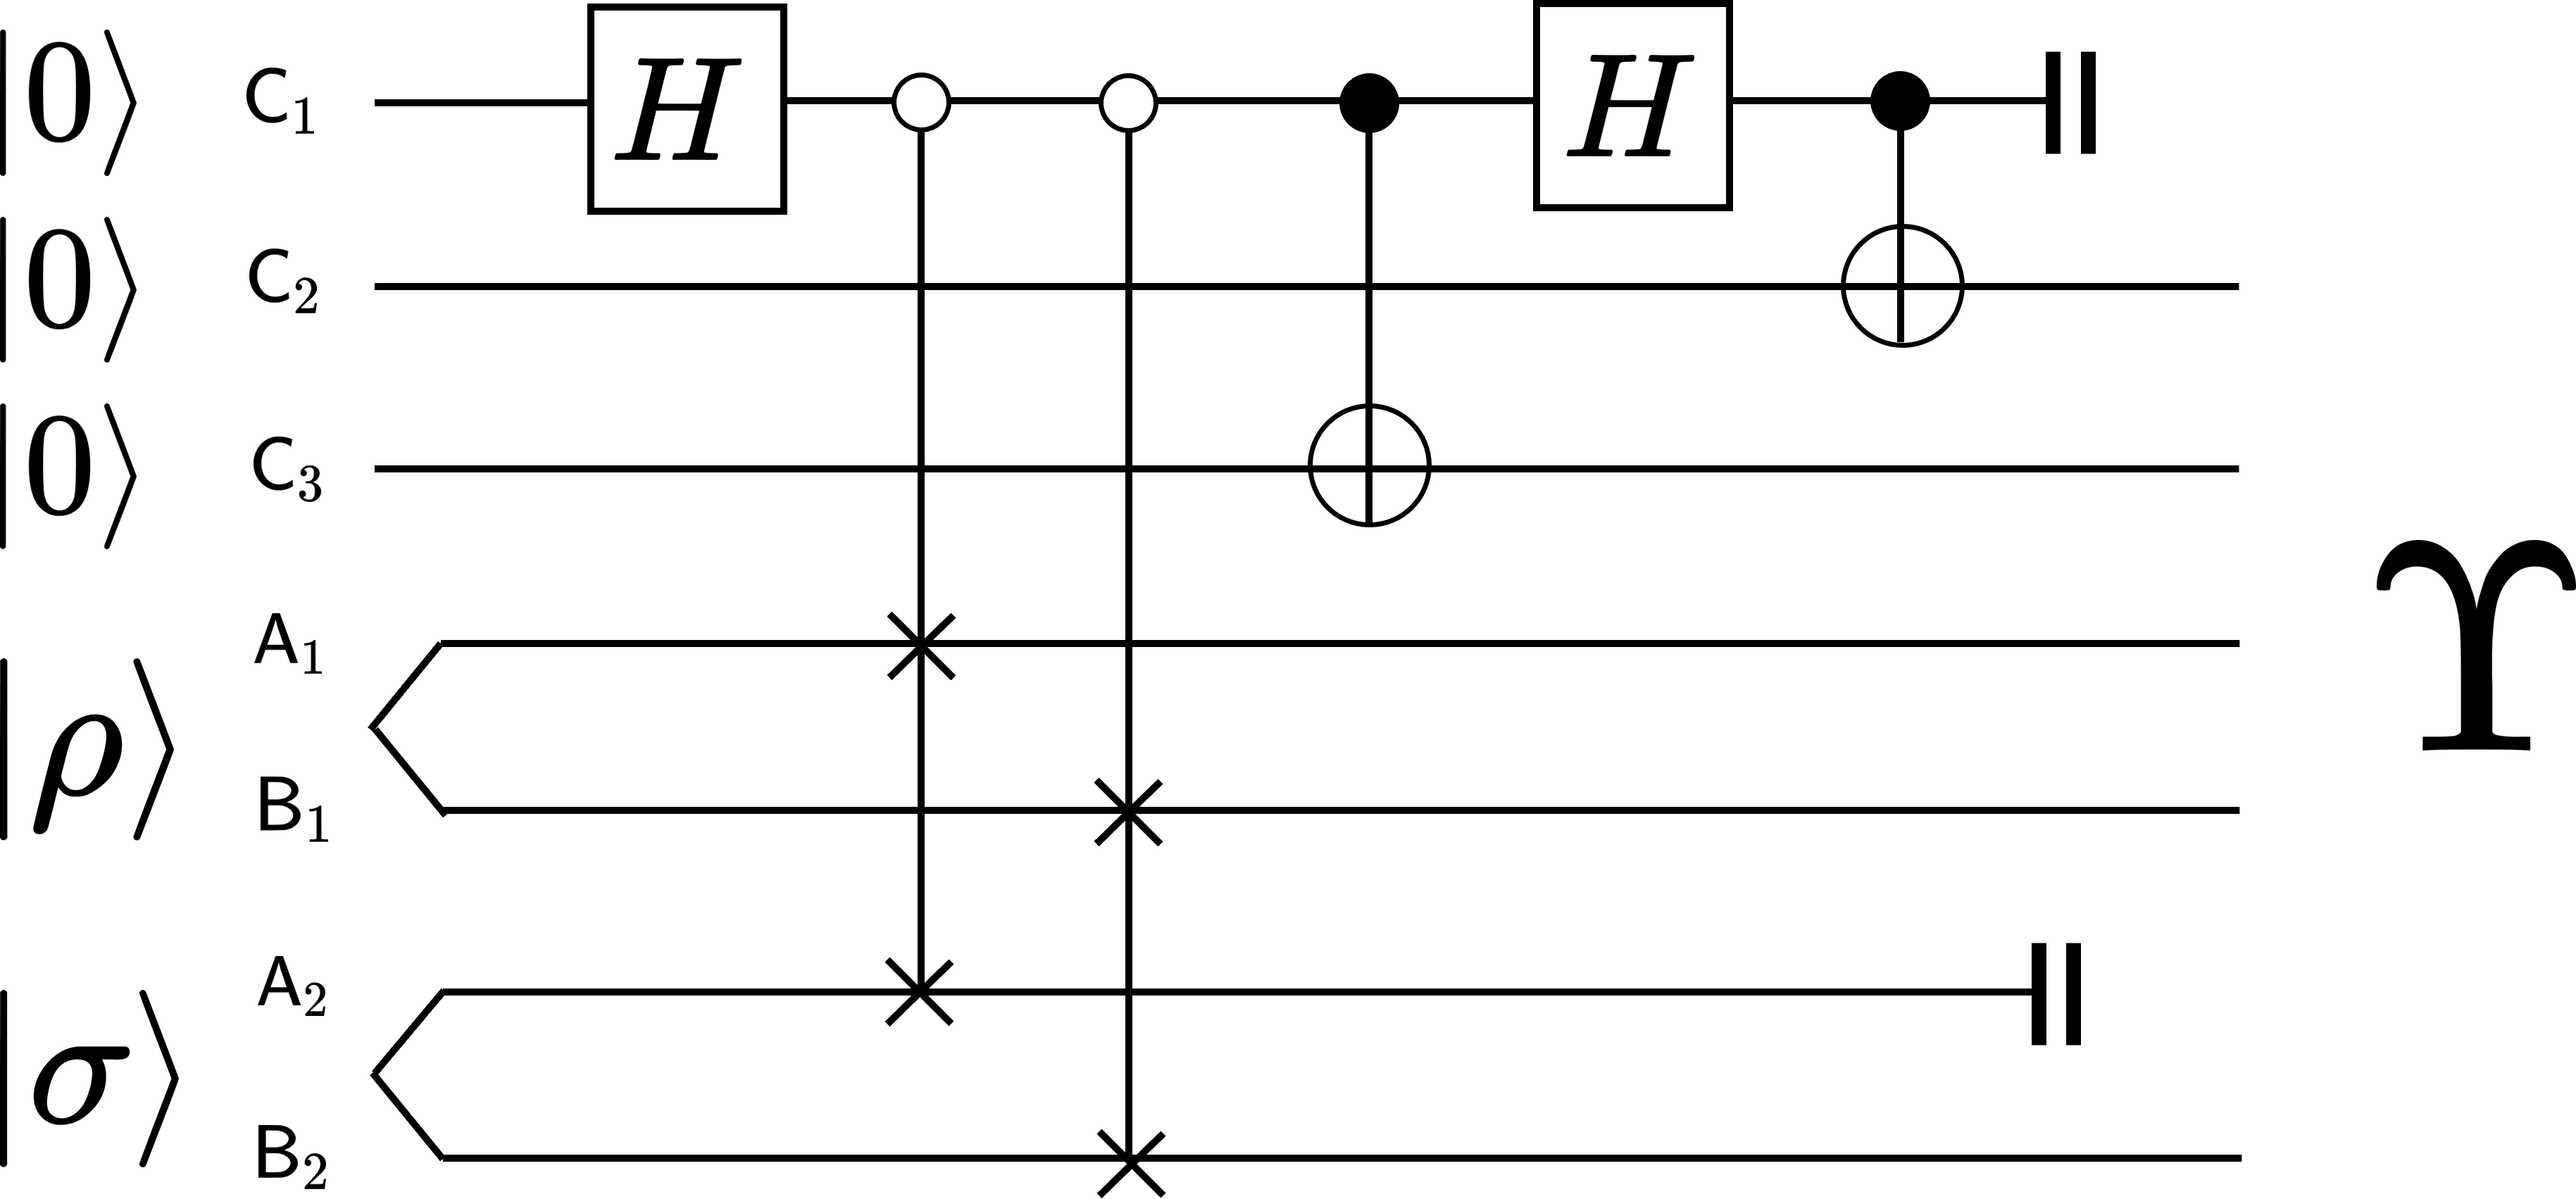
\includegraphics[width=90mm]{fig1.png}
    \caption{A quantum circuit preparing the state $\Upsilon$ in Eq.~\eqref{inteq:64}.
    The systems $\sC_1$, $\sC_2$, and $\sC_3$ are each one-qubit systems. Open circles indicate that the gate is applied when the control qubit is in the state $\ket{0}$, while closed circles indicate control for a qubit in the state $\ket{1}$. The gate $H$ is the one-qubit Hadamard gate. The double vertical lines represent that the qubits of that system are traced out. By convention, the objects with a cross mark and a circle with a cross represent the swap operator and the NOT operator, respectively.}
    \label{fig:upsilon circuit}
\end{figure}














In step 1, we denote by $\Upsilon^{\sC_2\sC_3\sA_1\sB_1\sB_2}$ the output state of the quantum circuit given in \Cref{fig:upsilon circuit}, where each of $\sC_1$, $\sC_2$, and $\sC_3$ is a one-qubit system.
From a direct calculation, we see that $\Upsilon^{\sC_2\sC_3\sA_1\sB_1\sB_2}$ is the form
\begin{align}
\label{inteq:64}
    \Upsilon^{\sC_2\sC_3\sA_1\sB_1\sB_2} 
    = \f{1}{2}\big(\ketbra{0}{0}^{\sC_2} \otimes \xi^{\sC_3\sA_1\sB_1\sB_2} 
    + \ketbra{1}{1}^{\sC_2} \otimes Z^{\sC_3}\xi^{\sC_3\sA_1\sB_1\sB_2} Z^{\sC_3}\big),
\end{align}
where $Z^{\sC_3}$ is the one-qubit Pauli-$Z$ operator acting on $\sC_3$.
The state $\xi^{\sC_3\sA_1\sB_1\sB_2}$ is given by
\begin{align}
    \xi^{\sC_3\sA_1\sB_1\sB_2}
    &= \f{1}{2}\tr_{\sA_2}\big[\big(\ket{0}^{\sC_3}\ket{\sigma}^{\sA_1\sB_1}\ket{\rho}^{\sA_2\sB_2}+\ket{1}^{\sC_3}\ket{\rho}^{\sA_1\sB_1}\ket{\sigma}^{\sA_2\sB_2}\big) \notag \\
    &\hspace{9pc}\big(\bra{0}^{\sC_3}\bra{\sigma}^{\sA_1\sB_1}\bra{\rho}^{\sA_2\sB_2}+\bra{1}^{\sC_3}\bra{\rho}^{\sA_1\sB_1}\bra{\sigma}^{\sA_2\sB_2}\big)\big] \\
    &= \f{1}{2}
\begin{blockarray}{ccc}
& \bra{0}^{\sC_3}&  \bra{1}^{\sC_3} \vspace{1mm}\\
\begin{block}{c(cc)}
  \ket{0}^{\sC_3}\hspace*{1mm} & \ketbra{\sigma}{\sigma}^{\sA_1\sB_1}\otimes\rho^{\sB_2} & \ketbra{\sigma}{\rho}^{\sA_1\sB_1}\otimes (M^{\sB_2})^\dag \\
  \ket{1}^{\sC_3}\hspace*{1mm} & \ketbra{\rho}{\sigma}^{\sA_1\sB_1}\otimes M^{\sB_2} & \ketbra{\rho}{\rho}^{\sA_1\sB_1}\otimes\sigma^{\sB_2} \\
\end{block}
\end{blockarray}\hspace{2.5mm}.
\end{align}
where $M^{\sB_2} = \tr_{\sA_1}\big[\ketbra{\sigma}{\rho}^{\sA_1\sB_2}\big]$.
Since the signs of the off-diagonal entries are flipped by $Z^{\sC_3}$, the state $Z^{\sC_3}\xi^{\sC_3\sA_1\sB_1\sB_2}Z^{\sC_3}$ is given by 
\begin{align}
    Z^{\sC_3}\xi^{\sC_3\sA_1\sB_1\sB_2}Z^{\sC_3}
    = \f{1}{2}
\begin{blockarray}{ccc}
& \bra{0}^{\sC_3}&  \bra{1}^{\sC_3} \vspace{1mm}\\
\begin{block}{c(cc)}
  \ket{0}^{\sC_3}\hspace*{1mm} & \ketbra{\sigma}{\sigma}^{\sA_1\sB_1}\otimes\rho^{\sB_2} & -\ketbra{\sigma}{\rho}^{\sA_1\sB_1}\otimes (M^{\sB_2})^\dag \\
  \ket{1}^{\sC_3}\hspace*{1mm} & -\ketbra{\rho}{\sigma}^{\sA_1\sB_1}\otimes M^{\sB_2} & \ketbra{\rho}{\rho}^{\sA_1\sB_1}\otimes\sigma^{\sB_2} \\
\end{block}
\end{blockarray}\hspace{2mm}.
\end{align}



For step 2, from \Cref{prevthm:DME variant} with $t=2$, we can approximately realize a unitary $e^{iK^{\sC\hat{\sA}\hat{\sB}\sB}}$ within the error $\delta_2$ by using $\mathtt{DMESUB}$ with $m$ copies of $\Upsilon^{\sC_2\sC_3\sA_1\sB_1\sB_2}$, where 
\begin{equation}
\label{eq:m}
m = \Big\lceil\f{16}{\delta_2}\Big\rceil.
\end{equation}
Here, $K^{\sC\hat{\sA}\hat{\sB}\sB}$ is given by
\begin{align}
\label{eq:def of L}
    K^{\sC\hat{\sA}\hat{\sB}\sB} 
    = \xi^{\sC\hat{\sA}\hat{\sB}\sB} - Z^{\sC}\xi^{\sC\hat{\sA}\hat{\sB}\sB}Z^{\sC}
    = 
\begin{blockarray}{ccc}
& \bra{0}^{\sC}&  \bra{1}^{\sC} \vspace{1mm}\\
\begin{block}{c(cc)}
  \ket{0}^{\sC}\hspace*{1.5mm} & 0 & \ketbra{\sigma}{\rho}^{\hat{\sA}\hat{\sB}}\otimes (M^{\sB})^\dag \\
  \ket{1}^{\sC}\hspace*{1.5mm} & \hspace*{0.5mm} \ketbra{\rho}{\sigma}^{\hat{\sA}\hat{\sB}}\otimes M^{\sB} & 0 \\
\end{block}
\end{blockarray}\hspace{2.5mm},
\end{align}
which is an Hermitian matrix with zero diagonal entries.
Although the parameter $t$ can be set to other values, we fix $t = 2$ for simplicity.



Before proceeding to step~3, we examine the structure of the unitary $e^{iK}$. 
For a matrix $A$ with the singular value decomposition $A = \sum_j a_j \ketbra{\eta_j}{\xi_j}$, we define the action of sine and cosine functions on $A$ as
\begin{align}
    &\sin^{(\rm SV)}(A) = \sum_j \sin(a_j)\ketbra{\eta_j}{\xi_j}, \ \ \text{and} \ \ \ \cos^{(\rm SV)}(A) = \sum_j \cos(a_j)\ketbra{\xi_j}{\xi_j}.
\end{align}
Then, the unitary $e^{iK}$ can be rephrased as
\begin{align}
\label{eq:block rep. e^{itK}}
    e^{iK^{\sC\hat{\sA}\hat{\sB}\sB}}
    = \hspace{1mm}
\begin{blockarray}{ccc}
& \bra{0}^{\sC}&  \bra{1}^{\sC} \vspace{1mm}\\
\begin{block}{c(cc)}
  \ket{0}^{\sC}\hspace*{1.5mm} & \cos^{(\rm SV)}(L) & i\sin^{(\rm SV)}(L^\dag) \\
  \ket{1}^{\sC}\hspace*{1.5mm} & i\sin^{(\rm SV)}(L) & \cos^{(\rm SV)}(L^\dag) \\
\end{block}
\end{blockarray}\hspace{2.5mm},
\end{align}
where $L^{\hat{\sA}\hat{\sB}\sB} = \ketbra{\rho}{\sigma}^{\hat{\sA}\hat{\sB}}\otimes M^{\sB}$ and $M^\sB = \tr_{\sA'}\big[\ketbra{\sigma}{\rho}^{\sA'\sB}\big]$.


To see this, let the singular value decomposition of $L^{\hat{\sA}\hat{\sB}\sB}$ be given by $L^{\hat{\sA}\hat{\sB}\sB} = \sum_j s_j \ketbra{l_j}{r_j}^{\hat{\sA}\hat{\sB}\sB}$, and we define $\ket{\psi_j^+}^{\sC\hat{\sA}\hat{\sB}\sB}$ and $\ket{\psi_j^-}^{\sC\hat{\sA}\hat{\sB}\sB}$ by
\begin{align}
    &\ket{\psi_j^+}^{\sC\hat{\sA}\hat{\sB}\sB} = \f{1}{\sqrt{2}}(\ket{0}^\sC \ket{r_j}^{\hat{\sA}\hat{\sB}\sB} + \ket{1}^\sC \ket{l_j}^{\hat{\sA}\hat{\sB}\sB}), \ \ \text{and} \ \ \ \ket{\psi_j^-}^{\hat{\sA}\hat{\sB}\sB} = \f{1}{\sqrt{2}}(\ket{0}^\sC \ket{r_j}^{\hat{\sA}\hat{\sB}\sB} - \ket{1}^\sC \ket{l_j}^{\hat{\sA}\hat{\sB}\sB}).
\end{align}
We can see that these states $\ket{\psi_j^+}^{\sC\hat{\sA}\hat{\sB}\sB}$ and $\ket{\psi_j^-}^{\sC\hat{\sA}\hat{\sB}\sB}$ are eigenstates of $K^{\sC\hat{\sA}\hat{\sB}\sB}$ corresponding eigenvalues $s_j$ and $-s_j$, respectively, because $K^{\sC\hat{\sA}\hat{\sB}\sB}\ket{\psi_j^+}^{\sC\hat{\sA}\hat{\sB}\sB} = s_j \ket{\psi_j^+}^{\sC\hat{\sA}\hat{\sB}\sB}$ and $K^{\sC\hat{\sA}\hat{\sB}\sB}\ket{\psi_j^-}^{\sC\hat{\sA}\hat{\sB}\sB} = -s_j \ket{\psi_j^-}^{\sC\hat{\sA}\hat{\sB}\sB}$~\cite{lloyd2020polardecomposition, lloyd2021hamiltonianQSVT, Lin2022LectureNotes, Odake2024Highoder}.
Thus, $K^{\sC\hat{\sA}\hat{\sB}\sB}$ can be decomposed as $K^{\sC\hat{\sA}\hat{\sB}\sB} = \sum_j \big(s_j\ketbra{\psi_j^+}{\psi_j^+}^{\sC\hat{\sA}\hat{\sB}\sB} - s_j \ketbra{\psi_j^-}{\psi_j^-}^{\sC\hat{\sA}\hat{\sB}\sB} \big)$.
Hence, the unitary $e^{iK}$ can be rewritten as
\begin{align}
    e^{iK}
    &= \sum_j \big(e^{i s_j}\ketbra{\psi_j^+}{\psi_j^+} + e^{-i s_j} \ketbra{\psi_j^-}{\psi_j^-}\big) \\
    &= \sum_j \Big(\f{e^{i s_j}+e^{-i s_j}}{2}\big(\ketbra{0}{0} \otimes \ketbra{r_j}{r_j} 
    + \ketbra{1}{1} \otimes \ketbra{l_j}{l_j}\big) \notag\\
    &\hspace{6pc}+ \f{e^{i s_j}-e^{-i s_j}}{2}\big(\ketbra{0}{1} \otimes \ketbra{r_j}{l_j}
    + \ketbra{1}{0} \otimes \ketbra{l_j}{r_j}\big)\Big) \\
    &= \ketbra{0}{0} \otimes \cos^{(\rm SV)}(L) + \ketbra{1}{1} \otimes \cos^{(\rm SV)}(L^\dag) \notag\\
    &\hspace{6pc}+ \ketbra{0}{1} \otimes i\sin^{(\rm SV)}(L^\dag) + \ketbra{1}{0} \otimes i\sin^{(\rm SV)}(L).
\end{align}





Let $U_2^{\sC\hat{\sA}\hat{\sB}\sB} = -iX^\sC e^{iK^{\sC\hat{\sA}\hat{\sB}\sB}}$, where $X^\sC$ is the one-qubit Pauli-$X$ gate on the system $\sC$. Since $e^{iK^{\sC\hat{\sA}\hat{\sB}\sB}}$ is given in Eq.~\eqref{eq:block rep. e^{itK}}, we see that $U_2^{\sC\hat{\sA}\hat{\sB}\sB}$ is a block-encoding unitary of $\sin^{(\rm SV)}(L^{\hat{\sA}\hat{\sB}\sB}) = \ketbra{\rho}{\sigma}^{\hat{\sA}\hat{\sB}} \otimes \sin^{(\rm SV)}(M^\sB)$:
\begin{align}
    U_2^{\sC\hat{\sA}\hat{\sB}\sB}
    &= \hspace{1mm}
\begin{blockarray}{ccc}
& \bra{0}^\sC &  \vspace{1mm}\\
\begin{block}{c(cc)}
  \ket{0}^\sC \hspace*{1mm} & \ketbra{\rho}{\sigma}^{\hat{\sA}\hat{\sB}}\otimes \sin^{(\rm SV)}\big(M^\sB\big) & \hspace{0mm} * \hspace{3mm}\\
  & * & \hspace{0mm} * \hspace{3mm}\\
\end{block}
\end{blockarray}\hspace{2.5mm}.
\end{align}
The term $\ketbra{\sigma}{\rho}^{\hat{\sA}\hat{\sB}}$ is irrelevant to the singular values.
Although the coefficient $-i$ is clearly not essential since $-iX(\cdot)(-iX)^\dag = X(\cdot)X$, it is introduced here for simplicity.
Noting that the diamond norm is invariant under unitaries, we can obtain a quantum channel $\cG^{\sC\hat{\sA}\hat{\sB}\sB}$ that satisfies
\begin{equation}
\label{eq:matrix exponentiation of M}
    \f{1}{2}\|\cG^{\sC\hat{\sA}\hat{\sB}\sB} - \cU_2^{\sC\hat{\sA}\hat{\sB}\sB}\|_\diamond \leq \delta_2,
\end{equation}
by $\mathtt{DMESUB}(\Upsilon^{\sC_2\sC_3\sA_1\sB_1\sB_2}; \delta_2, t=2)$.


By using $\mathtt{DMESUB}^\dag$ instead of $\mathtt{DMESUB}$, we can approximate $e^{-iK^{\sC\hat{\sA}\hat{\sB}\sB}}$ from $\Upsilon^{\sC_2\sC_3\sA_1\sB_1\sB_2}$, and hence approximate $(U_2^{\sC\hat{\sA}\hat{\sB}\sB})^\dag = ie^{-iK^{\sC\hat{\sA}\hat{\sB}\sB}} X^\sC$. That is, we can obtain a quantum channel $\cG_{\rm inv}^{\sC\hat{\sA}\hat{\sB}\sB}$ such that
\begin{align}
\label{inteq:92}
    \f{1}{2}\big\|\cG_{\rm inv}^{\sC\hat{\sA}\hat{\sB}\sB} - (\cU_2^{\sC\hat{\sA}\hat{\sB}\sB})^\dag\big\|_\diamond \leq \delta_2,    
\end{align}
using $\mathtt{DMESUB}^\dag$ that takes the same number of samples and gates as $\mathtt{DMESUB}$.


Since $M^\sB = \tr_{\sA'}\big[\ketbra{\sigma}{\rho}^{\sA'\sB}\big]$, we obtain $\ketbra{\rho}{\sigma}^{\hat{\sA}\hat{\sB}} \otimes V^\sB$ by lifting up all the singular values of $\ketbra{\rho}{\sigma}^{\hat{\sA}\hat{\sB}}\otimes \sin^{(\rm SV)}\big(M^\sB\big)$ to unity, where $V^\sB$ is the Uhlmann partial isometry (see also \Cref{prop:explicit form of Uhl}).
To achieve that, we use the QSVT with the sign function in step 3.


Using $\mathtt{QSVTSIGN}$ in \Cref{prop:FPAA general} with input $\cG^{\sC\hat{\sA}\hat{\sB}\sB}$ and $\cG_{\rm inv}^{\sC\hat{\sA}\hat{\sB}\sB}$, we can realize a quantum channel $\cJ^{\sB\sH\hat{\sA}\hat{\sB}}$ that satisfies
\begin{equation}
\label{inteq:16}
    \f{1}{2}\big\|\cJ^{\sB\sH\hat{\sA}\hat{\sB}} - \cU_1^{\sB\sH\hat{\sA}\hat{\sB}}\big\|_\diamond \leq u\delta_2,
\end{equation}
where $\sH$ is a two-qubit system and $u$ is the minimum odd integer such that 
\begin{align} 
\label{eq:u} 
    u \geq \Big\lceil \f{8 e}{\beta}\log{\Big(\f{2}{\delta_1}\Big)} \Big\rceil.
\end{align}
The unitary $U_1^{\sH\hat{\sA}\hat{\sB}\sH}$ is given by
\begin{align}
\label{inteq:61}
    U_1^{\sB\sH\hat{\sA}\hat{\sB}} 
    = \hspace{1mm}
\begin{blockarray}{ccc}
& \bra{0^2}^\sH&  \vspace{1mm}\\
\begin{block}{c(cc)}
  \ket{0^2}^\sH \hspace*{1mm} & \ketbra{\rho}{\sigma}^{\hat{\sA}\hat{\sB}}\otimes P_\sgn^{(\rm SV)}\big(\sin^{(\rm SV)}(M^\sB)\big) & \hspace{0mm} * \hspace{3mm}\\
  & * & \hspace{0mm} * \hspace{3mm}\\
\end{block}
\end{blockarray}\hspace{2.5mm},
\end{align}
where $P_\sgn$ satisfies $|P_\sgn(x) - \sgn(x)| \leq \delta_1$ for $x \in [\beta, 1]$.
This follows from replacing $U_2^{\sC\hat{\sA}\hat{\sB}\sB}$ and $(U_2^{\sC\hat{\sA}\hat{\sB}\sB})^\dag$, used a total of $u$ times in the quantum circuit for $\mathtt{QSVTSIGN}$, with a channel $\cG^{\sC\hat{\sA}\hat{\sB}\sB}$ and $\cG_{\rm inv}^{\sC\hat{\sA}\hat{\sB}\sB}$, respectively, which approximate these unitaries as Eqs.~\eqref{eq:matrix exponentiation of M} and~\eqref{inteq:92}.
The overall error is evaluated using the subadditivity of the diamond norm.
Note that
\begin{align}
    P_\sgn^{(\rm SV)}\big(\ketbra{\sigma}{\rho}^{\hat{\sA}\hat{\sB}} \otimes \sin^{(\rm SV)}(M^\sB)\big)
    = \ketbra{\sigma}{\rho}^{\hat{\sA}\hat{\sB}} \otimes P_\sgn^{(\rm SV)}\big(\sin^{(\rm SV)}(M^\sB)\big).
\end{align}




The discussion so far is applicable to both cases, where the performance of our algorithm is measured by either the diamond norm or the fidelity difference.
In the following, we evaluate these two cases separately.
In \Cref{sec:FPAA part}, we provide a proof with the approximation error measured by the diamond norm, while in \Cref{sec:uhlfidquery}, we focus on the fidelity difference, which leads to fewer samples.
These results give the full statement of Theorem~\ref{thm:algorithm Uhlmann}.





%=============================================================================================================================================================================
%=============================================================================================================================================================================





\subsubsection{Evaluation in the diamond norm}
\label{sec:FPAA part}


We evaluate a distance between $U_1^{\sB\sH\hat{\sA}\hat{\sB}}$ and a unitary $U_{\rm ideal}^{\sB\sH}$ which is an exact block-encoding of $\ketbra{\rho}{\sigma}^{\hat{\sA}\hat{\sB}}\otimes\sgn^{(\rm SV)}\big(\sin^{(\rm SV)}(M^\sB)\big)$:
\begin{align}
    U_{\rm ideal}^{\sB\sH\hat{\sA}\hat{\sB}} 
    = \hspace{1mm}
\begin{blockarray}{ccc}
& \bra{0^2}^\sH&  \vspace{1mm}\\
\begin{block}{c(cc)}
  \ket{0^2}^\sH \hspace*{1mm} & \ketbra{\rho}{\sigma}^{\hat{\sA}\hat{\sB}}\otimes \sgn^{(\rm SV)}\big(\sin^{(\rm SV)}(M^\sB)\big) & \hspace{0mm} * \hspace{3mm}\\
  & * & \hspace{0mm} * \hspace{3mm}\\
\end{block}
\end{blockarray}\hspace{2.5mm}.
\end{align}
We note that $\sgn^{(\rm SV)}\big(\sin^{(\rm SV)}(M^\sB)\big)$ corresponds to the Uhlmann partial isometry $V^\sB$ because the singular values of $M^\sB$ correspond to those of $\sqrt{\sigma^\sA}\sqrt{\rho^\sA}$, hence all lie within $[0, 1]$, and in $x \in [0, 1]$, $0 \leq \sin(x) \leq 1$. 

The function $\sin(x)$ increases monotonically in $x \in [0, 1]$ and satisfies $\f{2}{\pi} x \leq \sin(x)$.
Thus, by setting $\beta$ as $\beta = \beta_\diamond = \f{2}{\pi}s_{\rm min}$, where $s_{\min}$ is the minimum non-zero singular value of $\sqrt{\sigma^\sA}\sqrt{\rho^\sA}$, from \Cref{prop:FPAA general}, we have that
\begin{align}
\label{inteq:89}
    \big\|P_\sgn^{(\rm SV)}\big(\sin^{(\rm SV)}(M^\sB)\big) - \sgn^{(\rm SV)}\big(\sin^{(\rm SV)}(M^\sB)\big)\big\|_\infty \leq \delta_1.
\end{align}
From \Cref{lem:FPAA diamond}, when Eq.~\eqref{inteq:89} holds, we obtain that
\begin{align}
\label{inteq:25}
    \f{1}{2}\big\|\cU_1^{\sB\sH\hat{\sA}\hat{\sB}}\circ\cP_{\ket{0}\ket{\sigma}}^{\bC\rarr\sH\hat{\sA}\hat{\sB}} - \cU_{\rm ideal}^{\sB\sH\hat{\sA}\hat{\sB}}\circ\cP_{\ket{0}\ket{\sigma}}^{\bC\rarr\sH\hat{\sA}\hat{\sB}}\big\|_\diamond \leq 3\sqrt{\delta_1},
\end{align}
where $\cP_{\ket{0}\ket{\sigma}}^{\bC\rarr\sH\hat{\sA}\hat{\sB}} = \ketbra{0^2}{0^2}^\sH \otimes \ketbra{\sigma}{\sigma}^{\hat{\sA}\hat{\sB}}$.
Note that, in the purified sample access model, we can easily implement the channel $\cP_{\ket{\sigma}}^{\bC\rarr\hat{\sA}\hat{\sB}}$, since it only involves assigning one of the given copies of $\ket{\sigma}^{\hat{\sA}\hat{\sB}}$.



Finally, we evaluate the total error of the whole algorithm using the triangle inequality. 
We can evaluate the error as
\begin{align}
    \big\|\cJ^{\sB\sH\hat{\sA}\hat{\sB}}\circ\cP_{\ket{0}\ket{\sigma}}^{\bC\rarr\sH\hat{\sA}\hat{\sB}} - \cU_{\rm ideal}^{\sB\sH\hat{\sA}\hat{\sB}}\circ\cP_{\ket{0}\ket{\sigma}}^{\bC\rarr\sH\hat{\sA}\hat{\sB}}\big\|_\diamond  
    &\leq \big\|\cJ^{\sB\sH\hat{\sA}\hat{\sB}}\circ\cP_{\ket{0}\ket{\sigma}}^{\bC\rarr\sH\hat{\sA}\hat{\sB}} - \cU_1^{\sB\sH\hat{\sA}\hat{\sB}}\circ\cP_{\ket{0}\ket{\sigma}}^{\bC\rarr\sH\hat{\sA}\hat{\sB}}\big\|_\diamond     \notag\\
    &\hspace{3pc}+ \big\|\cU_1^{\sB\sH\hat{\sA}\hat{\sB}}\circ\cP_{\ket{0}\ket{\sigma}}^{\bC\rarr\sH\hat{\sA}\hat{\sB}} - \cU_{\rm ideal}^{\sB\sH\hat{\sA}\hat{\sB}}\circ\cP_{\ket{0}\ket{\sigma}}^{\bC\rarr\sH\hat{\sA}\hat{\sB}}\big\|_\diamond \\
    &\leq \big\|\cJ^{\sB\sH\hat{\sA}\hat{\sB}} - \cU_1^{\sB\sH\hat{\sA}\hat{\sB}}\big\|_\diamond \big\|\cP_{\ket{0}\ket{\sigma}}^{\bC\rarr\sH\hat{\sA}\hat{\sB}}\big\|_\diamond    \notag\\
    &\hspace{3pc}+ \big\|\cU_1^{\sB\sH\hat{\sA}\hat{\sB}}\circ\cP_{\ket{0}\ket{\sigma}}^{\bC\rarr\sH\hat{\sA}\hat{\sB}} - \cU_{\rm ideal}^{\sB\sH\hat{\sA}\hat{\sB}}\circ\cP_{\ket{0}\ket{\sigma}}^{\bC\rarr\sH\hat{\sA}\hat{\sB}}\big\|_\diamond.
\end{align}
Thus, as $\big\|\cP_{\ket{0}\ket{\sigma}}^{\bC\rarr\sH\hat{\sA}\hat{\sB}}\big\|_\diamond = 1$, and from Eqs.~\eqref{inteq:16} and~\eqref{inteq:25}, we obtain that, for $\delta_2 \in (0, 1)$ and $\delta_1 \in (0, 1/2)$,
\begin{align}
\label{inteq:103}
    \f{1}{2} \big\|\cJ^{\sB\sH\hat{\sA}\hat{\sB}}\circ\cP_{\ket{0}\ket{\sigma}}^{\bC\rarr\sH\hat{\sA}\hat{\sB}} - \cU_{\rm ideal}^{\sB\sH\hat{\sA}\hat{\sB}}\circ\cP_{\ket{0}\ket{\sigma}}^{\bC\rarr\sH\hat{\sA}\hat{\sB}}\big\|_\diamond
    \leq 3\sqrt{\delta_1} + u\delta_2.
\end{align}
By rescaling these parameters, such as $\delta_1 = (\delta/6)^2$ and $\delta_2 = \delta/(2u)$, the overall error is bounded by $\delta$.


The number of samples $w_\diamond = um$ of $\ket{\rho}^{\hat{\sA}\hat{\sB}}$ and $\ket{\sigma}^{\hat{\sA}\hat{\sB}}$ is given by 
\begin{align}
    w_\diamond 
    &= \cO\Big(\f{1}{\delta_2 \beta_\diamond}\log{\Big(\f{1}{\delta_1}\Big)}\Big) \\
    &= \cO\Big(\f{1}{\delta s_{\rm min}^2}\Big(\log{\Big(\f{1}{\delta}\Big)}\Big)^2\Big),
\end{align}
where $u$ is the minimum odd integers satisfying Eq.~\eqref{eq:u} and $m$ is given by Eq.~\eqref{eq:m}, while we set $\beta = \beta_\diamond = 2 s_{\rm min}/\pi$.


The quantum circuit in \Cref{fig:upsilon circuit} involves a constant number of one- and two-qubit gates, as well as a controlled-swap operation acting on $\log{(d_\sA d_\sB)}$ qubits, which can be implemented using $\cO\big(\log{(d_\sA d_\sB)}\big)$ gates. The entire algorithm consists of $\cO(w_\diamond)$ applications of this circuit.
Hence, the quantum circuit of the algorithm involves $\cO\big(w\log{(d_\sA d_\sB)}\big)$ one- and two-qubit gates.
Note that, although it might be expected that $\cO\big(w_\diamond\log{(d_\sA d_\sB)}\big)$ auxiliary qubits are required, in fact, $\cO\big(\log{(d_\sA d_\sB)}\big)$ qubits suffice at any time, since this algorithm is carried out sequentially.
This qubits includes those for storing the samples of $\ket{\rho}^{\hat{\sA}\hat{\sB}}$ and $\ket{\sigma}^{\hat{\sA}\hat{\sB}}$, and the constant number of additional qubits.












%============================================================================================================================================================





\subsubsection{Evaluation in the fidelity difference}
\label{sec:uhlfidpurifsamp}


When we evaluate the error using the fidelity difference, 
\begin{align}
    \rF(\rho^\sA, \sigma^\sA) - \rF(\cT^\sB(\ketbra{\rho}{\rho}^{\sA\sB}), \ket{\sigma}^{\sA\sB}),
\end{align}
the sample complexity of the Uhlmann transformation could be smaller than $\cO\Big(\big(\log{(1/\delta)}\big)^2/(\delta s_{\rm min}^2)\Big)$ derived in the previous section.
To show this, we modify only the part of step~3 corresponding to the QSVT with the sign function.




First, we consider the difference between 
\begin{align}
    \sqrt{\rF} 
    = \sqrt{\rF}(\rho^\sA, \sigma^\sA)
    = \sqrt{\rF}(V^\sB\ket{\rho}^{\sA\sB}, \ket{\sigma}^{\sA\sB}), \ \ \ \textrm{and} \ \ \ 
    \sqrt{\rF'} 
    = \sqrt{\rF}(U_1^{\sB\sH\hat{\sA}\hat{\sB}}\ket{\rho}^{\sA\sB}\ket{0^2}^\sH\ket{\sigma}^{\hat{\sA}\hat{\sB}}, \ket{\sigma}^{\sA\sB}\ket{0^2}^\sH\ket{\rho}^{\hat{\sA}\hat{\sB}}).
\end{align}
Remember that $V^\sB$ is the Uhlmann partial isometry, $U_1^{\sB\sH\hat{\sA}\hat{\sB}}$ is a block-encoding unitary of $\ketbra{\rho}{\sigma}^{\hat{\sA}\hat{\sB}} \otimes P_\sgn^{(\rm SV)}\big(\sin^{(\rm SV)}(M^\sB)\big)$ (see Eq.~\eqref{inteq:61}), and $M^\sB = \tr_{\sA'}[\ketbra{\sigma}{\rho}^{\sA'\sB}]$.


As the similar calculation in \Cref{sec:uhlfidquery}, we see that
\begin{align}
\label{inteq:120}
    \big|\sqrt{\rF} - \sqrt{\rF'}\big|
    &= \big| |\bra{\sigma}V^\sB\ket{\rho}^{\sA\sB}| - |\bra{\sigma}P_\sgn^{(\rm SV)}\big(\sin^{(\rm SV)}(M)^\sB\big)\ket{\rho}^{\sA\sB}| \big| \\
    &\leq \sum_k \big|1 - P_\sgn\big(\sin(s_k)\big)\big|s_k \notag\\
    \label{inteq:40}
    &= \sum_{k\in I_\beta} \big|1 - P_\sgn\big(\sin(s_k)\big)\big|s_k  + \sum_{k\in \bar{I}_\beta} \big|1 - P_\sgn\big(\sin(s_k)\big)\big|s_k \\
    &\leq \delta_1 + 2 \sum_{k\in \bar{I}_\beta} s_k \\
    &\leq \delta_1 +  \pi\beta r,
\end{align}
where $I_\beta = \{k \in \bN; \beta \leq \sin(s_k)\}$, $\bar{I}_\beta = \{k \in \bN; \beta > \sin(s_k)\}$, and $r$ is the rank of $\sqrt{\sigma^\sA}\sqrt{\rho^\sA}$.
In the last inequality, we use $s_k \leq \f{\pi}{2}\sin(s_k) < \f{\pi}{2}\beta$ for $k \in \bar{I}_\beta$ and $\#\bar{I}_\beta = \sum_{k \in \bar{I}_\beta} 1 \leq r$.



Thus, setting $\beta$ as $1/\beta = \pi r/\delta_1$ ensures $\big|\sqrt{\rF} - \sqrt{\rF'}\big| \leq 2\delta_1$. 
On the other hand, if we choose $1/\beta = \pi/(2s_{\rm min})$, $\bar{I}_\beta$ is empty, which leads to $\big|\sqrt{\rF} - \sqrt{\rF'}\big|\leq \delta_1$.
Hence, $\beta$ is chosen as $\beta = \beta_\tF$, where $1/\beta_\tF = \pi\min\{1/(2s_{\rm min}), r/\delta_1\}$, 
to ensure that 
\begin{align}
\label{inteq:51}
    \big|\sqrt{\rF} - \sqrt{\rF'}| \leq 2\delta_1.
\end{align}
Using that $|x-y|\leq 2|\sqrt{x}-\sqrt{y}|$ for $0\leq x, y \leq 1$, we obtain $\big|\rF - \rF'| \leq 4\delta_1$.

Next, we define $\rF''$ by 
\begin{align}
    \rF'' = \rF\big(\cJ^{\sB\sH\hat{\sA}\hat{\sB}}\circ\cP_{\ket{0}\ket{\sigma}}^{\bC\rarr\sH\hat{\sA}\hat{\sB}}(\ketbra{\rho}{\rho}^{\sA\sB}), \ket{\sigma}^{\sA\sB}\ket{0^2}^\sH\ket{\rho}^{\hat{\sA}\hat{\sB}}\big).
\end{align} 
Then, the difference between $\rF''$ and $\rF$ can be calculated as
\begin{align}
    \big|\rF'' - \rF\big| 
    &\leq \big|\rF'' - \rF'\big| + \big|\rF' - \rF\big| \\
    &\leq\big|\rF'' - \rF'\big| + 4\delta_1 \\
    &\leq \f{1}{2}\big\|\cJ^{\sB\sH\hat{\sA}\hat{\sB}} - \cU_1^{\sB\sH\hat{\sA}\hat{\sB}} \big\|_\diamond + 4\delta_1 \\
    \label{inteq:106}
    &\leq u\delta_2 + 4\delta_1,
\end{align}
where $u$ is given by the minimum odd integer satisfying $u \geq \big\lceil\f{8e}{\beta_\tF}\log{(2/\delta_1)}\big\rceil$.
In the third inequality, we used the relation between the diamond norm and the fidelity Eq.~\eqref{eq:fidelity and diamond} and $\|\cP_{\ket{0}\ket{\sigma}}^{\bC\rarr\sH\hat{\sA}\hat{\sB}}\|_\diamond = 1$.
We also used Eq.~\eqref{inteq:16} in the last inequality.



By rescaling these parameters, such as $\delta_1 = \delta/8$ and $\delta_2 = \delta/(2u)$, and defining $\cT^\sB$ by $\cT^\sB = \tr_{\sH\hat{\sA}\hat{\sB}}\circ\cJ^{\sB\sH\hat{\sA}\hat{\sB}}\circ\cP_{\ket{0}\ket{\sigma}}^{\bC\rarr\sH\hat{\sA}\hat{\sB}}$, we obtain that
\begin{align}
    \rF\big(\cT^\sB(\ketbra{\rho}{\rho}^{\sA\sB}), \ket{\sigma}^{\sA\sB}\big)
    \geq \rF(\rho^\sA, \sigma^\sA) - \delta,
\end{align}
which follows from the fact that $\rF(\rho^\sA, \sigma^\sA) \geq \rF\big(\cT^\sB(\ketbra{\rho}{\rho}^{\sA\sB}), \ket{\sigma}^{\sA\sB}\big)$.
The number of samples $w_\tF = um$ of the states $\ket{\rho}^{\hat{\sA}\hat{\sB}}$ and $\ket{\sigma}^{\hat{\sA}\hat{\sB}}$ is given by
\begin{align}
    w_\tF &= \cO\Big(\f{1}{\delta_2\beta_\tF}\log{\Big(\f{1}{\delta_1}\Big)}\Big) \\
    &= \cO\Big(\f{1}{\delta}\min\Big\{\f{1}{s_{\rm min}^2}, \f{r^2}{\delta^2}\Big\}\Big(\log{\Big(\f{1}{\delta}\Big)}\Big)^2\Big).
\end{align}
The circuit of the algorithm consists of
$\cO\big(w_\tF \log{(d_\sA d_\sB)}\big)$ one- and two-qubit gates, and $\cO(\log{(d_\sA d_\sB)})$ qubits suffice at any one time.
We completed the proof of Theorem~\ref{thm:algorithm Uhlmann}.



%====================================================================================================================================

\section{Uhlmann transformation algorithm in the mixed sample access model}
\label{sec:mixed sample}




We provide a quantum sample algorithm for the Uhlmann transformation in the mixed sample access model.
The key idea for construction is to use a property of the maximally entangled state $\ket{\Phi}^{\sA\sB} = \f{1}{\sqrt{d_\sA}}\sum_{i=1}^{d_\sA}\ket{i}^\sA\ket{i}^{\sB}$: for any state $\omega^\sA$,
\begin{equation}
(\sqrt{\omega^\sA} \otimes \bI^{\sB})\ket{\Phi}^{\sA\sB}
= \f{1}{\sqrt{d_\sA}}\ket{\omega_{\rm c}}^{\sA\sB},
\end{equation}
where $\ket{\omega_{\rm c}}^{\sA\sB}$ is the canonical purified state of $\omega^\sA$. 
Note that $\tr_\sB[\ketbra{\omega_{\rm c}}{\omega_{\rm c}}^{\sA\sB}] = \omega^\sA$.
It is natural to assume that $d_\sA = d_\sB$ in this model.
Our approach is to first prepare canonical purified states $\ket{\rho_{\rm c}}^{\sA\sB}$ and $\ket{\sigma_{\rm c}}^{\sA\sB}$ from multiple copies of given states $\rho^{\hat{\sA}}$ and $\sigma^{\hat{\sA}}$, and then to perform the Uhlmann transformation algorithm for the purified sample access model described in the previous section.  
This is to find the Uhlmann transformation from $\ket{\rho_{\rm c}}^{\sA\sB}$ to $\ket{\sigma_{\rm c}}^{\sA\sB}$.


The statement is as follows, where the system $\sH$ is a two-qubit system. 
Remember that $s_{\rm min}$ and $r$ are the minimum non-zero singular value and the rank of $\sqrt{\sigma^\sA}\sqrt{\rho^\sA}$, respectively. Also, $\rho_{\rm min}$ and $\sigma_{\rm min}$ are the minimum non-zero eigenvalues of $\rho^\sA$ and $\sigma^\sA$, respectively.





\begin{theorem}[Uhlmann transformation algorithm in the mixed sample access model]
\label{thm:Uhlmann mixed state sample}
Let $\delta \in (0, 1)$ and $\chi \in \{\diamond, \tF\}$. 
Then, the quantum sample algorithm $\mathtt{UhlmannMixedSample}$ given by \Cref{alg:Uhl mixed sample} satisfies the following.

A quantum channel $\cJ_\diamond^{\sB\sH\hat{\sA}\hat{\sB}}$ given by $\cJ_\diamond^{\sB\sH\hat{\sA}\hat{\sB}}\circ\cP_{\til{\sigma}_{\rm c}}^{\bC\rarr\hat{\sA}\hat{\sB}}  
    =\mathtt{UhlmannMixedSample}(\rho^{\hat{\sA}}, \sigma^{\hat{\sA}}; \delta, \diamond)$,
with some state $\til{\sigma}_{\rm c}^{\hat{\sA}\hat{\sB}}$, satisfies that
\begin{equation}
    \f{1}{2}\big\|\cJ_\diamond^{\sB\sH\hat{\sA}\hat{\sB}}\circ\cP_{\ket{0}}^{\bC\rarr\sH}\circ\cP_{\til{\sigma}_{\rm c}}^{\bC\rarr\hat{\sA}\hat{\sB}} - \cU_{\rm ideal}^{\sB\sH\hat{\sA}\hat{\sB}}\circ\cP_{\ket{0}\ket{\sigma_{\rm c}}}^{\bC\rarr\sH\hat{\sA}\hat{\sB}}\big\|_\diamond \leq \delta,
\end{equation}
where $\til{U}_{\rm ideal}^{\sB\sH\hat{\sA}\hat{\sB}}$ is an exact block-encoding unitary of $\ketbra{\rho_{\rm c}}{\sigma_{\rm c}}^{\hat{\sA}\hat{\sB}} \otimes V^\sB$ and $V^\sB$ is the Uhlmann partial isometry.
The algorithm uses
\begin{align}
    \zeta_\diamond = \til{\cO}\Big(\f{d_\sA}{\delta^2 s_{\rm min}^3} \min\Big\{\f{1}{\rho_{\rm min}^2} + \f{1}{\sigma_{\rm min}^2}, \f{d_\sA^2}{\delta^4 s_{\rm min}^4}\Big\}\Big),
\end{align}
samples of $\rho^{\hat{\sA}}$ and $\sigma^{\hat{\sA}}$.

A quantum channel $\cJ_\tF^{\sB\sH\hat{\sA}\hat{\sB}}$ given by $\cJ_\tF^{\sB\sH\hat{\sA}\hat{\sB}}\circ\cP_{\til{\sigma}_{\rm c}}^{\bC\rarr\hat{\sA}\hat{\sB}} 
    = \mathtt{UhlmannMixedSample}(\rho^{\hat{\sA}}, \sigma^{\hat{\sA}}; \delta, \tF)$,
with some state $\til{\sigma}_{\rm c}^{\hat{\sA}\hat{\sB}}$, satisfies that
\begin{align}
    \rF\big(\cT^\sB(\ketbra{\rho_{\rm c}}{\rho_{\rm c}}^{\sA\sB}), \ket{\sigma_{\rm c}}^{\sA\sB}\big) \geq \rF(\rho^\sA, \sigma^\sA) - \delta,
\end{align}
where $\cT^{\sB}= \tr_{\sH\hat{\sA}\hat{\sB}}\circ\cJ_\tF^{\sB\sH\hat{\sA}\hat{\sB}}\circ\cP_{\ket{0}}^{\bC\rarr\sH}\circ\cP_{\til{\sigma}_{\rm c}}^{\bC\rarr\hat{\sA}\hat{\sB}}$.
The algorithm uses 
\begin{align}
    \zeta_{\tF} = \til{\cO}\Big(\f{d_\sA}{\delta^2\beta_\tF^3}\min\Big\{\f{1}{\rho_{\rm min}^2} + \f{1}{\sigma_{\rm min}^2}, \f{d_\sA^2}{\beta_\tF^4\delta^4}\Big\}\Big),
\end{align}
samples of $\rho^{\hat{\sA}}$ and $\sigma^{\hat{\sA}}$, where $\beta_\tF = \f{2}{\pi}\max\{s_{\rm min}, \delta/(8r)\}$.

In both cases, the quantum circuit for implementing the algorithm consists of $\cO\big(\zeta_\chi \log{d_\sA}\big)$ one- and two-qubit gates, and $\cO\big(\log{d_\sA}\big)$ qubits suffice at any one time. 
\end{theorem}




\begin{algorithm}[h]
\caption{Uhlmann transformation algorithm in the mixed sample access model \\ \parbox{\linewidth}{\centering $\mathtt{UhlmannMixedSample}(\rho^{\hat{\sA}}, \sigma^{\hat{\sA}}; \delta, \chi)$ (In Theorem~\ref{thm:Uhlmann mixed state sample})}}
\label{alg:Uhl mixed sample}
\SetKwInput{KwInput}{Input}
\SetKwInput{KwOutput}{Output}
\SetKwInput{KwParameters}{Parameters}
\SetKwComment{Comment}{$\triangleright$\ }{}
\SetCommentSty{textnormal}
\SetKwProg{Fn}{Subroutine}{}{end}
\SetKwFunction{UPS}{UhlmannPurifiedSample}

\SetAlgoNoEnd
\SetAlgoNoLine
\KwInput{Two quantum states $\rho^{\hat{\sA}}$ and $\sigma^{\hat{\sA}}$.}
\KwParameters{$\delta \in (0, 1)$ and $\chi \in \{\diamond, \tF\}$.}
\KwOutput{Quantum channel $\cJ^{\sB\sH\hat{\sA}\hat{\sB}}\circ\cP_{\til{\sigma}_{\rm c}}^{\bC\rarr\hat{\sA}\hat{\sB}}$.}
\SetAlgoLined

\If{$\chi = \diamond$}{
  Set $\delta_3 \gets (\delta/12)^2$ and $\beta \gets 2s_{\rm min}/\pi$. \\
}
\ElseIf{$\chi = \tF$}{
  Set $\delta_3 \gets \delta/16$ and $\beta \gets \f{1}{\pi}\max\{2s_{\rm min}, \delta_3/r\}$. \\
}
Set $u$ to be the minimum odd integer satisfying $u \geq \big\lceil\f{8e}{\beta}\log{(2/\delta_3)}\big\rceil$. \\
Set $\delta_1 \gets \delta/\big(2(4u+1)\big)$. \\
Set $\til{\rho}_{\rm c}^{\hat{\sA}\hat{\sB}} \gets \mathtt{CanonicalPurification}(\rho^{\hat{\sA}}; \delta_1)$ and $\til{\sigma}_{\rm c}^{\hat{\sA}\hat{\sB}} \gets \mathtt{CanonicalPurification}(\sigma^{\hat{\sA}}; \delta_1)$ (Algorithm~\ref{alg:canonical purification}). \\
Set $\cJ^{\sB\sH\hat{\sA}\hat{\sB}} \gets \mathtt{UhlmannPurifiedSample}(\til{\rho}_{\rm c}^{\hat{\sA}\hat{\sB}}, \til{\sigma}_{\rm c}^{\hat{\sA}\hat{\sB}}; \delta/2, \chi)$ (Algorithm~\ref{alg:Uhl purif sample}). \\
Set $\cP_{\til{\sigma}_{\rm c}}^{\bC\rarr\hat{\sA}\hat{\sB}} \gets \til{\sigma}_{\rm c}^{\hat{\sA}\hat{\sB}}$. \\
Return $\cJ^{\sB\sH\hat{\sA}\hat{\sB}}\circ\cP_{\til{\sigma}_{\rm c}}^{\bC\rarr\hat{\sA}\hat{\sB}}$. 
\end{algorithm}







In \Cref{alg:Uhl mixed sample}, $\mathtt{CanonicalPurification}$ is a quantum sample algorithm that prepares the states $\til{\rho}_{\rm c}^{\hat{\sA}\hat{\sB}}$ and $\til{\sigma}_{\rm c}^{\hat{\sA}\hat{\sB}}$, which approximate the canonical purified state $\ket{\rho_{\rm c}}^{\hat{\sA}\hat{\sB}}$ and $\ket{\sigma_{\rm c}}^{\hat{\sA}\hat{\sB}}$, respectively. We will introduce and explain this algorithm in detail in the next section, \Cref{sec:appendix B}. 

Note that, although $\mathtt{UhlmannPurifiedSample}$ is originally designed for pure state inputs, in this case, we allow general mixed states as inputs (see \Cref{alg:Uhl mixed sample}).
This requires a careful error analysis, which we will discuss in the proof of Theorem~\ref{thm:Uhlmann mixed state sample} provided in \Cref{sec:proof eval sample mixed}.






%===================================================================================================================================================================================






\subsection{Canonical purification algorithm}
\label{sec:appendix B}

We provide a quantum sample algorithm for the canonical purification $\mathtt{CanonicalPurification}$, which outputs an approximation of the canonical purified state $\ket{\omega_{\rm c}}^{\sA\sB}$ from multiple copies of $\omega^\sA$. 
The details of $\mathtt{CanonicalPurification}$ are provided in \Cref{alg:canonical purification}, where $\sF$ and $\sG$ are five- and six-qubit systems, respectively.
A quantum sample algorithm $\mathtt{BlockEncSqrtState}$ is described in \Cref{prop:block enc sqrt state} below.
Regarding the performance of $\mathtt{CanonicalPurification}$, the following proposition holds.


\begin{theorem}[Quantum algorithm for the canonical purification]
\label{prop:canonical purification}
Let $\delta \in (0, 1)$, and let $\omega^\sA$ be a state whose minimum non-zero eigenvalue is $\omega_{\rm min}$. Then, a quantum sample algorithm $\mathtt{CannonicalPurification}(\omega^\sA; \delta)$ given by \Cref{alg:canonical purification} outputs a state $\til{\omega}_{\rm c}^{\sA\sB}$ such that
\begin{align}
    \f{1}{2}\|\til{\omega}_{\rm c}^{\sA\sB} - \ketbra{\omega_{\rm c}}{\omega_{\rm c}}^{\sA\sB}\|_1 \leq \delta,
\end{align}
using $f = \til{\cO}\Big(\f{d_\sA}{\delta}\min\Big\{\f{1}{\omega_{\rm min}^2}, \f{d_\sA^2}{\delta^4}\Big\}\Big)$ samples of $\omega^\sA$.
The quantum circuit for the algorithm is constructed by $\cO(f\log d_\sA)$ one- and two-qubit gates, and at any one time, $\cO(\log{d_\sA})$ qubits suffice.
\end{theorem}



\begin{algorithm}[h]
\caption{Canonical purification algorithm \\ \parbox{\linewidth}{\centering $\mathtt{CanonicalPurification}(\omega^\sA; \delta)$ (In Theorem~\ref{prop:canonical purification})}}
\label{alg:canonical purification}
\SetKwInput{KwInput}{Input}
\SetKwInput{KwOutput}{Output}
\SetKwInput{KwParameters}{Parameters}
\SetKwComment{Comment}{$\triangleright$\ }{}
\SetCommentSty{textnormal}

\SetAlgoNoEnd
\SetAlgoNoLine
\KwInput{Quantum state $\omega^\sA$.}
\KwParameters{$\delta \in (0, 1)$.}
\KwOutput{Quantum state $\til{\omega}_{\rm c}^{\sA\sB}$.}
\SetAlgoLined


Set $\delta_1 \gets (\delta/6)^2$ and $\beta_\diamond \gets 1/(2\sqrt{2d_\sA})$. \\
Set $u$ to be the minimum odd integer satisfying $u \geq \big\lceil\f{8e}{\beta_\diamond}\log{(2/\delta_1)}\big\rceil$. \\


Set $\cF^{\sA\sF} \gets \mathtt{BlockEncSqrtState}(\omega^\sA; \delta_1/(2u))$ and $\cF_{\rm inv}^{\sA\sF} \gets \mathtt{BlockEncSqrtState}^\dag(\omega^\sA; \delta_1/(2u))$ (Proposition~\ref{prop:block enc sqrt state}). \\
Set $\cG^{\sA\sB\sF} \gets \cF^{\sA\sF}\circ\cU_{\Phi}^{\sA\sB}$ and $\cG_{\rm inv}^{\sA\sB\sF} \gets (\cU_{\Phi}^{\sA\sB})^\dag\circ\cF_{\rm inv}^{\sA\sF}$, where $U_{\Phi}^{\sA\sB}$ is a unitary preparing the maximally entangled state: $U_{\Phi}^{\sA\sB}\ket{0}^{\sA\sB} = \ket{\Phi}^{\sA\sB}$. \\
Set $\cL^{\sA\sB\sG} \gets \mathtt{QSVTSIGN}(\cG^{\sA\sB\sF}, \cG_{\rm inv}^{\sA\sB\sF}; \delta_1, \beta_\diamond)$ (Proposition~\ref{prop:FPAA general}). \\
Set $\til{\omega}_{\rm c}^{\sA\sB} \gets \tr_\sG\circ\cL^{\sA\sB\sG}\circ\cP_{\ket{0}}^{\bC\rarr\sG}(\ketbra{0}{0}^{\sA\sB})$. \\
Return $\til{\omega}_{\rm c}^{\sA\sB}$.
\end{algorithm}



Our approach begins by approximately constructing a unitary, which is a block-encoding of $\sqrt{\omega^\sA}$, using $\mathtt{BlockEncSqrtState}$.
We then apply the unitary to the state $\ket{0}^{\sM}\ket{\Phi}^{\sA\sB}$ and amplify the coefficient to unity by the QSVT with the sign function.



\begin{proposition}
\label{prop:block enc sqrt state}
Let $\delta \in (0, 1)$, and let $\omega$ be a state in a $d$-dimensional Hilbert space, whose minimum non-zero eigenvalue is $\omega_{\rm min}$. 
Then, there is a quantum sample algorithm $\mathtt{BlockEncSqrtState}(\omega; \delta)$ that outputs a channel $\cF$ such that $\f{1}{2}\|\cF - \cU\|_\diamond \leq \delta$, using $h = \til{\cO}\big(\f{1}{\delta}\min\big\{1/\omega_{\rm min}^2, 1/\delta^4\big\}\big)$ samples of $\omega$,
where $U$ is a $(1, 5, 0)$-block-encoding unitary of $\sqrt{\omega}/\big(2\sqrt{2}\big)$.
The quantum circuit for the algorithm consists of $\cO(h\log{d})$ one- and two-qubit gates, and $\cO(\log{d})$ qubits suffice at any one time.

Moreover, there is a quantum sample algorithm $\mathtt{BlockEncSqrtState}^\dag(\omega; \delta)$ that outputs a channel $\cF_{\rm inv}$ such that $\f{1}{2}\|\cF_{\rm inv} - \cU^\dag\|_\diamond \leq \delta$, using the same number of samples, gates, and qubits.
\end{proposition}




We first prove \Cref{prop:block enc sqrt state}.    
At a high level, this is achieved by the following two steps:
\begin{align}
\label{eq:flow of trans purif}
\omega^\sA \overset{1. \, \text{Theorem~\ref{thm:BEquantum state form sample}}}{\longrightarrow}
\begin{pmatrix}
    \omega^\sA & \hspace*{1.5mm} * \hspace*{3mm} \\
    * & \hspace{1.5mm} * \hspace*{3mm}
\end{pmatrix}
\overset{2. \, \text{Proposition~\ref{prop:QSVT sqrt}}}{\longrightarrow}
\begin{pmatrix}
    \sqrt{\omega^\sA} & \hspace*{1.5mm} * \hspace*{3mm} \\
    * & \hspace{1.5mm} * \hspace*{3mm}
\end{pmatrix}.
\end{align}




In step~1, we use quantum algorithms that block-encode the density matrix of a quantum state \cite{gilyen2022improvedfidelity, wang2024fastQAtracedist, wang2023SampletoQuary, wang2024TimeEfficientEntEstSamp}, which are obtained by combining the density matrix exponentiation and the QSVT. 

\begin{theorem}[Block-encoding of a quantum state from samples~{\cite[Lemma 2.21]{wang2023SampletoQuary}}]
\label{thm:BEquantum state form sample}
Let $\delta \in (0, 1)$, and let $\omega$ be a state in a $d$-dimensional Hilbert
space. 
Then, there are quantum sample algorithms that output channels $\cE$ and $\cE_{\rm inv}$, respectively, which satisfy $\f{1}{2}\|\cE - \cU\|_\diamond \leq \delta$ and $\f{1}{2}\|\cE_{\rm inv} - \cU^\dag\|_\diamond \leq \delta$, where $U$ is a $(1, 4, 0)$-block-encoding unitary of $\omega/2$.
Both algorithms use $y$ samples of $\omega$, where $y = \cO\big(\f{1}{\delta}\big(\log{\big(\f{1}{\delta}\big)}\big)^2\big)$.
The quantum circuits for these algorithms consist of $\cO(y\log{d})$ one- and two-qubit gates, and $\cO(\log{d})$ qubits suffice at any one time.
\end{theorem}


In step~2, we use the QSVT to approximate the square root function. 
Specifically, we take the target function for a polynomial approximation to be $\sqrt{x}/2$. This is a special case of the QSVT for positive power functions; see, e.g., Refs.~\cite{Gilyn2019thesis, gilyen2022improvedfidelity, wang2024NewQuantEnt} for details.



\begin{proposition}[QSVT with the square root function~{\cite[Lemma 17 and Corollary 18]{gilyen2022improvedfidelity}},~{\cite[Lemma II.6 and Lemma II.13]{wang2024NewQuantEnt}}]
\label{prop:QSVT sqrt}
Let $\delta \in (0, 1/2)$, and let $U$ be a $(1, a, 0)$-block-encoding unitary of a positive semidefinite matrix $M$ whose minimum non-zero eigenvalue is $m_{\rm min}$. Then, there are quantum algorithms that output unitaries $\til{U}$ and $\til{U}^\dag$, respectively, where $\til{U}$ is a $(1, a+1, 0)$-block-encoding of an even/odd polynomial $R_{\rm sqrt}(M)$.
The polynomial $R_{\rm sqrt}$ satisfies $\big\|R_{\rm sqrt}(M) - \sqrt{M}/2\big\|_\infty \leq \delta$, and $|R_{\rm sqrt}(x)| \leq 1$ for $x \in [-1, 1]$. 
Both algorithms use $U$ and $U^\dag$ a total of $l = \cO\big(\min\{1/m_{\rm min}, 1/\delta^2\}\log{(1/\delta)}\big)$ times.
\end{proposition}

This proposition follows from the existence of polynomials $P_{\rm sqrt}$ and $Q_{\rm sqrt}$, each of which is either even or odd, with degrees $\cO\big(\f{1}{\alpha}\log{(1/\delta)}\big)$ and $\cO\big(\f{1}{\delta^2}\log{(1/\delta)}\big)$, respectively, where $\alpha \in (0, 1/2)$.
These polynomials satisfy that 
\begin{align}
    &\big|P_{\rm sqrt}(x)\big|, \big|Q_{\rm sqrt}(x)\big| \leq 1 
    \ \ \textrm{for} \ \ x \in [-1, 1], \\
    &\Big|P_{\rm sqrt}(x) - \sqrt{x}/2\Big| \leq \delta
    \ \ \textrm{for} \ \ x \in \big[\alpha/2, 1\big], \\
    &\Big|Q_{\rm sqrt}(x) - \sqrt{x}/2\Big| \leq \delta
    \ \ \textrm{for} \ \ x \in [-1, 1].
\end{align}
For our purpose, it suffices to set $\alpha$ so that $\alpha/2 = m_{\rm min}$.



\begin{proof}[Proof of \Cref{prop:block enc sqrt state}]


Let $\delta_1 \in (0, 1)$, and $\sE$ be a four-qubit system.
From Theorem~\ref{thm:BEquantum state form sample}, we can obtain quantum channels $\cE^{\sA\sE}$ and $\cE_{\rm inv}^{\sA\sE}$, which satisfy that
\begin{align}
    \f{1}{2}\big\|\cE^{\sA\sE} - \cU_1^{\sA\sE}\big\|_\diamond \leq \delta_1, \ \ \text{and} \ \ \ 
    \f{1}{2}\big\|\cE_{\rm inv}^{\sA\sE} - (\cU_1^{\sA\sE})^\dag\big\|_\diamond \leq \delta_1,
\end{align}
where $U_1^{\sA\sE}$ is a block- encoding unitary of $\omega/2$, using $y = \cO\Big(\big(\log{(1/\delta_1)}\big)^2/\delta_1\Big)$ samples of $\omega^\sA$.


Let $\delta_2 \in (0, 1/2)$, $\omega_{\rm min}$ be the minimum non-zero eigenvalue of $\omega^\sA$, and $\sF$ be a five-qubit system. 
We evaluate the accumulated error that arises from using quantum channels $\cE^{\sA\sE}$ and $\cE_{\rm inv}^{\sA\sE}$ instead of a unitary $U_1^{\sA\sE}$ and $(U_1^{\sA\sE})^\dag$ in the QSVT with the square root function.
From \Cref{prop:QSVT sqrt}, by using $\cE^{\sA\sE}$ and $\cE_{\rm inv}^{\sA\sE}$ for a total of $l = \cO\big(\min\{1/\omega_{\rm min}, 1/\delta_2^2\}\log{(1/\delta_2)}\big)$ times, we can obtain quantum channels $\cF^{\sA\sF}$ and $\cF_{\rm inv}^{\sA\sF}$ such that 
\begin{align}
\label{inteq:93}
    \f{1}{2}\big\|\cF^{\sA\sF} - \cU_2^{\sA\sF}\big\|_\diamond \leq l\delta_1, \ \  \text{and} \ \ \
    \f{1}{2}\big\|\cF_{\rm inv}^{\sA\sF} - (\cU_2^{\sA\sF})^\dag\big\|_\diamond \leq l\delta_1,
\end{align}
where we used the subadditivity of the diamond norm to bound the overall error.
The unitary $U_2^{\sA\sF}$ is a block-encoding unitary of a polynomial $R_{\rm sqrt}(\omega^\sA/2)$, which satisfies that 
\begin{align}
    \big\|R_{\rm sqrt}(\omega^\sA/2) - \sqrt{\omega^\sA}/\big(2\sqrt{2}\big)\big\|_\infty \leq \delta_2.
\end{align}


To evaluate the distance, in terms of the diamond norm, between $\cU_2^{\sA\sF}$ and $\cU_{\rm ideal}^{\sA\sF}$, where $U_{\rm ideal}^{\sA\sF}$ is an exact block-encoding unitary of $\sqrt{\omega^\sA}/\big(2\sqrt{2}\big)$, we use the following lemma~\cite{Gilyn2019thesis, gilyen2022improvedfidelity, wang2023SampletoQuary}.

\begin{lemma}[Robustness of block-encoding unitaries~{\cite[Corollary 12]{gilyen2022improvedfidelity}}]
\label{prevthm:robustness BE unitary}
Suppose that $U$ is a $d \times d$ unitary that is block-encoding of a $m' \times m$ matrix $A$ and $d \geq 4(m'+m)$. Then, for any $m' \times m$ matrix $\til{A}$ satisfying $\|A-\til{A}\|_\infty + \Big\|\f{A+\til{A}}{2}\Big\|_\infty^2 \leq 1$, there exists a $d \times d$ unitary $\til{U}$ that is block-encoding of $\til{A}$ satisfying
\begin{align}
    \big\|U - \til{U}\big\|_\infty &\leq \sqrt{\f{2}{1-\big\|\f{A+\til{A}}{2}\big\|_\infty^2}}\big\|A-\til{A}\big\|_\infty.
\end{align}  
\end{lemma}


Observe that, for $\delta_2 \in (0, 1/2)$,
\begin{align}
    \big\|R_{\rm sqrt}(\omega^\sA/2) - \sqrt{\omega^\sA}/\big(2\sqrt{2}\big)\big\|_\infty + \Big\|\f{1}{2}\Big(R_{\rm sqrt}(\omega^\sA/2) + \sqrt{\omega^\sA}/\big(2\sqrt{2}\big)\Big)\Big\|_\infty^2 
    &\leq \delta_2 + \f{1}{4}\big(2\big\|\sqrt{\omega^\sA}/\big(2\sqrt{2}\big)\big\|_\infty + \delta_2\big)^2 \\
    &\leq \delta_2 + \f{1}{4}\big(1/\sqrt{2} + \delta_2\big)^2 \\
    &< 1/2 + \f{1}{4}\big(1/\sqrt{2} + 1/2\big)^2 \\
    &< 1.
\end{align}
Thus, applying \Cref{prevthm:robustness BE unitary}, it holds that 
\begin{equation}
\label{inteq:94}
    \f{1}{2}\big\|\cU_2^{\sA\sF} - \cU_{\rm ideal}^{\sA\sF}\big\|_\diamond \leq 2 \delta_2,
\end{equation}
where we used $1-\Big\|\f{1}{2}\Big(R_{\rm sqrt}(\omega^\sA/2) + \sqrt{\omega^\sA}/\big(2\sqrt{2}\big)\Big)\Big\|_\infty^2 \geq 1/2$ and the relation between the diamond norm and the operator norm in Eq.~\eqref{eq:rel of operator and diamond norm}.
From Eqs.~\eqref{inteq:93} and~\eqref{inteq:94}, we have that $\f{1}{2}\big\|\cF^{\sA\sF} - \cU_{\rm ideal}^{\sA\sF}\big\|_\diamond \leq l\delta_1 + 2\delta_2$.
Similarly, we have $\f{1}{2}\big\|\cF_{\rm inv}^{\sA\sF} - (\cU_{\rm ideal}^{\sA\sF})^\dag\big\|_\diamond \leq l\delta_1 + 2\delta_2$.
Rescaling the parameters as $\delta_1 = \delta/(2l)$, $\delta_2 = \delta/4$, the overall errors are bounded by $\delta$.

The number of samples of $\omega^\sA$ required so far is evaluated as
\begin{align}
    h 
    &= yl \\ 
    &= \cO\Big(\f{1}{\delta_1}\Big(\log{\Big(\f{1}{\delta_1}\Big)}\Big)^2\Big) \cO\Big(\min\Big\{\f{1}{\omega_{\rm min}}, \f{1}{\delta_2^2}\Big\}\log{\Big(\f{1}{\delta_2}\Big)}\Big) \\
    &=\cO\bigg(\f{1}{\delta}\min\Big\{\f{1}{\omega_{\rm min}^2}, \f{1}{\delta^4}\Big\} \Big(\log{\Big(\f{1}{\delta}\Big)}\Big)^2 \Big(\log{\Big(\f{1}{\delta}\min\Big\{\f{1}{\omega_{\rm min}}, \f{1}{\delta^2}\Big\}\log\Big(\f{1}{\delta}\Big)}\Big)\Big)^2\bigg) \\
    &=\til{\cO}\Big(\f{1}{\delta}\min\Big\{\f{1}{\omega_{\rm min}^2}, \f{1}{\delta^4}\Big\}\Big).
\end{align}
The number of one- and two-qubit gates in the quantum circuit of this algorithm is given by $\cO\big(h\log{d_\sA}\big)$.
Since this algorithm is conducted sequentially, $\cO(\log{d_\sA})$ qubits suffice at any one time.

\end{proof}



We now provide a proof of Theorem~\ref{prop:canonical purification}.


\begin{proof}[Proof of Theorem~\ref{prop:canonical purification}]
    

Let $U_{\rm ideal}^{\sA\sF}$ be a (1, 5, 0)-block-encoding unitary of $\sqrt{\omega^\sA}/\big(2\sqrt{2}\big)$, and let $U_{\Phi}^{\sA\sB}$ be a unitary that prepares the maximally entangled state $\ket{\Phi}^{\sA\sB}$: $U_{\Phi}^{\sA\sB}\ket{0}^{\sA\sB} = \ket{\Phi}^{\sA\sB}$.
We can observe that
\begin{align}
    \bra{0}^{\sF}U_{\rm ideal}^{\sA\sF}U_{\Phi}^{\sA\sB}\ket{0}^{\sF}\ket{0}^{\sA\sB} 
    &= \f{\sqrt{\omega^\sA}}{2\sqrt{2}}\ket{\Phi}^{\sA\sB} \\
    &= \f{1}{2
    \sqrt{2d_\sA}}\ket{\omega_{\rm c}}^{\sA\sB}.
\end{align}
This implies that the unitary $U_{\rm ideal}^{\sA\sF}U_{\Phi}^{\sA\sB}$ is a block encoding of $\f{1}{2\sqrt{2d_\sA}}\ket{\omega_{\rm c}}^{\sA\sB}$, i.e., 
\begin{align}
\label{inteq:95}
    U_{\rm ideal}^{\sA\sF}U_{\Phi}^{\sA\sB}
    = \hspace{1mm}
\begin{blockarray}{ccc}
& \bra{0}^\sF\bra{0}^{\sA\sB}&  & \vspace{1mm}\\
\begin{block}{c(cc)}
  \ket{0}^\sF \hspace*{1mm} & \f{1}{2\sqrt{2d_\sA}}\ket{\omega_{\rm c}}^{\sA\sB} & \hspace{0mm} * \hspace{3mm}\\
   \hspace*{1mm} & * & \hspace{0mm} * \hspace{3mm}\\
\end{block}
\end{blockarray}\hspace{2.5mm}.
\end{align}
By the QSVT with the sign function in \Cref{prop:FPAA general}, we amplify the coefficient $1/(2\sqrt{2d_\sA})$ to unity.
To this end, we set $\beta$ to $\beta_\diamond = 1/(2\sqrt{2d_\sA})$.
Note that, on the right-hand side of Eq.~\eqref{inteq:95}, the states $\ket{0}^\sF$ and $\ket{0}^\sF\ket{0}^{\sA\sB}$, which specify the encoded block, do not have the same dimensions. Even in this case, the QSVT can still be performed without any issue~\cite{gilyen2019qsvt, Gilyn2019thesis, martyn2021grand}.


We denote by $\cF^{\sA\sF}$ and $\cF_{\rm inv}^{\sA\sF}$ the quantum channels given by $\cF^{\sA\sF} = \mathtt{BlockEncSqrtState}(\omega^\sA; \delta_1)$ and $\cF_{\rm inv}^{\sA\sF} = \mathtt{BlockEncSqrtState}^\dag(\omega^\sA; \delta_1)$ for $\delta_1 \in (0, 1)$, respectively.
Proposition~\ref{prop:block enc sqrt state} ensures that
\begin{align}
    \f{1}{2}\big\|\cF^{\sA\sF} - \cU_{\rm ideal}^{\sA\sF}\big\|_\diamond \leq \delta_1, \ \ \text{and} \ \ \ \f{1}{2}\big\|\cF_{\rm inv}^{\sA\sF} - (\cU_{\rm ideal}^{\sA\sF})^\dag\big\|_\diamond \leq \delta_1,
\end{align}
when we use $h = \til{\cO}\big(\f{1}{\delta_1}\min\big\{\f{1}{\omega_{\rm min}^2}, \f{1}{\delta_1^4}\big\}\big)$ samples of $\omega^\sA$.

We evaluate the error originated by using the quantum channel $\cG^{\sA\sB\sF} = \cF^{\sA\sF}\circ\cU_{\Phi}^{\sA\sB}$ and $\cG_{\rm inv}^{\sA\sB\sF} = (\cU_{\Phi}^{\sA\sB})^\dag \circ \cF_{\rm inv}^{\sA\sF}$, instead of $U_{\rm ideal}^{\sA\sF}U_{\Phi}^{\sA\sB}$ and $(U_{\rm ideal}^{\sA\sF}U_{\Phi}^{\sA\sB})^\dag$, in the input of $\mathtt{QSVTSIGN}$.
From \Cref{lem:FPAA diamond}, the subadditivity of the diamond norm, and the triangle inequality, we see that a quantum channel $\cL^{\sA\sB\sG} = \mathtt{QSVTSIGN}(\cG^{\sA\sB\sF}, \cG_{\rm inv}^{\sA\sB\sF}; \delta_2, \beta_\diamond)$ for $\delta_2 \in (0, 1/2)$ satisfies
\begin{align}
    &\f{1}{2}\big\|\cL^{\sA\sB\sG} \circ \cP_{\ket{0}}^{\bC\rarr\sG} - \cW_{\rm ideal}^{\sA\sB\sG} \circ\cP_{\ket{0}}^{\bC\rarr\sG}\|_\diamond \leq 3\sqrt{\delta_2} + u\delta_1,    
\end{align}
where $W_{\rm ideal}^{\sA\sB\sG}$ is an exact block-encoding unitary of $\ket{\omega_{\rm c}}^{\sA\sB}$.
Here, we use $\cG^{\sA\sB\sF}$ and $\cG_{\rm inv}^{\sA\sB\sF}$ $u$ times in total, where $u$ is the minimum odd integer such that $u \geq \big\lceil\f{8e}{\beta_\diamond}\log(2/\delta_2)\big\rceil = \big\lceil16e\sqrt{2d_\sA}\log(2/\delta_2)\big\rceil$.



Noting that $\tr_\sG\circ\cW_{\rm ideal}^{\sA\sB\sG} \circ\cP_{\ket{0}}^{\bC\rarr\sG}(\ketbra{0}{0}^{\sA\sB}) = \ketbra{\omega_{\rm c}}{\omega_{\rm c}}^{\sA\sB}$, we obtain a quantum state $\til{\omega}_{\rm c}^{\sA\sB} = \tr_\sG\circ\cL^{\sA\sB\sG}\circ\cP_{\ket{0}}^{\bC\rarr\sG}(\ketbra{0}{0}^{\sA\sB})$ such that
\begin{align}
    \f{1}{2}\big\|\til{\omega}_{\rm c}^{\sA\sB} - \ketbra{\omega_{\rm c}}{\omega_{\rm c}}^{\sA\sB}\big\|_1 \leq 3\sqrt{\delta_2} + u\delta_1,
\end{align}
where we used the definition of the diamond norm and the contraction property of the trace norm under the partial trace.
Rescaling the parameters as $\delta_1 = \delta/(2u)$ and $\delta_2 = (\delta/6)^2$, the overall error can be bounded by $\delta$.


The number of samples of $\omega^\sA$ required by the entire algorithm is evaluated as
\begin{align}
    f 
    &= hu \\ 
    &= \til{\cO}\Big(\f{1}{\delta_1}\min\Big\{\f{1}{\omega_{\rm min}^2}, \f{1}{\delta_1^4}\Big\}\Big)\cO\Big(\sqrt{d_\sA}\log{\Big(\f{1}{\delta_2}\Big)}\Big) \\
    &=\til{\cO}\Big(\f{d_\sA}{\delta}\min\Big\{\f{1}{\omega_{\rm min}^2}, \f{d_\sA^2}{\delta^4}\Big\}\Big).
\end{align}
The number of one- and two-qubit gates in the quantum circuit of this algorithm is evaluated as $\cO\big(f\log{d_\sA}\big)$.
Since this algorithm is conducted sequentially, $\cO(\log{d_\sA})$ qubits suffice at any one time.




\end{proof}






%===========================================================================================================================================================================================================================================================






\subsection{Proof of Theorem~\ref{thm:Uhlmann mixed state sample}}
\label{sec:proof eval sample mixed}



Using $\mathtt{CanonicalPurification}$ with $\delta_1 \in (0, 1)$, we obtain states $\til{\rho}_{\rm c}^{\hat{\sA}\hat{\sB}}$ and $\til{\sigma}_{\rm c}^{\hat{\sA}\hat{\sB}}$ such that
\begin{align}
\label{inteq:41}
    &\f{1}{2}\big\|\til{\rho}_{\rm c}^{\hat{\sA}\hat{\sB}} - \ketbra{\rho_{\rm c}}{\rho_{\rm c}}^{\hat{\sA}\hat{\sB}}\big\|_1 \leq \delta_1, \ \ \text{and} \ \ \ \f{1}{2}\big\|\til{\sigma}_{\rm c}^{\hat{\sA}\hat{\sB}} - \ketbra{\sigma_{\rm c}}{\sigma_{\rm c}}^{\hat{\sA}\hat{\sB}}\big\|_1 \leq \delta_1,
\end{align}
from $f$ samples of $\rho^{\hat{\sA}}$ and $\sigma^{\hat{\sA}}$, where 
\begin{align}
\label{inteq:43}
    f = \til{\cO}\Big(\f{d_\sA}{\delta_1}\min\Big\{\f{1}{\rho_{\rm min}^2} + \f{1}{\sigma_{\rm min}^2}, \f{d_\sA^2}{\delta_1^4}\Big\}\Big),
\end{align}
and $\rho_{\rm min}$ and $\sigma_{\rm min}$ are minimum non-zero eigenvalues of $\rho^\sA$ and $\sigma^\sA$, respectively. Here, we used that 
\begin{align}
    \min\{1/\rho_{\rm min}^2, d_\sA^2/\delta_1^4\} + \min\{1/\sigma_{\rm min}^2, d_\sA^2/\delta_1^4\}  
    &\leq \min\{1/\rho_{\rm min}^2 + 1/\sigma_{\rm min}^2, 2d_\sA^2/\delta_1^4\} \\
    &= \cO(\min\{1/\rho_{\rm min}^2 + 1/\sigma_{\rm min}^2, d_\sA^2/\delta_1^4\}).
\end{align}
We need to evaluate how the error $\delta_1$ in Eqs.~\eqref{inteq:41} affect the result, when we use $\til{\rho}_{\rm c}^{\hat{\sA}\hat{\sB}}$ and $\til{\sigma}_{\rm c}^{\hat{\sA}\hat{\sB}}$ as inputs to $\mathtt{UhlmannPurifiedSample}$, instead of pure states. 


When we run the circuit in \Cref{fig:upsilon circuit}, replacing $\ket{\rho}^{\sA_1\sB_1}$ and $\ket{\sigma}^{\sA_2\sB_2}$ with $\til{\rho}_{\rm c}^{\sA_1\sB_1}$ and $\til{\sigma}_{\rm c}^{\sA_2\sB_2}$, respectively, the output state is given by 
\begin{align}
    &\til{\Upsilon}^{\sC_2\sC_3\sA_1\sB_1\sB_2}
    =\f{1}{2}\big(\ketbra{0}{0}^{\sC_2} \otimes \til{\xi}^{\sC_3\sA_1\sB_1\sB_2} + \ketbra{1}{1}^{\sC_2} \otimes Z^{\sC_3}\til{\xi}^{\sC_3\sA_1\sB_1\sB_2}Z^{\sC_3}\big),
\end{align}
where $\til{\xi}^{\sC_3\sA_1\sB_1\sB_2}$ is given by
\begin{align}
    \til{\xi}^{\sC_3\sA_1\sB_1\sB_2} 
    = \hspace{1mm} \f{1}{2}
\begin{blockarray}{ccc}
& \bra{0}^{\sC_3}&  \bra{1}^{\sC_3} \vspace{1mm}\\
\begin{block}{c(cc)}
  \ket{0}^{\sC_3}\hspace*{1mm} & \til{\sigma}_{\rm c}^{\sA_1\sB_1}\otimes \til{\rho}_{\rm c}^{\sB_2} & \big(\til{L}^{\sA_1\sB_1\sB_2}\big)^\dag \\
  \ket{1}^{\sC_3}\hspace*{1mm} & \til{L}^{\sA_1\sB_1\sB_2} & \til{\rho}_{\rm c}^{\sA_1\sB_1}\otimes \til{\sigma}_{\rm c}^{\sB_2} \\
\end{block}
\end{blockarray}\hspace{2.5mm},
\end{align}
and $\til{L}^{\sA_1\sB_1\sB_2} = \tr_{\sA_2}\big[(\til{\rho}_{\rm c}^{\sA_1\sB_1}\otimes \til{\sigma}_{\rm c}^{\sA_2\sB_2})F^{\sA_1\sA_2\sB_1\sB_2}\big]$.
From \Cref{prevthm:DME variant}, for $\delta_2 \in (0, 1)$, we obtain a quantum channel $\til{\cF}^{\sC\hat{\sA}\hat{\sB}\sB} = \mathtt{DMESUB}(\til{\Upsilon}^{\sC_2\sC_3\sA_1\sB_1\sB_2}; \delta_2, t=2)$, which satisfies that
\begin{align}
\label{inteq:46}
    \f{1}{2}\big\|\til{\cF}^{\sC\hat{\sA}\hat{\sB}\sB} - \til{\cU}_2^{\sC\hat{\sA}\hat{\sB}\sB}\big\|_\diamond \leq \delta_2,
\end{align}
where $\til{U}_2^{\sC\hat{\sA}\hat{\sB}\sB} = e^{i\til{K}^{\sC\hat{\sA}\hat{\sB}\sB}}$
and $\til{K}^{\sC\hat{\sA}\hat{\sB}\sB} = \ketbra{1}{0}^\sC \otimes \til{L}^{\hat{\sA}\hat{\sB}\sB} + \ketbra{0}{1}^\sC \otimes (\til{L}^{\hat{\sA}\hat{\sB}\sB})^\dag$, using $m = \cO(1/\delta_2)$ samples of $\til{\rho}_{\rm c}^{\hat{\sA}\hat{\sB}}$ and $\til{\sigma}_{\rm c}^{\hat{\sA}\hat{\sB}}$.



We evaluate the distance between $\til{U}_2^{\sC\hat{\sA}\hat{\sB}\sB}$ and the desired unitary $U_2^{\sC\hat{\sA}\hat{\sB}\sB} = e^{iK^{\sC\hat{\sA}\hat{\sB}\sB}}$,
where $K^{\sC\hat{\sA}\hat{\sB}\sB} = \ketbra{1}{0}^\sC \otimes L^{\hat{\sA}\hat{\sB}\sB} + \ketbra{0}{1}^\sC \otimes (L^{\hat{\sA}\hat{\sB}\sB})^\dag$,
and
\begin{align}
    L^{\hat{\sA}\hat{\sB}\sB} 
    &= \ketbra{\rho_{\rm c}}{\sigma_{\rm c}}^{\hat{\sA}\hat{\sB}} \otimes \tr_{\sA'}\big[\ketbra{\sigma_{\rm c}}{\rho_{\rm c}}^{\sA'\sB}\big] \\
    &= \tr_{\sA'}\big[(\ketbra{\rho_{\rm c}}{\rho_{\rm c}}^{\hat{\sA}\hat{\sB}} \otimes \ketbra{\sigma_{\rm c}}{\sigma_{\rm c}}^{\sA'\sB})F^{\hat{\sA}\sA'\hat{\sB}\sB}\big].
\end{align}
To this end, we use the following lemma shown in Ref.~\cite{chakraborty2019powerblock}. We provide a proof in \Cref{sec:appendix error not accumulate} for completeness.




\begin{restatable}[Robustness of the exponential function of an Hermitian matrix~{\cite[Lemma 50 in its full version]{chakraborty2019powerblock}}]{lemma}{lemrobstexp}
\label{lem:state error not accumulate}
Let $A$ and $B$ be Hermitian matrices.
Then, for any $t \in \bR$, it holds that
\begin{align}
    &\big\|e^{itA} - e^{itB}\big\|_\infty \leq |t|\|A - B\|_\infty.
\end{align}
\end{restatable}



From \Cref{lem:state error not accumulate} and the fact that $\|\til{K}^{\sC\hat{\sA}\hat{\sB}\sB} - K^{\sC\hat{\sA}\hat{\sB}\sB}\|_\infty = \|\til{L}^{\sC\hat{\sA}\hat{\sB}\sB} - L^{\sC\hat{\sA}\hat{\sB}\sB}\|_\infty$, we observe
\begin{align}
    \big\|\til{U}_2^{\sC\hat{\sA}\hat{\sB}\sB} - U_2^{\sC\hat{\sA}\hat{\sB}\sB}\big\|_\infty
    &\leq \big\|\til{K}^{\sC\hat{\sA}\hat{\sB}\sB} - K^{\sC\hat{\sA}\hat{\sB}\sB}\big\|_\infty \\
    \label{inteq:147}
    &= \|\til{L}^{\hat{\sA}\hat{\sB}\sB} - L^{\hat{\sA}\hat{\sB}\sB}\|_\infty.
\end{align}
We further compute as follows:
\begin{align}
    \big\|\til{L}^{\hat{\sA}\hat{\sB}\sB} -L^{\hat{\sA}\hat{\sB}\sB}\big\|_\infty 
    &\leq \big\|\til{L}^{\hat{\sA}\hat{\sB}\sB} - L^{\hat{\sA}\hat{\sB}\sB}\big\|_1 \\
    &\leq \big\|\til{\rho}_{\rm c}^{\hat{\sA}\hat{\sB}} \otimes \til{\sigma}_{\rm c}^{\sA'\sB} - \ketbra{\rho_{\rm c}}{\rho_{\rm c}}^{\hat{\sA}\hat{\sB}} \otimes \ketbra{\sigma_{\rm c}}{\sigma_{\rm c}}^{\sA'\sB}\big\|_1 \\
    &\leq \big\|\til{\rho}_{\rm c}^{\hat{\sA}\hat{\sB}} - \ketbra{\rho_{\rm c}}{\rho_{\rm c}}^{\hat{\sA}\hat{\sB}}\big\|_1 + \big\|\til{\sigma}_{\rm c}^{\sA'\sB} - \ketbra{\sigma_{\rm c}}{\sigma_{\rm c}}^{\sA'\sB}\big\|_1 \\
    \label{inteq:148}
    &\leq 4\delta_1,
\end{align}
where we used the contraction property of trace norm Eq.~\eqref{eq:contraction trace norm} and its isometric invariance in the second inequality, and used Eqs.~\eqref{inteq:41} in the last inequality.
Thus, we have 
\begin{align}
    \f{1}{2}\big\|\til{\cU}_2^{\sC\hat{\sA}\hat{\sB}\sB} - \cU_2^{\sC\hat{\sA}\hat{\sB}\sB}\big\|_\diamond
    &\leq \big\|\til{U}_2^{\sC\hat{\sA}\hat{\sB}\sB} - U_2^{\sC\hat{\sA}\hat{\sB}\sB}\big\|_\infty \\
    &\leq\|\til{L}^{\hat{\sA}\hat{\sB}\sB} - L^{\hat{\sA}\hat{\sB}\sB}\|_\infty \\
    \label{inteq:62}
    &\leq 4\delta_1,
\end{align}
where we used the relation between the diamond norm and operator norm in Eq.~\eqref{eq:rel of operator and diamond norm} and Eqs.~\eqref{inteq:147} and~\eqref{inteq:148}.


Using Eqs.~\eqref{inteq:46} and~\eqref{inteq:62}, we observe that
\begin{align}
\label{inteq:98}
    \f{1}{2}\big\|\til{\cF}^{\sC\hat{\sA}\hat{\sB}\sB} - \cU_2^{\sC\hat{\sA}\hat{\sB}\sB}\big\|_\diamond
    &\leq \f{1}{2}\big\|\til{\cF}^{\sC\hat{\sA}\hat{\sB}\sB} - \til{\cU}_2^{\sC\hat{\sA}\hat{\sB}\sB}\big\|_\diamond 
    + \f{1}{2}\big\|\til{\cU}_2^{\sC\hat{\sA}\hat{\sB}\sB} - \cU_2^{\sC\hat{\sA}\hat{\sB}\sB}\big\|_\diamond \\
    \label{inteq:79}
    &\leq \delta_2 + 4\delta_1.
\end{align}
This suggests that the error $\delta_1$ arising in the preparation of the canonical purified state is not accumulated by $\mathtt{DMESUB}$.

The above discussion about the channel $\til{\cF}^{\sC\hat{\sA}\hat{\sB}\sB}$ applies similarly to $\til{\cF}_{\rm inv}^{\sC\hat{\sA}\hat{\sB}\sB} = \mathtt{DMESUB}^\dag(\til{\Upsilon}^{\sC_2\sC_3\sA_1\sB_1\sB_2}; \delta_2, t=2)$. Thus, $\til{\cF}_{\rm inv}^{\sC\hat{\sA}\hat{\sB}\sB}$ approximates a unitary channel $(\cU_2^{\sC\hat{\sA}\hat{\sB}\sB})^\dag$ within the error $\delta_2 + 4\delta_1$.

Up to this point, the number of samples of $\rho^{\hat{\sA}}$ and $\sigma^{\hat{\sA}}$ needed for $\til{\cF}^{\sC\hat{\sA}\hat{\sB}\sB}$ and $\til{\cF}_{\rm inv}^{\sC\hat{\sA}\hat{\sB}\sB}$ is
\begin{align}
\label{inteq:99}
    mf 
    &= \til{\cO}\big(1/\delta_2\big)\til{\cO}\Big(\f{d_\sA}{\delta_1}\min\Big\{\f{1}{\rho_{\rm min}^2} + \f{1}{\sigma_{\rm min}^2}, \f{d_\sA^2}{\delta_1^4}\Big\}\Big) \notag\\
    &=\til{\cO}\Big(\f{d_\sA}{\delta_1\delta_2}\min\Big\{\f{1}{\rho_{\rm min}^2} + \f{1}{\sigma_{\rm min}^2}, \f{d_\sA^2}{\delta_1^4}\Big\}\Big).
\end{align}

The rest is almost the same as the discussion in the purified sample access model.
Using $\mathtt{QSVTSIGN}$, we lift up all the non-zero singular values of the top-left block of $-iX^\sC U_2^{\sC\hat{\sA}\hat{\sB}\sB}$ to unity.
Note that the top-left block of $-iX^\sC U_2^{\sC\hat{\sA}\hat{\sB}\sB}$ is given by $\ketbra{\rho_{\rm c}}{\sigma_{\rm c}}^{\hat{\sA}\hat{\sB}} \otimes \sin^{(\rm SV)}(M^{\sB})$, where $M^{\sB} = \tr_{\sA'}\big[\ketbra{\sigma_{\rm c}}{\rho_{\rm c}}^{\sA'\sB}\big]$.


For $\delta_3 \in (0, 1/2)$, let $\cJ^{\sB\sH\hat{\sA}\hat{\sB}} = \mathtt{QSVTSIGN}(\til{\cG}^{\sC\hat{\sA}\hat{\sB}\sB}, \til{\cG}_{\rm inv}^{\sC\hat{\sA}\hat{\sB}\sB}; \delta_3, \beta)$, where $\til{\cG}^{\sC\hat{\sA}\hat{\sB}\sB} = \cX^\sC \circ \til{\cF}^{\sC\hat{\sA}\hat{\sB}\sB}$, $\til{\cG}_{\rm inv}^{\sC\hat{\sA}\hat{\sB}\sB} = \til{\cF}_{\rm inv}^{\sC\hat{\sA}\hat{\sB}\sB}\circ\cX^\sC$, and $X^\sC$ is one-qubit Pauli-$X$ gate.
From Eq.~\eqref{inteq:79}, we see that 
\begin{align}
\label{inteq:78}
    \f{1}{2}\big\|\cJ^{\sB\sH\hat{\sA}\hat{\sB}} - \cU_1^{\sB\sH\hat{\sA}\hat{\sB}}\big\|_\diamond \leq u(\delta_2 + 4\delta_1),
\end{align}
where $u = \cO\big(\log{(1/\delta_3)}/\beta\big)$.
The unitary $\cU_1^{\sB\sH\hat{\sA}\hat{\sB}}$ is a block-encoding of $\ketbra{\rho_{\rm c}}{\sigma_{\rm c}}^{\hat{\sA}\hat{\sB}} \otimes P_\sgn^{(\rm SV)}\big(\sin^{(\rm SV)}(M^\sB)\big)$, and $P_\sgn$ is a polynomial approximation of the sign function.


It should be noted that in the mixed sample access model, the quantum channel $\cP_{\ket{\sigma_{\rm c}}}^{\bC\rarr\hat{\sA}\hat{\sB}}$ cannot be implemented exactly.
To this end, we define a state-preparation channel $\cP_{\til{\sigma}_{\rm c}}^{\bC\rarr\hat{\sA}\hat{\sB}}$ by $\cP_{\til{\sigma}_{\rm c}}^{\bC\rarr\hat{\sA}\hat{\sB}} = \til{\sigma}_{\rm c}^{\hat{\sA}\hat{\sB}}$, and evaluate a distance between $\cP_{\til{\sigma}_{\rm c}}^{\bC\rarr\hat{\sA}\hat{\sB}}$ and $\cP_{\ket{\sigma_{\rm c}}}^{\bC\rarr\hat{\sA}\hat{\sB}}$, obtaining that
\begin{align}
\label{inteq:97}
    \f{1}{2}\big\|\cP_{\til{\sigma}_{\rm c}}^{\bC\rarr\hat{\sA}\hat{\sB}} - \cP_{\ket{\sigma_{\rm c}}}^{\bC\rarr\hat{\sA}\hat{\sB}}\big\|_\diamond 
    &\leq \delta_1,
\end{align}
where we used Eq.~\eqref{inteq:41}.
Thus, we have 
\begin{align}
\label{inteq:100}
    \f{1}{2}\big\|\cJ^{\sB\sH\hat{\sA}\hat{\sB}}\circ\cP_{\til{\sigma}_{\rm c}}^{\bC\rarr\hat{\sA}\hat{\sB}} - \cU_1^{\sB\sH\hat{\sA}\hat{\sB}}\circ\cP_{\ket{\sigma_{\rm c}}}^{\bC\rarr\hat{\sA}\hat{\sB}}\big\|_\diamond
    \leq u\delta_2 + (4u+1)\delta_1,
\end{align}
where we used Eqs.~\eqref{inteq:78} and~\eqref{inteq:97}.


The above discussion applies to both cases where the error is measured in the diamond norm and the fidelity difference.
In the following, we analyze them separately in Secs.~\ref{sec:mixed sample diamond} and~\ref{sec:uhlfidsamp}. These establish Theorem~\ref{thm:Uhlmann mixed state sample}.




%===================================================================================================================================================================================




\subsubsection{Evaluation in the diamond norm}
\label{sec:mixed sample diamond}




When we evaluate the performance of this algorithm in the diamond norm, we set $\beta$ to $\beta_\diamond = 2s_{\rm min}/\pi$. We then apply \Cref{lem:FPAA diamond} and obtain that
\begin{align}
\label{inteq:149}
    \f{1}{2}\big\|\cU_1^{\sB\sH\hat{\sA}\hat{\sB}}\circ\cP_{\ket{0}\ket{\sigma_{\rm c}}}^{\bC\rarr\sH\hat{\sA}\hat{\sB}} - \cU_{\rm ideal}^{\sB\sH\hat{\sA}\hat{\sB}}\circ\cP_{\ket{0}\ket{\sigma_{\rm c}}}^{\bC\rarr\sH\hat{\sA}\hat{\sB}}\big\|_\diamond \leq 3\sqrt{\delta_3},
\end{align}
where $\delta_3 \in (0, 1/2)$, $\cU_{\rm ideal}^{\sB\sH\hat{\sA}\hat{\sB}}$ is a block-encoding of $\ketbra{\rho_{\rm c}}{\sigma_{\rm c}}^{\hat{\sA}\hat{\sB}} \otimes V^\sB$, and $V^\sB$ is the Uhlmann partial isometry from $\ket{\rho_{\rm c}}^{\sA\sB}$ to $\ket{\sigma_{\rm c}}^{\sA\sB}$.
Then, we have that 
\begin{align}
    &\f{1}{2}\big\|\cJ^{\sB\sH\hat{\sA}\hat{\sB}}\circ\cP_{\ket{0}}^{\bC\rarr\sH}\circ\cP_{\til{\sigma}_{\rm c}}^{\bC\rarr\hat{\sA}\hat{\sB}} - \cU_{\rm ideal}^{\sB\sH\hat{\sA}\hat{\sB}}\circ\cP_{\ket{0}\ket{\sigma_{\rm c}}}^{\bC\rarr\sH\hat{\sA}\hat{\sB}}\big\|_\diamond \notag\\
    &\leq \f{1}{2}\big\|\cJ^{\sB\sH\hat{\sA}\hat{\sB}}\circ\cP_{\til{\sigma_{\rm c}}}^{\bC\rarr\sH\hat{\sA}\hat{\sB}} - \cU_1^{\sB\sH\hat{\sA}\hat{\sB}}\circ\cP_{\ket{\sigma_{\rm c}}}^{\bC\rarr\sH\hat{\sA}\hat{\sB}}\big\|_\diamond + \f{1}{2}\big\|\cU_1^{\sB\sH\hat{\sA}\hat{\sB}}\circ\cP_{\ket{0}\ket{\sigma_{\rm c}}}^{\bC\rarr\sH\hat{\sA}\hat{\sB}} - \cU_{\rm ideal}^{\sB\sH\hat{\sA}\hat{\sB}}\circ\cP_{\ket{0}\ket{\sigma_{\rm c}}}^{\bC\rarr\sH\hat{\sA}\hat{\sB}}\big\|_\diamond \\
    \label{inteq:131}
    &\leq  3\sqrt{\delta_3} + u\delta_2 + (4u + 1)\delta_1,
\end{align}
where $u=\cO\big(\log{(1/\delta_3)/\beta_\diamond}\big)$. 
We used Eqs.~\eqref{inteq:100} and~\eqref{inteq:149} in the last line.

Note that the first two terms on the right-hand side of Eq.~\eqref{inteq:131} correspond to the right-hand side of Eq.~\eqref{inteq:103} (with $\delta_1 \gets \delta_3$).
This suggests that, defining a quantum channel $\cJ_\diamond^{\sB\sH\hat{\sA}\hat{\sB}}$ by $\cJ_\diamond^{\sB\sH\hat{\sA}\hat{\sB}} = \mathtt{UhlmannPurifiedSample}(\til{\rho}_{\rm c}^{\hat{\sA}\hat{\sB}}, \til{\sigma}_{\rm c}^{\hat{\sA}\hat{\sB}}; \delta/2, \diamond)$, the parameters should be rescaled by $\delta_2 \gets \delta/(4u)$ and $\delta_3 \gets (\delta/12)^2$ in $\mathtt{UhlmannPurifiedSample}$ (see also Algorithm~\ref{alg:Uhl purif sample}).
Thus, rescaling $\delta_1$ as $\delta_1 = \delta/\big(2(4u+1)\big)$, the overall error is bounded as
\begin{align}
    &\f{1}{2}\big\|\cJ_\diamond^{\sB\sH\hat{\sA}\hat{\sB}}\circ\cP_{\ket{0}}^{\bC\rarr\sH}\circ\cP_{\til{\sigma}_{\rm c}}^{\bC\rarr\hat{\sA}\hat{\sB}} - \cU_{\rm ideal}^{\sB\sH\hat{\sA}\hat{\sB}}\circ\cP_{\ket{0}\ket{\sigma_{\rm c}}}^{\bC\rarr\sH\hat{\sA}\hat{\sB}}\big\|_\diamond \leq \delta.
\end{align}

The number of samples of $\rho^\sA$ and $\sigma^\sA$ is given by
\begin{align}
\label{inteq:45}
    \zeta_\diamond 
    &= umf \\
    &= \cO\Big(\f{1}{\beta_\diamond}\log{(1/\delta_3)}\Big)\til{\cO}\Big(\f{d_\sA}{\delta_1\delta_2}\min\Big\{\f{1}{\rho_{\rm min}^2} + \f{1}{\sigma_{\rm min}^2}, \f{d_\sA^2}{\delta_1^4}\Big\}\Big)    \\
    \label{inteq:44}
    &= \til{\cO}\Big(\f{d_\sA}{\delta^2 s_{\rm min}^3} \min\Big\{\f{1}{\rho_{\rm min}^2} + \f{1}{\sigma_{\rm min}^2}, \f{d_\sA^2}{\delta^4 s_{\rm min}^4}\Big\}\Big).
\end{align}

We use $f\log{d_\sA}$ swap gates to prepare one pair of $\til{\rho}_{\rm c}^{\hat{\sA}\hat{\sB}}$ and $\til{\sigma}_{\rm c}^{\hat{\sA}\hat{\sB}}$. 
Once $w_\diamond = \cO\big(\big(\log{(1/\delta)}\big)^2(\delta s_{\rm min}^2)\big)$ pairs are prepared by $w_\diamond f \log{d_\sA}$ gates, $\mathtt{UhlmannPurifiedSample}$ is performed by $\cO(w_\diamond\log{d_\sA})$ gates. 
Hence, the total number of one- and two-qubit gates is 
\begin{equation}
    \cO\Big(\big(w_\diamond f + w_\diamond\big)\log{d_\sA}\big)\Big) = \cO\big(\zeta_\diamond\log{d_\sA}\big),
\end{equation}
where we used $w_\diamond f = \zeta_\diamond$.
Note that $\cO\big(\log{(d_\sA d_\sB)}\big) = \cO(\log{d_\sA})$, as $d_\sA = d_\sB$.
It suffices to use $\cO(\log{d_\sA})$ qubits at any one time, since this algorithm is performed sequentially.





%==========================================================================================================================================================================


\subsubsection{Evaluation in the fidelity difference}
\label{sec:uhlfidsamp}



Evaluation of the performance of the algorithm in the fidelity difference is almost identical to those provided in Secs.~\ref{sec:uhlfidquery} and~\ref{sec:uhlfidpurifsamp}.

We set $\beta$ to $\beta_\tF = \f{1}{\pi}\max\{2s_{\rm min}, \delta_3/r\}$. When we define $\sqrt{\rF'}$ by 
\begin{align}
    \sqrt{\rF'} = \sqrt{\rF}(U_1^{\sB\sH\hat{\sA}\hat{\sB}}\ket{\rho_{\rm c}}^{\sA\sB}\ket{\sigma_{\rm c}}^{\hat{\sA}\hat{\sB}}\ket{0}^{\sH}, \ket{\sigma_{\rm c}}^{\sA\sB}\ket{\rho_{\rm c}}^{\hat{\sA}\hat{\sB}}\ket{0}^{\sH}),
\end{align}
we have that
\begin{align}
\label{inteq:77}
    &\big|\sqrt{\rF}(\rho^\sA, \sigma^\sA) - \sqrt{\rF'}\big| \leq 2\delta_3.
\end{align}
This follows from the similar calculation from Eq.~\eqref{inteq:104} to Eq.~\eqref{inteq:13} in \Cref{sec:uhlfidquery}.


Let $\cT^{\sB}= \tr_{\sH\hat{\sA}\hat{\sB}}\circ\cJ^{\sB\sH\hat{\sA}\hat{\sB}}\circ\cP_{\ket{0}}^{\bC\rarr\sH}\circ\cP_{\til{\sigma}_{\rm c}}^{\bC\rarr\hat{\sA}\hat{\sB}}$. We obtain that
\begin{align}
    \big|\rF(\rho^\sA, \sigma^\sA) - \rF\big(\cT^{\sB}(\ketbra{\rho_{\rm c}}{\rho_{\rm c}}^{\sA\sB}), \ket{\sigma_{\rm c}}^{\sA\sB}\big)\big| 
    &\leq \f{u}{2}\big\|\til{\cF}^{\sC\hat{\sA}\hat{\sB}\sB'} - \cU_2^{\sC\hat{\sA}\hat{\sB}\sB'}\big\|_\diamond \notag\\
    &\hspace{3pc}+ \f{1}{2}\big\|\cP_{\til{\sigma}_{\rm c}}^{\bC\rarr\hat{\sA}\hat{\sB}} - \cP_{\ket{\sigma_{\rm c}}}^{\bC\rarr\hat{\sA}\hat{\sB}}\big\|_\diamond 
    + \big|\rF(\rho^\sA, \sigma^\sA) - \rF'\big| \\
    \label{inteq:105}
    &\leq u\delta_2 + 4\delta_3 +  (4u+1)\delta_1,
\end{align}
where $u = \cO\big(\log(1/\delta_3)/\beta_\tF\big)$.
Here, we used the fact that $\cJ^{\sB\sH\hat{\sA}\hat{\sB}}$ consists of $u$ use of the channel $\til{\cF}^{\sC\sH\hat{\sA}\hat{\sB}\sB}$ (and $\til{\cF}_{\rm inv}^{\sC\sH\hat{\sA}\hat{\sB}\sB}$) and that $|x-y|\leq 2 |\sqrt{x} - \sqrt{y}|$ for $0 \leq x, y \leq 1$, and also used Eqs.~\eqref{inteq:98},~$\eqref{inteq:97}$, and~\eqref{inteq:77}.

We define a quantum channel $\cJ_\tF^{\sB\sH\hat{\sA}\hat{\sB}}$ by $\cJ_\tF^{\sB\sH\hat{\sA}\hat{\sB}} = \mathtt{UhlmannPurifiedSample}(\til{\rho}_{\rm c}^{\hat{\sA}\hat{\sB}}, \til{\sigma}_{\rm c}^{\hat{\sA}\hat{\sB}}; \delta/2, \tF)$ and note that the parameters are rescaled as $\delta_2 \gets \delta/(4u)$ and $\delta_3 \gets \delta/16$ in $\mathtt{UhlmannPurifiedSample}$ in Algorithm~\ref{alg:Uhl purif sample}, as the first two terms on the right-hand side of Eq.~\eqref{inteq:105} correspond to the right-hand side of Eq.~\eqref{inteq:106}.
Thus, rescaling $\delta_1$ as $\delta_1 = \delta/\big(2(4u+1)\big)$, the overall error is bounded as
\begin{align}
     \rF\big(\cT^{\sB}(\ketbra{\rho_{\rm c}}{\rho_{\rm c}}^{\sA\sB}), \ket{\sigma_{\rm c}}^{\sA\sB}\big) \geq \rF(\rho^\sA, \sigma^\sA) - \delta.
\end{align}

Finally, we evaluate the number of samples of $\rho^{\hat{\sA}}$ and $\sigma^{\hat{\sA}}$ as 
\begin{align}
    \zeta_\tF 
    &= umq \\
    &=\til{\cO}\Big(\f{d_\sA}{\delta^2\beta_\tF^3}\min\Big\{\f{1}{\rho_{\rm min}^2} + \f{1}{\sigma_{\rm min}^2}, \f{d_\sA^2}{\beta_\tF^4\delta^4}\Big\}\Big),
\end{align}
where $mq$ is in Eq.~\eqref{inteq:99}.
The number of one- and two-qubit gates is
$\cO\big(\zeta_\tF \log{d_\sA}\big)$, and $\cO(\log{d_\sA})$ qubits suffice at any one time.







%=======================================================================================================================================================



\section{Application 1: Square root fidelity estimation with the Uhlmann transformation algorithm}
\label{sec:application}




\label{sec:fidelity estimation}









We provide a quantum algorithm for estimating the square root fidelity $\sqrt{\rF}(\rho^\sA, \sigma^\sA)$ and evaluate the query and sample complexities in the three models.
In the sample access models, the sample cost depends on whether collective operations over multiple samples are allowed or not. We also provide a lower bound on the query and sample complexities for fidelity estimation, which in turn implies a corresponding lower bound for the Uhlmann transformation. The results are organized as follows:
\begin{itemize}
    \item The purified query access model in \Cref{sec:fidelity estimation PQA}.
    \item The purified and mixed sample access models in \Cref{sec:fidelity estimation purif and mixed sample}: collective case in \Cref{sec:fidelity estimation collective} and non-collective case in Secs.~\ref{sec:fidelity estimation PSS} and~\ref{sec:fidelity estimation SS}.
    \item A lower bound on the query and sample complexities in \Cref{sec:lower bound}.
\end{itemize}





The key idea of our approach is first to apply the Uhlmann transformation $V^\sB$ to the state $\ket{\rho}^{\sA\sB}$, and then, to estimate the square root fidelity between two pure states $V^\sB\ket{\rho}^{\sA\sB}$ and $\ket{\sigma}^{\sA\sB}$.
Due to the Uhlmann's theorem (Theorem~\ref{thm:Uhlmann theorem}), $\sqrt{\rF}(V^\sB\ket{\rho}^{\sA\sB}, \ket{\sigma}^{\sA\sB}) = \big|\bra{\sigma}V^\sB\ket{\rho}^{\sA\sB}\big|$ coincides with $\sqrt{\rF}(\rho^\sA, \sigma^\sA)$.
It is important to note that, when we implement the Uhlmann transformation using the quantum algorithms, $V^\sB$ can be realized approximately.
We need to evaluate how the approximation error of $V^\sB$ affects the fidelity estimation.


Comparing our approach with previous ones, a notable distinction is that previous approaches mainly aimed to directly prepare the square root of the states and discarded the ``purifying system'' midway, even when purified access was available.
In contrast, our approach keeps the purifying system throughout the process, enabling us to employ a square root fidelity estimation algorithm for pure states.
While fidelity estimation between mixed states is generally difficult~\cite{gilyen2022improvedfidelity, Rethinasamy2023estimatingdist}, fidelity estimation between pure states is more feasible, and optimal algorithms are known~\cite{Wang2024OptimalFidelityPure, wang2024sampleoptimal,Fang2025OptimalFidelityToPure}.
This results in a substantial speedup for our algorithm in the purified access model.












%=====================================================================================================================================================================================================



\subsection{In the purified query access model}
\label{sec:fidelity estimation PQA}


Our goal is to estimate the fidelity $\sqrt{\rF}(\rho^\sA, \sigma^\sA)$ using the Uhlmann transformation algorithm in the purified access model.
For simplicity, we sometimes abbreviate $\sqrt{\rF}(\rho^\sA, \sigma^\sA)$ as $\sqrt{\rF}$.
We propose a quantum query algorithm $\mathtt{UhlFidelityEstPurifQuery}$, whose performance is 
characterized by the following theorem.

\begin{theorem}[Square root fidelity estimation in the purified query access model]
\label{thm:fid est quel}
Let $\delta \in (0, 1)$. Then, the quantum query algorithm $\mathtt{UhlFidelityEstPurifQuery}(U_\rho^{\sA\sB}, U_\sigma^{\sA\sB}; \delta)$,
which is given by \Cref{alg:fidelestquery}, outputs $\sqrt{\til{\rF}}$ such that $\big|\sqrt{\til{\rF}} - \sqrt{\rF}\big| \leq \delta$ with probability at least $2/3$, using $q = \cO\big(\f{1}{\delta}{\rm min}\big\{\f{1}{s_{\rm min}}, \f{r}{\delta}\big\}\log{\big(\f{1}{\delta}\big)}\big)$ queries to $U_\rho^{\sA\sB}$, $U_\sigma^{\sA\sB}$, and their inverses. 
The quantum circuit of this algorithm consists of $\cO\big(q\log{(d_\sA d_\sB)} + (\log{(1/\delta}))^2\big)$ one- and two-qubit gates, and $\cO(\log{(d_\sA d_\sB)} + \log{(1/\delta}))$ qubits suffice at any one time.
\end{theorem}


\begin{algorithm}[h]
\caption{Square root fidelity estimation algorithm in the purified query access model \\ \parbox{\linewidth}{\centering $\mathtt{UhlFidelityEstPurifQuery}(U_\rho^{\sA\sB}, U_\sigma^{\sA\sB}; \delta)$ (In Theorem~\ref{thm:fid est quel})}}
\label{alg:fidelestquery}
\SetKwInput{KwInput}{Input}
\SetKwInput{KwOutput}{Output}
\SetKwInput{KwParameters}{Parameters}

\SetAlgoNoEnd
\SetAlgoNoLine
\KwInput{Unitary oracles $U_\rho^{\sA\sB}$, $U_\sigma^{\sA\sB}$, and their inverses.}
\KwParameters{$\delta \in (0, 1)$.}
\KwOutput{Real number $\sqrt{\til{\rF}}$.}
\SetAlgoLined


Set $\til{W}_\tF^{\sB\sD} \gets \mathtt{UhlmannPurifiedQuery}(U_\rho^{\sA\sB}$, $U_\sigma^{\sA\sB}; \delta, \tF)$ (Algorithm~\ref{alg:Uhl purif query}). \\
Set $\sqrt{\til{\rF}} \gets \mathtt{SqrtAmpEstQuery}(\til{W}_\tF^{\sB\sD}U_\rho^{\sA\sB}, U_\sigma^{\sA\sB}; \delta/2)$ (Lemma~\ref{lem:square root amp est query}). \\
Return $\sqrt{\til{\rF}}$.
\end{algorithm}


In \Cref{alg:fidelestquery}, we use the \emph{square root amplitude estimation} algorithm $\mathtt{SqrtAmpEstQuery}$~\cite{Wang2024OptimalFidelityPure}, which is known to be optimal in terms of the number of queries in the case where both states are pure.
Here, we use a slightly adjusted version of the result from Ref.~\cite{Wang2024OptimalFidelityPure}.

\begin{theorem}[Square root amplitude estimation in the purified query access model~{\cite[Theorem III.4]{Wang2024OptimalFidelityPure}}]
\label{lem:square root amp est query}
Suppose that $W$ and $U$ are unitaries such that $W\ket{0} = \sqrt{c}U\ket{0} + \sqrt{1- c}\ket{\hspace{-1mm}\perp}$,
where $\ket{\hspace{-2mm}\perp}$ is a state satisfying $\bra{\perp\hspace{-2mm}}U\ket{0} = 0$.
Then, for any $\delta \in (0, 1)$, there is a quantum query algorithm $\mathtt{SqrtAmpEstQuery}(W, U; \delta)$ that outputs $\sqrt{\til{c}}$ such that $\big|\sqrt{\til{c}} - \sqrt{c}\big| \leq \delta$ holds with probability at least $2/3$, with $\cO(1/\delta)$ queries to $W$, $U$, and their inverses.
The quantum circuit of this algorithm consists of $\cO\big((\log{(1/\delta)})^2\big)$ one- and two-qubit gates, and $\cO(\log{(1/\delta)})$ qubits suffice at any one time.
\end{theorem}

The algorithm $\mathtt{SqrtAmpEstQuery}$ is based on the \emph{quantum phase estimation}.
To estimate a phase of a target unitary $Q$ with accuracy $\delta$ and success probability $p_{\rm succ} \geq 1 - \eta$, the quantum phase estimation uses a total of $g = \cO(1/(\eta\delta))$ applications of $Q$. The quantum circuit includes $\cO\big((\log(1/\delta))^2\big)$ one- and two-qubit gates, which come from the quantum Fourier transform part, and uses $\cO(\log(1/\delta))$ auxiliary qubits.
Here, we took the overlap between the input state to the quantum phase estimation and the eigenstate of $Q$ corresponding to the estimated phase to be of constant order. In fact, while the success probability depends on the inverse of the overlap, the probability can be amplified with only a constant number of repetitions of $Q$ when the overlap is of constant order. 


In the fidelity estimation, the target unitary is given by a product of reflection unitaries: 
\begin{align}
    Q&= e^{i\pi W\ketbra{0}{0}W^\dag}e^{i\pi U\ketbra{0}{0}U^\dag} \\
    &= (\bI - 2W\ketbra{0}{0}W^\dag)(\bI - 2U\ketbra{0}{0}U^\dag)  \\
    \label{inteq:151}
    &= We^{i\pi\ketbra{0}{0}}W^\dag U e^{i\pi\ketbra{0}{0}}U^\dag.
\end{align}
The input state is taken as $W\ket{0}$, since this state has a constant overlap with eigenstates of $Q$.
Then, it was shown that performing quantum phase estimation on $Q$ and a simple post-processing calculation yields an outcome that sufficiently approximates the square root fidelity between two pure states with high probability~\cite{Wang2024OptimalFidelityPure}.

To perform the quantum phase estimation for $Q$ in Eq.~\eqref{inteq:151}, we need the control version of $e^{i\pi\ketbra{0}{0}} = \bI - 2\ketbra{0}{0}$, in addition to $W$ and $U$. 
It can be easily constructed using multi-controlled NOT gates that are implemented with a polynomial number of one- and two-qubit gates in the number of qubits~\cite{nielsen2010quantum, saeedi2013NoAncilla, yoder2014fixed}.






With the above discussion, we now prove Theorem~\ref{thm:fid est quel}.

\begin{proof}[Proof of Theorem~\ref{thm:fid est quel}]





As discussed in \Cref{sec:uhlfidquery} (in particular, from just above Eq.~\eqref{inteq:14} to Eq.~\eqref{inteq:13}), a unitary $\til{W}_\tF^{\sB\sD} = \mathtt{UhlmannPurifiedQuery}(U_\rho^{\sA\sB}, U_\sigma^{\sA\sB}; \delta, \tF)$, which is an exact block-encoding of $P_\sgn(M^\sB)$, satisfies that 
\begin{align}
\label{inteq:53}
    \big|\sqrt{\rF}\big(\til{W}_\tF^{\sB\sD}\ket{\rho}^{\sA\sB}\ket{0}^\sD, \ket{\sigma}^{\sA\sB}\ket{0}^\sD\big) - \sqrt{\rF}\big| \leq \delta/2, 
\end{align}
where $M^\sB = \tr_{\hat{\sA}}\big[\ketbra{\sigma}{\rho}^{\hat{\sA}\sB}\big]$.
The number of queries for implementing $\til{W}_\tF^{\sB\sD}$ is given by $\cO\big(\log{(1/\delta)}/\beta_\tF\big)$, where $\beta_\tF = \max\{s_{\rm min}, \delta/(8r)\}$.
Remember that $s_{\rm min}$ and $r$ are the minimum non-zero singular value and the rank of $\sqrt{\sigma^\sA}\sqrt{\rho^\sA}$, respectively.



Next, we consider estimating the value of $\sqrt{\rF'} = \sqrt{\rF}\big(\til{W}_\tF^{\sB\sD}\ket{\rho}^{\sA\sB}\ket{0}^\sD, \ket{\sigma}^{\sA\sB}\ket{0}^\sD\big)$. 
Using the Uhlmann transformation algorithm, we can obtain the states $\til{W}_\tF^{\sB\sD}\ket{\rho}^{\sA\sB}\ket{0}^{\sD}$ such that
\begin{align}
    \label{inteq:170}
    \til{W}_\tF^{\sB\sD}\ket{\rho}^{\sA\sB}\ket{0}^{\sD}
    &= \til{W}_\tF^{\sB\sD}U_\rho^{\sA\sB}\ket{0}^{\sA\sB\sD}    \\
    &= \sqrt{\rF'}e^{i\theta}\ket{\sigma}^{\sA\sB}\ket{0}^{\sD} + \ket{\perp~}^{\sA\sB\sD}, \\
    &= \sqrt{\rF'}U_\sigma^{\sA\sB}\ket{0}^{\sA\sB\sD} + \ket{\perp~}^{\sA\sB\sD},
\end{align}
where $\ket{\perp~}^{\sA\sB\sD}$ is a state satisfying $\bra{\perp\!}U_\sigma^{\sA\sB}\ket{0}^{\sA\sB\sD} = 0$.
A certain phase $\theta$ does not affect the result and is hence absorbed into $U_\sigma^{\sA\sB}$.
Thus, from \Cref{lem:square root amp est query}, when we perform the quantum phase estimation for a target unitary
\begin{align}
\label{inteq:48}
    Q^{\sA\sB\sD} = \til{W}_\tF^{\sB\sD}U_\rho^{\sA\sB}e^{i\pi\ketbra{0}{0}^{\sA\sB\sD}}(\til{W}_\tF^{\sB\sD}U_\rho^{\sA\sB})^\dag U_\sigma^{\sA\sB}e^{i\pi\ketbra{0}{0}^{\sA\sB\sD}}(U_\sigma^{\sA\sB})^\dag,
\end{align}
with the input state $\til{W}_\tF^{\sB\sD}U_\rho^{\sA\sB} \ket{0}^{\sA\sB\sD}$, we can estimate $\sqrt{\rF'}$ within the error $\delta$ using $\cO(1/\delta)$ applications of $\til{W}_\tF^{\sB\sD}U_\rho^{\sA\sB}$, $U_\sigma^{\sA\sB}$, and their inverses.
That is, the output $\sqrt{\til{\rF}} = \mathtt{SqrtAmpEstQuery}(\til{W}_\tF^{\sB\sD}U_\rho^{\sA\sB}, U_\sigma^{\sA\sB}; \delta/2)$ satisfies that 
\begin{align}
\label{inteq:54}
    \Big|\sqrt{\til{\rF}} - \sqrt{\rF'}\Big| \leq \delta/2,
\end{align}
with probability at least $2/3$.


Therefore, we conclude that $\Big|\sqrt{\til{\rF}} - \sqrt{\rF}\Big| \leq \delta$, where we used the triangle inequality and Eqs.~\eqref{inteq:53} and~\eqref{inteq:54}.
The number of query $q$ to $U_\rho^{\sA\sB}$, $U_\sigma^{\sA\sB}$, and their inverses is determined as
\begin{align}
\label{inteq:58}
    q = \cO\big(\log{(1/\delta)}/\beta_\tF\big) \cO(1/\delta) =
    \cO\Big(\f{1}{\delta}{\rm min}\Big\{\f{1}{s_{\rm min}}, \f{r}{\delta}\Big\}\log{\Big(\f{1}{\delta}\Big)}\Big).
\end{align}
In the quantum circuit of this algorithm, the unitary $Q^{\sA\sB\sD}$ in Eq.~\eqref{inteq:48} is repeated $\cO(1/\delta)$ times, where $Q^{\sA\sB\sD}$ includes the Uhlmann transformation consisting of $\cO(\log{(1/\delta)\log{(d_\sA d_\sB)}/\beta_\tF})$ gates (\Cref{thm:Uhlmann alg purif query model}).
Including additional $\cO\big((\log{(1/\delta)})^2\big)$ gates in the square root amplitude estimation, i.e., the quantum phase estimation (\Cref{lem:square root amp est query}), the total number of one- and two-qubit gates is determined by
\begin{align}
    \cO(1/\delta)\cO(\log{(1/\delta)\log{(d_\sA d_\sB)}/\beta_\tF}) + \cO\big((\log{(1/\delta)})^2\big)
    = \cO\big(q\log{(d_\sA d_\sB)} + (\log{(1/\delta)})^2\big).
\end{align}
The number of qubits used at any one time is given by $\cO(\log{(d_\sA d_\sB)} + \log{(1/\delta)})$,
where the first term comes from the Uhlmann transformation and the second term from the square root amplitude estimation.

We complete a proof of Theorem~\ref{thm:fid est quel}.






\end{proof}





%==============================================================================================================================================

\subsection{In the purified and mixed sample access model}
\label{sec:fidelity estimation purif and mixed sample}


We consider the estimation of the fidelity $\sqrt{\rF} = \sqrt{\rF}(\rho^\sA, \sigma^\sA)$ in the purified and mixed sample access models. In \Cref{sec:fidelity estimation collective}, we discuss algorithms which employ collective operations. In Secs.~\ref{sec:fidelity estimation PSS} and~\ref{sec:fidelity estimation SS}, we construct algorithms with non-collective operations in the purified and mixed sample access models, respectively.












\subsubsection{In the purified and mixed sample access models: collective case}
\label{sec:fidelity estimation collective}



We now provide the square root fidelity estimation algorithms in the purified and mixed sample access models when collective operations over multiple samples of the states are allowed.
Our statement is as follows.



\begin{theorem}[Square root fidelity estimation in the purified and mixed sample access models with collective operations]
\label{thm:fidelity est local sample collective}
Let $\delta \in (0, 1)$. Then, in each of the purified and mixed sample access models, there is a quantum sample algorithm that outputs $\sqrt{\til{\rF}}$ such that $\big|\sqrt{\til{\rF}} - \sqrt{\rF}\big| \leq \delta$ with probability at least $2/3$. The algorithm uses $n = \cO\big(\f{1}{\delta^2}{\rm min}\big\{\f{1}{s_{\rm min}^2}, \f{r^2}{\delta^2}\big\}\big(\log{\big(\f{1}{\delta}\big)}\big)^2\big)$ samples of $\ket{\rho}^{\sA\sB}$ and $\ket{\sigma}^{\sA\sB}$ in the purified sample access model, or $\rho^\sA$ and $\sigma^\sA$ in the mixed sample access model.
The quantum circuit of this algorithm consists of $\til{\cO}(n^4)$ one- and two-qubit gates, and $\til{\cO}(n^2)$ qubits suffice at any one time.

\end{theorem}





The key idea in the construction of the algorithms in \Cref{thm:fidelity est local sample collective} is to use a technique recently described in Ref.~\cite{tang2025conjugatequerieshelp}, which aims to simulate a query algorithm by a sample algorithm. This is achieved by using sampled states to approximately implement unitaries that prepare their purified states.
If the original query algorithm attains its goal with probability at least $1-\eta$ using $q$ queries, the corresponding sample algorithm can simulate the same goal with probability at least $1-\eta-\epsilon$ using $\cO(q^2/\epsilon)$ samples.
With this technique, all $q = \cO\big(\f{1}{\delta}{\rm min}\big\{\f{1}{s_{\rm min}}, \f{r}{\delta}\big\}\log{\big(\f{1}{\delta}\big)}\big)$ queries to the purified state preparation unitaries $U_\rho^{\sA\sB}$, $U_\sigma^{\sA\sB}$, and their inverses in the query algorithm $\mathtt{UhlFidelityEstPurifQuery}$ (\Cref{thm:fid est quel}) are replaced by approximate operations constructed from multiple copies of $\ket{\rho}^{\sA\sB}$ and $\ket{\sigma}^{\sA\sB}$, or $\rho^\sA$ and $\sigma^\sA$. Consequently, we then obtain the result in \Cref{thm:fidelity est local sample collective}.


We formally introduce the technique in Ref.~\cite{tang2025conjugatequerieshelp}, slightly adapted for our purposes.
In the following, we focus on the discussion of the mixed sample access model.
For the purified sample access model, the step of random purification described below can simply be omitted.




\begin{theorem}[Simulating queries to state preparation unitary given copies of the state~{\cite[Theorem 1.5]{tang2025conjugatequerieshelp}}]
\label{thm:sample to query lift}
Let $\epsilon, \eta \in (0, 1)$ and let $U_\omega^{\sA\sB}$ be a unitary such that $U_\omega^{\sA\sB}\ket{0}^{\sA\sB} = \ket{\omega}^{\sA\sB}$. Suppose that there is a quantum query algorithm that makes $q$ queries to $U_\omega^{\sA\sB}$ and $(U_\omega^{\sA\sB})^\dag$, and produces an output with probability $p^{\rm qry}$.
If the query algorithm satisfies $p^{\rm qry} \geq 1 - \eta$ for any choice of the purifying system $\sB$, then there exists a quantum sample algorithm that simulates the output of the query algorithm with probability $p^{\rm samp} \geq 1 - \eta - \epsilon$, using $n = \cO(q^2 / \epsilon)$ samples of the state $\omega^\sA$.
The quantum circuit of the sample algorithm consists of $\til{\cO}(n^4)$ one- and two-qubit gates, and $\til{\cO}(n^2)$ qubits at any one time, in addition to those of the query algorithm.



\end{theorem}



At the heart of this algorithm are the following three primitives.
The first primitive is called random purification, which is regarded as an algorithmic strengthening of the results in Refs.~\cite{Soleimanifar2022testingmatrixproduct, chen2024localtestUniInv}. 
The term \emph{random} refers to the following: let $\ket{\omega_0}^{\sA\sB}$ be a fixed purified state of $\omega^\sA$. Then, all purified states of $\omega^\sA$ on $\sA\sB$ are connected by a unitary acting on the purifying system $\sB$; that is, for any purified state, there is a unitary $U^\sB$ such that it can be written as $U^\sB\ket{\omega_0}^{\sA\sB}$.
The random means that the unitary $U^\sB$ is drawn uniformly at random according to the Haar measure. 
The random purification subroutine then allows us to approximately map $(\omega^\sA)^{\otimes n}$ to a state $\bE_U[(U^\sB\ketbra{\omega_0}{\omega_0}^{\sA\sB}(U^{\sB})^\dag)^{\otimes n}]$, i.e., to a state uniformly averaged over the choice of purification.
Remarkably, although the state is averaged, the algorithm prepares $n$ purified states from $n$ samples of $\omega^\sA$ without reducing the number of samples.
The primary component of this subroutine is the Schur transform~\cite{harrow2005applicationSchurtrans, Bacon2006efficientcircuitSchur, Krovi2019efficienthigh, Nguyen2024theorynuralnet, burchardt2025highdimensionalschur}, which mainly determines the number of additional gates and qubits to the circuit of the query algorithm as $\til{\cO}(n^4)$ and $\til{\cO}(n^2)$~\cite{burchardt2025highdimensionalschur}, respectively.


The second primitive, which appeared earlier in Refs.~\cite{kretschmer2021pseudorandomnessclassical, Goldin2025translatingcommonhaar}, relates to a state with a phase: $\ket{\omega_\theta}^{\sA\sB\sS} = \f{1}{\sqrt{2}}(e^{i\theta}\ket{0}^{\sA\sB}\ket{0}^{\sS} + \ket{\omega}^{\sA\sB}\ket{1}^{\sS})$, where $\sS$ is a one-qubit auxiliary system. 
Using this primitive, we can map $(\ketbra{\omega}{\omega}^{\sA\sB})^{\otimes n}$ to $\bE_\theta[(\ketbra{\omega_\theta}{\omega_\theta}^{\sA\sB\sS})^{\otimes n}]$, where the expectation $\bE_\theta[\cdot]$ is taken over $\theta$ chosen uniformly at random from $[0, 2\pi)$. 
The quantum circuit implementing this primitive consists of $\cO(n^2\log{(d_\sA d_\sB)})$ one- and two-qubit gates and uses $\cO(n\log{(d_\sA d_\sB)})$ qubits at any one time \cite{tang2025conjugatequerieshelp}.


The last primitive is the density matrix exponentiation (\Cref{prevthm:cntrl-DME} with $t=\pi$), which maps $(\ketbra{\omega_\theta}{\omega_\theta}^{\sA\sB\sS})^{\otimes m}$ to $e^{i\pi \ketbra{\omega_\theta}{\omega_\theta}^{\sA\sB\sS}}$ within a diamond norm error $\epsilon'$, where $m = \cO(1/\epsilon')$. 
Note that the unitary $e^{i\pi \ketbra{\omega_\theta}{\omega_\theta}^{\sA\sB\sS}}$ is a purified state preparation unitary because $e^{i\pi \ketbra{\omega_\theta}{\omega_\theta}^{\sA\sB\sS}} \ket{0}^{\sA\sB\sS} = -e^{-i\theta} \ket{\omega}^{\sA\sB} \ket{1}^\sS$. Here, the state $-e^{-i\theta} \ket{\omega}^{\sA\sB} \ket{1}^\sS$ is one of the purified states of $\omega^\sA$ with purifying system $\sB\sS$ of dimension at least twice the rank of $\omega^\sA$.
To apply the unitary for $q$ times with total error at most $\epsilon$, we set $\epsilon' = \epsilon/q$ and use $n = qm = \cO(q^2/\epsilon)$ copies of $\ket{\omega_\theta}^{\sA\sB\sS}$.
Naturally, the inverse of the purified state preparation unitary is obtained in a similar manner.


Now, consider a query algorithm that outputs a certain result with probability $p^{\rm qry}$, using $q$ queries to a unitary preparing a purified state of $\omega^\sA$.
We suppose that this query algorithm is independent of the choice of purification, i.e., it satisfies $p^{\rm qry} \geq 1 - \eta$ for any given purified state preparation unitary.
Without loss of generality, we then consider a sufficiently large purifying system, at least twice the rank of $\omega^\sA$.
By replacing all $q$ queries in the query algorithm with the three primitives above, we obtain a sample algorithm.
Using $n = \cO(q^2/\epsilon)$ copies of the state $\omega^\sA$, the sample algorithm can simulate the original query algorithm with probability $p^{\rm samp}$, such that $\big|p^{\rm samp} - \bE_\theta\bE_U [p^{\rm qry}]\big| \leq \epsilon$.
Since $p^{\rm qry} \geq 1 - \eta$ for any $U^\sB$ and $\theta$, it holds that $p^{\rm samp} \geq \bE_\theta \bE_U [p^{\rm qry}] - \epsilon \ge 1 - \eta - \epsilon$.
Hence, \Cref{thm:sample to query lift} follows.





As mentioned in Ref.~\cite{tang2025conjugatequerieshelp}, we should note a caveat: the query algorithm to which we apply \Cref{thm:sample to query lift} must work on any choice of purified state preparation unitary. Since the first and second primitives involve the averages $\bE_\theta[\cdot]$ and $\bE_U[\cdot]$ over possible purifications, the result cannot depend on a specific purification. 
While this condition is typically satisfied in common query algorithms, depending on tasks, a particular purification may be more advantageous than others. For instance, this is the case for the Uhlmann transformation itself. Specifically, the Uhlmann transformation works only for the specific purifications determined by the given initial and final states, $\ket{\rho}^{\sA\sB}$ and $\ket{\sigma}^{\sA\sB}$, and not for arbitrary purifications. On the other hand, when the goal is to estimate the fidelity, this issue can be circumvented by applying the purified state preparation unitaries $U_\rho^{\sA\sB}$ and $U_\sigma^{\sA\sB}$ for the initial and final states, along with the Uhlmann transformation (see also Eqs.~\eqref{inteq:170} to~\eqref{inteq:48}). For this reason, the sample cost of fidelity estimation in the mixed sample access model can be improved by this approach, whereas that of the Uhlmann transformation itself cannot.





Given the above results, \Cref{thm:sample to query lift}, we can straightforwardly prove \Cref{thm:fidelity est local sample collective}.
Note that, unlike other algorithms discussed in this paper, the algorithm in \Cref{thm:sample to query lift}---and thus our algorithms in \Cref{thm:fidelity est local sample collective}---need to handle $n$ samples of the state collectively.







\begin{proof}[Proof of Theorem~\ref{thm:fidelity est local sample collective}]
    

Recalling that for $\delta \in (0, 1)$, and $\eta \in (0, 1)$ of constant order, the algorithm
\begin{align}
    \mathtt{UhlFidelityEstPurifQuery}(U_\rho^{\sA\sB}, U_\sigma^{\sA\sB}; \delta)
\end{align}
in \Cref{alg:fidelestquery} outputs an estimate $\sqrt{\til{\rF}}$ that satisfies $\big|\sqrt{\til{\rF}} - \sqrt{\rF}\big| \leq \delta$ with success probability $p^{\rm qry} \ge 1-\eta$, using $q = \cO\big(\f{1}{\delta}{\rm min}\big\{\f{1}{s_{\rm min}}, \f{r}{\delta}\big\}\log{\big(\f{1}{\delta}\big)}\big)$ queries to $U_\rho^{\sA\sB}$, $U_\sigma^{\sA\sB}$, and their inverses.
Although the success probability was set to at least $2/3$ in \Cref{thm:fid est quel}, it can be amplified to $1-\eta$ with only a constant increase of the query cost as long as $\eta$ is of constant order (see Sec.~\ref{sec:fidelity estimation PQA}).
Note that the query algorithm $\mathtt{UhlFidelityEstPurifQuery}$ works on \emph{any} choice of purification, and hence, outputs the desired estimate with probability at least $1 - \eta$ independent of which purification is selected.


Following Theorem~\ref{thm:sample to query lift}, we implement the query algorithm with $q$ queries by the corresponding sample algorithm by approximately constructing the purified state preparation unitaries.
Using $n = \cO(q^2/\epsilon)$ samples of the states $\rho^\sA$ and $\sigma^\sA$, this sample algorithm outputs $\sqrt{\til{\rF}}$ satisfying $\big|\sqrt{\til{\rF}} - \sqrt{\rF}\big| \leq \delta$ with probability $p^{\rm samp}$ such that $p^{\rm samp} \geq 1 - \eta - \epsilon$.
By setting $\eta = 1/6$ and $\epsilon = 1/6$, we conclude that, for any $\delta \in (0, 1)$, the sample algorithm outputs $\sqrt{\til{\rF}}$ that satisfies $\big|\sqrt{\til{\rF}} - \sqrt{\rF}\big| \leq \delta$ with probability $p^{\rm samp} \geq 2/3$, using $n$ samples of the states $\rho^\sA$ and $\sigma^\sA$, where
\begin{align}
    n 
    &= \cO(q^2/\epsilon) \\
    &=\Big(\f{1}{\delta^2}{\rm min}\Big\{\f{1}{s_{\rm min}^2}, \f{r^2}{\delta^2}\Big\}\Big(\log{\Big(\f{1}{\delta}\Big)}\Big)^2\Big).
\end{align}




We now evaluate the number of gates and qubits in the quantum circuit of this sample algorithm.
The original query algorithm uses $\cO\big(q\log(d_\sA d_\sB) + (\log(1/\delta))^2\big)$ gates and $\cO(\log(d_\sA d_\sB) + \log(1/\delta))$ qubits at once. (\Cref{thm:fid est quel}). 
In addition, $n\log(d_\sA d_\sB)$ qubits are required to store the $n$ samples, so the number of qubits becomes $n\log(d_\sA d_\sB) + \cO(\log(d_\sA d_\sB) + \log(1/\delta)) = \cO(n\log(d_\sA d_\sB))$.
From \Cref{thm:sample to query lift}, converting the query algorithm to the sample one takes $\til{\cO}(n^4)$ gates and $\til{\cO}(n^2)$ qubits simultaneously, in the part of the Schur transform~\cite{burchardt2025highdimensionalschur}.
Therefore, the total number of one- and two-qubit gates in the whole sample algorithm is determined by their sum: $\cO\big(q\log(d_\sA d_\sB) + (\log(1/\delta))^2\big) + \til{\cO}(n^4) = \til{\cO}(n^4)$.
The maximum number of qubits used at one time is given by $\max\{\cO(n\log(d_\sA d_\sB)), \til{\cO}(n^2)\} = \til{\cO}(n^2)$.





\end{proof}








\subsubsection{In the purified sample access model: non-collective case}
\label{sec:fidelity estimation PSS}


Given multiple copies of $\ket{\rho}^{\sA\sB}$ and $\ket{\sigma}^{\sA\sB}$, we aim to estimate the fidelity $\sqrt{\rF}=\sqrt{\rF}(\rho^\sA, \sigma^\sA)$ without using collective operations.
We propose a quantum sample algorithm $\mathtt{UhlFidelityEstPurifSample}$, for which the following theorem guarantees its performance.
The algorithm is described in \Cref{alg:fidelestsample}, where $\sF=\sH\hat{\sA}\hat{\sB}$.


\begin{theorem}[Square root fidelity estimation in the purified sample access model without collective operations]
\label{thm:sqrtfidelestpufifsample}
Let $\delta \in (0, 1)$. Then, the quantum sample algorithm $\mathtt{UhlFidelityEstPurifSample}(\ket{\rho}^{\sA\sB}, \ket{\sigma}^{\sA\sB}; \delta)$,
which is given by \Cref{alg:fidelestsample}, outputs $\sqrt{\til{\rF}}$ such that $\big|\sqrt{\til{\rF}} - \sqrt{\rF}\big| \leq \delta$ with probability at least $2/3$, using $n = \cO\big(\f{1}{\delta^3}{\rm min}\big\{\f{1}{s_{\rm min}^2}, \f{r^2}{\delta^2}\big\}\big(\log{\big(\f{1}{\delta}\big)}\big)^2\big)$ samples of $\ket{\rho}^{\sA\sB}$ and $\ket{\sigma}^{\sA\sB}$.
The quantum circuit of this algorithm consists of $\cO(n\log{(d_\sA d_\sB)})$ one- and two-qubit gates, and $\cO(\log{(d_\sA d_\sB)} + \log{(1/\delta)})$ qubits suffice at any one time.
\end{theorem}


 





\begin{algorithm}[h]
\caption{Square root fidelity estimation algorithm in the purified sample access model \\ \parbox{\linewidth}{\centering $\mathtt{UhlFidelityEstPurifSample}(\ket{\rho}^{\sA\sB}, \ket{\sigma}^{\sA\sB}; \delta)$ (In Theorem~\ref{thm:sqrtfidelestpufifsample})}}
\label{alg:fidelestsample}
\SetKwInput{KwInput}{Input}
\SetKwInput{KwOutput}{Output}
\SetKwInput{KwParameters}{Parameters}
\SetKwComment{Comment}{$\triangleright$\ }{}
\SetCommentSty{textnormal}
\SetKwProg{Fn}{Subroutine}{}{end}
\SetKwFunction{UPS}{UhlmannPurifiedSample}
\SetKwFunction{SAES}{SqrtAmpEstSample}

\SetAlgoNoEnd
\SetAlgoNoLine
\KwInput{Two pure quantum state $\ket{\rho}^{\sA\sB}$ and $\ket{\sigma}^{\sA\sB}$.}
\KwParameters{$\delta \in (0, 1)$.}
\KwOutput{Real number $\sqrt{\til{\rF}}$.}
\SetAlgoLined

Set $\delta_2 \gets \delta/2$ and $\delta_1 \gets \delta_2/(120\pi)$. \\
Set $\cJ_\tF^{\sB\sF} \gets \mathtt{UhlmannPurifSample}(\ket{\rho}^{\sA\sB}, \ket{\sigma}^{\sA\sB}; \delta_1, \tF)$ (Algorithm~\ref{alg:Uhl purif sample}). \\
Set $\omega^{\sA\sB\sF} \gets \cJ_\tF^{\sB\sF}\circ\cP_{\ket{0}\ket{\sigma}}^{\bC\rarr\sF}(\ketbra{\rho}{\rho}^{\sA\sB})$ and $\ket{\psi}^{\sA\sB\sF} \gets \ket{\sigma}^{\sA\sB}\ket{0}^\sH\ket{\rho}^{\hat{\sA}\hat{\sB}}$. \\
Set $\sqrt{\til{\rF}} \gets \mathtt{SqrtAmpEstSample}(\omega^{\sA\sB\sF}, \ket{\psi}^{\sA\sB\sF}; \delta_2)$ (Lemma~\ref{lem:modif square root est sample}). \\
Return $\sqrt{\til{\rF}}$.
\end{algorithm}



The estimation strategy is basically the same as in the last section.
The difference is that, unlike in the purified query access model, we cannot exactly prepare the target unitary $Q$, which is a product of reflections, for the quantum phase estimation.
In this case, a sample version of $\mathtt{SqrtAmpEstQuery}$, i.e., the square root amplitude estimation algorithm for pure state samples $\mathtt{SqrtAmpEstSample}$~\cite{wang2024sampleoptimal}, is helpful.

\begin{theorem}[Square root amplitude estimation algorithm for pure state samples~{\cite[Theorem 7.1]{wang2024sampleoptimal}}]
\label{lem:square root est sample}
For two pure states $\ket{\psi}$ and $\ket{\phi}$ in a $d$-dimensional Hilbert space, and any $\delta \in (0, 1/2)$, there exists a quantum sample algorithm $\mathtt{SqrtAmpEstSample}(\ket{\phi}, \ket{\psi}; \delta)$ that outputs $\sqrt{\til{c}}$ such that $\big|\sqrt{\til{c}} - |\braket{\phi}{\psi}|\big| \leq \delta$ holds with probability at least $2/3$, using $m = \cO\big(1/\delta^2\big)$ samples of $\ket{\psi}$ and $\ket{\phi}$.
The quantum circuit of this algorithm consists of $\cO(m\log{d})$ one- and two-qubit gates, and $\cO(\log{d} + \log{(1/\delta)})$ qubits suffice at any one time.
\end{theorem}

The key idea of this algorithm is as follows. As mentioned in the last section, the quantum phase estimation on the product of reflections $Q = e^{i\pi\ketbra{\psi}{\psi}}e^{i\pi\ketbra{\phi}{\phi}}$ with the input $\ket{\psi}$ and a simple post-processing calculation yield a good estimate of $|\braket{\phi}{\psi}|$.
Since we cannot exactly implement the unitaries $e^{i\pi\ketbra{\psi}{\psi}}$ and $e^{i\pi\ketbra{\phi}{\phi}}$ in the sample model, we instead approximate them with error $\epsilon$ via the density matrix exponentiation, using $\cO(1/\epsilon)$ samples of $\ket{\psi}$ and $\ket{\phi}$. 


Typically, when $\ket{\psi}$ is an eigenstate of $Q$, the quantum phase estimation applies $Q$ a total of $g = \sum_{j=1}^l 2^{j-1} = 2^l - 1 = \cO(1/(\eta\delta))$ times, and uses $\cO\big((\log{(1/\delta)})^2\big)$ gates and $\cO(\log{(1/\delta)})$ auxiliary qubits, to estimate the corresponding phase of $Q$ with error at most $\delta$ and success probability at least $1 - \eta$, where $l = \big\lceil\log{\big(\f{1}{\delta}(2+\f{1}{2\eta})\big)}\big\rceil$~\cite{kitaev1995quantummeasurementsabelian, cleve1997quantumalgorithmrevisit, nielsen2010quantum}.
However, if $Q$ is only approximately prepared, the accumulated error reduces the success probability to $p_{\rm succ} \geq 1 - \eta - 2g\epsilon$.
To ensure that $p_{\rm succ}$ remains a constant order, such as $2/3$, it suffices to set $\eta = 1/6$ and $\epsilon \leq 1/(12g)$, resulting in a total sample complexity of $\ket{\psi}$ and $\ket{\phi}$ as $g\cO(1/\epsilon) = \cO(1/\delta^2)$.
Since the quantum phase estimation requires a controlled version of the target unitary $Q$, we can simply use the controlled implementation of the density matrix exponentiation~\cite{kimmel2017HamSimSampleComp}.


We should note that, in the original paper~\cite{wang2024sampleoptimal}, both inputs to $\mathtt{SqrtAmpEstSample}$ are limited to pure states, while, in \Cref{alg:fidelestsample}, one of them is rather a mixed state $\omega^{\sA\sB\sF}$, which may be close to pure.
This implies that every use of the pure state in $\mathtt{SqrtAmpEstSample}$ is replaced with $\omega^{\sA\sB\sF}$.
We need to evaluate how the error propagates under this modification.

\begin{lemma}[Modified version of Theorem~\ref{lem:square root est sample}]
\label{lem:modif square root est sample}
Suppose that a quantum state $\omega$ satisfies $\f{1}{2}\big\|\omega - \ketbra{\phi}{\phi}\big\|_1 \leq \epsilon'$. Then, for $\delta \in (120\pi\epsilon', 1/2)$ and $\epsilon' \in (0, 1/(240\pi))$, the quantum sample algorithm 
\begin{align}
    \mathtt{SqrtAmpEstSample}(\omega, \ket{\psi}; \delta)
\end{align}
outputs $\sqrt{\til{c}}$ such that $\big|\sqrt{\til{c}} - |\braket{\phi}{\psi}|\big| \leq \delta$ with probability at least $2/3$, using $m = \cO\big(1/\big(\delta(\delta/120 - \pi\epsilon')\big)\big)$ samples of $\omega$ and $\ket{\psi}$.
The quantum circuit of this algorithm consists of $\cO(m\log{d})$ one- and two-qubit gates, and $\cO(\log{d} + \log{(1/\delta)})$ qubits suffice at any one time.
\end{lemma}


\begin{proof}[Proof of \Cref{lem:modif square root est sample}]
We observe that 
\begin{align}
    \f{1}{2}\|e^{i\pi\omega}(\cdot)e^{-i\pi\omega} - e^{i\pi\ketbra{\phi}{\phi}}(\cdot)e^{-i\pi\ketbra{\phi}{\phi}}\|_\diamond
    &\leq \big\|e^{i\pi\omega} - e^{i\pi\ketbra{\phi}{\phi}}\big\|_\infty \\
    &\leq \pi \big\|\omega - \ketbra{\phi}{\phi}\big\|_\infty \\
    &\leq \pi \big\|\omega - \ketbra{\phi}{\phi}\big\|_1 \\
    &\leq 2\pi \epsilon',
\end{align}
where we used \Cref{lem:state error not accumulate} in the second inequality, and the last inequality follows from the assumption.
Using the density matrix exponentiation with $\cO(1/\epsilon)$ samples of $\omega$, we can implement the quantum channel $\cL$ that satisfies $\f{1}{2}\big\|\cL - e^{i\pi\omega}(\cdot)e^{-i\omega}\big\|_\diamond \leq \epsilon$.
Thus, we have that
\begin{align}
    \f{1}{2}\big\|\cL - e^{i\pi\ketbra{\phi}{\phi}}(\cdot)e^{-i\pi\ketbra{\phi}{\phi}}\big\|_\diamond 
    &\leq \f{1}{2}\|\cL - e^{i\pi\omega}(\cdot)e^{-i\pi\omega}\|_\diamond  \notag\\
    &\hspace{2pc}+\f{1}{2}\|e^{i\pi\omega}(\cdot)e^{-i\pi\omega} - e^{i\pi\ketbra{\phi}{\phi}}(\cdot)e^{-i\pi\ketbra{\phi}{\phi}}\|_\diamond \\
    &\leq \epsilon + 2\pi \epsilon'.
\end{align}

We recall that in the quantum phase estimation on the product of reflections $Q = e^{i\pi\ketbra{\psi}{\psi}} e^{i\pi\ketbra{\phi}{\phi}}$, the target unitary $Q$ is used $g = 2^l -1 $ times, where $l = \big\lceil\log{\big(\f{1}{\delta}(2+\f{1}{2\eta})\big)}\big\rceil$.
When we replace all $g$ uses of $e^{i\pi\ketbra{\phi}{\phi}}$ with the channel $\cL$, the resulting error is $g(\epsilon + 2\pi \epsilon')$.
Combining this with the error $g\epsilon$ from approximating $g$ uses of $e^{i\pi\ketbra{\psi}{\psi}}$ via the density matrix exponentiation with $\cO(1/\epsilon)$ samples of $\ket{\psi}$, a total error becomes $2g(\epsilon + \pi \epsilon')$. 

Hence, the quantum phase estimation outputs $\sqrt{\til{c}}$ that satisfies $\big|\sqrt{\til{c}} - |\braket{\psi}{\phi}|\big| \leq \delta$ with probability $p_{\rm succ} \geq 1 - \eta - 2g(\epsilon + \pi \epsilon')$.
Setting $\eta = 1/6$ and $\epsilon = 1/(12g) - \pi\epsilon'$, the success probability is at least $2/3$.
To ensure that $\epsilon > 0$, it suffices to take $\delta > 120\pi\epsilon'$, since $g = 2^{\lceil \log{(5/\delta)}\rceil}-1 < 10/\delta$.
The algorithm uses $g\cO(1/\epsilon) = \cO\Big(1/\big(\delta(\delta/120 - \pi\epsilon')\big)\Big)$ samples of $\omega$ and $\ket{\psi}$.
\end{proof}



With the above discussion, we now prove Theorem~\ref{thm:sqrtfidelestpufifsample}.



\begin{proof}[Proof of Theorem~\ref{thm:sqrtfidelestpufifsample}]



Let $\sF=\sH\hat{\sA}\hat{\sB}$.
Through the Uhlmann transformation algorithm, we obtain a quantum channel $\cJ_\tF^{\sB\sF} = \mathtt{UhlmannPurifiedSample}(\ket{\rho}^{\sA\sB}, \ket{\sigma}^{\sA\sB}; \delta_1, \tF)$, using $\cO\big(\big(\log{(1/\delta_1)}\big)^2/(\delta_1\beta_\tF^2)\big)$ samples.
We here chose $\beta_\tF$, which is given by $\beta_\tF = \f{2}{\pi}\max\Big\{s_{\rm min}, \f{2\delta_1}{r}\Big\}$. Recall that $s_{\rm min}$ and $r$ are the minimum non-zero singular value and the rank of $\sqrt{\sigma^\sA}\sqrt{\rho^\sA}$, respectively.


As discussed in \Cref{sec:purif sample}, the channel $\cJ_\tF^{\sB\sF}$ satisfies that
\begin{align}
\label{inteq:69}
    \f{1}{2}\big\|\cJ_\tF^{\sB\sF} - \cU_1^{\sB\sF}\big\|_\diamond \leq \delta_1/2,
\end{align}
where $U_1^{\sB\sF}$ is a block-encoding unitary of $\ketbra{\rho}{\sigma}^{\hat{\sA}\hat{\sB}}\otimes P_\sgn^{(\rm SV)}\big(\sin^{(\rm SV)}(M^\sB)\big)$.
(See Eq.~\eqref{inteq:16}. Note that in $\mathtt{UhlmannPurifiedSample}$ the parameter has already been rescaled as $\delta_2 \gets \delta_1 / (2u)$.)  
As explained in \Cref{sec:uhlfidpurifsamp}, when we consider the difference between $\sqrt{\rF}=\sqrt{\rF}(\rho^\sA, \sigma^\sA)$ and 
\begin{align}
    \sqrt{\rF'} = \sqrt{\rF}(U_1^{\sB\sF}\ket{\rho}^{\sA\sB}\ket{0}^\sH\ket{\sigma}^{\hat{\sA}\hat{\sB}}, \ket{\sigma}^{\sA\sB}\ket{0}^\sH\ket{\rho}^{\hat{\sA}\hat{\sB}}),
\end{align}
we see that $\big|\sqrt{\rF} - \sqrt{\rF'}| \leq \delta_1/4$ (see Eq.~\eqref{inteq:51} with $\delta_1$ rescaled as $\delta_1 \gets \delta_1/8$). 


Next, we consider estimating $\sqrt{\rF'}$. When we define $\omega^{\sA\sB\sF} = \cJ_\tF^{\sB\sF}\circ\cP_{\ket{0}\ket{\sigma}}^{\bC\rarr\sF}(\ketbra{\rho}{\rho}^{\sA\sB})$ and $\ket{\phi}^{\sA\sB\sF} = U_1^{\sB\sH}\ket{\rho}^{\sA\sB}\ket{0}^\sH\ket{\sigma}^{\hat{\sA}\hat{\sB}}$, Eq.~\eqref{inteq:69} implies that 
\begin{equation}
\label{eq:state error in FE}
    \f{1}{2}\big\|\omega^{\sA\sB\sF} - \ketbra{\phi}{\phi}^{\sA\sB\sF}\big\|_1 \leq \delta_1/2. 
\end{equation} 
Let $\sqrt{\til{\rF}} = \mathtt{SqrtAmpEstSample}(\omega^{\sA\sB\sF}, \ket{\psi}^{\sA\sB\sF}; \delta_2)$ for $\delta_2 \in (60\pi \delta_1, 1/2)$, where $\ket{\psi}^{\sA\sB\sF} = \ket{\sigma}^{\sA\sB}\ket{0}^\sH\ket{\rho}^{\hat{\sA}\hat{\sB}}$.
From \Cref{lem:modif square root est sample}, we observe that $\big|\sqrt{\til{\rF}} - \sqrt{\rF'}\big| \leq \delta_2$ with probability at least $2/3$, using $\cO\Big(1/\big(\delta_2(\delta_2/120 - \pi \delta_1/2)\big)\Big)$ samples of $\omega^{\sA\sB\sF}$ and $\ket{\phi}^{\sA\sB\sF}$.
Using the triangle inequality, we can obtain that
\begin{align}
\label{inteq:72}
    \Big|\sqrt{\til{\rF}} - \sqrt{\rF}\Big| 
    &\leq \Big|\sqrt{\til{\rF}} - \sqrt{\rF'}\Big| + \big|\sqrt{\rF'} - \sqrt{\rF}\big| \\
    &\leq \delta_2 + \delta_1/4.
\end{align}
By choosing $\delta_1 = \delta_2/(120\pi)$ and $\delta_2 = \delta/2$, we have 
\begin{align}
    \Big|\sqrt{\til{\rF}} - \sqrt{\rF}\Big| 
    &\leq \f{1 + 480\pi}{960\pi}\delta \\
    &\leq \delta.
\end{align}
We conclude that $\sqrt{\rF}$ is estimated with accuracy $\delta$ with probability at least $2/3$.

The number of samples $n$ of $\ket{\rho}^{\sA\sB}$ and $\ket{\sigma}^{\sA\sB}$ is given by
\begin{align}
    n = \cO\big(\big(\log{(1/\delta_1)}\big)^2/(\delta_1\beta_\tF^2)\big)\cO\big(1/\big(\delta_2(\delta_2/120 - \pi \delta_1/2)\big)\big)   =\cO\Big(\f{1}{\delta^3}\min\Big\{\f{1}{s_{\rm min}^2}, \f{r^2}{\delta^2}\Big\}\Big(\log{\Big(\f{1}{\delta}\Big)}\Big)^2\Big).
\end{align}
In the quantum circuit of this algorithm, the Uhlmann transformation, which consists of $\cO\big((\log{(1/\delta)})^2\allowbreak\log{(d_\sA d_\sB)}/(\delta\beta_\tF^2)\big)$ gates (\Cref{thm:algorithm Uhlmann}) is used $m = \cO(1/\delta^2)$ times, and additional $\cO\big(m\log{(d_\sA d_\sB)}\big)$ gates are used for the square root amplitude estimation (\Cref{lem:modif square root est sample}). Thus, the total number of one- and two-qubit gates is given by $m\cO\big((\log{(1/\delta)})^2\log{(d_\sA d_\sB)}/(\delta\beta_\tF^2)\big) + \cO(m\log{(d_\sA d_\sB)}) = \cO(n\log{(d_\sA d_\sB)})$.
At any one time in this algorithm, $\cO(\log{(d_\sA d_\sB)} + \log{(1/\delta)})$ qubits suffice, considering the Uhlmann transformation and the square root amplitude estimation, i.e., the quantum phase estimation.



We complete a proof of Theorem~\ref{thm:sqrtfidelestpufifsample}.


    
\end{proof}








%=============================================================================================================================================================






\subsubsection{In the mixed sample access model: non-collective case}
\label{sec:fidelity estimation SS}


We consider the estimation of the fidelity $\sqrt{\rF} = \sqrt{\rF}(\rho^\sA, \sigma^\sA)$, where we are given many identical copies of $\rho^\sA$ and $\sigma^\sA$. Collective operations are not allowed here.
The algorithm $\mathtt{UhlFidelityEstMixedSample}$ is provided in \Cref{alg:fidelestsamplemixed}, where $\sF = \sH\hat{\sA}\hat{\sB}$ with $d_\sA = d_\sB$, and $\sH$ is a two-qubit auxiliary system.



\begin{theorem}[Square root fidelity estimation in the mixed sample access model without collective operations]
\label{thm:fidelity est local sample}
Let $\delta \in (0, 1)$. Then, the quantum sample algorithm $\mathtt{UhlFidelityEstMixedSample}(\rho^\sA, \sigma^\sA; \delta)$,
which is given by \Cref{alg:fidelestsamplemixed}, outputs $\sqrt{\til{\rF}}$ such that $\big|\sqrt{\til{\rF}} - \sqrt{\rF}\big| \leq \delta$ with probability at least $2/3$, using $n$ samples of $\rho^\sA$ and $\sigma^\sA$, where
\begin{align}
    n = \til{\cO}\Big(\f{d_\sA}{\delta^4}\min\Big\{\f{\kappa_\rho^2 + \kappa_\sigma^2}{s_{\rm min}^3}, \f{d_\sA^2 r^7}{\delta^{11}}\Big\}\Big).
\end{align}
The quantum circuit of this algorithm consists of $\cO(n\log{d_\sA})$ one- and two-qubit gates, and $\cO(\log{d_\sA} + \log{(1/\delta)})$ qubits suffice at any one time.
\end{theorem}







\begin{algorithm}[h]
\caption{Square root fidelity estimation algorithm in the mixed sample access model \\ \parbox{\linewidth}{\centering $\mathtt{UhlFidelityEstMixedSample}(\rho^{\sA}, \sigma^{\sA}; \delta)$ (In Theorem~\ref{thm:fidelity est local sample})}}
\label{alg:fidelestsamplemixed}
\SetKwInput{KwInput}{Input}
\SetKwInput{KwOutput}{Output}
\SetKwInput{KwParameters}{Parameters}
\SetKwComment{Comment}{$\triangleright$\ }{}
\SetCommentSty{textnormal}
\SetKwProg{Fn}{Subroutine}{}{end}
\SetKwFunction{UPS}{UhlmannPurifiedSample}
\SetKwFunction{SAES}{SqrtAmpEstSample}

\SetAlgoNoEnd
\SetAlgoNoLine
\KwInput{Two quantum states $\rho^{\sA}$ and $\sigma^{\sA}$.}
\KwParameters{$\delta \in (0, 1)$.}
\KwOutput{Real number $\sqrt{\til{\rF}}$.}
\SetAlgoLined

Set $\delta_2 \gets \delta/2$ and $\delta_1 \gets \delta_2/(960\pi)$. \\
Set $\cJ_\tF^{\sB\sF}\circ\cP_{\til{\sigma}_{\rm c}}^{\bC\rarr\hat{\sA}\hat{\sB}} \gets \mathtt{UhlmannMixedSample}(\rho^{\sA}, \sigma^{\sA}; \delta_1, \tF)$ (Algorithm~\ref{alg:Uhl mixed sample}). \\
Set $\til{\rho}_{\rm c}^{\sA\sB} \gets \mathtt{CanonicalPurification}(\rho^\sA; \delta_1/4)$ and  $\til{\sigma}_{\rm c}^{\sA\sB} \gets \mathtt{CanonicalPurification}(\sigma^\sA; 3\delta_1/4)$ (Algorithm~\ref{alg:canonical purification}). \\
Set $\omega^{\sA\sB\sF} \gets \cJ_\tF^{\sB\sF}\circ\cP_{\til{\sigma}_{\rm c}}^{\bC\rarr\hat{\sA}\hat{\sB}}\circ\cP_{\ket{0}}^{\bC\rarr\sH}(\til{\rho}_{\rm c}^{\sA\sB})$ and $\mu^{\sA\sB\sF} \gets \til{\sigma}_{\rm c}^{\sA\sB}\otimes\til{\rho}_{\rm c}^{\hat{\sA}\hat{\sB}}\otimes\ketbra{0}{0}^{\sH}$. \\
Set $\sqrt{\til{\rF}} \gets \mathtt{SqrtAmpEstSample}(\omega^{\sA\sB\sF}, \mu^{\sA\sB\sF}; \delta_2)$ (Lemma~\ref{lem:modif square root est sample}). \\
Return $\sqrt{\til{\rF}}$.


\end{algorithm}



The approach is to first use the canonical purification algorithm $\mathtt{CanonicalPurification}$ and the Uhlmann transformation algorithm in the mixed sample access model $\mathtt{UhlmannMixedSample}$. We then apply the square root amplitude estimation algorithm $\mathtt{SqrtAmpEstSample}$.




\begin{proof}[Proof of Theorem~\ref{thm:fidelity est local sample}]
    



From the discussions in \Cref{sec:mixed sample}, we can obtain a quantum channel
\begin{align}
    \cJ_\tF^{\sB\sF}\circ\cP_{\til{\sigma}_{\rm c}}^{\bC\rarr\hat{\sA}\hat{\sB}} = \mathtt{UhlmannMixedSample}(\rho^\sA, \sigma^\sA; \delta_1, \tF),
\end{align}
which satisfies that $\f{1}{2}\big\|\cJ_\tF^{\sB\sF}\circ\cP_{\til{\sigma}_{\rm c}}^{\bC\rarr\hat{\sA}\hat{\sB}} - \cU_1^{\sB\sF}\circ\cP_{\ket{\sigma_{\rm c}}}^{\bC\rarr\hat{\sA}\hat{\sB}}\big\|_\diamond \leq 3\delta_1/4$, using 
\begin{align}
\label{inteq:75}
    \zeta &= \til{\cO}\Big(\f{d_\sA}{\delta_1^2\beta_\tF^3}\min\Big\{\kappa_\rho^2 + \kappa_\sigma^2, \f{d_\sA^2}{\delta_1^4\beta_\tF^4}\Big\}\Big),
\end{align}
samples of $\rho^\sA$ and $\sigma^\sA$. (See Eq.~\eqref{inteq:100}. Note that in $\mathtt{UhlmannMixedSample}$ the parameters have already been rescaled as $\delta_1 \gets \delta_1/\big(2(4u+1)\big)$ and $\delta_2 \gets \delta_1/(4u)$.)
Here, $U_1^{\sB\sF}$ is a block-encoding unitary of $\ketbra{\rho_{\rm c}}{\sigma_{\rm c}}^{\hat{\sA}\hat{\sB}} \otimes P_\sgn(\tr_{\sA}\big[\ketbra{\sigma_{\rm c}}{\rho_{\rm c}}^{\sA\sB}\big])$, and $\beta_\tF = \cO\big(\max\{s_{\rm min}, \delta_1/r\}\big)$. Moreover, when we define $\sqrt{\rF'}$ by $\sqrt{\rF'} = \sqrt{\rF}(U_1^{\sB\sF}\ket{\rho_{\rm c}}^{\sA\sB}\ket{\sigma_{\rm c}}^{\hat{\sA}\hat{\sB}}\ket{0}^{\sH}, \ket{\sigma_{\rm c}}^{\sA\sB}\ket{\rho_{\rm c}}^{\hat{\sA}\hat{\sB}}\ket{0}^{\sH})$, it holds that $\big|\sqrt{\rF} - \sqrt{\rF'}\big| \leq \delta_1/8$. (See Eq.~\eqref{inteq:77} with $\delta_3$ rescaled as $\delta_3 \gets \delta_1/16$.)


Let $\til{\rho}_{\rm c}^{\sA\sB} = \mathtt{CannonicalPurification}(\rho^\sA; \delta_1/4)$.
Then, we denote by $\omega^{\sA\sB\sF}$ and $\ket{\phi}^{\sA\sB\sF}$ the states given by $\omega^{\sA\sB\sF} = \cJ_\tF^{\sB\sF}\circ\cP_{\til{\sigma}_{\rm c}}^{\bC\rarr\hat{\sA}\hat{\sB}}\circ\cP_{\ket{0}}^{\bC\rarr\sH}(\til{\rho}_{\rm c}^{\sA\sB})$,
and $\ket{\phi}^{\sA\sB\sF} = U_1^{\sB\sF}\ket{\rho_{\rm c}}^{\sA\sB}\ket{\sigma_{\rm c}}^{\hat{\sA}\hat{\sB}}\ket{0}^{\sH}$, respectively.
We see that
\begin{align}
    \f{1}{2}\big\|\omega^{\sA\sB\sF} - \ketbra{\phi}{\phi}^{\sA\sB\sF}\big\|_1
    &\leq \f{1}{2}\big\|\cJ_\tF^{\sB\sF}\circ\cP_{\til{\sigma}_{\rm c}}^{\bC\rarr\hat{\sA}\hat{\sB}} - \cU_1^{\sB\sF}\circ\cP_{\ket{\sigma_{\rm c}}}^{\bC\rarr\hat{\sA}\hat{\sB}}\big\|_\diamond + \f{1}{2}\big\|\til{\rho_{\rm c}}^{\sA\sB} - \ketbra{\rho_{\rm c}}{\rho_{\rm c}}^{\sA\sB}\big\|_1 \\
    &\leq 3\delta_1/4 + \delta_1/4 \\
    \label{inteq:73}
    &=\delta_1.
\end{align}


Let $\mu^{\sA\sB\sF} = \til{\sigma}_{\rm c}^{\sA\sB}\otimes\til{\rho}_{\rm c}^{\hat{\sA}\hat{\sB}}\otimes\ketbra{0}{0}^{\sH}$, where $\til{\sigma}_{\rm c}^{\sA\sB} = \mathtt{CannonicalPurification}(\sigma^\sA; 3\delta_1/4)$.
We evaluate the distance between $\mu^{\sA\sB\sF}$ and $\ket{\psi} = \ket{\sigma_{\rm c}}^{\sA\sB}\ket{\rho_{\rm c}}^{\hat{\sA}\hat{\sB}}\ket{0}^{\sH}$ as
\begin{align}
    \f{1}{2}\big\|\mu^{\sA\sB\sF} - \ketbra{\psi}{\psi}^{\sA\sB\sF}\big\|_1
    &\leq \f{1}{2}\big\|\til{\sigma}_{\rm c}^{\sA\sB} - \ketbra{\sigma_{\rm c}}{\sigma_{\rm c}}^{\sA\sB}\big\|_1 + \f{1}{2}\big\|\til{\rho}_{\rm c}^{\hat{\sA}\hat{\sB}} - \ketbra{\rho_{\rm c}}{\rho_{\rm c}}^{\hat{\sA}\hat{\sB}}\big\|_1 \\
    &\leq 3\delta_1/4 + \delta_1/4 \\
    \label{inteq:74}
    &= \delta_1.
\end{align}


We run $\mathtt{SqrtAmpEstSample}$ with $\omega^{\sA\sB\sF}$ and $\mu^{\sA\sB\sF}$ as inputs, instead of $\ket{\phi}^{\sA\sB\sF}$ and $\ket{\psi}^{\sA\sB\sF}$,  where both inputs are mixed states that are close to pure within error $\delta_1$ (see Eqs.~\eqref{inteq:73} and~\eqref{inteq:74}).
Even in this case, the number of samples can be straightforwardly evaluated in a similar way to the previous section.



Using the density matrix exponentiation, we can implement a quantum channel that approximates $e^{i\pi\ketbra{\phi}{\phi}^{\sA\sB\sF}}$ with error at most $\epsilon + 2\pi\delta_1$, using $\cO(1/\epsilon)$ samples of $\omega^{\sA\sB\sF}$.
Similarly, using $\cO(1/\epsilon)$ samples of $\mu^{\sA\sB\sF}$, we can construct a quantum channel that approximates $e^{i\pi\ketbra{\psi}{\psi}^{\sA\sB\sF}}$ with the same error.
Hence, we apply the quantum phase estimation using these channels instead of
$e^{i\pi\ketbra{\phi}{\phi}^{\sA\sB\sF}}$ and $e^{i\pi\ketbra{\psi}{\psi}^{\sA\sB\sF}}$,
for $g = 2^l - 1$ times, where
$l = \big\lceil\log{\big(\f{1}{\delta_2}\big(2 + \f{1}{2\eta}\big)}\big)\big\rceil$.
This allows us to estimate $|\braket{\psi}{\phi}|$ within the error $\delta_2$ with success probability at least
$1 - \eta - 2g(\epsilon + 2\pi\delta_1) - \delta_1$,
where the last term $-\delta_1$ arises from the fact that the input to the quantum phase estimation is $\mu^{\sA\sB\sF}$ rather than $\ket{\psi}^{\sA\sB\sF}$.

Setting $\eta = 1/6$ and $\epsilon = 1/(24g) - 2\pi \delta_1$, the success probability is at least $3/4 - \delta_1 \geq 2/3$, where we took $\delta_1 \in (0, 1/(960\pi))$, to ensure $\epsilon >0$.
As a result, for $\delta_2 \in (480\pi\delta_1, 1/2)$ and $\delta_1 \in (0, 1/(960\pi))$, $\mathtt{SqrtAmpEstSample}(\omega^{\sA\sB\sF}, \mu^{\sA\sB\sF}; \delta_2)$ outputs $\sqrt{\til{\rF}}$ such that $\big|\sqrt{\til{\rF}} - |\braket{\psi}{\phi}|\big| \leq \delta$ with probability at least $2/3$, using $g\cO(1/\epsilon) = \cO\Big(1/\big(\delta_2(\delta_2/240 - 2\pi \delta_1)\big)\Big)$ samples of $\omega^{\sA\sB\sF}$ and $\mu^{\sA\sB\sF}$.


Noting that $|\braket{\psi}{\phi}| = \sqrt{\rF'}$, we have that
\begin{align}
    \big|\sqrt{\til{\rF}} - \sqrt{\rF}\big| &\leq \big|\sqrt{\rF'} - \sqrt{\rF}\big| + \big|\sqrt{\til{\rF}} - \sqrt{\rF'}\big| \\
    & \leq\delta_1/8 + \delta_2.
\end{align}
Setting $\delta_1 = \delta_2/(960\pi)$ and $\delta_2 = \delta/2$, we obtain that
\begin{align}
    \big|\sqrt{\til{\rF}} - \sqrt{\rF}\big| 
    &\leq \f{1+7680\pi}{15360\pi}\delta \\
    &\leq \delta.
\end{align}
The number of samples $n$ of $\rho^\sA$ and $\sigma^\sA$ is evaluated as
\begin{align}
    n &= \zeta \cO\Big(1/\big(\delta_2(\delta_2/240 - 2\pi \delta_1)\big)\Big) \\
    &=\til{\cO}\Big(\f{d_\sA}{\delta_1^2\beta_\tF^3}\min\Big\{\kappa_\rho^2 + \kappa_\sigma^2, \f{d_\sA^2}{\delta_1^4\beta_\tF^4}\Big\}\Big)\cO\Big(1/\big(\delta_2(\delta_2/240 - 2\pi \delta_1)\big)\Big) \\
    &= \til{\cO}\Big(\f{d_\sA}{\delta^4}
    \min\Big\{\f{\kappa_\rho^2 + \kappa_\sigma^2}{s_{\rm min}^3}, \f{d_\sA^2 r^7}{\delta^{11}}\Big\}\Big).
\end{align}


In the quantum circuit of this algorithm, the most costly component, the Uhlmann transformation, which consists of $\cO\big(\zeta \log(d_\sA d_\sB)/(\delta\beta_\tF^2)\big)$ gates (\Cref{thm:Uhlmann mixed state sample}), is applied $m = \cO(1/\delta^2)$ times. Hence, the total number of one- and two-qubit gates is $m \cO(\zeta \log d_\sA) = \cO(n \log d_\sA)$.
Considering both the Uhlmann transformation and the square root amplitude estimation (i.e., quantum phase estimation), $\cO(\log d_\sA + \log(1/\delta))$ qubits suffice at any one time during this algorithm.



We complete a proof of Theorem~\ref{thm:fidelity est local sample}.


\end{proof}








%================================================================================================================================================





\subsection{Lower bound on the query and sample complexities}
\label{sec:lower bound}


We here provide a lower bound on the query and sample complexities for estimation of the square root fidelity. Note that, since the purified query access model is a more powerful computational model than the purified and mixed sample access models, a lower bound on the query complexity immediately implies corresponding lower bounds on the sample complexities. This lower bound directly leads to a lower bound on the query and sample complexities required to realize the Uhlmann transformation.


Regarding a lower bound on the query complexity for the square root fidelity estimation in the purified query access model, we provide the following proposition.
\begin{proposition}[Lower bound on the query complexity for square root fidelity estimation]
\label{prop:lower fidelity est}
Suppose we are given purified query access to unitaries $U_\rho$, $U_\sigma$, and their inverses.
Then, for $\delta \in (0, 1/16)$, there exists a pair of rank-$k$ states $\rho$ and $\sigma$ such that any quantum query algorithm that estimates $\sqrt{\rF}(\rho, \sigma)$ within error $\delta$ requires a total of $\Omega\big(\max\big\{k^{1/3}, 1/\delta\big\}\big)$ queries to $U_\rho$, $U_\sigma$, and their inverses.
\end{proposition}




The lower bound $\Omega(1/\delta)$ is a direct consequence of the results in Refs.~\cite{belovs2019ClassicalDist, Wang2024OptimalFidelityPure, luo2024SuccinctTest, Liu2024geometricmean}. Note that this also holds for the estimation of fidelity between two pure states, i.e., the case where $k=1$, which implies that the algorithm in \Cref{lem:square root amp est query} is optimal.
To prove \Cref{prop:lower fidelity est}, we use the result in Ref.~\cite{chakraborty2010NewResultQPT}, a lower bound on the query complexity of testing uniformity of a classical probability distribution~\cite{bravi2011PropTest}.
Here, we use the version in Ref.~\cite{Liu2025EstimationTrace}, which applies it to the mixedness testing for a quantum state.





\begin{theorem}[Lower bound for the mixedness testing in the purified query access model~{\cite[Lemma 2.11]{Liu2025EstimationTrace}}]
\label{lem:query lower}
Let $\omega$ be a state of rank-$k$, and let $\pi_k$ be the state with uniform eigenvalues on the support of $\omega$ and zero elsewhere.
Suppose that $U_\omega$ is a unitary that prepares a purified state of $\omega$, i.e., $U_\omega\ket{0} = \ket{\omega}$.
Then, for $\delta \in (0, 1/2]$, any quantum query algorithm that determines whether $\omega = \pi_k$ or $\f{1}{2}\|\omega - \pi_k\|_1 \geq \epsilon$, requires a total of $\Omega(k^{1/3})$ queries to $U_\omega$ and its inverse.
\end{theorem}

Using Theorem~\ref{lem:query lower}, we prove \Cref{prop:lower fidelity est}.

\begin{proof}[Proof of \Cref{prop:lower fidelity est}]

Let $U_\rho^{\sA\sB}$ and $U_{\Phi_k}^{\sA\sB}$ be unitaries such that
\begin{align}
    \ket{\rho}^{\sA\sB} = U_\rho^{\sA\sB}\ket{0}^{\sA\sB} = \sum_{j=1}^k \sqrt{p_j} \ket{j}^\sA\ket{\psi_j}^\sB, \ \ \text{and} \ \ \ 
    \ket{\Phi_k}^{\sA\sB} = U_{\Phi_k}^{\sA\sB}\ket{0}^{\sA\sB} = \frac{1}{\sqrt{k}} \sum_{j=1}^k \ket{j}^\sA\ket{j}^\sB,
\end{align}
where each $\{\ket{j}\}_j$ and $\{\ket{\psi_j}\}_j$ forms an orthonormal basis.
These states are purified states of 
\begin{align}
\label{inteq:164}
    \rho^\sA = \sum_{j=1}^k p_j\ketbra{j}{j}^\sA, \ \ \text{and} \ \ \  \pi_k^\sA = \f{1}{k}\sum_{j=1}^k\ketbra{j}{j}^\sA, 
\end{align}
respectively.

We assume that $ \f{1}{2}\|\rho^\sA - \pi_k^{\sA}\|_1 \geq 1/2$.
By the Fuchs–van de Graaf inequalities, we have $\sqrt{\rF}(\rho^\sA, \pi_k^\sA) \leq \f{\sqrt{3}}{2}$.
Note that $\pi_k^\sA$ is known and $\sqrt{\rF}(\pi_k^\sA, \pi_k^\sA) = 1$.
Hence, any quantum algorithm that can estimate the fidelity $\sqrt{\rF}(\cdot, \pi_k^\sA)$ within error $\delta < \f{1}{16} \ ( < \f{1}{2}(1-\f{\sqrt{3}}{2}))$ can be used to distinguish which unitary of $U_\rho^{\sA\sB}$ and $U_{\Phi_k}^{\sA\sB}$ we applied. 

On the other hand, Theorem~\ref{lem:query lower} states that, to distinguish these unitaries, $\Omega(k^{1/3})$ queries are required, even when $\delta$ is constant.
These imply that there exists a pair of rank-$k$ quantum states such that any fidelity estimation algorithm requires at least $\Omega(k^{1/3})$ queries.


Combining this with the bound of $\Omega(1/\delta)$ yields \Cref{prop:lower fidelity est}.
\end{proof}




We again mention a lower bound on the sample complexity for square root fidelity estimation in the purified and mixed sample access models. 
Since the purified query access model is the most powerful of the three computational models, \Cref{prop:lower fidelity est} implies a corresponding lower bound on the sample complexity.
Hence, there is a pair of rank-$k$ states such that any quantum algorithm for estimating the square root fidelity with error at most $\delta$ requires $\Omega(\max\{k^{1/3}, 1/\delta\})$ samples in the purified and mixed sample access models.
For the mixed sample access model, however, a tighter bound is known~\cite{gilyen2022improvedfidelity}: any quantum algorithm within error $\delta$ requires $\Omega(k/\delta)$ samples for some pair of rank-$k$ states.



As seen in the previous sections, the Uhlmann transformation algorithm can be used to estimate the fidelity. While \Cref{prop:lower fidelity est} is stated for the square root fidelity, its derivation can be straightforwardly adapted to the squared fidelity. 
This leads to \Cref{cor:lower Uhlmann query}, which we restate below.



\corloweruhlquery*



\begin{proof}[Proof of \Cref{cor:lower Uhlmann query}]


Suppose that we can implement a quantum channel $\cT^\sB$ satisfying
\begin{align}
    \label{inteq:152}
    \big|\rF\big(\cT^\sB(\ketbra{\rho}{\rho}^{\sA\sB}), \ket{\sigma}^{\sA\sB}\big) - \rF(\rho^\sA, \sigma^\sA)\big| \leq \delta,
\end{align}
using $q$ queries to $U_\rho^{\sA\sB}$, $U_\sigma^{\sA\sB}$, and their inverses.
Then, by performing the swap test~\cite{Barenco1997stabQCsymm, Buhrman2001fingerprint, Nishimura2025ASurveySWAPtest} on $\cT^\sB(\ketbra{\rho}{\rho}^{\sA\sB})$ and $\ket{\sigma}^{\sA\sB}$ a constant number of times, we can obtain an estimate $\til{\rF}$ such that $\big|\til{\rF} - \rF\big(\cT^\sB(\ketbra{\rho}{\rho}^{\sA\sB}), \ket{\sigma}^{\sA\sB}\big)\big| \leq 1/72$.
Note that since $\ket{\sigma}^{\sA\sB}$ is pure, $\rF\big(\cT^\sB(\ketbra{\rho}{\rho}^{\sA\sB}), \ket{\sigma}^{\sA\sB}\big) = \big|\bra{\sigma}\cT^\sB(\ketbra{\rho}{\rho}^{\sA\sB})\ket{\sigma}^{\sA\sB}\big|$.
Using the triangle inequality, we have $\big|\til{\rF} - \rF(\rho^\sA, \sigma^\sA)\big| \leq \delta + 1/72$.
Hence, we can estimate the fidelity $\rF(\rho^\sA, \sigma^\sA)$ with additive error $\delta + 1/72$, using a constant multiple of $q$ queries.


On the other hand, for certain rank-$k$ states $\rho^\sA$ and $\sigma^\sA$, $\Omega(k^{1/3})$ queries are required to estimate $\rF(\rho^\sA, \sigma^\sA)$ within additive error $1/8$.
This follows by adapting the proof of \Cref{prop:lower fidelity est} to the squared fidelity instead of the square root fidelity. 
In particular, for the states $\rho^\sA$ and $\pi_k^\sA$ given by Eq.~\eqref{inteq:164} such that $\f{1}{2}\|\rho^\sA - \pi_k^\sA\|_1 \geq 1/2$, we have $\rF(\rho^\sA, \pi_k^\sA) < 3/4$. 
Thus, estimating the squared fidelity within additive error of less than $1/8 \ (= (1 - 3/4)/2)$ requires $\Omega(k^{1/3})$ queries to the unitaries $U_\rho^{\sA\sB}$ and $U_{\Phi_k}^{\sA\sB}$ that prepare these purified states, as well as to their inverses.


As a result, for $\delta$ such that $\delta + 1/72 < 1/8$, i.e., for $\delta \in (0, 1/9)$, there exists a pair of rank-$k$ states $\rho^\sA$ and $\sigma^\sA$ for which implementing a quantum channel $\cT^\sB$ satisfying Eq.~\eqref{inteq:152} requires $q = \Omega(k^{1/3})$ queries to $U_\rho^{\sA\sB}$, $U_\sigma^{\sA\sB}$, and their inverses.
Noting that $\rF(\rho^\sA, \sigma^\sA) \geq \rF\big(\cT^\sB(\ketbra{\rho}{\rho}^{\sA\sB}), \ket{\sigma}^{\sA\sB}\big)$, we complete the derivation.


\end{proof}







\section{Application 2: Decoupling approach with the Uhlmann transformation algorithm}
\label{sec:decoupling and uhlmann}





The decoupling approach~\cite{hayden2008decoupling, dupuis2010decoupling, Szehr2013decouple2design, dupuis2014one, preskill2016quantumshannon} and the Uhlmann transformation are combined and applied to various important tasks in quantum information processing.
We here consider two examples: entanglement transmission~\cite{Schumacher1996sendingentanglement, schumacher2001approximateerrorcorrection, hayden2007black, datta2013oneshotentassistQCcom, beigi2016decoding, khatri2024principlemodern} and quantum state merging~\cite{Horodecki2005Partialquantinfo, berta2008singleshot, dupuis2014one, yamasaki2019statemergesmalldimension}.

We employ our algorithms to perform the Uhlmann transformation in these tasks and evaluate the computational cost.
Since these tasks typically involve tripartite or multipartite states, some adjustments are often required beyond the direct application of our Uhlmann transformation algorithms.
For discussions on the optimality of the Uhlmann transformation in the cases involving tripartite or multipartite states, see \Cref{sec:opt local and Uhlmann}.

In \Cref{sec:general decoup and Uhl}, we overview the decoupling and the Uhlmann transformation. In \Cref{sec:qi transmission}, we discuss one-shot entanglement transmission and analyze the computational costs when we use our Uhlmann transformation algorithms. 
In \Cref{sec:entdis and uhl}, we address one-shot quantum state merging and also evaluate the computational costs of our algorithms.


In this section and subsequent sections, we use the following notation.
We denote the completely mixed state by $\pi$, such as $\pi^\sA = \mathbb{I}^\sA/d_\sA$ for system $\sA$, and denote by $U_\Phi$ a unitary that prepares a maximally entangled state: $U_\Phi^{\sA\sA'}\ket{0}^{\sA\sA'} = \ket{\Phi}^{\sA\sA'}$.
While we usually denote a pure state as $\ket{\omega}$, the corresponding density matrix is sometimes written as $\omega = \ketbra{\omega}{\omega}$. For instance, the density matrix of a pure state $\ket{\omega}^{\sA\sB}$ is denoted by $\omega^{\sA\sB}$.

%======================================================================================================================================================




\subsection{Decoupling and Uhlmann's theorem}
\label{sec:general decoup and Uhl}


The decoupling is a standard approach, often combined with the Uhlmann transformation, that characterizes information-theoretic limits of information tasks.
The key idea of the decoupling is to estimate how much quantum information is leaked to an ``environment'' of a quantum channel. This is specifically quantified by the degree of decoupling.


For a quantum channel $\cF^{\sA\rarr\sC}$, let $V_\cF^{\sA \rarr \sC\sE}$ be a Stinespring isometry~\cite{stinespring1955} of $\cF^{\sA \rarr \sC}$ by an environment $\sE$.
That is, $V_\cF^{\sA \rarr \sC\sE}$ is such that $\cF^{\sA\rarr \sC}$ is represented as $\cF^{\sA \rarr \sC}(\cdot) = \tr_{\sE}\big[V_\cF^{\sA\rarr \sC\sE}(\cdot)(V_\cF^{\sA \rarr \sC\sE})^\dag\big]$.
A complementary channel $\bar{\cF}^{\sA\rarr\sE}$ is defined by $\bar{\cF}^{\sA\rarr\sE}(\cdot) = \tr_\sC\big[V_\cF^{\sA\rarr\sC\sE}(\cdot)(V_\cF^{\sA\rarr\sC\sE})^\dag\big]$.
Note that the Stinespring isometry $V_\cF^{\sA \rarr \sC\sE}$ and the complementary channel $\bar{\cF}^{\sA\rarr\sE}$ are not uniquely determined by $\cF^{\sA\rarr \sC}$; there is freedom to apply an additional isometry on the environment $\sE$.

The decoupling approach is described as follows: suppose that for a pure state $\ket{\omega}^{\sR\sA\sB}$ with a reference system $\sR$ and $\epsilon \in [0, 1]$, there exists a state $\tau^\sE$ such that 
\begin{align}
\label{eq:decoup cond}
    \rF\big(\bar{\cF}^{\sA\rarr\sE}(\omega^{\sR\sA}), \omega^\sR \otimes \tau^\sE\big) \geq 1 - \epsilon.
\end{align}
Then, there is the Uhlmann unitary $V^\sM$ on $\sM = \sB\sC\sD = \hat{\sA}\hat{\sB}\hat{\sE}$
that satisfies
\begin{align}
    \rF\big(V^\sM V_\cF^{\sA\rarr\sC\sE}\ket{\omega}^{\sR\sA\sB}\ket{0}^\sD, \ket{\omega}^{\sR\hat{\sA}\hat{\sB}}\ket{\tau}^{\sE\hat{\sE}}\big)
    &= \rF\big(\bar{\cF}^{\sA\rarr\sE}(\omega^{\sR\sA}), \omega^\sR \otimes \tau^\sE\big) \\
    \label{inteq:80}
    &\geq 1 - \epsilon,
\end{align}
where $\ket{\tau}^{\sE\hat{\sE}}$ is a purified state of $\tau^\sE$.
This implies that, if $\epsilon$ is sufficiently small, one can approximately obtain the state  $\ket{\omega}^{\sR\hat{\sA}\hat{\sB}}\ket{\tau}^{\sE\hat{\sE}}$, by acting only on $\sB\sC\sD$ of the state 
$V_\cF^{\sA\rarr\sC\sE}\ket{\omega}^{\sR\sA\sB}\ket{0}^\sD$,
without manipulating $\sR\sE$.
The inequality in Eq.~\eqref{eq:decoup cond} is known as the \emph{decoupling condition}, which evaluates how well the reference system $\sR$ and the environment $\sE$ are decoupled, with the parameter $\epsilon$ quantifying the degree of decoupling.





The decoupling approach is applicable to a wide range of information-processing tasks.
In particular, the case where $\cF^{\sA\rarr\sC}$ is given by $\cF^{\sA\rarr\sC} = \cG^{\sA\rarr\sC} \circ \cU^\sA$ with a \emph{Haar random unitary} $U^\sA$ and some quantum channel $\cG^{\sA\rarr\sC}$ is often considered.
In this case, \emph{decoupling theorem}~\cite{dupuis2014one} states that $\epsilon$ in the decoupling condition can be taken sufficiently small with high probability for $\tau^\sE = \bar{\cG}^{\sA\rarr\sE}(\pi^\sA)$, depending on a certain entropy condition specified by the initial state $\ket{\omega}^{\sR\sA\sB}$ and the channel $\cG^{\sA\rarr\sC}$.
Here, $\bar{\cG}^{\sA\rarr\sE}(\pi^\sA)$ is a reduced state on $\sE$ of the \emph{Choi–Jamio\l kowski state} $\bar{\cG}^{\sA\rarr\sE}(\Phi^{\sR\sA})$ of $\bar{\cG}^{\sA\rarr\sE}$.
The dependence of $\epsilon$ on $\ket{\omega}^{\sR\sA\sB}$ and $\cG^{\sA\rarr\sC}$ via the entropy condition plays a key role in deriving the theoretical limits of some tasks, such as the quantum capacity~\cite{hayden2008decoupling}.
Yet we do not address this dependence explicitly here, as it is not crucial in our discussion (for details, see, e.g., Refs.~\cite{dupuis2010decoupling, dupuis2014one, khatri2024principlemodern}).




Henceforth, following this convention, we use a Haar random unitary $U^\sA$ and fix $\tau^\sE$ as $\tau^\sE = \bar{\cG}^{\sA\rarr\sE}(\pi^\sA)$.
We remark that even if the Haar random unitary in these tasks is replaced by a unitary 2-design for practical purposes, a similar discussion holds~\cite{Szehr2013decouple2design}.
Unlike the Haar random unitary, the unitary 2-design can be realized efficiently as quantum circuits, e.g., using the Clifford group~\cite{DiVincenzoQdatahiding}, near-linear construction~\cite{cleve2016nearlinearexact2design}, or random unitaries diagonal in the Pauli-$Z$ and -$X$ bases~\cite{Nakata2017randomdiagonal2design}.






%==========================================================================================================================================





\subsection{One-shot entanglement transmission}
\label{sec:qi transmission}





An important application of the decoupling and the Uhlmann's theorem is entanglement transmission.
We describe the setting in \Cref{seq:setting of ent transmission}, and then, in \Cref{sec:analyze of uhl alg in ent trans}, we investigate the implementation of the Uhlmann transformation for entanglement transmission, based on our algorithm.




\subsubsection{Setting}
\label{seq:setting of ent transmission}

Alice aims to send a system $\sA$ of a maximally entangled state $\ket{\Phi}^{\sR\sA}$ to Bob through a noisy quantum channel, where $d_\sR = d_\sA$.
They may share $(\log{d_\sG})$-ebit entanglement $\ket{\Phi}^{\sG\hat{\sG}}$ in advance, which can be used in the encoding and decoding processes, where $\sG$ is held by Alice and $\hat{\sG}$ by Bob.
When $d_\sG=1$, it is the entanglement-non-assisted setting; otherwise, the entanglement-assisted setting.
Alice encodes the system $\sA$ together with $\sG$ using a Haar random unitary $U^{\sA\sG}$, then sends $\sA\sG$ through a noisy quantum channel $\cN^{\sA\sG\rarr\sB}$ to Bob.
After receiving the system $\sB$, Bob applies a decoding map $\cD^{\sB\hat{\sG}\rarr\hat{\sA}}$.
See also \Cref{fig:diagram of QI transmitt}.


We denote by $\bar{\cN}^{\sA\sG\rarr\sE}$ a complementary channel of $\cN^{\sA\sG\rarr\sB}$, where $\sE$ is an environment.
The decoupling theorem~\cite{dupuis2014one} guarantees that an encoding Haar random unitary $U^{\sA\sG}$ satisfies with high probability that 
\begin{align}
\label{inteq:102}
    \rF\big(\bar{\cN}^{\sA\sG\rarr\sE}\circ\cU^{\sA\sG}(\Phi^{\sR\sA} \otimes \pi^\sG), \pi^\sR \otimes \tau^\sE\big) \geq 1 - \epsilon,
\end{align}
where $\tau^\sE = \bar{\cN}^{\sA\sG\rarr\sE}(\pi^{\sA\sG})$.
The parameter $\epsilon$ depends on the channel $\cN^{\sA\sG\rarr\sB}$ and the number of pre-shared ebits.
Note that Eq.~\eqref{inteq:102} holds independently of the choice of the complementary channel of $\cN^{\sA\sG\rarr\sB}$, as the complementary channel has the freedom to apply an additional isometry on $\sE$ and the fidelity is invariant under such an isometry.



Due to Eq.~\eqref{inteq:80}, there is a quantum channel $\cD^{\sB\hat{\sG} \rarr \hat{\sA}} = \tr_{\hat{\sE}} \circ \cV^\sM \circ \cP_{\ket{0}}^{\bC \rarr \sD}$, where $\sM = \sB\hat{\sG}\sD = \hat{\sA}\hat{\sE}$ and $V^\sM$ is the Uhlmann unitary, which satisfies
\begin{align}
\label{inteq:101}
    \rF\big(\cD^{\sB\hat{\sG} \rarr \hat{\sA}}\circ \cN^{\sA\sG \rarr \sB} \circ \cU^{\sA\sG} (\Phi^{\sR\sA} \otimes \Phi^{\sG\hat{\sG}}), \ket{\Phi}^{\sR\hat{\sA}}\big) \geq 1 - \epsilon,
\end{align}
where we used Eq.~\eqref{inteq:102}.
This implies that, under the condition that $\sR$ and $\sE$ are sufficiently decoupled in the sense of Eq.~\eqref{inteq:102} with small $\epsilon$, Bob can recover the original maximally entangled state $\ket{\Phi}^{\sR\sA}$ from the output of the noisy channel $\cN^{\sA\sG\rarr\sB}$ by applying $\cD^{\sB\hat{\sG}\rarr\hat{\sA}}$, succeeding in transmitting entanglement from Alice to Bob.
We call this quantum channel $\cD^{\sB\hat{\sG}\rarr\hat{\sA}}$ the \emph{Uhlmann decoder}.



\begin{figure}
    \centering
    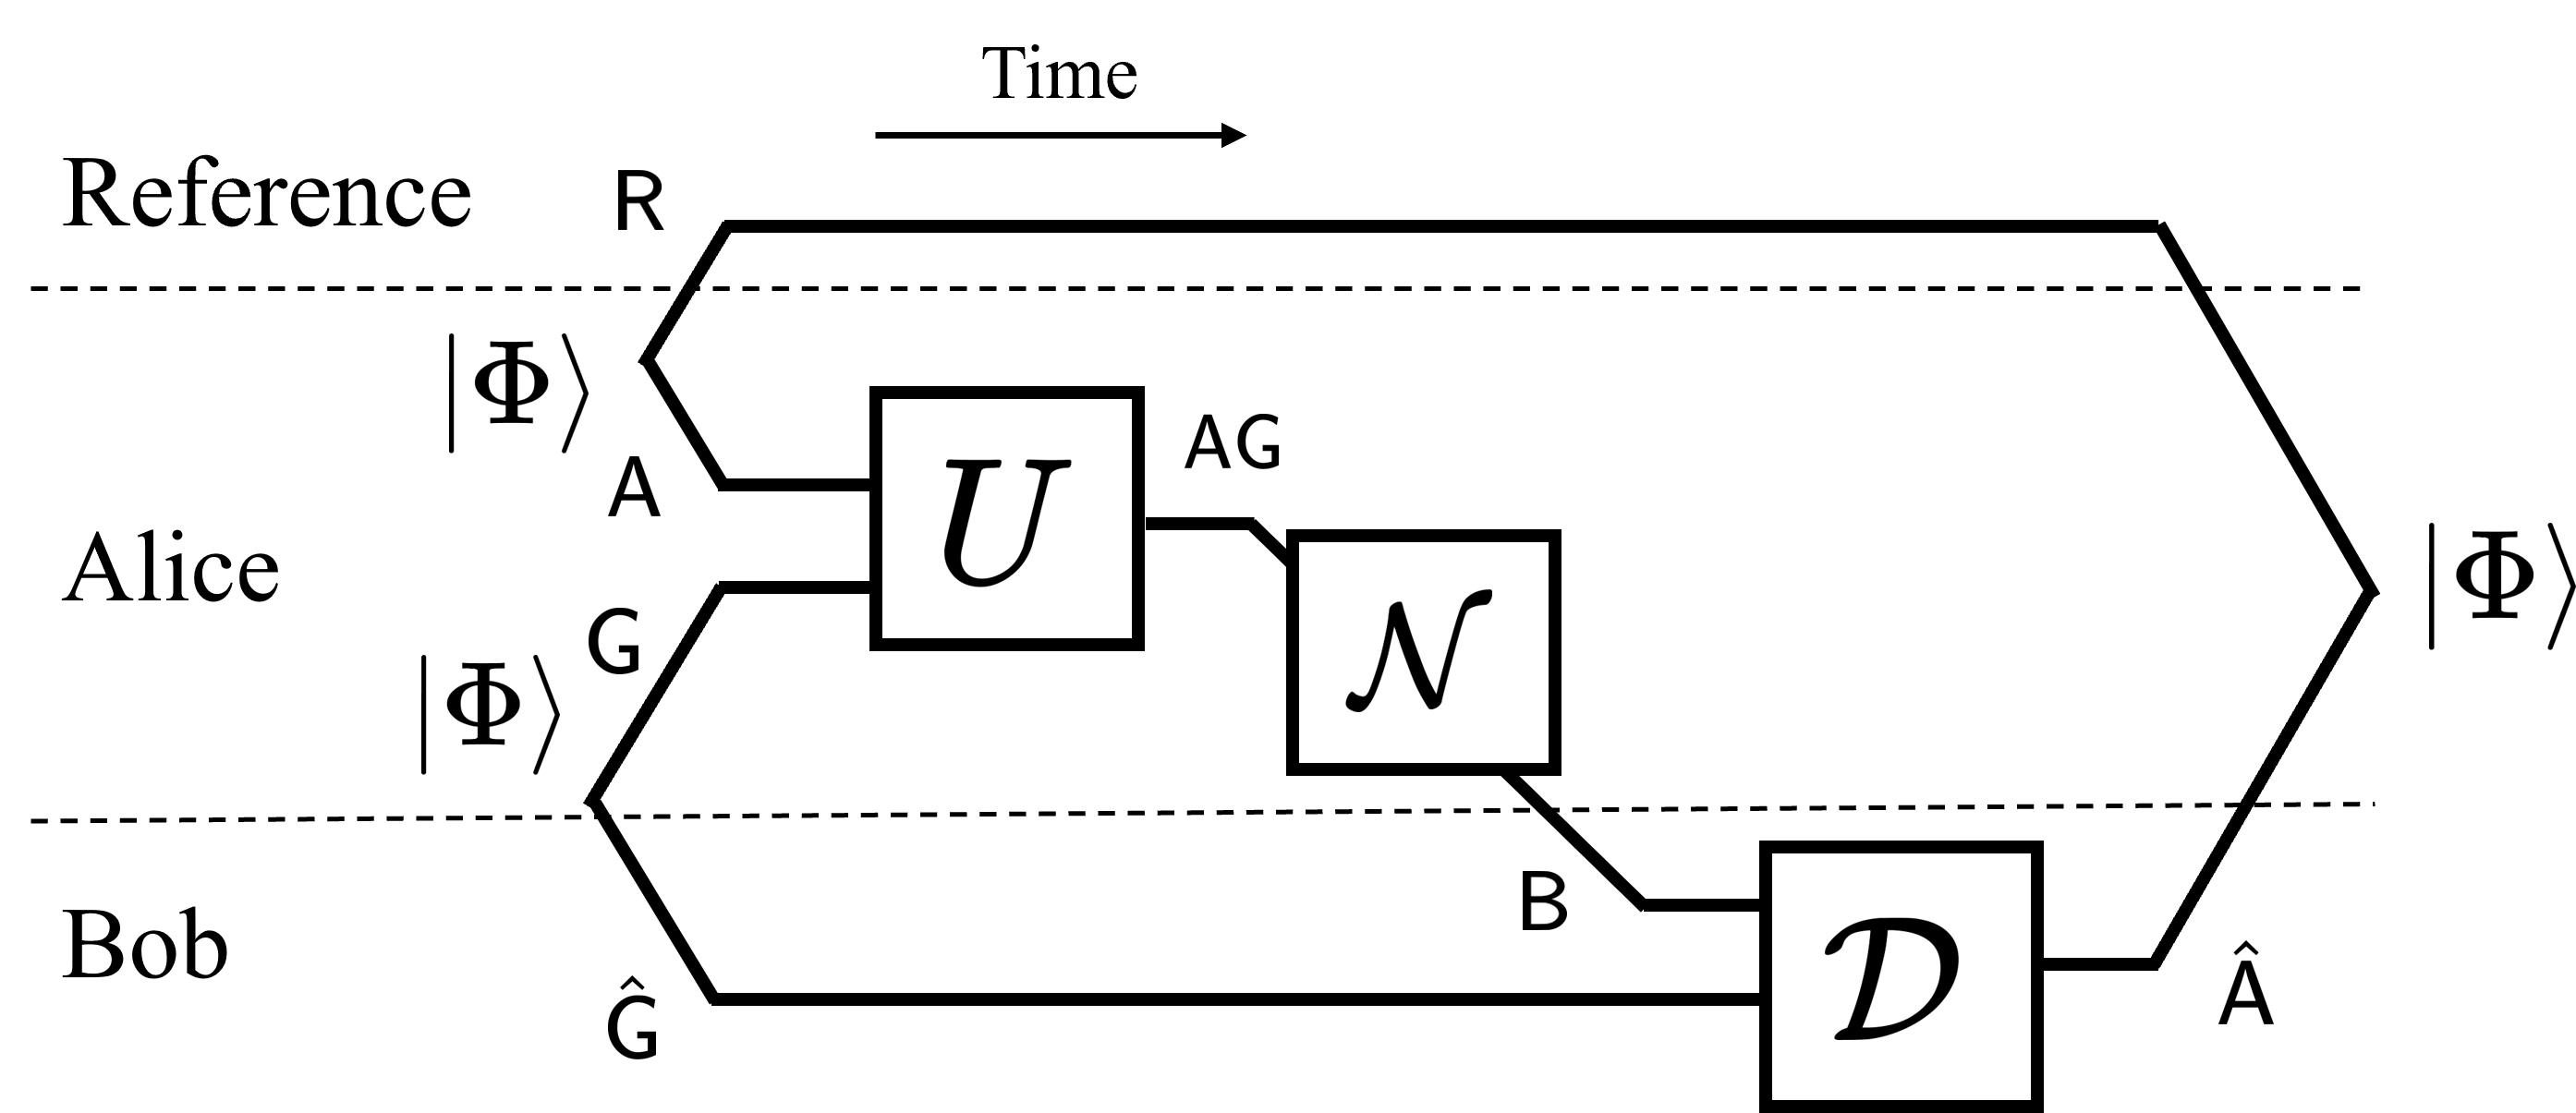
\includegraphics[width=100mm]{fig3.png}
    \caption{A diagram of entanglement transmission. 
    Alice applies a Haar random unitary $U^{\sA\sG}$ to encode $\sA$ with $\sG$, which is part of a possibly pre-shared entangled state $\ket{\Phi}^{\sG\hat{\sG}}$. Alice then transmits $\sA\sG$ to Bob through a noisy quantum channel $\cN^{\sA\sG\rarr\sB}$.
    After receiving $\sB$, Bob applies a decoding map $\cD^{\sB\hat{\sG}\rarr\hat{\sA}}$ on $\sB\hat{\sG}$ to obtain a final state that approximates the maximally entangled state $\ket{\Phi}^{\sR\hat{\sA}}$.}
    \label{fig:diagram of QI transmitt}
\end{figure}





%=====================================================================================================================================================================================================================================


\subsubsection{Algorithmic implementation of the Uhlmann decoder}
\label{sec:analyze of uhl alg in ent trans}


We consider that Bob implements the Uhlmann decoder using our algorithm.
We assume that Bob knows Alice's operation $U^{\sA\sG}$ and is capable of applying it.
It is standard in decoding to assume that Bob knows how Alice encoded the system.
Even if $U^{\sA\sG}$ is chosen uniformly at random, Bob can determine which unitary was applied, for example, using shared randomness with Alice.
Let $U_\cN^{\sS}$ be a Stinespring unitary on $\sS = \sA\sG\sC = \sB\sE$, i.e., $U_\cN^{\sS}\ket{0}^{\sC} = V_\cN^{\sA\sG\rarr\sB\sE}$, where $V_\cN^{\sA \to \sB\sE}$ is a Stinespring isometry of $\cN^{\sA \to \sB}$.
For algorithmic construction, we consider two different models: 
\begin{enumerate}
    \item A model in which multiple uses of a Stinespring unitary $U_\cN^{\sS'}$ are available.
    \item A model in which multiple uses of the quantum channel $\cN^{\sA'\sG' \to \sB'}$ are available.
\end{enumerate}
We evaluate the number of uses of $U_\cN^{\sS'}$ or $\cN^{\sA'\sG'\rarr\sB'}$ by Bob to implement the Uhlmann decoder in each model.
Note that we should distinguish between the existing systems, such as $\sR$ and $\sS$, and the systems subsequently prepared and simulated by Bob, e.g., $\sS'$.





We define two pure states $\ket{\Psi}^{\sR\sB\hat{\sG}\sE}$ and $\ket{\tau}^{\sR\sB\hat{\sG}\sE}$ as 
\begin{align}
    \ket{\Psi}^{\sR\sB\hat{\sG}\sE} = V_\cN^{\sA\sG\rarr\sB\sE} U^{\sA\sG} \ket{\Phi}^{\sR\sA}\ket{\Phi}^{\sG\hat{\sG}}, \ \ \ \text{and} \ \ \
    \ket{\tau}^{\sR\sB\hat{\sG}\sE} = V_\cN^{\sA\sG\rarr\sB\sE}\ket{\Phi}^{\sR\sA}\ket{\Phi}^{\sG\hat{\sG}}.
\end{align}
For a matrix $A$, we use $\lambda_{\rm min}(A)$ and $r(A)$ to denote the minimum non-zero eigenvalue and the rank of $A$, respectively.
Our statement is as follows, where $\mu_{\rm min}$ is given by $\mu_{\rm min} = \sqrt{\lambda_{\rm min}(\Psi^{\sB\hat{\sG}})\lambda_{\rm min}(\tau^{\sB\hat{\sG}})/d_\sA}$.

\begin{theorem}[Algorithmic implementation of the Uhlmann decoder]
\label{thm:Uhlmann decoder ent trans}
    In the setting of entanglement transmission, suppose that an encoding unitary $U^{\sA\sG}$ satisfies
    \begin{align}
    \label{inteq:136}
        \rF\big(\bar{\cN}^{\sA\sG\rarr\sE}\circ\cU^{\sA\sG}(\Phi^{\sR\sA} \otimes \pi^\sG), \pi^\sR \otimes \tau^\sE\big) \geq 1 - \epsilon,
    \end{align}
    for some $\epsilon \in [0, 1]$ and $\tau^\sE = \bar{\cN}^{\sA\sG\rarr\sE}(\pi^{\sA\sG})$.
    Then, for $\delta \in (0, 1)$, there exists a quantum algorithm that implements a quantum channel $\til{\cD}^{\sB\hat{\sG}\rarr\hat{\sA}}$, which satisfies
    \begin{align}
    \label{inteq:157}
        \rF\big(\til{\cD}^{\sB\hat{\sG} \rarr \hat{\sA}}(\Psi^{\sR\sB\hat{\sG}}), \ket{\Phi}^{\sR\hat{\sA}}\big) \geq 1 - \epsilon -\delta,
    \end{align}
    using, in Model~1: 
    \begin{align}
    \label{inteq:121}
        \cO\Big(\min\Big\{\f{1}{\mu_{\rm min}}, \f{r(\Psi^{\sB\hat{\sG}})}{\delta}\Big\}\log{\Big(\f{1}{\delta}\Big)}\Big)
    \end{align}
    of a Stinespring unitary $U_\cN^{\sS'}$ or, 
    in Model~2: 
    \begin{align}
    \label{inteq:137}
        \til{\cO}\Big(\f{d_\sA d_\sB d_\sG}{\delta^2 \mu_{\rm min}^3} \min\Big\{\f{1}{\lambda_{\rm min}^2(\Psi^{\sR\sB\hat{\sG}})} + \f{1}{\lambda_{\rm min}^2(\tau^{\sR\sB\hat{\sG}})}, \f{d_\sA^2 d_\sB^2 d_\sG^2}{\delta^4 \mu_{\rm min}^4}\Big\}\Big)
    \end{align}
    of the quantum channel $\cN^{\sA'\sG'\rarr\sB'}$.
    In both models, $\cO\big(\log{(d_\sA d_\sB d_\sG)}\big)$ qubits suffice at any one time.
\end{theorem}



In each model, if one is interested in the circuit complexity, it can be estimated to the leading order by multiplying the number of one- and two-qubit gates for implementing $U_\cN^{\sS'}$ or $\cN^{\sA'\sG'\rarr\sB'}$ by the respective number of times they are used, given in Eq.~\eqref{inteq:121} and Eq.~\eqref{inteq:137}.



Before proceeding to the proof of Theorem~\ref{thm:Uhlmann decoder ent trans}, we briefly compare the number of uses of $U_\cN^{\sS'}$ in Eq.~\eqref{inteq:121} with those of existing decoders, the generalized Yoshida-Kitaev decoder, and the Petz-like decoder~\cite{utsumi2024explicitdecoderQSVTt}.
The number of uses of $U_\cN^{\sS'}$ in these decoders is given by
\begin{align}
\label{inteq:82}
    \cO\Big(\sqrt{d_\sB/\big(d_\sG\lambda_{\rm min}(\Psi^{\sB\hat{\sG}})\big)}\log{(1/\delta)}\Big),
\end{align}
for the generalized Yoshida-Kitaev decoder, and
\begin{align}
\label{inteq:83}
    \cO\Big(\sqrt{d_\sE/\big(d_\sA\lambda_{\rm min}(\Psi^{\sB\hat{\sG}})\big)} \log{(1/\delta)}\Big),
\end{align}
for the Petz-like decoder.
From the comparison of Eqs.~\eqref{inteq:121} and~\eqref{inteq:82}, we see that if an inequality 
\begin{align}
    \f{d_\sG}{d_\sB}\min\Big\{\f{d_\sA}{\lambda_{\rm min}(\tau^{\sB\hat{\sG}})}, \f{1}{\delta^2}\Big\} \leq 1,
\end{align}
is satisfied, the Uhlmann decoder can be implemented more efficiently than the generalized Yoshida-Kitaev one, where we used the relation $r(\Psi^{\sB\hat{\sG}}) \leq 1/\lambda_{\rm min}(\Psi^{\sB\hat{\sG}})$.
Similarly, comparing Eqs.~\eqref{inteq:121} and~\eqref{inteq:83}, we observe that when $\f{d_\sE}{d_\sA}\min\Big\{\f{d_\sA}{\lambda_{\rm min}(\tau^{\sB\hat{\sG}})}, \f{1}{\delta^2}\Big\} \leq 1$, the Uhlmann decoder can be implemented more efficiently than the Petz-like decoder.









\begin{proof}[Proof of Theorem~\ref{thm:Uhlmann decoder ent trans}]
    

We first consider Model~1.


We note that the states $\ket{\Psi}^{\sR\sB\hat{\sG}\sE}\ket{0}^{\hat{\sR}\hat{\sA}}$ and $\ket{\Phi}^{\sR\hat{\sA}}\ket{\tau}^{\hat{\sR}\sB\hat{\sG}\sE}$ are rephrased as 
$\ket{\Psi}^{\sR\sB\hat{\sG}\sE}\ket{0}^{\hat{\sR}\hat{\sA}} = W_\cN^{\sR\sS\hat{\sG}\hat{\sR}\hat{\sA}}\ket{0}^{\sR\sS\hat{\sG}\hat{\sR}\hat{\sA}}$ and $\ket{\Phi}^{\sR\hat{\sA}}\ket{\tau}^{\hat{\sR}\sB\hat{\sG}\sE} = \til{W}_\cN^{\sR\sS\hat{\sG}\hat{\sR}\hat{\sA}}\ket{0}^{\sR\sS\hat{\sG}\hat{\sR}\hat{\sA}}$, where
\begin{align}
    W_\cN^{\sR\sS\hat{\sG}\hat{\sR}\hat{\sA}} = U_\cN^{\sS}U^{\sA\sG}(U_\Phi^{\sR\sA}\otimes U_\Phi^{\sG\hat{\sG}})\otimes \bI^{\hat{\sR}\hat{\sA}}, \ \ \text{and} \ \ \ 
    \til{W}_\cN^{\sR\sS\hat{\sG}\hat{\sR}\hat{\sA}} = U_\Phi^{\sR\hat{\sA}} \otimes U_\cN^{\sS}(U_\Phi^{\hat{\sR}\sA}\otimes U_\Phi^{\sG\hat{\sG}}),
\end{align}
$U_\Phi\ket{0} = \ket{\Phi}$, and $\sS = \sA\sG\sC = \sB\sE$.
Using
\begin{align}
    \mathtt{UhlmannPurifiedQuery}(W_\cN^{\sR'\sS'\hat{\sG}'\hat{\sR}'\hat{\sA}'}, \til{W}_\cN^{\sR'\sS'\hat{\sG}'\hat{\sR}'\hat{\sA}'}; \delta, \tF),
\end{align}
described in \Cref{alg:Uhl purif query}, we can implement a quantum channel $\cT^\sM$ on $\sM = \sB\hat{\sG}\hat{\sR}\hat{\sA}$, which approximates the Uhlmann transformation and satisfies
\begin{align}
    \rF\big(\cT^\sM(\ketbra{\Psi}{\Psi}^{\sR\sB\hat{\sG}\sE}\otimes\ketbra{0}{0}^{\hat{\sR}\hat{\sA}}), \ket{\Phi}^{\sR\hat{\sA}}\ket{\tau}^{\hat{\sR}\sB\hat{\sG}\sE}\big)
    &\geq \rF(\Psi^{\sR\sE}, \pi^\sR\otimes\tau^\sE) -\delta \\
    &\geq 1-\epsilon - \delta,
\end{align}
where we used Theorem~\ref{thm:Uhlmann alg purif query model} and the decoupling condition Eq.~\eqref{inteq:136}.
Note that $\Psi^{\sR\sE} = \bar{\cN}^{\sA\sG\rarr\sE}\circ\cU^{\sA\sG}(\Phi^{\sR\sA} \otimes \pi^\sG)$.
From the monotonicity of the fidelity, a quantum channel $\til{\cD}^{\sB\hat{\sG}\rarr\hat{\sA}} = \tr_{\sB\hat{\sG}\hat{\sR}}\circ\cT^\sM \circ \cP_{\ket{0}}^{\bC\rarr\hat{\sR}\hat{\sA}}$ serves as a decoder such that
\begin{align}
    &\rF(\til{\cD}^{\sB\hat{\sG}\rarr\hat{\sA}}(\Psi^{\sR\sB\sG}), \ket{\Phi}^{\sR\hat{\sA}}) 
    \geq 1 - \epsilon - \delta.
\end{align}


The number of uses of $U_\cN^{\sS'}$ for applying the channel $\til{\cD}^{\sB\hat{\sG}\rarr\hat{\sA}}$, especially $\cT^\sM$, can be evaluated by Theorem~\ref{thm:Uhlmann alg purif query model} as
\begin{align}
\label{inteq:81}
    \cO\big(\min\{{1/s_{\rm min}}, r/\delta\}\log{(1/\delta)}\big), 
\end{align}
where $s_{\rm min}$ and $r$ are the minimum non-zero singular value and the rank of $\sqrt{\Psi^{\sR\sE}}\big(\sqrt{\pi^\sR}\otimes\sqrt{\tau^\sE}\big)$, respectively.

By applying the following two inequalities:
\begin{align}
    \label{inteq:138}
    &1/s_{\rm min} \leq \sqrt{d_\sA/\big(\lambda_{\rm min}(\Psi^{\sB\hat{\sG}})\lambda_{\rm min}(\tau^{\sB\hat{\sG}})\big)} = 1/\mu_{\rm min},  \\
    \label{inteq:139}
    &r \leq r(\Psi^{\sB\hat{\sG}}),
\end{align}
to Eq.~\eqref{inteq:81}, we finally obtain Eq.~\eqref{inteq:121}.
The inequalities follow from the so-called support lemma~\cite{Renner05securityQKD, wilde2013QItheory}: for any positive-semidefinite matrix $S^{\sA\sB}$, $\supp[S^{\sA\sB}] \subset \supp[S^\sA\otimes S^\sB]$.
By combining this fact with \Cref{prop:min singular inequality} in \Cref{sec:appendix product of singvalue}, Eq.~\eqref{inteq:138} is obtained.
Here, we note that $\tr_\sE[\Psi^{\sR\sE}] = \pi^\sR$ and $\tr_\sR[\Psi^{\sR\sE}] = \tau^\sE$.
The inequality in Eq.~\eqref{inteq:139} results from the rank of a product of matrices being at most the rank of each matrix.
Since $\supp[\Psi^{\sR\sE}] \subset \supp[\pi^\sR \otimes \tau^\sE]$, we have $\min\{r(\Psi^{\sR\sE}), r(\pi^\sR\otimes \tau^\sE)\} = r(\Psi^{\sR\sE})$.
Note that $\ket{\Psi}^{\sR\sB\hat{\sG}\sE}$ is a pure state, which implies $r(\Psi^{\sR\sE}) = r(\Psi^{\sB\hat{\sG}})$.







Next, we consider Model~2.
In this model, we need to obtain purified states, using a purification algorithm such as the canonical purification algorithm in \Cref{alg:canonical purification}.
Since the input state to the decoder does not depend on the choice of the environment $\sE$, for canonical purification, we set $\sE$ as $\sE = \sR''\sB''\hat{\sG}''$.




In contrast to Model~1, the construction of a decoder in Model~2 requires careful analysis, because considering a specific purification fixes the freedom in the environment of the channel $\cN^{\sA\sG\rarr\sB}$.
We explain the issue and its resolution below. 




The canonical purified states of
\begin{align}
\label{inteq:11}
    \Psi^{\sR\sB\hat{\sG}} = \cN^{\sA\sG\rarr\sB}\circ\cU^{\sA\sG}(\Phi^{\sR\sA}\otimes\Phi^{\sG\hat{\sG}}), \ \ \ \text{and} \ \ \ \tau^{\sR\sB\hat{\sG}} = \cN^{\sA\sG\rarr\sB}(\Phi^{\sR\sA}\otimes\Phi^{\sG\hat{\sG}}),
\end{align}
are given by 
\begin{align}
    &\ket{\Psi_{\rm c}}^{\sR\sB\hat{\sG}\sR''\sB''\hat{\sG}''} = \sqrt{\Psi^{\sR\sB\hat{\sG}}}\ket{\Gamma}^{\sR\sB\hat{\sG}\sR''\sB''\hat{\sG}''}, \label{Eq:PsiCanonical} \\
    &\ket{\tau_{\rm c}}^{\sR\sB\hat{\sG}\sR''\sB''\hat{\sG}''} = \sqrt{\tau^{\sR\sB\hat{\sG}}}\ket{\Gamma}^{\sR\sB\hat{\sG}\sR''\sB''\hat{\sG}''},
\end{align}
respectively, where $\ket{\Gamma}^{\sR\sB\hat{\sG}\sR''\sB''\hat{\sG}''}$ is the unnormalized maximally entangled state between $\sR\sB\hat{\sG}$ and $\sR''\sB''\hat{\sG}''$.
The Stinespring isometry $V_{\cN, \tau_{\rm c}}^{\sA\sG\rarr\sB\sR''\sB''\hat{\sG}''}$ of $\cN^{\sA\sG\rarr\sB}$, determined from $\ket{\tau_{\rm c}}^{\sR\sB\hat{\sG}\sR''\sB''\hat{\sG}''}$, satisfies
\begin{align}
\label{inteq:66}
    \ket{\tau_{\rm c}}^{\sR\sB\hat{\sG}\sR''\sB''\hat{\sG}''} 
    = V_{\cN, \tau_{\rm c}}^{\sA\sG\rarr\sB\sR''\sB''\hat{\sG}''}\ket{\Phi}^{\sR\sA}\ket{\Phi}^{\sG\hat{\sG}}.
\end{align}



To see how $V_{\cN, \tau_{\rm c}}^{\sA\sG\rarr\sB\sR''\sB''\hat{\sG}''}$ is related to the Stinespring isometry determined from $\ket{\Psi_{\rm c}}^{\sR\sB\hat{\sG}\sR''\sB''\hat{\sG}''}$, we note that Eqs.~\eqref{inteq:11} imply $\Psi^{\sR\sB\hat{\sG}} = (U^{\sR\hat{\sG}})^\top\tau^{\sR\sB\hat{\sG}}(U^{\sR\hat{\sG}})^*$, where we used the property of the maximally entangled state: $U^\sA\ket{\Phi}^{\sA\sA'} = (U^{\sA'})^\top\ket{\Phi}^{\sA\sA'}$.
Substituting this into Eq.~\eqref{Eq:PsiCanonical} and, again, using the property of the maximally entangled state, the canonical purified state $\ket{\Psi_{\rm c}}^{\sR\sB\hat{\sG}\sR''\sB''\hat{\sG}''}$ can be written as
\begin{align}
    \ket{\Psi_{\rm c}}^{\sR\sB\hat{\sG}\sR''\sB''\hat{\sG}''}
    &= \big((U^{\sR\hat{\sG}})^\top\otimes(U^{\sR''\hat{\sG}''})^\dag\big)\ket{\tau_{\rm c}}^{\sR\sB\hat{\sG}\sR''\sB''\hat{\sG}''} \\
    \label{inteq:132}
    &=(U^{\sR''\hat{\sG}''})^\dag V_{\cN, \tau_{\rm c}}^{\sA\sG\rarr\sB\sR''\sB''\hat{\sG}''} U^{\sA\sG}\ket{\Phi}^{\sR\sA}\ket{\Phi}^{\sG\hat{\sG}}.
\end{align}
Hence, the Stinespring isometry $V_{\cN, \Psi_{\rm c}}^{\sA\sG\rarr\sB\sR''\sB''\hat{\sG}''}$ of $\cN^{\sA\sG\rarr\sB}$, determined from $\ket{\Psi_{\rm c}}^{\sR\sB\hat{\sG}\sR''\sB''\hat{\sG}''}$, is given by 
\begin{align}
\label{inteq:154}
    V_{\cN, \Psi_{\rm c}}^{\sA\sG\rarr\sB\sR''\sB''\hat{\sG}''} = (U^{\sR''\hat{\sG}''})^\dag V_{\cN, \tau_{\rm c}}^{\sA\sG\rarr\sB\sR''\sB''\hat{\sG}''}.
\end{align}
As a result, the complementary channels of $\cN^{\sA\sG\rarr\sB}$ induced by each of $V_{\cN, \tau_{\rm c}}^{\sA\sG\rarr\sB\sR''\sB''\hat{\sG}''}$ and $V_{\cN, \Psi_{\rm c}}^{\sA\sG\rarr\sB\sR''\sB''\hat{\sG}''}$ are generally not identical: $\bar{\cN}_{\tau_{\rm c}}^{\sA\sG\rarr\sR''\sB''\hat{\sG}''} \neq \bar{\cN}_{\Psi_{\rm c}}^{\sA\sG\rarr\sR''\sB''\hat{\sG}''}$, where $\bar{\cN}_\omega^{\sA\sG\rarr\sR''\sB''\hat{\sG}''}$ is given by $\bar{\cN}_\omega^{\sA\sG\rarr\sR''\sB''\hat{\sG}''}(\cdot) = \tr_\sB\big[V_{\cN, \omega}^{\sA\sG\rarr\sB\sR''\sB''\hat{\sG}''}(\cdot)\big(V_{\cN, \omega}^{\sA\sG\rarr\sB\sR''\sB''\hat{\sG}''}\big)^\dag\big]$
for $\omega = \tau_{\rm c}, \Psi_{\rm c}$.





This mismatch of the complementary channels prevents a straightforward application of the decoupling condition Eq.~\eqref{inteq:136} when we construct the Uhlmann transformation $V^\sM$ on $\sM = \sB\hat{\sG}\hat{\sR}\hat{\sA}$ from the canonical purifications $\ket{\Psi_{\rm c}}^{\sR\sB\hat{\sG}\sR''\sB''\hat{\sG}''}$ and $\ket{\tau_{\rm c}}^{\sR\sB\hat{\sG}\sR''\sB''\hat{\sG}''}$.
In fact, this Uhlmann transformation $V^\sM$ satisfies  
\begin{align}
    &\rF\big(V^\sM\ket{\Psi_{\rm c}}^{\sR\sB\hat{\sG}\sR''\sB''\hat{\sG}''}\ket{0}^{\hat{\sR}\hat{\sA}}, \ket{\Phi}^{\sR\hat{\sA}}\ket{\tau_{\rm c}}^{\hat{\sR}\sB\hat{\sG}\sR''\sB''\hat{\sG}''}\big) \notag \\
    \label{inteq:156}
    &= \rF\big(\bar{\cN}_{\Psi_{\rm c}}^{\sA\sG\rarr\sR''\sB''\hat{\sG}''}\circ\cU^{\sA\sG}(\Phi^{\sR\sA} \otimes \pi^\sG), \pi^\sR\otimes\bar{\cN}_{\tau_{\rm c}}^{\sA\sG\rarr\sR''\sB''\hat{\sG}''}(\pi^{\sA\sG})\big). 
\end{align}
However, this fidelity is not necessarily close to one even under the assumption of the decoupling condition Eq.~\eqref{inteq:136}.
This is simply because
the right-hand side of Eq.~\eqref{inteq:156} involves two different complementary channels $\bar{\cN}_{\Psi_{\rm c}}^{\sA\sG\rarr\sR''\sB''\hat{\sG}''}$ and $\bar{\cN}_{\tau_{\rm c}}^{\sA\sG\rarr\sR''\sB''\hat{\sG}''}$.



From the decoupling condition Eq.~\eqref{inteq:136}, we can conclude that the fidelity in the right-hand side in Eq.~\eqref{inteq:156} is $\epsilon$-close to one only if the two complementary channels coincide, which is in general not the case.
Therefore, the Uhlmann transformation constructed from $\ket{\Psi_{\rm c}}^{\sR\sB\hat{\sG}\sR''\sB''\hat{\sG}''}$ and $\ket{\tau_{\rm c}}^{\sR\sB\hat{\sG}\sR''\sB''\hat{\sG}''}$ does not serve as a proper decoder.
Below, we describe a procedure to resolve this issue.




The issue that the complementary channels from $\ket{\Psi_{\rm c}}^{\sR\sB\hat{\sG}\sR''\sB''\hat{\sG}''}$ and $\ket{\tau_{\rm c}}^{\sR\sB\hat{\sG}\sR''\sB''\hat{\sG}''}$ generally differ can be resolved if Bob applies the encoding unitary to the system $\sR''\hat{\sG}''$ of the copies of $\ket{\Psi_{\rm c}}^{\sR\sB\hat{\sG}\sR''\sB''\hat{\sG}''}$.
From Eq.~\eqref{inteq:154}, we observe that an extra unitary $(U^{\sR''\hat{\sG}''})^\dag$ appears, which obstructs the direct application of the decoupling condition.
By additionally applying $U^{\sR''\hat{\sG}''}$ to the copies of $\ket{\Psi_{\rm c}}^{\sR\sB\hat{\sG}\sR''\sB''\hat{\sG}''}$ held by Bob, the extra unitary is canceled.
See also Fig.~\ref{fig:dilation states}.



\begin{figure}
    \centering
    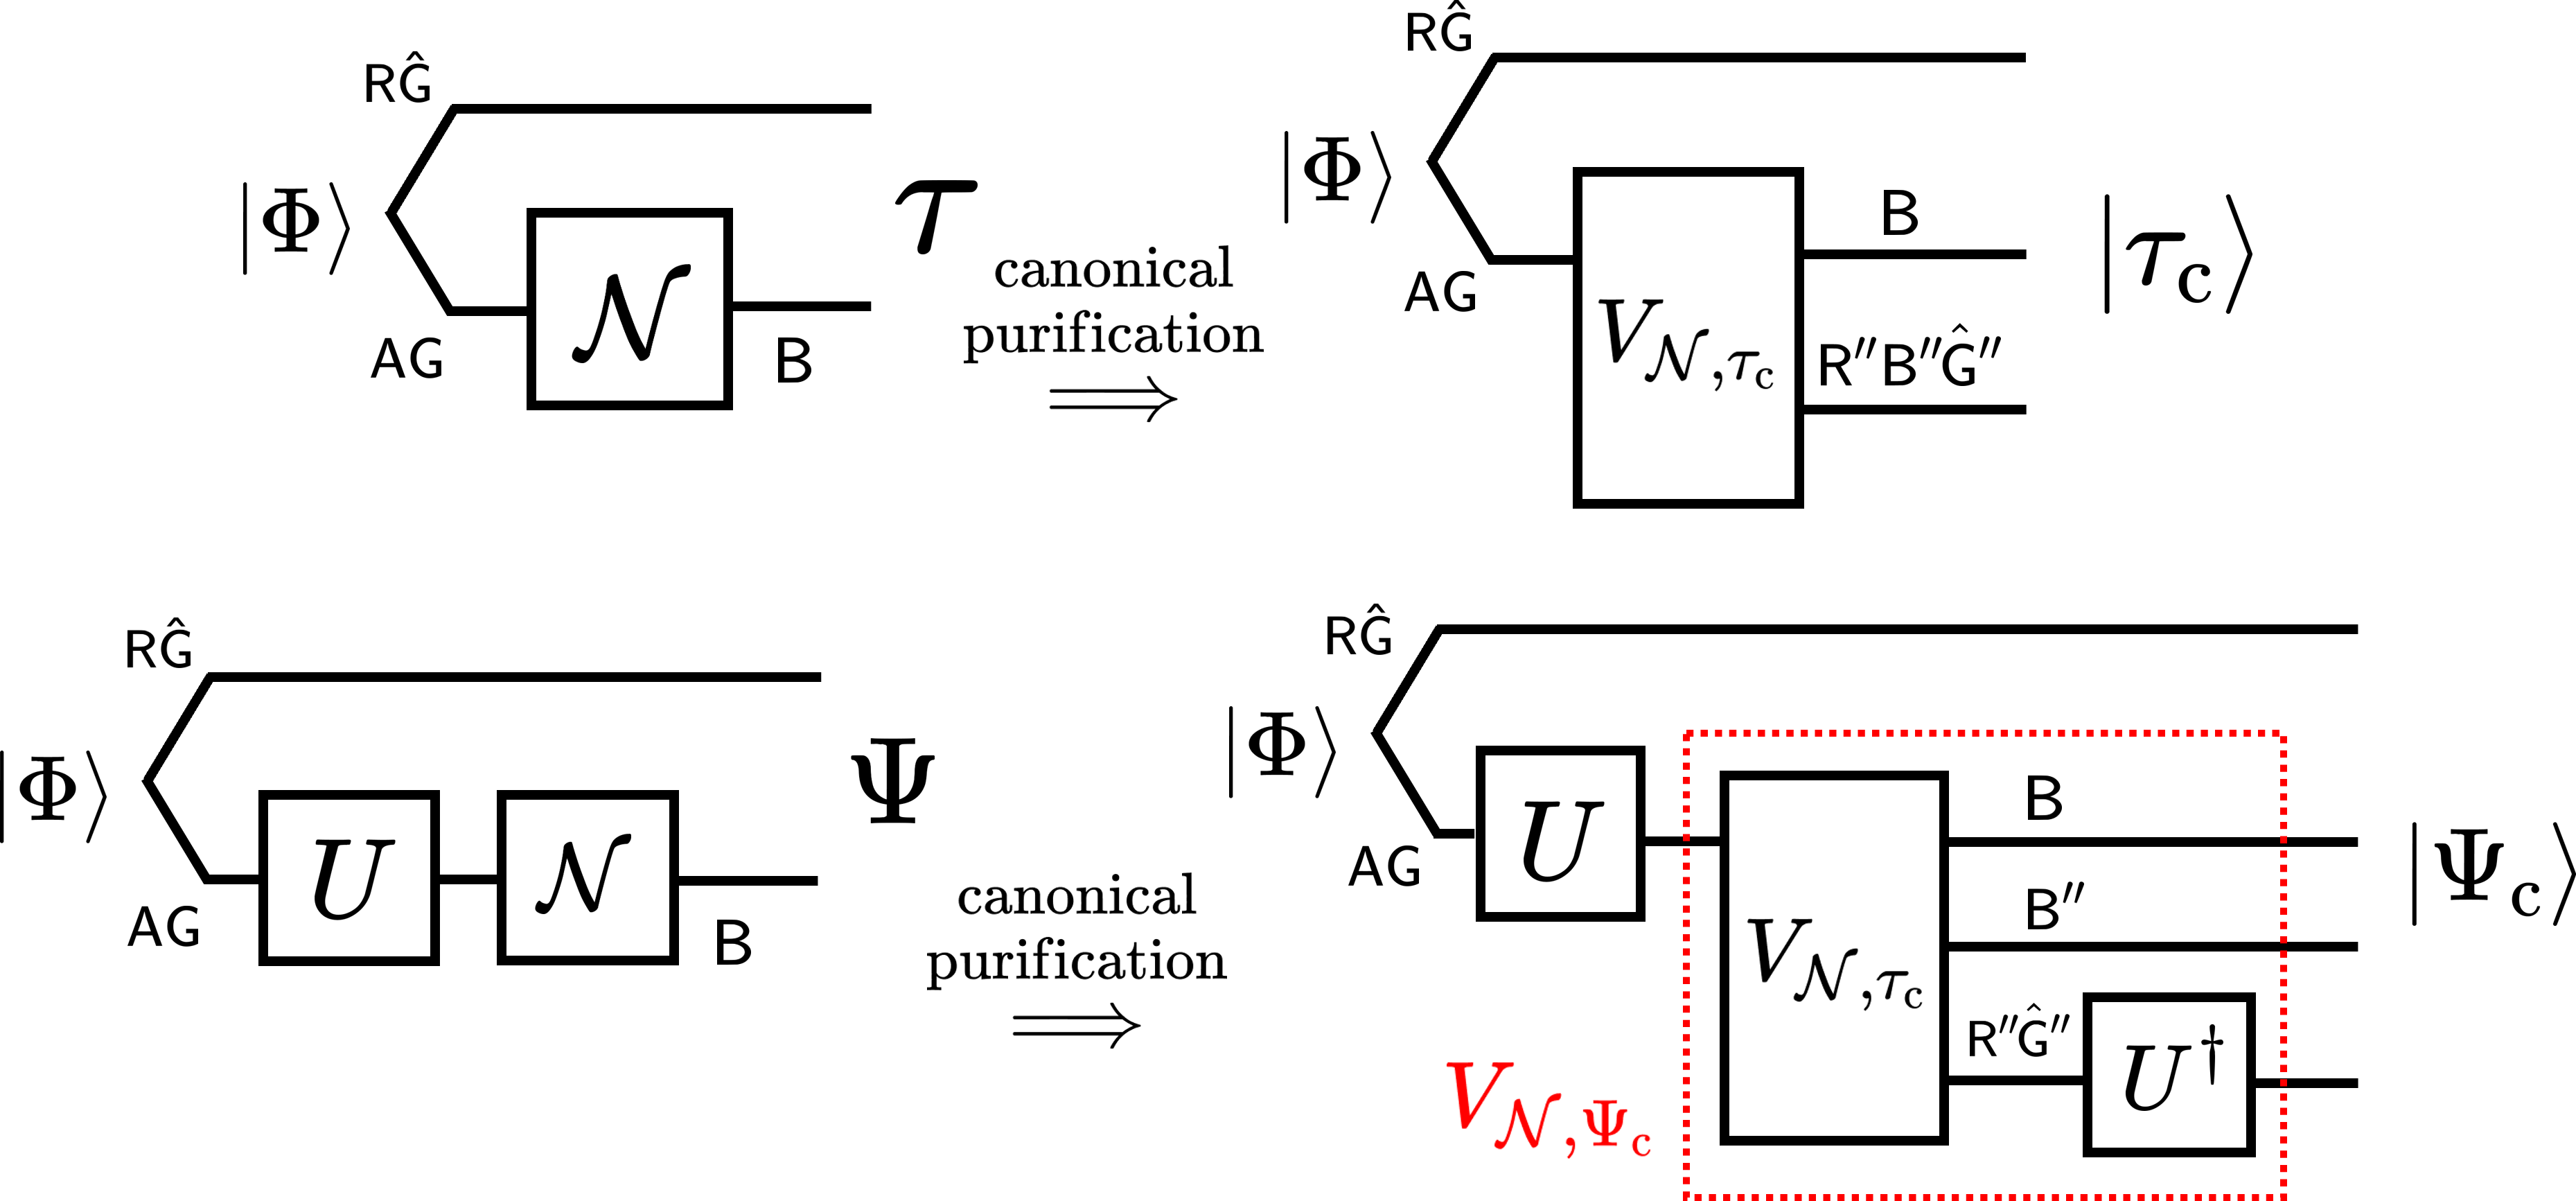
\includegraphics[width=120mm]{fig6.png}
    \caption{A diagram of the Stinespring dilation of $\cN^{\sA\sG\rarr\sB}$ induced by the canonical purification.
    We denote by $V_{\cN, \tau_{\rm c}}^{\sA\sG\rarr\sB\sR''\sB''\hat{\sG}''}$ the Stinespring isometry associated with $\ket{\tau_{\rm c}}^{\sR\sB\hat{\sG}\sR''\sB''\hat{\sG}''}$.
    Then, the Stinespring isometry corresponding to $\ket{\Psi_{\rm c}}^{\sR\sB\hat{\sG}\sR''\sB''\hat{\sG}''}$ is given by $(U^{\sR''\hat{\sG}''})^\dag V_{\cN, \tau_{\rm c}}^{\sA\sG\rarr\sB\sR''\sB''\hat{\sG}''}$, which is denoted as $V_{\cN, \Psi_{\rm c}}^{\sA\sG\rarr\sB\sR''\sB''\hat{\sG}''}$ and shown in a red dotted box.
    The complementary channels determined from these isometries are generally not identical, so Eq.~\eqref{inteq:136} cannot be applied directly.
    To resolve this issue, it suffices for Bob to apply $U^{\sR''\hat{\sG}''}$ to copies of $\ket{\Psi_{\rm c}}^{\sR\sB\hat{\sG}\sR''\sB''\hat{\sG}''}$ at hand in the algorithm, thereby canceling the extra $(U^{\sR''\hat{\sG}''})^\dag$.}
    \label{fig:dilation states}
\end{figure}



Let $\ket{\til{\Psi}_{\rm c}}^{\sR\sB\hat{\sG}\sR''\sB''\hat{\sG}''}$ be a state given by $\ket{\til{\Psi}_{\rm c}}^{\sR\sB\hat{\sG}\sR''\sB''\hat{\sG}''} = U^{\sR''\hat{\sG}''}\ket{\Psi_{\rm c}}^{\sR\sB\hat{\sG}\sR''\sB''\hat{\sG}''}$. One can check that the complementary channels associated with $\ket{\til{\Psi}_{\rm c}}^{\sR\sB\hat{\sG}\sR''\sB''\hat{\sG}''}$ and $\ket{\tau_{\rm c}}^{\sR\sB\hat{\sG}\sR''\sB''\hat{\sG}''}$ are identical: $\bar{\cN}_{\tau_{\rm c}}^{\sA\sG\rarr\sR''\sB''\hat{\sG}''} = \bar{\cN}_{\til{\Psi}_{\rm c}}^{\sA\sG\rarr\sR''\sB''\hat{\sG}''}$. We denote these channel by $\bar{\cN}_{\rm c}^{\sA\sG\rarr\sR''\sB''\hat{\sG}''}$ for simplicity.
When we construct the Uhlmann transformation $\til{V}^\sM$ from $\ket{\til{\Psi}_{\rm c}}^{\sR\sB\hat{\sG}\sR''\sB''\hat{\sG}''}$ and $\ket{\tau_{\rm c}}^{\sR\sB\hat{\sG}\sR''\sB''\hat{\sG}''}$, it holds that
\begin{align}
\label{inteq:68}
    \rF\big(\til{V}^\sM\ket{\til{\Psi}_{\rm c}}^{\sR\sB\hat{\sG}\sR''\sB''\hat{\sG}''}\ket{0}^{\hat{\sR}\hat{\sA}}, \ket{\Phi}^{\sR\hat{\sA}}\ket{\tau_{\rm c}}^{\hat{\sR}\sB\hat{\sG}\sR''\sB''\hat{\sG}''}\big)
    &= \rF\big(\bar{\cN}_{\rm c}^{\sA\sG\rarr\sR''\sB''\hat{\sG}''}\circ\cU^{\sA\sG}(\Phi^{\sR\sA} \otimes \pi^\sG), \pi^\sR\otimes \tau_{\rm c}^{\sR''\sB''\hat{\sG}''}\big) \\
    &\geq 1 -\epsilon,
\end{align}
where $\tau_{\rm c}^{\sR''\sB''\hat{\sG}''} = \bar{\cN}_{\rm c}^{\sA\sG\rarr\sR''\sB''\hat{\sG}''}(\pi^{\sA\sG})$.
The inequality is due to the decoupling condition Eq.~\eqref{inteq:136}, where $\sE = \sR''\sB''\hat{\sG}''$.
While Bob cannot act on $\sR''\hat{\sG}''$ of the \emph{actual} environment, rather than on its copies, this does not cause any issue because the environment can be arbitrarily chosen.
Note that Eq.~\eqref{inteq:136} does not depend on the particular choice of the complementary channel of $\cN^{\sA\sG\rarr\sB}$, as long as the complementary channels appearing in the first and second arguments of the fidelity on the left-hand side are identical.




Based on the above discussion, to implement the Uhlmann decoder in this model, we introduce the following two simple modifications to
Algorithm~\ref{alg:Uhl mixed sample}, $\mathtt{UhlmannMixedSample}(\Psi^{\sR'\sB'\hat{\sG}'}, \tau^{\sR'\sB'\hat{\sG}'}; \delta, \tF)$.
The first modification is to apply an additional unitary $U^{\sR''\hat{\sG}''}$ after $\mathtt{CanonicalPurification}$ of $\Psi^{\sR'\sB'\hat{\sG}'}$.
The second modification is to perform the Uhlmann transformation on $\sM = \sB\hat{\sG}\hat{\sR}\hat{\sA}$ in the step of $\mathtt{UhlmannPurifiedSample}$, which approximately maps $\ket{\til{\Psi}_{\rm c}}^{\sR\sB\hat{\sG}\sR''\sB''\hat{\sG}''}\ket{0}^{\hat{\sR}\hat{\sA}}$ to $\ket{\Phi}^{\sR\hat{\sA}}\ket{\tau_{\rm c}}^{\hat{\sR}\sB\hat{\sG}\sR''\sB''\hat{\sG}''}$.
From Theorem~\ref{thm:Uhlmann mixed state sample}, we can implement a transformation $\cT^\sM$ that satisfies 
\begin{align}
    &\rF\big(\cT^\sM(\ketbra{\til{\Psi}_{\rm c}}{\til{\Psi}_{\rm c}}^{\sR\sB\hat{\sG}\sR''\sB''\hat{\sG}''}\otimes\ketbra{0}{0}^{\hat{\sR}\hat{\sA}}), \ket{\Phi}^{\sR\hat{\sA}}\ket{\tau_{\rm c}}^{\hat{\sR}\sB\hat{\sG}\sR''\sB''\hat{\sG}''}\big) \notag\\
    &\geq \rF\big(\bar{\cN}_{\rm c}^{\sA\sG\rarr\sR''\sB''\hat{\sG}''}\circ\cU^{\sA\sG}(\Phi^{\sR\sA} \otimes \pi^\sG), \pi^\sR\otimes \tau_{\rm c}^{\sR''\sB''\hat{\sG}''}\big) - \delta\\
    \label{inteq:161}
    &\geq 1 -\epsilon -\delta,
\end{align}
using multiple copies of $\Psi^{\sR'\sB'\hat{\sG}'}$ and $\tau^{\sR'\sB'\hat{\sG}'}$, where $\tau_{\rm c}^{\sR''\sB''\hat{\sG}''} = \bar{\cN}_{\rm c}^{\sA\sG\rarr\sR''\sB''\hat{\sG}''}(\pi^{\sA\sG})$ and we used the decoupling condition Eq.~\eqref{inteq:136}.
Hence, from Eq.~\eqref{inteq:161} and the monotonicity of the fidelity under the partial trace, we obtain that a quantum channel $\til{\cD}^{\sB\hat{\sG}\rarr\hat{\sA}}$ defined by $\til{\cD}^{\sB\hat{\sG} \rarr \hat{\sA}} = \tr_{\sB\hat{\sG}\hat{\sR}} \circ \cT^\sM \circ \cP_{\ket{0}}^{\bC\rarr\hat{\sR}\hat{\sA}}$ satisfies Eq.~\eqref{inteq:157}.



The number of uses of $\cN^{\sA'\sG'\rarr\sB'}$ for implementing $\til{\cD}^{\sB\hat{\sG}\rarr\hat{\sA}}$ is evaluated as
\begin{align}
\label{inteq:140}
    &\til{\cO}\Big(\f{d_\sA d_\sB d_\sG}{\delta^2 s_{\rm min}^3} \min\Big\{\f{1}{\lambda_{\rm min}^2(\Psi^{\sR\sB\hat{\sG}})} + \f{1}{\lambda_{\rm min}^2(\tau^{\sR\sB\hat{\sG}})}, \f{d_\sA^2 d_\sB^2 d_\sG^2}{\delta^4 s_{\rm min}^4}\Big\}\Big),
\end{align}
where $s_{\rm min}$ is the minimum non-zero singular value of $\sqrt{\til{\Psi}_{\rm c}^{\sR\sR''\sB''\hat{\sG}''}}\Big(\sqrt{\pi^\sR}\otimes\sqrt{\tau_{\rm c}^{\sR''\sB''\hat{\sG}''}}\Big)$.
Finally, applying Eq.~\eqref{inteq:138} to Eq.~\eqref{inteq:140}, we obtain the result of Eq.~\eqref{inteq:137}.
Since this algorithm runs sequentially in both Model~1 and Model~2, $\cO\big(\log(d_\sA d_\sB d_\sG)\big)$ qubits suffice at any one time.




\end{proof}







%==============================================================================================================================================





\subsection{One-shot quantum state merging}
\label{sec:entdis and uhl}

As another application of the decoupling and the Uhlmann transformation, we consider quantum state merging, which is often regarded as a generalization of entanglement distillation.
In \Cref{sec:setting of state merging}, we introduce the setting, and in \Cref{sec:implement uhl in state merging}, we discuss the implementation of the Uhlmann transformation for quantum state merging using our algorithm.


\subsubsection{Setting}
\label{sec:setting of state merging}


Suppose that a state $\ket{\omega}^{\sR\sA\sB}$ is shared between Alice, Bob, and the reference $\sR$, where $\sA$ and $\sB$ are held by Alice and Bob, respectively.
Their goal is to transfer Alice's system $\sA$ of $\ket{\omega}^{\sR\sA\sB}$ to Bob using only local operations and noiseless classical communication, while simultaneously distilling as much entanglement as possible between Alice and Bob.
That is, the task is to implement the following transformation, with the size of systems $\sS$ and $\hat{\sS}$ taken as large as possible:
\begin{align}
    \cB^{\sB\sX\rarr\hat{\sA}\sB\hat{\sS}}\circ\cA^{\sA\rarr\sS\sX}(\omega^{\sR\sA\sB}) \approx \omega^{\sR\hat{\sA}\sB} \otimes \Phi^{\sS\hat{\sS}},    
\end{align}
where $\cA^{\sA\rarr\sS\sX}$ and $\cB^{\sB\sX\rarr\hat{\sA}\sB\hat{\sS}}$ are performed by Alice and Bob, respectively, and $X$ is a classical register transmitted from Alice to Bob.
In the final state, $\sS$ and $\hat{\sA}\sB\hat{\sS}$ are held by Alice and Bob, respectively.



We here follow the protocol in Refs.~\cite{horodecki2007quantum, berta2008singleshot, dupuis2014one, khatri2024principlemodern}, which we describe below.
See also \Cref{fig:diagram of ent distill}.
Alice applies $\cA^{\sA\rarr\sS\sX} = \cE^{\sA \rarr \sS\sX} \circ \cU^\sA$, where $U^\sA$ is a Haar random unitary, and 
\begin{align}
\label{eq:distill E channel}
    \cE^{\sA\rarr\sS\sX}(\cdot) = \sum_x U_x^{\sA\rarr\sS}\Pi_x^\sA(\cdot)\Pi_x^\sA(U_x^{\sA\rarr\sS})^\dag \otimes \ketbra{x}{x}^\sX.
\end{align}
The projection $\Pi_x^\sA$ is onto a $d_\sS$-dimensional subspace $\cH_x^\sA$ of $\cH^\sA$ and $U_x^{\sA\rarr \sS}$ is a partial isometry which maps the subspace $\cH_x^\sA$ to $\cH^\sS$ spanned by a fixed orthonormal basis. For simplicity, we assume $d_\sX = d_\sA/d_\sS$.





\begin{figure}
    \centering
    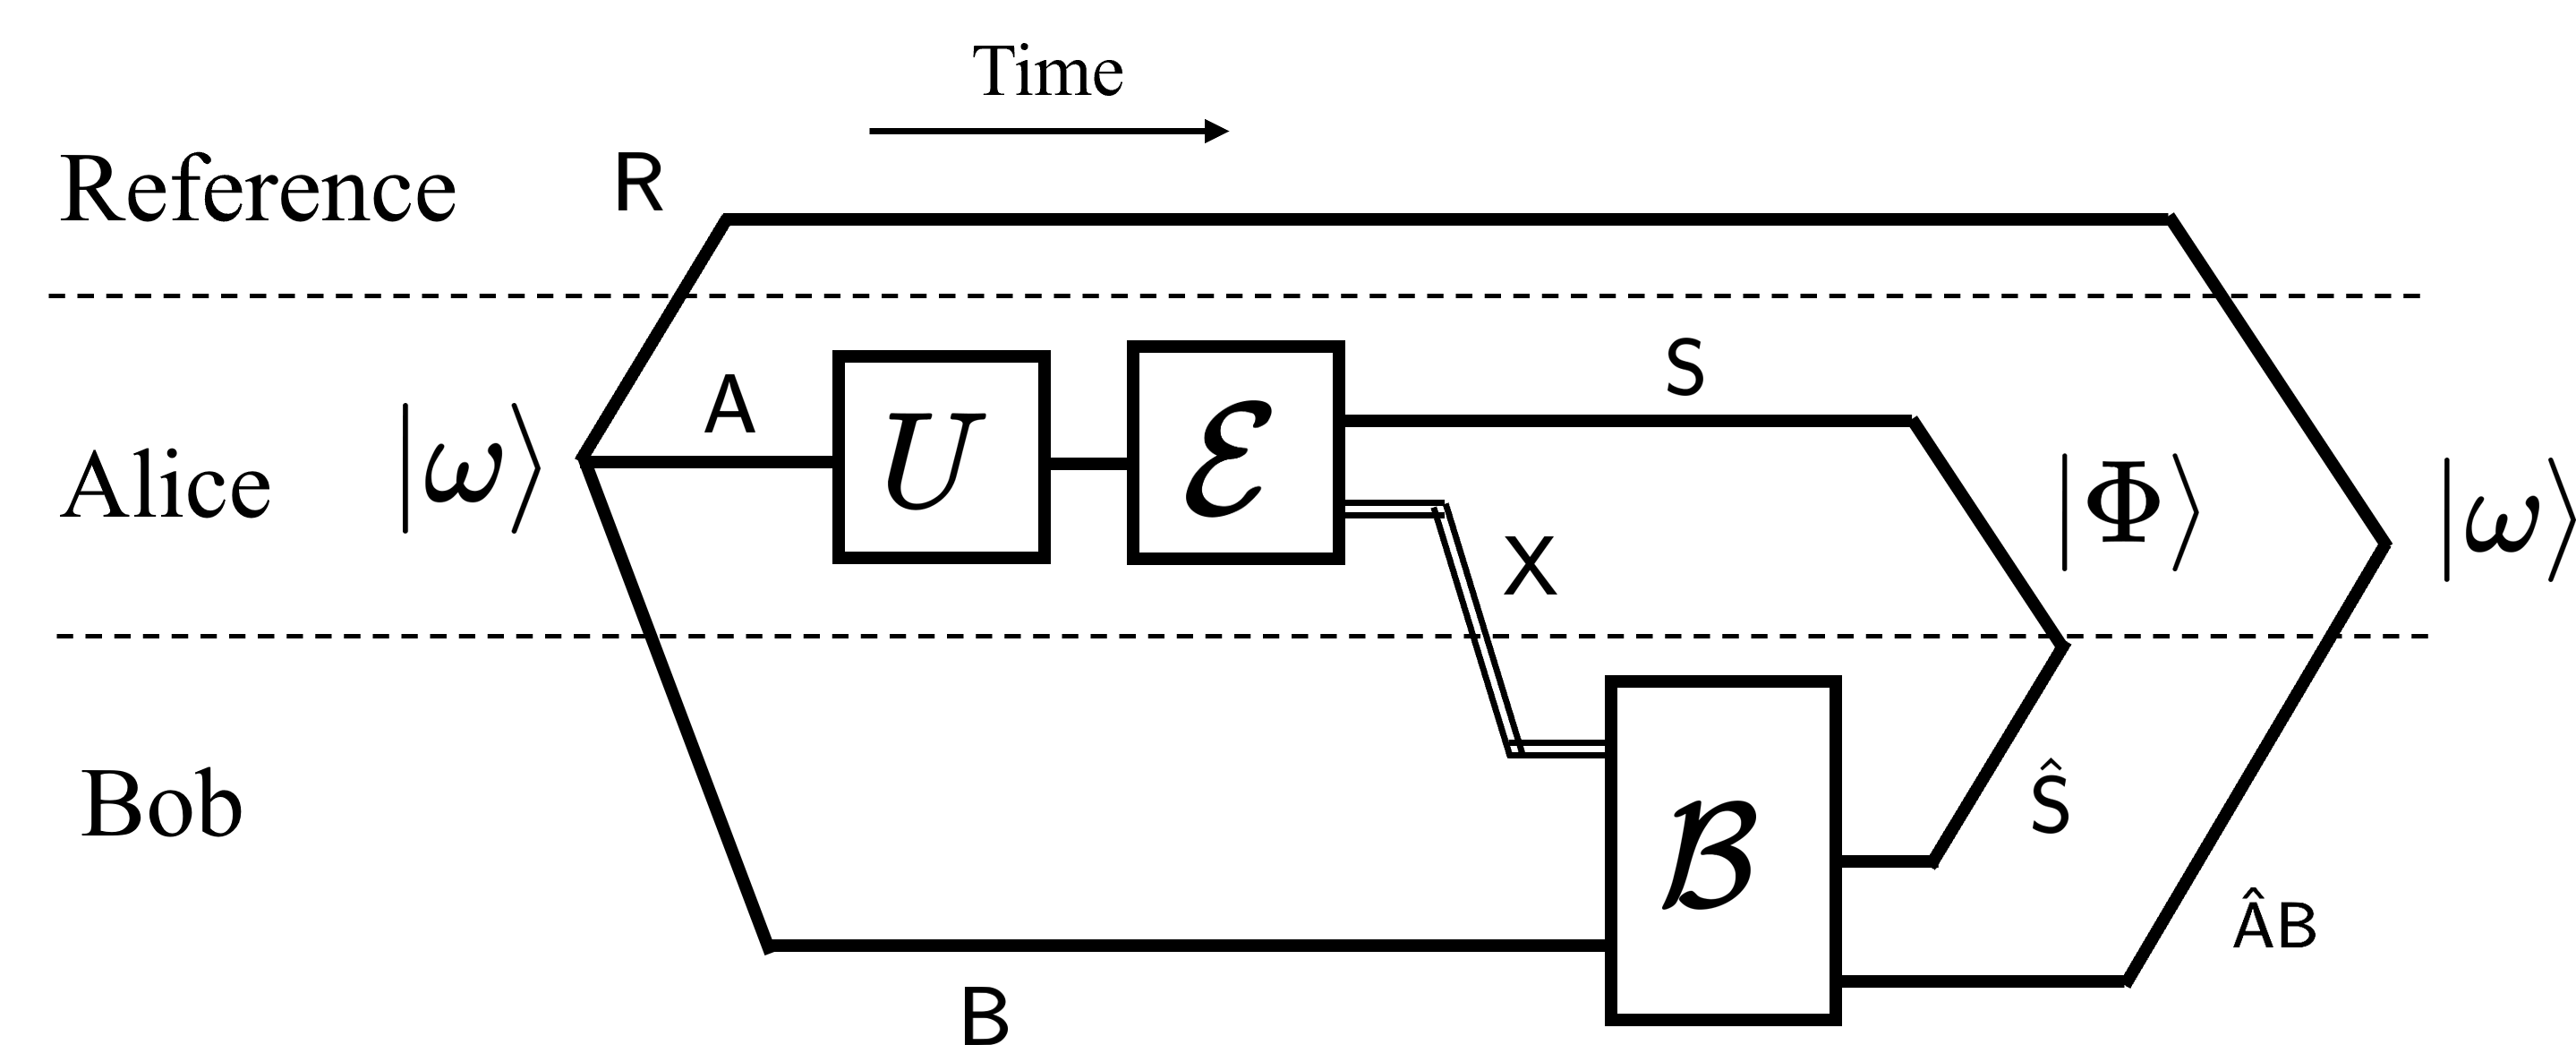
\includegraphics[width=100mm]{fig7.png}
    \caption{A diagram of quantum state merging.
    The goal is to transfer Alice's subsystem, which is part of a joint quantum state $\ket{\omega}^{\sR\sA\sB}$, to Bob, while simultaneously distilling as much entanglement as possible between $\sS$ and $\hat{\sS}$, using only local operations and classical communication.
    The double line connecting Alice and Bob represents a noiseless classical communication channel.
    }
    \label{fig:diagram of ent distill}
\end{figure}






After receiving the register $\sX$ by classical communication, which stores the measurement outcome $x$, Bob performs the operation $\cB^{\sB\sX \to \hat{\sA}\sB\hat{\sS}}$ specified as follows.
Let $\sqrt{p_x}\ket{\psi_x}^{\sR\sS\sB} = U_x^{\sA \to \sS} \Pi_x^\sA U^\sA\ket{\omega}^{\sR\sA\sB}$, where $p_x$ is the probability that the outcome $x$ occurs, and $\ket{\psi_x}^{\sR\sS\sB}$ is the resulting state.
Then, the operation $\cB^{\sB\sX \to \hat{\sA}\sB\hat{\sS}}$ is constructed as $\cB^{\sB\sX\rarr\hat{\sA}\sB\hat{\sS}} = \tr_\sX \circ \cW^{\hat{\sA}\sB\hat{\sS}\sX} \circ \cP_{\ket{0}}^{\bC\rarr\hat{\sA}\hat{\sS}}$, where $W^{\hat{\sA}\sB\hat{\sS}\sX}$ is a unitary such that $W^{\hat{\sA}\sB\hat{\sS}\sX} = \sum_x V_x^{\hat{\sA}\sB\hat{\sS}} \otimes \ketbra{x}{x}^\sX$, and $ V_x^{\hat{\sA}\sB\hat{\sS}}$ is the Uhlmann unitary satisfying 
\begin{align}
\label{inteq:111}
    \rF\big(V_x^{\hat{\sA}\sB\hat{\sS}}\ket{\psi_x}^{\sR\sS\sB}\ket{0}^{\hat{\sA}\hat{\sS}}, \ket{\omega}^{\sR\hat{\sA}\sB}\ket{\Phi}^{\sS\hat{\sS}}\big) = \rF(\psi_x^{\sR\sS}, \omega^\sR\otimes\pi^\sS).
\end{align}


We remark on the performance of the above protocol.
Let $\bar{\cE}^{\sA\rarr\sS\sE}$ be a complementary channel of $\cE^{\sA\rarr\sX} = \tr_\sS\circ\cE^{\sA\rarr\sS\sX}$, where $\sE$ is an environment of the classical channel from Alice to Bob.
We assume $d_\sE = d_\sX$ without loss of generality.
The decoupling theorem~\cite{dupuis2014one} ensures that the Haar random unitary $U^\sA$ satisfies
\begin{align}
\label{eq:OneShotDecouplingExpectDistill}
    \rF\big(\bar{\cE}^{\sA\rarr\sS\sE}\circ\cU^\sA(\omega^{\sR\sA}), \omega^\sR \otimes \pi^\sS \otimes \pi^\sE \big) \geq 1 - \epsilon,
\end{align}
with high probability.
Here, $\epsilon$ can be taken sufficiently small, depending on the properties of the initial state $\ket{\omega}^{\sR\sA\sB}$ and the channel $\cE^{\sA\rarr\sS\sX}$, such as the dimension of the system $\sS$ and the amount of initial entanglement between the systems $\sA$ and $\sB$~\cite{dupuis2014one}.
In Eq.~\eqref{eq:OneShotDecouplingExpectDistill}, the reduced Choi--Jamio\l kowski state on $\sS\sE$ is given by $\bar{\cE}^{\sA\rarr\sS\sE}(\pi^\sA) = \pi^\sS \otimes \pi^\sE$.
This is because, according to the outcome $x$, each $U_x^{\sA\rarr\sS}$ maps from $\cH_x^\sA$ to $\cH^\sS$, which is spanned by a fixed basis, and thus, $U_x^{\sA\rarr \sS}\Pi_x^\sA(U_x^{\sA\rarr\sS})^\dag$ is independent of $x$ and equals $\bI^\sS$.
Then, under the decoupling condition Eq.~\eqref{eq:OneShotDecouplingExpectDistill}, it is known that the operation $\cB^{\sB\sX\rarr\hat{\sA}\sB\hat{\sS}}$ achieves the task of quantum state merging with fidelity at least $1-\epsilon$. For details, see, e.g., Ref.~\cite{khatri2024principlemodern}.



%========================================================================================================================================================================================================================================





\subsubsection{Algorithmic implementation of Bob's operation based on the Uhlmann transformation}
\label{sec:implement uhl in state merging}


We consider explicitly implementing the unitary $W^{\hat{\sA}\sB\hat{\sS}\sX} = \sum_x V_x^{\hat{\sA}\sB\hat{\sS}} \otimes \ketbra{x}{x}^\sX$, using our Uhlmann transformation algorithm.
In this case, the Uhlmann unitary $V_x^{\hat{\sA}\sB\hat{\sS}}$ is conditioned by $x$ and should be realized for all $x$.
For algorithmic construction, we assume that Bob has full knowledge of Alice's operation $\cA^{\sA\rarr\sS\sX} = \cE^{\sA\rarr\sS\sX}\circ\cU^\sA$ and is capable of implementing it. 
While $U^\sA$ is chosen uniformly at random by Alice, Bob can identify the unitary Alice chose, for instance, using shared randomness.

We address the following model: 
\begin{itemize}
    \item A model in which multiple independent and identical copies of the initial state, $\ket{\omega}^{\sR'\sA'\sB'}$, are available.
\end{itemize}
We then evaluate the number of samples of $\ket{\omega}^{\sR'\sA'\sB'}$ required for Bob's operation.
We should distinguish the systems used by Bob, e.g., $\sR'$ and $\sA'$, from those that already exist as the reference $\sR$ and Alice's systems $\sA$.
The state $\ket{\omega}^{\sR'\sA'\sB'}$ is sampled and used \emph{locally} by Bob.
It is noteworthy that, in this model, Bob does not need to know a complete description of the initial state $\ket{\omega}^{\sR\sA\sB}$; rather, Bob is provided with copies of the state, whose description remains unknown to Bob.




We define a state $\ket{\Psi}^{\sR\sS\sB\sX\sE} = V_\cA^{\sA\rarr\sS\sX\sE}\ket{\omega}^{\sR\sA\sB}$, where $V_\cA^{\sA\rarr\sS\sX\sE}$ is a Stinespring isometry of $\cA^{\sA\rarr\sS\sX} = \cE^{\sA\rarr\sS\sX}\circ \cU^\sA$. 
We introduce $m_{\rm min}$ and $r_{\rm max}$ as  
\begin{align}
    \label{inteq:142}
    m_{\rm min} = \min_x\Big[\f{p_x}{d_\sX}s_{\rm min}\Big(\sqrt{\psi_x^{\sR\sS}}\big(\sqrt{\omega^\sR}\otimes\sqrt{\pi^\sS}\big)\Big)\Big], \ \ \ \text{and} \ \ \ r_{\rm max} = \max_x\Big[r\Big(\sqrt{\psi_x^{\sR\sS}}\big(\sqrt{\omega^\sR}\otimes\sqrt{\pi^\sS}\big)\Big)\Big],
\end{align}
where $s_{\rm min}(\cdot)$ and $r(\cdot)$ are the minimum non-zero singular value and the rank of an input matrix, respectively.
The maximization and minimization are taken over all outcomes $x$.


Our statement is as follows. 

\begin{theorem}[Uhlmann transformation algorithm in quantum state merging]
\label{thm:Uhlmann state merging}
    In the setting of quantum state merging, suppose that for some $\epsilon \in [0, 1]$,  
    \begin{align}
    \label{inteq:141}
            \rF\big(\Psi^{\sR\sS\sE}, \omega^\sR \otimes \pi^\sS \otimes \pi^\sE \big) \geq 1 - \epsilon.
    \end{align}
    Then, for $\delta \in (0, 1)$, there exists a quantum algorithm that implements a quantum channel $\til{\cB}^{\sB\sX\rarr\hat{\sA}\sB\hat{\sS}}$, which satisfies
    \begin{align}
        \rF\big(\til{\cB}^{\sB\sX\rarr\hat{\sA}\sB\hat{\sS}}(\Psi^{\sR\sS\sB\sX}), \ket{\omega}^{\sR\hat{\sA}\sB}\ket{\Phi}^{\sS\hat{\sS}}\big) \geq 1 - \epsilon - \delta,
    \end{align}
    using $\zeta$ samples of $\ket{\omega}^{\sR'\sA'\sB'}$, where $\zeta = \cO\Big(\f{1}{\delta^2}\min\Big\{\f{1}{m_{\rm min}^2}, \f{r_{\rm max}^2}{\delta^4}\Big\}\Big(\log{\Big(\f{1}{\delta}\Big)}\Big)^2\Big)$, and $m_{\rm min}$ and $r_{\rm max}$ are given by Eqs.~\eqref{inteq:142}. The quantum circuit for the algorithm consists of $\cO\big(\zeta\log{(d_\sR d_\sA d_\sB)}\big)$ one- and two-qubit gates, and $\cO\big(\log{(d_\sR d_\sA d_\sB)}\big)$ qubits suffice at any one time.
\end{theorem}



This theorem states that when $\Psi^{\sR\sS\sX}$ is sufficiently decoupled as $\Psi^{\sR\sS\sX} \approx \omega^\sR \otimes \pi^\sS \otimes \pi^\sX$ by Alice's operation, then by taking small $\delta$ and applying $\til{\cB}^{\sB\sX\rarr\hat{\sA}\sB\hat{\sS}}$---which is explicitly constructed using our algorithm---Bob can accomplish the task of quantum state merging.




\begin{proof}[Proof of Theorem~\ref{thm:Uhlmann state merging}]
    


Let $\sL = \sR\sS$ and $\sM = \hat{\sA}\sB\hat{\sS}$. 
We define $\ket{\sigma}^{\sL\sM}$ and $\Psi^{\sL\sM\sX}$ by $\ket{\sigma}^{\sL\sM} = \ket{\omega}^{\sR\hat{\sA}\sB}\ket{\Phi}^{\sS\hat{\sS}}$ and 
\begin{align}
    \Psi^{\sL\sM\sX} 
    &= \cP_{\ket{0}}^{\bC\rarr\hat{\sA}\hat{\sS}} \circ \cE^{\sA\rarr\sS\sX}\circ\cU^\sA(\ketbra{\omega}{\omega}^{\sR\sA\sB}) \\
    &= \sum_x  p_x\ketbra{\psi_x}{\psi_x}^{\sR\sS\sB} \otimes \ketbra{x}{x}^{\sX} \otimes \ketbra{0}{0}^{\hat{\sA}\hat{\sS}} \\
    &= \sum_x  p_x\ketbra{\rho_x}{\rho_x}^{\sL\sM} \otimes \ketbra{x}{x}^{\sX},
\end{align}
where $\ket{\rho_x}^{\sL\sM} = \ket{\psi_x}^{\sR\sS\sB}\ket{0}^{\hat{\sA}\hat{\sS}}$.
We then consider 
\begin{align}
    \cJ^{\sM\sH\hat{\sL}\hat{\sM}\sX} 
    = \mathtt{UhlmannPurifiedSample}(\Psi^{\sL'\sM'\sX'}, \sigma^{\sL'\sM'}\otimes\pi^{\sX'}; \delta_1, \tF),
\end{align}
where $\hat{\sL}$ and $\hat{\sM}$ are auxiliary systems of the same number of qubits as $\sL$ and $\sM$, respectively. 
Here, the inputs to $\mathtt{UhlmannPurifiedSample}$ are mixed states. This aims to transform $\ket{\rho_x}^{\sL\sM}$ to $\ket{\sigma}^{\sL\sM}$ for all $x$ by acting on $\sM\sX$.
The procedure and performance analysis of this channel is a direct extension of the one in \Cref{alg:Uhl purif sample} and Theorem~\ref{thm:algorithm Uhlmann}.


The quantum channel $\cJ^{\sM\sH\hat{\sL}\hat{\sM}\sX}$ satisfies 
\begin{align}
\label{inteq:133}
    \f{1}{2}\big\|\cJ^{\sM\sH\hat{\sL}\hat{\sM}\sX} - \cU_1^{\sM\sH\hat{\sL}\hat{\sM}\sX}\big\|_\diamond \leq \delta_1/2,
\end{align}
where $U_1^{\sM\sH\hat{\sL}\hat{\sM}\sX}$ is a block-encoding unitary of $\sum_x \ketbra{\rho_x}{\sigma}^{\hat{\sL}\hat{\sM}} \otimes \til{V}_x^\sM \otimes \ketbra{x}{x}^\sX$, $\til{V}_x^\sM = P_\sgn^{(\rm SV)}\big(\sin^{(\rm SV)}(M_x^\sM)\big)$, and $M_x^\sM = \f{p_x}{d_\sX} \tr_\sL[\ket{\sigma}\bra{\rho_x}^{\sL\sM}]$. (See also Eq.~\eqref{inteq:16} with rescaling by $\delta_2 \gets \delta_1/(2u)$).


Let $m_{\rm min}$ and $r_{\rm max}$ be defined by 
\begin{align}
\label{inteq:118}
    m_{\rm min}
    &= \min_x \big[s_{\rm min}(M_x^\sM)\big] \\
    &= \min_x \Big[\sqrt{\f{p_x}{d_\sX}}s_{\rm min}\Big(\sqrt{\Psi^{\sR\sS\sX}}\big(\sqrt{\omega^\sR}\otimes\sqrt{\pi^\sS}\otimes\pi^\sX\big)\Big)\Big] \\
    &= \min_x\Big[\f{p_x}{d_\sX}s_{\rm min}\Big(\sqrt{\psi_x^{\sR\sS}}\big(\sqrt{\omega^\sR}\otimes\sqrt{\pi^\sS}\big)\Big)\Big],
\end{align}
where $\Psi^{\sR\sS\sX} = \cE^{\sA\rarr\sS\sX}\circ\cU^\sA(\omega^{\sR\sA})$, and
\begin{align}
\label{inteq:119}
    r_{\rm max} 
    &= \max_x\big[r(M_x^\sM)\big] \\
    &= \max_x\Big[r\Big(\sqrt{\psi_x^{\sR\sS}}\big(\sqrt{\omega^\sR}\otimes\sqrt{\pi^\sS}\big)\Big)\Big],
\end{align}
where $s_{\rm min}(\cdot)$ and $r(\cdot)$ denote the minimum non-zero singular value and the rank of an input matrix, respectively.
The maximization and minimization over $x$ are crucial to ensure that the algorithm covers all $x$.


From the discussion in \Cref{sec:uhlfidpurifsamp} (especially, from Eq.~\eqref{inteq:120} to Eq.~\eqref{inteq:51} with rescaling by $\delta_1 \gets \delta_1/8$), when we set $\beta = \cO(\max\{m_{\rm min}, \delta_1/r_{\rm max}\})$, it holds that, for all $x$, 
\begin{align}
\label{inteq:113}
    \big|\sqrt{\rF}(\til{V}_x^\sM\ket{\rho_x}^{\sL\sM}, \ket{\sigma}^{\sL\sM}) - \sqrt{\rF}(V_x^\sM\ket{\rho_x}^{\sL\sM}, \ket{\sigma}^{\sL\sM})\big| \leq \delta_1/4.
\end{align}
Note that the Uhlmann partial isometry $V_x^\sM$ that satisfies Eq.~\eqref{inteq:111} is given by $V_x^\sM = \sgn^{(\rm SV)}\big(\sin^{(\rm SV)}(M_x^\sM)\big)$.



Let Bob's operation $\til{\cB}^{\sB\sX\rarr\hat{\sA}\sB\hat{\sS}}$ be given by  
\begin{align}
    \til{\cB}^{\sB\sX\rarr\hat{\sA}\sB\hat{\sS}} = \tr_{\sH\hat{\sL}\hat{\sM}\sX}\circ\cJ^{\sM\sH\hat{\sL}\hat{\sM}\sX}\circ\cP_{\ket{\sigma}}^{\bC\rarr\hat{\sL}\hat{\sM}}\circ\cP_{\ket{0}}^{\bC\rarr\sH\hat{\sA}\hat{\sS}}.
\end{align}
We then evaluate the fidelity between the state obtained by applying Alice's and Bob's operations to the initial state $\ket{\omega}^{\sR\sA\sB}$ and the target state $\ket{\sigma}^{\sL\sM} = \ket{\omega}^{\sR\hat{\sA}\sB}\ket{\Phi}^{\sS\hat{\sS}}$.
To this end, we define the following states:
\begin{align}
    &\xi^{\sL\sM\sH\hat{\sL}\hat{\sM}\sX} = \cJ^{\sM\sH\hat{\sL}\hat{\sM}\sX}\circ\cP_{\ket{\sigma}}^{\bC\rarr\hat{\sL}\hat{\sM}}\circ\cP_{\ket{0}}^{\bC\rarr\sH} (\Psi^{\sL\sM\sX}), \\
    &\xi_1^{\sL\sM\sH\hat{\sL}\hat{\sM}\sX} = \cU_1^{\sM\sH\hat{\sL}\hat{\sM}\sX}\circ\cP_{\ket{\sigma}}^{\bC\rarr\hat{\sL}\hat{\sM}}\circ\cP_{\ket{0}}^{\bC\rarr\sH} (\Psi^{\sL\sM\sX}), \\
    &\xi_{\rm ideal}^{\sL\sM\sH\hat{\sL}\hat{\sM}\sX} = \cU_{\rm ideal}^{\sM\sH\hat{\sL}\hat{\sM}\sX}\circ\cP_{\ket{\sigma}}^{\bC\rarr\hat{\sL}\hat{\sM}}\circ\cP_{\ket{0}}^{\bC\rarr\sH} (\Psi^{\sL\sM\sX}),
\end{align}
where $U_{\rm ideal}^{\sM\sH\hat{\sL}\hat{\sM}\sX}$ is the exact block-encoding unitary of $\sum_x \ketbra{\rho_x}{\sigma}^{\hat{\sL}\hat{\sM}}\otimes V_x^\sM \otimes\ketbra{x}{x}^\sX$.
We further define a reference state by
\begin{align}
    \phi_{\rm ref}^{\sL\sM\sH\hat{\sL}\hat{\sM}\sX} = \sum_x \f{1}{d_\sX}\ketbra{\rho_x}{\rho_x}^{\hat{\sL}\hat{\sM}} \otimes \ketbra{\sigma}{\sigma}^{\sL\sM} \otimes \ketbra{x}{x}^\sX \otimes \ketbra{0}{0}^\sH.
\end{align}

Let $\sN = \sL\sM\sH\hat{\sL}\hat{\sM}\sX$.
We first see that
\begin{align}
    \big|\sqrt{\rF}\big(\xi_1^\sN, \phi_{\rm ref}^\sN\big) - \sqrt{\rF}\big(\xi_{\rm ideal}^\sN, \phi_{\rm ref}^\sN\big)\big| 
    &= \Big|\sum_x\sqrt{\f{p_x}{d_\sX}}\sqrt{\rF}(\til{V}_x^\sM\ket{\rho_x}^{\sL\sM}, \ket{\sigma}^{\sL\sM}) - \sum_x\sqrt{\f{p_x}{d_\sX}}\sqrt{\rF}(V_x^\sM\ket{\rho_x}^{\sL\sM}, \ket{\sigma}^{\sL\sM})\Big| \\
    &\leq \sum_x\sqrt{\f{p_x}{d_\sX}}\big|\sqrt{\rF}(\til{V}_x^\sM\ket{\rho_x}^{\sL\sM}, \ket{\sigma}^{\sL\sM}) - \sqrt{\rF}(V_x^\sM\ket{\rho_x}^{\sL\sM}, \ket{\sigma}^{\sL\sM})\big| \\
    &\leq \f{\delta_1}{4}\sum_x\sqrt{\f{p_x}{d_\sX}} \\
    \label{inteq:114}
    &\leq \f{\delta_1}{4},
\end{align}
where we used Eq.~\eqref{inteq:113} in the second inequality and $\sum_x\sqrt{\f{p_x}{d_\sX}} \leq \sqrt{\sum_x p_x} = 1$ in the lase inequality.

Next, we observe that
\begin{align}
    \big|\sqrt{\rF}\big(\xi^\sN, \phi_{\rm ref}^\sN\big) - \sqrt{\rF}\big(\xi_1^\sN, \phi_{\rm ref}^\sN\big)\big|
    &= \Big| \Big\|\sqrt{\xi^\sN}\sqrt{\phi_{\rm ref}^\sN}\Big\|_1 -  \Big\|\sqrt{\xi_1^\sN}\sqrt{\phi_{\rm ref}^\sN}\Big\|_1\Big| \\
    &\leq \Big\| \sqrt{\xi^\sN}\sqrt{\phi_{\rm ref}^\sN} - \sqrt{\xi_1^\sN}\sqrt{\phi_{\rm ref}^\sN} \Big\|_1 \\
    &\leq \Big\|\sqrt{\xi^\sN} - \sqrt{\xi_1^\sN}\Big\|_2 \Big\|\sqrt{\phi_{\rm ref}^\sN}\Big\|_2 \\
    &\leq \big\|\xi^\sN - \xi_1^\sN\big\|_1^{1/2} \\
    &\leq \big\|\cJ^\sN - \cU_1^\sN \big\|_\diamond^{1/2} \\
    \label{inteq:115}
    &\leq \sqrt{\delta_1},
\end{align}
where we used the H\"{o}lder's inequality in Eq.~~\eqref{eq:Holder ineq} in the second inequality, and Eq.~\eqref{inteq:133} in the last inequality. The third inequality follows from $\Big\|\sqrt{\phi_{\rm ref}^\sN}\Big\|_2 = 1$ and the Powers--St\o rmer inequality in Eq.~\eqref{eq:powers stormer ineq}.
From Eqs.~\eqref{inteq:114} and~\eqref{inteq:115}, we obtain that
\begin{align}
\label{inteq:116}
    \big|\sqrt{\rF}\big(\xi^\sN, \phi_{\rm ref}^\sN\big) - \sqrt{\rF}\big(\xi_{\rm ideal}^\sN, \phi_{\rm ref}^\sN\big)\big| \leq \delta_1/4 + \sqrt{\delta_1}.
\end{align}



Using the above results, we can bound the fidelity between the final state $\Psi_{\rm fin}^{\sR\hat{\sA}\sB\sS\hat{\sS}} = \til{\cB}^{\sB\sX\rarr\hat{\sA}\sB\hat{\sS}}\circ\cA^{\sA\rarr\sS\sX}(\omega^{\sR\sA\sB})$ and the target state $\ket{\omega}^{\sR\hat{\sA}\sB}\ket{\Phi}^{\sS\hat{\sS}}$ as
\begin{align}
    \sqrt{\rF}\big(\Psi_{\rm fin}^{\sR\hat{\sA}\sB\sS\hat{\sS}}, \ket{\omega}^{\sR\hat{\sA}\sB}\ket{\Phi}^{\sS\hat{\sS}}) 
    &\geq \sqrt{\rF}\big(\xi^\sN, \phi_{\rm ref}^{\sN}\big) \\
    &\geq \sqrt{\rF}\big(\xi_{\rm ideal}^\sN, \phi_{\rm ref}^\sN\big) - \delta_1/4 - \sqrt{\delta_1} \\
    &= \sum_x \sqrt{\f{p_x}{d_\sX}}\sqrt{\rF}\big(V_x^\sM\ket{\rho_x}^{\sL\sM}, \ket{\sigma}^{\sL\sM}\big) - \delta_1/4 - \sqrt{\delta_1} \\
    &= \sum_x \sqrt{\f{p_x}{d_\sX}}\sqrt{\rF}(\psi_x^{\sR\sS}, \omega^\sR \otimes \pi^\sS) - \delta_1/4 - \sqrt{\delta_1} \\
    &= \sqrt{\rF}(\Psi^{\sR\sS\sE}, \omega^\sR \otimes \pi^\sS \otimes \pi^\sE) - \delta_1/4 - \sqrt{\delta_1},
\end{align}
where we used the fact that $\tr_{\sH\hat{\sL}\hat{\sM}\sX}[\xi^\sN] = \Psi_{\rm fin}^{\sR\hat{\sA}\sB\sS\hat{\sS}}$ and $\tr_{\sH\hat{\sL}\hat{\sM}\sX}[\phi_{\rm ref}^\sN] = \sigma^{\sL\sM} = \omega^{\sR\hat{\sA}\sB}\otimes\Phi^{\sS\hat{\sS}}$ in the first inequality.
We further applied Eq.~\eqref{inteq:116} in the second inequality and Eq.~\eqref{inteq:111} in the second equation.
Thus, noting that fidelity is always less than or equal to one, we have
\begin{align}
    \rF\big(\Psi_{\rm fin}^{\sR\hat{\sA}\sB\sS\hat{\sS}}, \ket{\omega}^{\sR\hat{\sA}\sB} \ket{\Phi}^{\sS\hat{\sS}}\big)
    &\geq \rF(\Psi^{\sR\sS\sE}, \omega^\sR \otimes \pi^\sS \otimes \pi^\sE) - 2(\delta_1/4 + \sqrt{\delta_1}) \\
    \label{inteq:112}
    &\geq 1 - \epsilon - 2(\delta_1/4 + \sqrt{\delta_1}),
\end{align}
where the last inequality follows from the condition Eq.~\eqref{inteq:141}.
Rescaling $\delta_1$ as $\delta_1 = (2\delta/5)^2$, we have $2(\delta_1/4 + \sqrt{\delta_1}) \leq \delta$.
Hence, since $\Psi_{\rm fin}^{\sR\hat{\sA}\sB\sS\hat{\sS}} = \til{\cB}^{\sB\sX\rarr\hat{\sA}\sB\hat{\sS}}\circ\cA^{\sA\rarr\sS\sX}(\omega^{\sR\sA\sB})$, we finally obtain 
\begin{align}
    \rF\big(\til{\cB}^{\sB\sX\rarr\hat{\sA}\sB\hat{\sS}}\circ\cA^{\sA\rarr\sS\sX}(\omega^{\sR\sA\sB}), \ket{\omega}^{\sR\hat{\sA}\sB} \ket{\Phi}^{\sS\hat{\sS}}\big) \geq 1 - \epsilon - \delta.
\end{align}



From Theorem~\ref{thm:algorithm Uhlmann}, the number of samples of $\Psi^{\sL'\sM'\sX'}$ and $\sigma^{\sL'\sM'}\otimes\pi^{\sX'}$ for implementing 
\begin{align}
    \mathtt{UhlmannPurifSample}(\Psi^{\sL'\sM'\sX'}, \sigma^{\sL'\sM'}\otimes\pi^{\sX'}; \delta_1, \tF) 
\end{align}
is given by $\cO\Big(\big(\log{(1/\delta_1)}\big)^2/(\delta_1\beta^2)\Big)$. 
Both $\Psi^{\sL'\sM'\sX'}$ and $\sigma^{\sL'\sM'}$ are prepared from a single copy of $\ket{\omega}^{\sR'\sA'\sB'}$. 
Recalling that $\beta = \cO(\max\{m_{\rm min}, \delta_1/r_{\rm max}\})$ and $\delta_1 \leq (2\delta/5)^2$, we evaluate the number of samples of $\ket{\omega}^{\sR'\sA'\sB'}$ for Bob's operation $\til{\cB}^{\sB\sX \rarr\hat{\sA}\sB\hat{\sS}}$ as
\begin{align}
    \zeta 
    &= \cO\Big(\f{1}{\delta_1\beta^2}\Big(\log{\Big(\f{1}{\delta_1}\Big)}\Big)^2\Big) \notag\\
    &= \cO\Big(\f{1}{\delta^2}\min\Big\{\f{1}{m_{\rm min}^2}, \f{r_{\rm max}^2}{\delta^4}\Big\}\Big(\log{\Big(\f{1}{\delta}\Big)}\Big)^2\Big),
\end{align}
where $m_{\rm min}$ and $r_{\rm max}$ are given by Eqs.~\eqref{inteq:118} and~\eqref{inteq:119}, respectively.
The quantum circuit of overall this algorithm includes $\cO\big(\zeta\log{(d_\sR d_\sA d_\sB)}\big)$ one- and two-qubit gates, and $\cO\big(\log{(d_\sR d_\sA d_\sB)}\big)$ qubits at any one time.




\end{proof}















%===============================================================================================================================================












\section{Application 3: Petz recovery map with the Uhlmann transformation algorithm}
\label{sec:sample petz}





The Petz recovery map~\cite{petz1986sufficient, petz1988sufficiency} is a powerful tool with broad applications in quantum science~\cite{barnum2002reversing, ng2010simpleapproach, beigi2016decoding, chen2020entanglement, lauten2022approx, nakayama2023petz}.
In particular, it is known that the map demonstrates nearly optimal performance when it reverses the effect of noise~\cite{barnum2002reversing, beigi2016decoding}.
The Petz recovery map $\cR_{\sigma, \cF}^{\sB \rarr \sA}$ is defined for a reference state $\sigma^\sA$ and a quantum channel $\cF^{\sA\rarr\sB}$ as $\cR_{\sigma, \cF}^{\sB \rarr \sA} = \cQ_{\sigma^{1/2}}^\sA\circ(\cF^{\sA\rarr\sB})^\dag\circ\cQ_{\cF(\sigma)^{-1/2}}^\sB$, where $(\cF^{\sA\rarr\sB})^\dag$ is an adjoint map of $\cF^{\sA\rarr\sB}$ and $\cQ_{\mu}^\sC = \mu^\sC(\cdot)\mu^\sC$ for an operator $\mu^\sC$.
The adjoint map $(\cF^{\sA\rarr\sB})^\dag$ of $\cF^{\sA\rarr\sB}$ is defined as the map satisfying $\tr[L^\sB\cF^{\sA\rarr\sB}(M^\sA)]=\tr[(\cF^{\sA\rarr\sB})^\dag(L^\sB)M^\sA]$ for any operators $L^\sB$ and $M^\sA$.


Quantum algorithms for the Petz recovery map have been studied in Refs.~\cite{gilyen2022petzmap, biswas2023noiseadapted}.
These works represent significant progress toward implementation of the map, but their approaches require, in addition to the use of $\sigma^\sA$, access to a Stinespring unitary of the channel $\cF^{\sA\rarr\sB}$ and its inverse, which is challenging in practice.


We here introduce a method to realize the Petz recovery map using only $\sigma^{\sA}$ and $\cF^{\sA\rarr\sB}$; that is, access to a Stinespring unitary is not required.
The implementation of $(\sigma^{\sA})^{1/2}$ and $\big(\cF^{\sA \rarr \sB}(\sigma^\sA)\big)^{-1/2}$ via block-encodings, directly using the density matrix exponentiation and the QSVT with multiple uses of $\sigma^{\sA}$ and $\cF^{\sA \rarr \sB}$, is straightforward (see, e.g., Refs.~\cite{gilyen2022petzmap, gilyen2022improvedfidelity, wang2023SampletoQuary, wang2024TimeEfficientEntEstSamp} for references).
Hence, we focus our investigation only on the non-trivial part $(\cF^{\sA\rarr\sB})^\dag$.
To this end, we make use of the following proposition, in which $(\cP_{\ket{0}}^{\bC\rarr\sG})^\dag$ denotes a linear map (not a quantum channel), defined as $(\cP_{\ket{0}}^{\bC\rarr\sG})^\dag(\cdot) = \bra{0}^\sG \cdot \ket{0}^\sG$.





\begin{proposition}[Implementation of a Stinespring unitary via the Uhlmann transformation algorithm]
\label{prop:stinespring unitary via uhlmann}
Let $\delta \in (0, 1)$. For any quantum channel $\cF^{\sA\rarr\sB}$, there exists a quantum algorithm that implements a quantum channel $\cG^\sS$ satisfying 
\begin{align}
    \f{1}{2}\big\|\cG^\sS \circ \cP_{\ket{0}}^{\bC\rarr\sG} - \cU_\cF^\sS \circ \cP_{\ket{0}}^{\bC\rarr\sG}\big\|_\diamond \leq \delta, 
\end{align}
where $\cU_\cF^\sS$ is a Stinespring unitary of $\cF^{\sA\rarr\sB}$ on $\sS = \sA\sG = \sB\sE$, with the dimension of $\sE$ taken as $d_\sE = d_\sA d_\sB$.
The algorithm uses the channel $\cF^{\sA \rarr \sB}$ a total of $\nu$ times, where $\nu = \til{\cO}\Big(\f{d_\sA^4 d_\sB}{\delta^2}\min\Big\{\f{1}{\tau_{\rm min}^2}, \f{d_\sA^6d_\sB^2}{\delta^4}\Big\}\Big)$, and $\tau_{\rm min}$ is the minimum non-zero eigenvalue of the Choi--Jamio\l kowski state $\tau^{\sR\sB} = \cF^{\sA\rarr\sB}(\Phi^{\sR\sA})$.

Moreover, there exists a quantum algorithm that implements a quantum channel $\cG_{\rm inv}^\sS$ satisfying 
\begin{align}
    \f{1}{2}\big\|(\cP_{\ket{0}}^{\bC\rarr\sG})^\dag\circ\cG_{\rm inv}^\sS - (\cP_{\ket{0}}^{\bC\rarr\sG})^\dag\circ(\cU_\cF^\sS)^\dag\big\|_\diamond \leq \delta,
\end{align}
also using $\cF^{\sA\rarr\sB}$ a total of $\nu$ times.

In both algorithms, $\cO\big(\log{(d_\sA d_\sB)}\big)$ qubits suffice at any one time.

\end{proposition}


Proposition~\ref{prop:stinespring unitary via uhlmann} will be proven at the end of this section.





For an algorithmic implementation of the Petz recovery map, we follow the protocol in Ref.~\cite{gilyen2022petzmap}.
The Petz recovery map can be rephrased as
\begin{align}
\label{eq:petz exp form rephrase}
    \cR_{\sigma, \cF}^{\sB \rarr \sA}
    &= d_\sE\cQ_{\sigma^{1/2}}^\sA\circ(\cP_{\ket{0}}^{\bC\rarr\sG})^\dag \circ(\cU_\cF^{\sS})^\dag \circ\cP_\pi^{\bC\rarr\sE}\circ\cQ_{\cF(\sigma)^{-1/2}}^\sB,
\end{align}
where $\sS = \sA\sG = \sB\sE$.
Since the size of the system $\sE$ is arbitrarily chosen, we set $\sE = \sR'\sB'$ with dimension $d_\sE = d_\sA d_\sB$. Note that $d_\sR = d_\sA$.
While post-selection by $\ket{0}^\sG$ may seem necessary, it can in fact be removed using the robust oblivious amplitude amplification~\cite{gilyen2019qsvt, Gilyn2019thesis} by iteratively applying $U_\cF^\sS$ and $(U_\cF^\sS)^\dag$ a total of $v = \cO\big(\sqrt{d_\sA d_\sB/\lambda_{\rm min}}\big)$ times~\cite{gilyen2022petzmap}.
Here, $\lambda_{\rm min}$ denotes the minimum non-zero eigenvalue of $\cF^{\sA\rarr\sB}(\sigma^\sA)$.
Hence, an approximate Petz recovery map can be deterministically implemented.




In the $v$ repetitions of $U_\cF^\sS$ and $(U_\cF^\sS)^\dag$ in the oblivious amplitude amplification, when we approximate these unitaries by $\cG^\sS$ and $\cG_{\rm inv}^\sS$ within an error $\delta$, respectively, the total error accumulates to $v\delta$.
By rescaling $\delta$ as $\delta = \epsilon/v$, we implement the approximation of the Petz recovery map with error at most $\epsilon$ in the diamond norm, using $\cF^{\sA \rarr \sB}$ the following total number of times:
\begin{align}
\label{eq:sampcomp Petz}
    v\til{\cO}\Big(\f{d_\sA^4 d_\sB}{(\epsilon/v)^2 }\min\Big\{\f{1}{\tau_{\rm min}^2}, \f{d_\sA^6d_\sB^2}{(\epsilon/v)^4}\Big\}\Big) =\til{\cO}\Big(\f{d_\sA^{11/2} d_\sB^{5/2}}{\epsilon^2  \lambda_{\rm min}^{3/2}}\min\Big\{\f{1}{\tau_{\rm min}^2}, \f{d_\sA^8 d_\sB^4}{\epsilon^4\lambda_{\rm min}^2}\Big\}\Big).
\end{align}


To be precise, implementing $\cQ_{\sigma^{1/2}}^\sA$ and $\cQ_{\cF(\sigma)^{-1/2}}^\sB$ additionally requires access to $\sigma^\sA$ and $\cF^{\sA\rarr\sB}$.
However, as mentioned, since these can be straightforwardly realized using the density matrix exponentiation and the QSVT, we do not provide a detailed discussion here.







Other approaches to implementing the Petz recovery map $\cR_{\sigma, \cF}^{\sB\rarr\sA}$ using only the channel $\cF^{\sA\rarr\sB}$ and the state $\sigma^\sA$ may be possible. 
In fact, since the map is independent of the choice of the system $\sE$ (see Eq.~\eqref{eq:petz exp form rephrase}), the recent results in Ref.~\cite{tang2025conjugatequerieshelp} based on the random purification techniques appear to be applicable. 
This approach would achieve computational costs of roughly the square of those in Ref.~\cite{gilyen2022petzmap} divided by the accuracy, although it would require collective measurements over an exponential number of Choi--Jamio\l kowski states of $\cF^{\sA\rarr\sB}$.
We leave a detailed investigation of this approach for future work.







We now prove \Cref{prop:stinespring unitary via uhlmann}.


\begin{proof}[Proof of \Cref{prop:stinespring unitary via uhlmann}]
    


We consider a purified state of the Choi--Jamio\l kowski state $\tau^{\sR\sB} = \cF^{\sA\rarr\sB}(\Phi^{\sR\sA})$, which is given by $\ket{\tau}^{\sR\sB\sE} = U_\cF^{\sS}\ket{\Phi}^{\sR\sA}\ket{0}^{\sG}$, where $U_\cF^{\sS}$ is a Stinespring unitary of $\cF^{\sA\rarr\sB}$ and $\sS = \sA\sG = \sB\sE$. Without loss of generality, we take $d_\sR = d_\sA$. 
Since $\tau^{\sR} = \pi^{\sR}$, we observe that $U_\cF^\sS$ corresponds to the Uhlmann unitary transforming $\ket{\Phi}^{\sR\sA}\ket{0}^{\sG}$ to $\ket{\tau}^{\sR\sB\sE}$.
Thus, using our Uhlmann transformation algorithm for $\ket{\Phi}^{\sR\sA}\ket{0}^{\sG}$ and $\ket{\tau}^{\sR\sB\sE}$, the unitary $U_\cF^{\sS}$ can be implemented.


To generate a purified state of $\tau^{\sR\sB}$, we use the canonical purification: $\ket{\tau_{\rm c}}^{\sR\sB\sR'\sB'} = (\sqrt{\tau^{\sR\sB}} \otimes \bI^{\sR'\sB'})\ket{\Gamma}^{\sR\sB\sR'\sB'}$. Note that the environment $\sE$ is chosen to be $\sR'\sB'$ in the canonical purification. 
Thus, $\sS = \sA\sG = \sB\sR'\sB'$.
From \Cref{prop:canonical purification}, to obtain a state $\til{\tau}_{\rm c}^{\sR\sS} = \mathtt{CanonicalPurification}(\tau^{\sR\sB}; \delta_1)$ that approximates $\ket{\tau_{\rm c}}^{\sR\sS}$ with the error $\delta_1$ in the trace distance: $\f{1}{2}\big\|\til{\tau}_{\rm c}^{\sR\sS} - \ketbra{\tau_{\rm c}}{\tau_{\rm c}}^{\sR\sS}\big\|_1 \leq \delta_1$, we use $f$ samples of $\tau^{\sR\sB}$, where $f = \til{\cO}\Big(\f{d_\sA d_\sB}{\delta_1}\min\Big\{ \f{1}{\tau_{\rm min}^2}, \f{d_\sA^2 d_\sB^2}{\delta_1^4}\Big\}\Big)$, and $\tau_{\rm min}$ is the non- zero minimum eigenvalue of $\tau^{\sR\sB}$.



Next, we apply the Uhlmann transformation algorithm with $\ket{\sigma}^{\sR\sS} = \ket{\Phi}^{\sR\sA}\ket{0}^{\sG}$ and $\til{\tau}_{\rm c}^{\sR\sS}$ to obtain an approximation of the unitary $U_\cF^\sS$.
At this point, a careful analysis is needed, since the Uhlmann transformation algorithm realizes a partial isometry $W_\cF^\sS$, not the full unitary $U_\cF^\sS$.
However, this does not cause any critical issue, as we will show below.



The relation between the partial isometry $W_\cF^\sS$ and the Stinespring unitary $U_\cF^\sS$ is that $W_\cF^\sS$ is embedded in the part of $U_\cF^\sS$ specified by projections $\ketbra{0}{0}^\sG\otimes\bI^\sA$ and $\Pi_\cF^{\sB\sR'\sB'} = V_\cF^{\sA\rarr\sB\sR'\sB'}(V_\cF^{\sA\rarr\sB\sR'\sB'})^\dag$, where $V_\cF^{\sA\rarr\sB\sR'\sB'}$ is a Stinespring isometry of $\cF$. That is, 
\begin{align}
        U_\cF^\sS
        = \hspace{1mm}
\begin{blockarray}{ccc}
 & \ketbra{0}{0}^\sG\otimes\bI^\sA &  & \vspace{1mm}\\
\begin{block}{c(cc)}
  \Pi_\cF^{\sB\sR'\sB'} \hspace*{1mm} & W_\cF^\sS & \hspace{0mm} * \hspace{3mm}\\
   \hspace*{1mm} & * & \hspace{0mm} * \hspace{3mm}\\
\end{block}
\end{blockarray}\hspace{2.5mm}.
\end{align}
Then, the following relation holds:
\begin{align}
    U_\cF^\sS\ket{0}^\sG 
    &= V_\cF^{\sA\rarr\sB\sR'\sB'} \\
    &= V_\cF^{\sA\rarr\sB\sR'\sB'}(V_\cF^{\sA\rarr\sB\sR'\sB'})^\dag V_\cF^{\sA\rarr\sB\sR'\sB'} \\
    &= \Pi_\cF^{\sB\sR'\sB'} U_\cF^{\sS} (\ketbra{0}{0}^\sG\otimes\bI^\sA) \ket{0}^\sG \\
    & = W_\cF^\sS \ket{0}^\sG.
\end{align}
Hence, when we fix an input on the system $\sG$ as $\ket{0}^\sG$, the actions of them are identical.


Let $U_{\rm ideal}^{\sS\sH\hat{\sR}\hat{\sS}}$ be an exact block-encoding unitary of $\ketbra{\sigma}{\tau_{\rm c}}^{\hat{\sR}\hat{\sS}} \otimes W_\cF^\sS$.
Then, a quantum channel $\cJ^{\sS\sH\hat{\sR}\hat{\sS}} = \mathtt{UhlmannPurifiedSample}(\ket{\sigma}^{\sR\sS}, \til{\tau}_{\rm c}^{\sR\sS}; \delta_2, \diamond)$ satisfies
\begin{align}
\label{inteq:122}
    \f{1}{2}\big\|\cJ^{\sS\sH\hat{\sR}\hat{\sS}}\circ\cP_{\ket{0}}^{\bC\rarr\sH}\circ\cP_{\til{\tau}_{\rm c}}^{\bC\rarr\hat{\sR}\hat{\sS}} - \cU_{\rm ideal}^{\sS\sH\hat{\sR}\hat{\sS}} \circ \cP_{\ket{0}\ket{\tau_{\rm c}}}^{\bC\rarr\sH\hat{\sR}\hat{\sS}}\big\|_\diamond \leq \delta_2 + (2u+1)\delta_1,
\end{align}
where $u=\cO\big(d_\sA\log{(1/\delta_2)}\big)$.
The number of samples of $\til{\tau}_{\rm c}^{\sR\sB\sR'\sB'}$ and $\ket{\sigma}^{\sR\sS}$ is given by 
\begin{align}
    w =\cO\big(d_\sA^2\big(\log{(1/\delta_2)}\big)^2/\delta_2\big).
\end{align}
We here used the fact that the minimum non-zero singular value of $\sqrt{\pi^{\sR}}\sqrt{\tau_{\rm c}^{\sR}} = \pi^\sR$ is $1/d_\sA$.
The case where one input to $\mathtt{UhlmannPurifiedSample}$ is a mixed state $\til{\tau}_{\rm c}^{\sR\sS}$ can be handled by a similar argument to that in \Cref{sec:proof eval sample mixed}.

Note that $U_{\rm ideal}^{\sS\sH\hat{\sR}\hat{\sS}}\ket{0}^{\sH}\ket{\tau_{\rm c}}^{\hat{\sR}\hat{\sS}}\ket{0}^\sG = \ket{0}^\sH\ket{\sigma}^{\hat{\sR}\hat{\sS}}W_\cF^\sS\ket{0}^\sG = \ket{0}^\sH\ket{\sigma}^{\hat{\sR}\hat{\sS}}U_\cF^\sS\ket{0}^\sG$.
When we define a quantum channel $\cG^\sS$ as $\cG^\sS = \tr_{\sH\hat{\sR}\hat{\sS}} \circ \cJ^{\sS\sH\hat{\sR}\hat{\sS}} \circ \cP_{\ket{0}}^{\bC\rarr\sH}\circ\cP_{\til{\tau}_{\rm c}}^{\bC\rarr\hat{\sR}\hat{\sS}}$, we have that
\begin{align}
    &\f{1}{2}\big\|\cG^\sS\circ\cP_{\ket{0}}^{\bC\rarr\sG} - \cU_\cF^\sS\circ\cP_{\ket{0}}^{\bC\rarr\sG}\big\|_\diamond \notag \\
    &\leq \f{1}{2}\big\|\cJ^{\sS\sH\hat{\sR}\hat{\sS}}\circ\cP_{\ket{0}}^{\bC\rarr\sH}\circ\cP_{\til{\tau}_{\rm c}}^{\bC\rarr\hat{\sR}\hat{\sS}}\circ\cP_{\ket{0}}^{\bC\rarr\sG} - \cU_{\rm ideal}^{\sS\sH\hat{\sR}\hat{\sS}}\circ\cP_{\ket{0}}^{\bC\rarr\sH}\circ\cP_{\ket{\tau_{\rm c}}}^{\bC\rarr\hat{\sR}\hat{\sS}}\circ\cP_{\ket{0}}^{\bC\rarr\sG}\big\|_\diamond \\
    &\leq \f{1}{2}\big\|\cJ^{\sS\sH\hat{\sR}\hat{\sS}}\circ\cP_{\ket{0}}^{\bC\rarr\sH}\circ\cP_{\til{\tau}_{\rm c}}^{\bC\rarr\hat{\sR}\hat{\sS}} - \cU_{\rm ideal}^{\sS\sH\hat{\sR}\hat{\sS}} \circ \cP_{\ket{0}\ket{\tau_{\rm c}}}^{\bC\rarr\sH\hat{\sR}\hat{\sS}}\big\|_\diamond \\
    &\leq \delta_2 + (2u+1)\delta_1,
\end{align}
where we used Eq.~\eqref{inteq:122} in the third inequality.
Rescaling $\delta_1$ and $\delta_2$ as $\delta_1 = \delta/\big(2(2u+1)\big)$ and $\delta_2 = \delta/2$, the over all error is bounded from above by $\delta$.

In this algorithm, the number of uses of the quantum channel $\cF^{\sA\rarr\sB}$ is evaluated as
\begin{align}
    \nu 
    &= fw \\
    \label{inteq:19}
    &= \til{\cO}\Big(\f{d_\sA^4 d_\sB}{\delta^2}\min\Big\{\f{1}{\tau_{\rm min}^2}, \f{d_\sA^6d_\sB^2}{\delta^4}\Big\}\Big).
\end{align}


Constructing a quantum algorithm for approximating $(U_\cF^\sS)^\dag$ can be achieved straightforwardly using the fact that the Uhlmann unitary from $\ket{\tau_{\rm c}}^{\sR\sS}$ to $\ket{\sigma}^{\sR\sS} = \ket{\Phi}^{\sR\sA}\ket{0}^\sG$ coincides with $(U_\cF^\sS)^\dag$.
Hence, a quantum channel $\cJ_{\rm inv}^{\sS\sH\hat{\sR}\hat{\sS}} = \mathtt{UhlmannPurifiedSample}(\til{\tau}_{\rm c}^{\sR\sS}, \ket{\sigma}^{\sR\sS}; \delta_2, \diamond)$ satisfies that
\begin{align}
\label{inteq:123}
    &\f{1}{2}\big\|\cJ_{\rm inv}^{\sS\sH\hat{\sR}\hat{\sS}}\circ\cP_{\ket{0}\ket{\sigma}}^{\bC\rarr\sH\hat{\sR}\hat{\sS}} - (\cU_{\rm ideal}^{\sS\sH\hat{\sR}\hat{\sS}})^\dag \circ \cP_{\ket{0}\ket{\sigma}}^{\bC\rarr\sH\hat{\sR}\hat{\sS}}\big\|_\diamond 
    \leq \delta_2 + 2u\delta_1.
\end{align}
Note that, compared to the previous case for $U_\cF^\sS$, the first and second arguments of $\mathtt{UhlmannPurifiedSample}$ are swapped.


We observe that  $\bra{0}^\sG(U_{\rm ideal}^{\sS\sH\hat{\sR}\hat{\sS}})^\dag\ket{0}^{\sH}\ket{\sigma}^{\hat{\sR}\hat{\sS}} = \ket{0}^\sH\ket{\tau_{\rm c}}^{\hat{\sR}\hat{\sS}}\bra{0}^\sG(W_\cF^\sS)^\dag = \ket{0}^\sH\ket{\tau_{\rm c}}^{\hat{\sR}\hat{\sS}}\bra{0}^\sG (U_\cF^\sS)^\dag$.
Defining a quantum channel $\cG_{\rm inv}^\sS$ as $\cG_{\rm inv}^\sS = \tr_{\sH\hat{\sR}\hat{\sS}} \circ \cJ_{\rm inv}^{\sS\sH\hat{\sR}\hat{\sS}} \circ \cP_{\ket{0}\ket{\sigma}}^{\bC\rarr\sH\hat{\sR}\hat{\sS}}$, we see that it satisfies
\begin{align}
    &\f{1}{2}\big\|(\cP_{\ket{0}}^{\cC\rarr\sG})^\dag\circ\cG_{\rm inv}^\sS
    - (\cP_{\ket{0}}^{\cC\rarr\sG})^\dag\circ(\cU_\cF^\sS)^\dag\big\|_\diamond \\
    &\leq \f{1}{2}\big\|(\cP_{\ket{0}}^{\cC\rarr\sG})^\dag\circ \cJ_{\rm inv}^{\sS\sH\hat{\sR}\hat{\sS}}\circ\cP_{\ket{0}\ket{\sigma}}^{\bC\rarr\sH\hat{\sR}\hat{\sS}} - (\cP_{\ket{0}}^{\cC\rarr\sG})^\dag\circ(\cU_{\rm ideal}^{\sS\sH\hat{\sR}\hat{\sS}})^\dag\circ\cP_{\ket{0}\ket{\sigma}}^{\bC\rarr\sH\hat{\sR}\hat{\sS}}\big\|_\diamond \\
    &\leq \f{1}{2}\big\|(\cP_{\ket{0}}^{\cC\rarr\sG})^\dag\|_\diamond \big\|\cJ_{\rm inv}^{\sS\sH\hat{\sR}\hat{\sS}}\circ\cP_{\ket{0}\ket{\sigma}}^{\bC\rarr\sH\hat{\sR}\hat{\sS}} - (\cU_{\rm ideal}^{\sS\sH\hat{\sR}\hat{\sS}})^\dag\circ\cP_{\ket{0}\ket{\sigma}}^{\bC\rarr\sH\hat{\sR}\hat{\sS}}\big\|_\diamond \\
    &\leq \delta_2 + 2u\delta_1,
\end{align}
where in the second inequality, we used the fact that, for any linear map $\cL$ and $\cM$, $\|\cL\circ\cM\|_\diamond \leq \|\cL\|_\diamond\|\cM\|_\diamond$ holds~\cite{watrous2018TheoryQI}, and we used Eq.~\eqref{inteq:123} and $\|(\cP_{\ket{0}}^{\bC\rarr\sG})^\dag\|_\diamond = 1$ in the third inequality. 
Rescaling $\delta_1$ and $\delta_2$ as $\delta_1 = \delta/4u$ and $\delta_2 = \delta/2$, the over all error is bounded from above by $\delta$. 
The number of uses of $\cF^{\sA\rarr\sB}$ is given in the same order as Eq.~\eqref{inteq:19}.

In both cases of approximating $U_\cF$ and $(U_\cF)^\dag$, the procedures are conducted sequentially, and thus, $\cO\big(\log{(d_\sA d_\sB)}\big)$ qubits suffice at any one time.


\end{proof}





%======================================================================================================================================================================================================



\section*{Acknowledgments}
\addcontentsline{toc}{section}{Acknowledgments}
We thank Kosuke Mitarai, Keisuke Fujii, Takaya Matsuura, Zhaoyi Li, and Seth Lloyd for helpful discussions. We are also grateful to Hayato Arai for facilitating our collaboration.

T.U.\ acknowledges the support of JST CREST Grant Number JPMJCR23I3 and JST SPRING Grant Number JPMJSP2108.
Y.N.\ is supported by MEXT KAKENHI Grant-in-Aid for Transformative Research Areas (A) ``Extreme Universe'' Grant Numbers JP21H05182 and JP21H05183, JST CREST Grant Number JPMJCR23I3, and JST PRESTO Grant Number JPMJPR2456.
Q.W.\ acknowledges the support of the Engineering and Physical Sciences Research Council under Grant \mbox{EP/X026167/1}.
R.T.\ acknowledges the support of JST CREST Grant Number JPMJCR23I3, JSPS KAKENHI Grant Number JP24K16975, JP25K00924, and MEXT KAKENHI Grant-in-Aid for Transformative
Research Areas A ``Extreme Universe” Grant Number JP24H00943.



\bibliographystyle{alpha_mod}
\addcontentsline{toc}{section}{References}
\bibliography{ref}


%======================================================================================================================================================================================================




\appendix
\part*{\LARGE Appendix}
\addcontentsline{toc}{section}{Appendix}



\crefname{appendix}{appendix}{appendices}
\Crefname{appendix}{Appendix}{Appendices}


\crefalias{section}{appendix}
\crefalias{subsection}{appendix}
\crefalias{subsubsection}{appendix}






\section{Algorithm for a variant of the Uhlmann transformation in the mixed sample access model}
\label{sec:altanative mixed sample uhlmann}


 

We provide a quantum algorithm for implementing a variant of the Uhlmann transformation, given mixed sample access to $\rho^\sA$ and $\sigma^\sA$.
The variant transformation corresponds to a partial isometry $V^\sA$ such that
\begin{align}
\label{inteq:144}
    \rF(\rho^\sA, \sigma^\sA) = \rF(V^\sA\ket{\rho_{\rm c}}^{\sA\sB}, \ket{\sigma_{\rm c}}^{\sA\sB}),
\end{align}
where $\ket{\rho_{\rm c}}^{\sA\sB}$ and $\ket{\sigma_{\rm c}}^{\sA\sB}$ are the canonical purified states of $\rho^\sA$ and $\sigma^\sA$, respectively.
Recall that this partial isometry $V^\sA$ is equivalent to the Uhlmann partial isometry constructed from states $\rho^\top$ and $\sigma^\top$ on the system $\sB$.
As shown by the inequality:
\begin{align}
    \rF(\rho^\sA, \sigma^\sA) 
    &= \rF(V^\sA\ket{\rho_{\rm c}}^{\sA\sB}, \ket{\sigma_{\rm c}}^{\sA\sB}) \\
    &\leq \rF\big(V^\sA\rho^\sA(V^\sA)^\dag, \sigma^\sA\big),
\end{align}
the partial isometry $V^\sA$ has the property that it always brings $\rho^\sA$ closer to $\sigma^\sA$.


Our statement is as follows, where we denote by $\rho_{\rm min}$ and $\sigma_{\rm min}$ the minimum non-zero eigenvalues of $\rho^\sA$ and $\sigma^{\sA}$, respectively, and by $s_{\rm min}$ and $r$ the minimum non-zero singular value and the rank of $\sqrt{\sigma^\sA}\sqrt{\rho^\sA}$, respectively.
It should be noted that $d_\sA = d_\sB$. 





\begin{theorem}[Algorithm for a variant of the Uhlmann transformation in the mixed sample access model]
\label{thm:variant of uhlmann mixed sample}
    
Let $\delta \in (0, 1)$ and $\chi \in \{\diamond, \tF\}$. 
Then, the quantum sample algorithm $\mathtt{VariantUhlmannMixedSample}$ given by \Cref{alg:Uthm:variant of uhlmann mixed sample} satisfies the following.

A quantum channel $\cJ_\diamond^{\sA\sH}$ given by $\cJ_\diamond^{\sA\sH}  
    =\mathtt{VariantUhlmannMixedSample}(\rho^{\hat{\sA}}, \sigma^{\hat{\sA}}; \delta, \diamond)$, satisfies that
\begin{equation}
    \f{1}{2}\big\|\cJ_\diamond^{\sA\sH}\circ\cP_{\ket{0}}^{\bC\rarr\sH} - \cU_{\rm ideal}^{\sA\sH}\circ\cP_{\ket{0}}^{\bC\rarr\sH}\big\|_\diamond \leq \delta,
\end{equation}
where $\til{U}_{\rm ideal}^{\sA\sH}$ is an exact block-encoding unitary of $V^\sA$, and $V^\sA$ is a partial isometry such that
\begin{align}
    \rF(V^\sA\ket{\rho_{\rm c}}^{\sA\sB}, \ket{\sigma_{\rm c}}^{\sA\sB}) = \rF(\rho^\sA, \sigma^\sA).
\end{align}
The algorithm uses $\zeta_\diamond$ samples of $\rho^{\hat{\sA}}$ and $\sigma^{\hat{\sA}}$, where 
\begin{align}
\label{inteq:146}
    \zeta_\diamond = \til{\cO}\Big(\f{1}{\delta s_{\rm min}^2} \min\Big\{\f{1}{\rho_{\rm min}^2} + \f{1}{\sigma_{\rm min}^2}, \f{1}{\delta^4 s_{\rm min}^4}\Big\}\Big).
\end{align}

A quantum channel $\cJ_\tF^{\sA\sH}$ given by $\cJ_\tF^{\sA\sH} 
    = \mathtt{VariantUhlmannMixedSample}(\rho^{\hat{\sA}}, \sigma^{\hat{\sA}}; \delta, \tF)$, satisfies that
\begin{align}
    \rF\big(\cT^{\sA}(\ketbra{\rho_{\rm c}}{\rho_{\rm c}}^{\sA\sB}), \ket{\sigma_{\rm c}}^{\sA\sB}\big) \geq \rF(\rho^\sA, \sigma^\sA) - \delta,
\end{align}
where $\cT^{\sA}= \tr_\sH\circ\cJ_\tF^{\sA\sH}\circ\cP_{\ket{0}}^{\bC\rarr\sH}$.
The algorithm uses $\zeta_{\tF}$ samples of $\rho^{\hat{\sA}}$ and $\sigma^{\hat{\sA}}$, where 
\begin{align}
\label{inteq:145}
    \zeta_{\tF} = \til{\cO}\Big(\f{1}{\delta\beta_\tF}\min\Big\{\f{1}{\rho_{\rm min}^2} + \f{1}{\sigma_{\rm min}^2}, \f{1}{\beta_\tF^4\delta^4}\Big\}\Big),
\end{align}
and $\beta_\tF = \f{1}{8}\max\{s_{\rm min}, \delta/(2r)\}$.

In both cases, the quantum circuit for implementing the algorithm consists of $\cO\big(\zeta_\chi \log{d_\sA}\big)$ one- and two-qubit gates, and $\cO\big(\log{d_\sA}\big)$ qubits suffice at any one time.


\end{theorem}




Unlike \Cref{alg:Uhl mixed sample} in Sec.~\ref{sec:mixed sample}, \Cref{alg:Uthm:variant of uhlmann mixed sample} can be implemented with substantially fewer samples, since Eqs.~\eqref{inteq:146} and~\eqref{inteq:145} do not include the dimensional factor $d_\sA$, which appears in the sample complexity in Theorem~\ref{thm:Uhlmann mixed state sample}.
This is because \Cref{alg:Uthm:variant of uhlmann mixed sample} avoids the use of the canonical purification algorithm $\mathtt{CanonicalPurification}$ in \Cref{alg:canonical purification}, which takes a high sample complexity.
Instead, it employs $\mathtt{BrockEncSqrtState}$ in \Cref{prop:block enc sqrt state} to directly block-encode the square root of given mixed states.





\begin{algorithm}[h]
\caption{Algorithm for a variant of the Uhlmann transformation in the mixed sample access model \parbox{\linewidth}{\centering $\mathtt{VariantUhlmannMixedSample}(\rho^{\hat{\sA}}, \sigma^{\hat{\sA}}; \delta, \chi)$ (In Theorem~\ref{thm:variant of uhlmann mixed sample})}}
\label{alg:Uthm:variant of uhlmann mixed sample}
\SetKwInput{KwInput}{Input}
\SetKwInput{KwOutput}{Output}
\SetKwInput{KwParameters}{Parameters}
\SetKwComment{Comment}{$\triangleright$\ }{}
\SetCommentSty{textnormal}
\SetKwProg{Fn}{Subroutine}{}{end}
\SetKwFunction{UPS}{UhlmannPurifiedSample}

\SetAlgoNoEnd
\SetAlgoNoLine
\KwInput{Two quantum states $\rho^{\hat{\sA}}$ and $\sigma^{\hat{\sA}}$.}
\KwParameters{$\delta \in (0, 1)$ and $\chi \in \{\diamond, \tF\}$.}
\KwOutput{Quantum channel $\cJ^{\sA\sH}$.}
\SetAlgoLined

\If{$\chi = \diamond$}{
  Set $\delta_2 \gets (\delta/6)^2$ and $\beta \gets s_{\rm min}/8$. \\
}
\ElseIf{$\chi = \tF$}{
  Set $\delta_2 \gets \delta/8$ and $\beta \gets \max\{s_{\rm min}/8, \delta_2/(2r)\}$. \\
}
Set $u$ to be the minimum odd integer satisfying $u \geq \big\lceil\f{8e}{\beta}\log{(2/\delta_2)}\big\rceil$. \\
Set $\delta_1 \gets \delta/(4u)$. \\
Set $\cF^{\hat{\sA}\sC_1} \gets \mathtt{BlockEncSqrtState}(\rho^{\hat{\sA}}; \delta_1)$ 
and $\cF_{\rm inv}^{\hat{\sA}\sC_1} \gets \mathtt{BlockEncSqrtState}^\dag(\rho^{\hat{\sA}}; \delta_1)$. \\
Set $\cG^{\hat{\sA}\sC_2} \gets \mathtt{BlockEncSqrtState}(\sigma^{\hat{\sA}}; \delta_1)$ 
and $\cG_{\rm inv}^{\hat{\sA}\sC_2} \gets \mathtt{BlockEncSqrtState}^\dag(\sigma^{\hat{\sA}}; \delta_1)$ (Proposition~\ref{prop:block enc sqrt state}). \\
Set $\cL^{\hat{\sA}\sC_1\sC_2} \gets \cG^{\hat{\sA}\sC_2} \circ \cF^{\hat{\sA}\sC_1}$
and $\cL_{\rm inv}^{\hat{\sA}\sC_1\sC_2} \gets \cF_{\rm inv}^{\hat{\sA}\sC_1} \circ \cG_{\rm inv}^{\hat{\sA}\sC_2}$.
Set $\cJ^{\sA\sH} \gets \mathtt{QSVTSIGN}(\cL^{\hat{\sA}\sC_1\sC_2}, \cL_{\rm inv}^{\hat{\sA}\sC_1\sC_2}; \beta, \delta_2)$ (Proposition~\ref{prop:FPAA general}). \\
Return $\cJ^{\sA\sH}$.
\end{algorithm}





\begin{proof}[Proof of Theorem~\ref{thm:variant of uhlmann mixed sample}]
    
From the Uhlmann's theorem,  there exists a partial isometry $V^\sA$ which satisfies
\begin{align}
\label{inteq:49}
    \rF(V^\sA\ket{\rho_{\rm c}}^{\sA\sB}, \ket{\sigma_{\rm c}}^{\sA\sB}) 
    &= \rF(\rho_{\rm c}^{\sB}, \sigma_{\rm c}^{\sB}) \\
    &= \rF\big((\rho^\sA)^\top, (\sigma^\sA)^\top\big) \\
    \label{inteq:129}
    &= \rF(\rho^\sA, \sigma^\sA).
\end{align}
An explicit form of this partial isometry $V^\sA$ is given by 
\begin{align}
    V^\sA 
    &= \sgn^{(\rm SV)}\big(\tr_\sB\big[\ketbra{\sigma_{\rm c}}{\rho_{\rm c}}^{\sA\sB}\big]\big) \\
    &= \sgn^{(\rm SV)}\big(\tr_\sB\big[\sqrt{\sigma^\sA}\ketbra{\Gamma}{\Gamma}^{\sA\sB}\sqrt{\rho^\sA}\big]\big) \\
    &= \sgn^{(\rm SV)}\big(\sqrt{\sigma^\sA}\sqrt{\rho^\sA}\big),
\end{align}
where $\ket{\Gamma}^{\sA\sB} = \sum_i\ket{i}^\sA\ket{i}^\sB$.
Thus, it suffices to directly construct a unitary that block-encodes $\sqrt{\sigma^\sA}\sqrt{\rho^\sA}$, and then lift up all singular values to unity using the QSVT for sign function $\mathtt{QSVTSIGN}$ (Proposition~\ref{prop:FPAA general}).


From a block-encoding of the square root of a quantum state (Proposition~\ref{prop:block enc sqrt state}), we obtain quantum channels $\cF^{\hat{\sA}\sC_1} = \mathtt{BlockEncSqrtState}(\rho^{\hat{\sA}}; \delta_1)$ and $\cG^{\hat{\sA}\sC_2} = \mathtt{BlockEncSqrtState}(\sigma^{\hat{\sA}}; \delta_1)$, such that
\begin{align}
\label{inteq:127}
    \f{1}{2}\big\|\cF^{\hat{\sA}\sC_1} - \cW_{\sqrt{\rho}}^{\hat{\sA}\sC_1}\big\|_\diamond \leq \delta_1, \ \ \ \text{and} \ \ \
    \f{1}{2}\big\|\cG^{\hat{\sA}\sC_2} - \cW_{\sqrt{\sigma}}^{\hat{\sA}\sC_2}\big\|_\diamond \leq \delta_1,
\end{align}
where $W_{\sqrt{\rho}}^{\hat{\sA}\sC_1}$ and $W_{\sqrt{\sigma}}^{\hat{\sA}\sC_2}$ are $(1, 5, 0)$-block-encoding unitary of $\sqrt{\rho^{\hat{\sA}}}/(2\sqrt{2})$ and $\sqrt{\sigma^{\hat{\sA}}}/(2\sqrt{2})$, respectively, using $h = \til{\cO}\Big(\f{1}{\delta_1}\min\Big\{\f{1}{\rho_{\rm min}^2} + \f{1}{\sigma_{\rm min}^2}, \f{1}{\delta_1^4}\Big\}\Big)$, samples of $\rho^{\hat{\sA}}$ and $\sigma^{\hat{\sA}}$.

 
We here use the following lemma regarding the product of block-encoded matrices.
\begin{lemma}[Product of block-encoded matrices~{\cite[Lemma 30]{gilyen2019qsvt}}; see also Ref.~{\cite[Lemma 3.3.10]{Gilyn2019thesis}}]
\label{lem:product of BE}
Suppose that $U_1^{\sA\sB}$ is an $(\alpha_1, a_1, \epsilon_1)$-block-encoding unitary of a matrix $M_1^\sA$, and $U_2^{\sA\sC}$ is an $(\alpha_2, a_2, \epsilon_2)$-block-encoding unitary of a matrix $M_2^\sA$. Then, $(\bI^\sC\otimes U_1^{\sA\sB})(\bI^\sB \otimes U_2^{\sA\sC})$ is an $(\alpha_1\alpha_2, a_1+a_2, \alpha_1\epsilon_2 + \alpha_2\epsilon_1)$-block-encoding of $M_1^\sA M_2^\sA$.
\end{lemma}

Let $W^{\sA\sC_1\sC_2} = W_{\sqrt{\sigma}}^{\hat{\sA}\sC_2}W_{\sqrt{\rho}}^{\hat{\sA}\sC_1}$.
From \Cref{lem:product of BE}, we see that
\begin{align}
    W^{\sA\sC_1\sC_2} 
    = 
\begin{blockarray}{ccc}
 & \bra{0}^{\sC_1\sC_2} &  & \vspace{1mm}\\
\begin{block}{c(cc)}
  \ket{0}^{\sC_1\sC_2} \hspace*{1mm} & \f{1}{8}\sqrt{\sigma^\sA}\sqrt{\rho^\sA} & \hspace{0mm} * \hspace{3mm}\\
   \hspace*{1mm} & * & \hspace{0mm} * \hspace{3mm}\\
\end{block}
\end{blockarray}\hspace{2.5mm},
\end{align}
and when we set $\cL^{\hat{\sA}\sC_1\sC_2} = \cG^{\hat{\sA}\sC_2}\circ\cF^{\hat{\sA}\sC_1}$, we have 
\begin{align}
\label{inteq:130}
    \f{1}{2}\big\|\cL^{\hat{\sA}\sC_1\sC_2} - \cW^{\hat{\sA}\sC_1\sC_2}\big\|_\diamond \leq 2\delta_1,
\end{align}
where we used Eq.~\eqref{inteq:127}.
Thus, $(1,10,0)$-block-encoding unitary $W^{\hat{\sA}\sC_1\sC_2}$ of $\sqrt{\sigma^{\hat{\sA}}}\sqrt{\rho^{\hat{\sA}}}/8$ is approximately obtained with error $2\delta_1$.
Similarly, a quantum channel $\cL_{\rm inv}^{\hat{\sA}\sC_1\sC_2}$ that satisfies $\f{1}{2}\|\cL_{\rm inv}^{\hat{\sA}\sC_1\sC_2} - (\cW^{\hat{\sA}\sC_1\sC_2})^\dag\|_\diamond \leq 2\delta_1$ is obtained from the same number of samples of $\rho^{\hat{\sA}}$ and $\sigma^{\hat{\sA}}$.


The rest is similar to the discussion in Sec.~\ref{sec:proofUhlmann}.
Let $\cJ^{\sA\sH} = \mathtt{QSVTSIGN}(\cL^{\hat{\sA}\sC_1\sC_2}, \cL_{\rm inv}^{\hat{\sA}\sC_1\sC_2}; \beta, \delta_2)$ and $u = \cO\big(\log(1/\delta_2)/\beta\big)$.
First, regarding the evaluation in the diamond norm, we set $\beta = \beta_\diamond = s_{\rm min}/8$, and then, it holds that $\big\|P_\sgn^{(\rm SV)}(\til{M}^\sA) - V^\sA\big\|_\infty \leq \delta_2$, where $\til{M}^\sA = \sqrt{\sigma^{\hat{\sA}}}\sqrt{\rho^{\hat{\sA}}}/8$ and $V^\sA = \sgn^{(\rm SV)}(\til{M}^\sA)$ that correspond to the partial isometry.
From \Cref{lem:FPAA diamond}, we have
\begin{align}
\label{inteq:128}
    \f{1}{2}\big\|\cJ^{\sA\sH}\circ\cP_{\ket{0}}^{\bC\rarr\sH} - \cU_{\rm ideal}^{\sA\sH} \circ \cP_{\ket{0}}^{\bC\rarr\sH}\big\|_\diamond \leq 3\sqrt{\delta_2} + 2u\delta_1.
\end{align}
Rescaling the parameters as $\delta_1 = \delta/(4u)$ and $\delta_2 = (\delta/6)^2$, Eq.~\eqref{inteq:128} is bounded by $\delta$. In this case, the number of samples of $\rho^{\hat{\sA}}$ and $\sigma^{\hat{\sA}}$ are evaluated as $\zeta_\diamond = hu$, that is, 
\begin{align}
    \zeta_\diamond 
    &= \cO\Big(\f{1}{\beta_\diamond}\log{\Big(\f{1}{\delta_2}\Big)}\Big)\til{\cO}\Big(\f{1}{\delta_1}\min\Big\{\f{1}{\rho_{\rm min}^2} + \f{1}{\sigma_{\rm min}^2}, \f{1}{\delta_1^4}\Big\}\Big) \\
    &= \til{\cO}\Big(\f{1}{\delta s_{\rm min}^2}\min\Big\{\f{1}{\rho^2}+\f{1}{\sigma_{\rm min}^2}, \f{1}{\delta^4s_{\rm min}^4}\Big\}\Big).
\end{align}



Next, we evaluate the error in fidelity difference.
Let $\cT^\sA = \tr_\sH\circ \cJ^{\sA\sH} \circ \cP_{\ket{0}}^{\bC\rarr\sH}$.
From an almost identical calculation to that in Sec.~\ref{sec:uhlfidpurifsamp}, by setting $\beta = \beta_\tF = \max\{s_{\rm min}/8, \delta_2/(2r)\}$, we have that
\begin{align}
    \rF\big(\cT^\sA(\ketbra{\rho_{\rm c}}{\rho_{\rm c}}^{\sA\sB}), \ket{\sigma_{\rm c}}^{\sA\sB}\big)
    &\geq \rF\big(V^\sA\ket{\rho_{\rm c}}^{\sA\sB}, \ket{\sigma_{\rm c}}^{\sA\sB}\big) - \f{u}{2}\big\|\cL^{\hat{\sA}\sC_1\sC_2} - \cW^{\hat{\sA}\sC_1\sC_2}\big\|_\diamond -4\delta_2 \\
    &\geq \rF(\rho^\sA, \sigma^\sA) - 2u\delta_1 - 4\delta_2,
\end{align}
where we used Eqs.~\eqref{inteq:129} and~\eqref{inteq:130}.
Hence, rescaling the parameters as $\delta_1 = \delta/(4u)$ and $\delta_2 = \delta/8$ yields
the result that $\rF\big(\cT^\sA(\ketbra{\rho_{\rm c}}{\rho_{\rm c}}^{\sA\sB}), \ket{\sigma_{\rm c}}^{\sA\sB}\big) \geq \rF(\rho^\sA, \sigma^\sB) -\delta$.
The number of samples $\zeta_\tF = hu$ of $\rho^{\hat{\sA}}$ and $\sigma^{\hat{\sA}}$ is
\begin{align}
    \zeta_\tF 
    &= \cO\Big(\f{1}{\beta_\tF}\log{\Big(\f{1}{\delta_2}\Big)}\Big)\til{\cO}\Big(\f{1}{\delta_1}\min\Big\{\f{1}{\rho_{\rm min}^2} + \f{1}{\sigma_{\rm min}^2}, \f{1}{\delta_1^4}\Big\}\Big) \\
    &=\til{\cO}\Big(\f{1}{\delta\beta_\tF^2}\min\Big\{\f{1}{\rho_{\rm min}^2} + \f{1}{\sigma_{\rm min}^2}, \f{1}{\delta^4\beta_\tF^4}\Big\}\Big),
\end{align}
where $\beta_\tF = \f{1}{8}\max\{s_{\rm min}, \delta/(2r)\}$.

The algorithm $\mathtt{BlockEncSqrtState}$ uses $\cO(h\log{d_\sA})$ one- and two-qubit gates and is repeated $\cO(u)$ times in $\mathtt{QSVTSIGN}$.
Thus, the total number of gates in the quantum circuit for the entire algorithm is $\cO(hu\log{d_\sA}) = \cO(\zeta_\chi\log{d_\sA})$, where $\chi \in \{\diamond, \tF\}$.
Due to the sequential property of the algorithm, $\cO(\log{d_\sA})$ qubits suffice at any one time.



\end{proof}















%=========================================================================================================================================================



\section{Naive state tomography-based approach for the Uhlmann transformation}
\label{sec:Comparing with a naive tomography-based}



The most straightforward strategy for implementing the Uhlmann transformation is to use quantum state tomography~\cite{ODonnell2016EffTomo, Haah2017samploptTomo, Guta2020FastTomo, Apeldoorn2023TomoPurifQuery, Chen2023WhenAdapTomo, hu2024sampleoptimalmemoryefficient}.
We first obtain approximate classical descriptions of $\ket{\rho}^{\sA\sB}$ and $\ket{\sigma}^{\sA\sB}$ via state tomography, and then directly compute the Uhlmann partial isometry $V^\sB = \sgn^{(\rm SV)}\big(\tr_{\sA}\big[\ketbra{\sigma}{\rho}^{\sA\sB}\big]\big)$ on a classical computer.
This partial isometry coincides with that determined by the Schmidt bases of $\ket{\rho}^{\sA\sB}$ and $\ket{\sigma}^{\sA\sB}$.
To implement the partial isometry by quantum circuits, we need to extend it to a unitary and, for instance, decompose it into quantum circuits by a brute-force method. This clearly results in an exponential number of gates in general~\cite{nielsen2010quantum}.
Moreover, in a classical computation step, this approach generally requires exponential time and space in terms of classical bits.



Below, we provide a statement about the query and sample complexities of the Uhlmann transformation based on the state tomography approach.
Here, the results in the purified and mixed sample access models can be obtained by allowing collective measurements over multiple copies, potentially even an exponential number of them.
The derivations are discussed in Appendices~\ref{sec:tomography based purif query},~\ref{sec:tomography based purif sample}, and~\ref{sec:tomography based mixed sample}, corresponding to each of the three computational models.


\begin{proposition}[Uhlman transformation by a state tomography-based approach]
    In each of the three query/sample models, for $\delta \in (0, 1)$, there exists a quantum query/sample algorithm based on state tomography that outputs a partial isometry $\til{V}^{\sB}$ satisfying $\big\|\til{V}^\sB - V^\sB\big\|_\infty \leq \delta$, where $V^\sB$ is the Uhlmann partial isometry.
    The query/sample complexity of the algorithm in each model is given as follows:
\begin{itemize}
\item Purified query access model: $\til{\cO}\Big(\f{d_\sA d_\sB}{\delta s_{\rm min}}\Big)$ queries to $U_\rho^{\sA\sB}$, $U_\sigma^{\sA\sB}$, and their inverses.
\item Purified sample access model: $\til{\cO}\Big(\f{d_\sA d_\sB}{\delta^2 s_{\rm min}^2}\Big)$ samples of $\ket{\rho}^{\sA\sB}$ and $\ket{\sigma}^{\sA\sB}$.
\item Mixed sample access model: $\til{\cO}\Big(\f{d_\sA (r_\rho + r_\sigma)}{\delta^4 s_{\rm min}^4}\Big)$ samples of $\rho^\sA$ and $\sigma^\sA$.
\end{itemize}
The algorithms generally require exponential time and space in classical computation, as well as an exponential number of one- and two-qubit gates.
\end{proposition}







\subsection{In the purified query access model}
\label{sec:tomography based purif query}





In the purified query access model, the best-known query complexity for state tomography of a pure state in a $d$-dimensional Hilbert space, up to trace distance error $\epsilon$, is given by $\til{\cO}(d/\epsilon)$~\cite{Apeldoorn2023TomoPurifQuery}.
Thus, to obtain a classical description of $\til{\rho}^{\sA\sB}$ and $\til{\sigma}^{\sA\sB}$ that satisfy
\begin{align}
\label{eq:tomography descp. error}
    \f{1}{2}\|\til{\rho}^{\sA\sB} - \ketbra{\rho}{\rho}^{\sA\sB}\|_1 \leq \epsilon, 
    \ \ \text{and} \ \ \  
    \f{1}{2}\|\til{\sigma}^{\sA\sB} - \ketbra{\sigma}{\sigma}^{\sA\sB}\|_1 \leq \epsilon,
\end{align}
it suffice to make $\til{\cO}\big(d_\sA d_\sB/\epsilon\big)$ queries to the unitaries $U_\rho^{\sA\sB}$ and $U_\sigma^{\sA\sB}$, which prepare $\ket{\rho}^{\sA\sB}$ and $\ket{\sigma}^{\sA\sB}$, respectively.
We then compute an approximation $\til{V}^\sB$ of the Uhlmann partial isometry $V^\sB$ from the classical description of $\til{\rho}^{\sA\sB}$ and $\til{\sigma}^{\sA\sB}$.


While there is some choice in how to construct $\til{V}^\sB$ from $\til{\rho}^{\sA\sB}$ and $\til{\sigma}^{\sA\sB}$, we specifically consider $\til{V}^\sB = \sgn^{(\rm SV)}\big(\tr_\sA[\ketbra{\til{\sigma}_1}{\til{\rho}_1}^{\sA\sB}]\big)$, where $\ket{\til{\rho}_1}^{\sA\sB}$ and $\ket{\til{\sigma}_1}^{\sA\sB}$ are eigenstates corresponding to the largest eigenvalues of $\til{\rho}^{\sA\sB}$ and $\til{\sigma}^{\sA\sB}$, respectively.
As we will see below, this construction yields a pretty good approximation of $V^\sB$, supported by results from matrix perturbation theory in mathematical physics.


To evaluate how well $\til{V}^\sB$ approximates the desired partial isometry $V^\sB$ up to a global phase, we analyze the spectral properties. Let the eigenvalue decomposition of $\til{\rho}^{\sA\sB}$ be given by $\til{\rho}^{\sA\sB} = \sum_{j=1}^{r_{\til{\rho}}} \til{\rho}_j \ketbra{\til{\rho}_j}{\til{\rho}_j}^{\sA\sB}$, where $\til{\rho}_1 \geq \til{\rho}_2 \geq \ldots \geq \til{\rho}_{r_{\til{\rho}}}$.
First, to evaluate the distance between $\ket{\til{\rho}_1}^{\sA\sB}$ and $\ket{\rho}^{\sA\sB}$, we use a special case of the Weyl-type matrix perturbation theorem~\cite{Weyl1912DasAV, mirsky1960symmetric, Li1998perturvationEigSing, bhatia2013matrix}.


\begin{lemma}[Matrix spectrum perturbation on the Schatten-$p$ norm~{\cite[Theorem 5]{mirsky1960symmetric}}]
\label{lem:weyl tipe perturb}
Let $A$ and $\til{A}$ be $n_1 \times n_2$ matrices with singular values $s_1(A) \geq \ldots \geq s_{\min\{n_1, n_2\}}(A)$ and $s_1(\til{A}) \geq \ldots \geq s_{\min\{n_1, n_2\}}(\til{A})$, respectively. Then, for any $p \in [1, \infty]$, we have $\big\|{\rm diag}\big(s_j(A) - s_j(\til{A})\big)\big\|_p \leq \big\|A-\til{A}\big\|_p$ where ${\rm diag}(a_j)$ is a diagonal matrix whose diagonal elements are $a_j$.
\end{lemma}

From this lemma of $p=1$ and Eq.~\eqref{eq:tomography descp. error}, we see that
\begin{align}
\label{inteq:85}
    |1 - \til{\rho}_1| + \sum_{j=2}^{r_{\til{\rho}}} |\rho_j| \leq 2\epsilon.
\end{align}
Thus, we have 
\begin{align}
    \big\|\ketbra{\til{\rho}_1}{\til{\rho}_1}^{\sA\sB} - \ketbra{\rho}{\rho}^{\sA\sB}\big\|_1 
    &\leq \big\|\ketbra{\til{\rho}_1}{\til{\rho}_1}^{\sA\sB} - \til{\rho}^{\sA\sB}\big\|_1 + \big\|\til{\rho}^{\sA\sB} - \ketbra{\rho}{\rho}^{\sA\sB}\big\|_1 \\
    &= |1 - \til{\rho}_1| + \sum_{j=2}^{r_{\til{\rho}}} |\rho_j| + \big\|\til{\rho}^{\sA\sB} - \ketbra{\rho}{\rho}^{\sA\sB}\big\|_1 \\
    \label{inteq:86}
    &\leq 4 \epsilon,
\end{align}
where we used Eqs.~\eqref{eq:tomography descp. error} and~\eqref{inteq:85}.
Hence, for the state $\til{\rho}^{\sA\sB}$ obtained by state tomography, its eigenvector $\ket{\til{\rho}_1}^{\sA\sB}$ corresponding to the largest eigenvalue sufficiently approximates $\ket{\rho}^{\sA\sB}$.
The same holds for the states $\ket{\til{\sigma}_1}^{\sA\sB}$ and $\ket{\sigma}^{\sA\sB}$:
\begin{align}
    \label{inteq:107}
    \big\|\ketbra{\til{\sigma}_1}{\til{\sigma}_1}^{\sA\sB} - \ketbra{\sigma}{\sigma}^{\sA\sB}\big\|_1
    &\leq 4 \epsilon.
\end{align}

Next, we evaluate the distance between the matrices before applying the sign function, i.e., $\tr_\sA\big[\ketbra{\til{\sigma}_1}{\til{\rho}_1}^{\sA\sB}\big]$ and $\tr_\sA\big[\ketbra{\sigma}{\rho}^{\sA\sB}\big]$.
It is important to note that there is a degree of freedom associated with the global phase $e^{i\theta}$ on the matrix, which does not affect the final result. 
We here fix the phase as $\theta = -\theta_\rho + \theta_\sigma$, where $e^{-i\theta_\rho} = \braket{\til{\rho}_1}{\rho} / |\braket{\til{\rho}_1}{\rho}|$ and $e^{-i\theta_\sigma} = \braket{\til{\sigma}_1}{\sigma}/|\braket{\til{\sigma}_1}{\sigma}|$.
These phases achieve the minimum in the relation between the trace norm and the Euclidean norm (see also Eq.~\eqref{eq:relation of Euclidean and trace norm}).

Let $\til{M}^\sB = \tr_{\sA}\big[\ketbra{\til{\sigma}_1}{\til{\rho}_1}^{\sA\sB}\big]$ and $M^\sB = e^{i\theta}\tr_{\sA}\big[\ketbra{\sigma}{\rho}^{\sA\sB}\big]$.
We see that
\begin{align}
    \big\|\til{M}^\sB - M^\sB\big\|_\infty
    &\leq \big\|\til{M}^\sB - M^\sB\big\|_1 \\
    &= \big\|\tr_{\sA}\big[\ketbra{\til{\sigma}_1}{\til{\rho}_1}^{\sA\sB}\big] - e^{i\theta}\tr_{\sA}\big[\ketbra{\sigma}{\rho}^{\sA\sB}\big]\big\|_1 \\
    &\leq \big\|\ketbra{\til{\sigma}_1}{\til{\rho}_1}^{\sA\sB}
    - e^{i\theta}\ketbra{\sigma}{\rho}^{\sA\sB}\big\|_1 \\
    &\leq \big\|\ket{\til{\sigma}_1}^{\sA\sB}(\bra{\til{\rho}_1}^{\sA\sB} - e^{-i\theta_\rho}\bra{\rho}^{\sA\sB}) \big\|_1 +  \big\|(\ket{\til{\sigma}_1}^{\sA\sB} - e^{i\theta_\sigma}\ket{\sigma}^{\sA\sB})
    \bra{\rho}^{\sA\sB}\big\|_1 \\
    &\leq \big\|\ket{\til{\rho}_1}^{\sA\sB} - e^{i\theta_\rho}\ket{\rho}^{\sA\sB}\big\|
    + \big\|\ket{\til{\sigma}_1}^{\sA\sB} - e^{i\theta_\sigma}\ket{\sigma}^{\sA\sB}\big\| \\
    &\leq \f{1}{\sqrt{2}}\big\|\ketbra{\til{\rho}_1}{\til{\rho}_1}^{\sA\sB} - \ketbra{\rho}{\rho}^{\sA\sB}\big\|_1 + \f{1}{\sqrt{2}}\big\|\ketbra{\til{\sigma}_1}{\til{\sigma}_1}^{\sA\sB} - \ketbra{\sigma}{\sigma}^{\sA\sB}\big\|_1    \\
    \label{inteq:37}
    &\leq 4\sqrt{2}\epsilon,
\end{align}
where we used Eq.~\eqref{eq:relation of Euclidean and trace norm} in the fifth inequality, and used Eqs.~\eqref{inteq:86} and~\eqref{inteq:107} in the last inequality.
Thus, we can well approximate the matrix $M^\sB$ within the error $4\sqrt{2}\epsilon$.




Finally, to evaluate the distance between $\til{V}^\sB$ and $V^\sB$, we again refer to a matrix perturbation technique. 
By the polar decomposition, any matrices $A$ and $\til{A}$ can be decomposed as $A = U\sqrt{AA^\dag}$ and $\til{A} = \til{U}\sqrt{\til{A}\til{A}^\dag}$, where $U$ and $\til{U}$ are partial isometry polar factors of $A$ and $\til{A}$, respectively. 
The distance between the partial isometry polar factors has been studied in Refs.~\cite{Li1993AperturbGen, Li2002PertBound, Li2005SomeNewPerturb, XiaoShan2008VariationsQHfactor, Liu2008PerturbApprox, Li2008SubunitaryPolar, Zhang2013NewPerturb, Hong2014SomePertuPolarDecomp, Duong2016EffectOfPerturb, zhu2018NewPerturbationUniInv, Fu2020AnOptimallPerturb}.
To the best of our knowledge, the tightest bound for the operator norm of these partial isometries without any rank constraint is given in Ref.~\cite{Zhang2013NewPerturb}:
\begin{align}
\label{inteq:39}
    \big\|\til{U} - U\big\|_\infty 
    \leq \sqrt{\Big(\f{2}{a_{\rm min} + \til{a}_{\rm min}}\Big)^2 + \f{1}{a_{\rm min}^2} + \f{1}{\til{a}_{\rm min}^2}} \big\|A-\til{A}\big\|_\infty,
\end{align}
where $a_{\rm min}$ and $\til{a}_{\rm min}$ are the minimum non-zero singular values of $A$ and $\til{A}$, respectively.

We apply this to evaluating $\big\|\til{V}^\sB -V^\sB\big\|_\infty$.
The matrix $M^\sB$ and $\til{M}^\sB$ are decomposed as $M^\sB = (V^\sB)^\dag\sqrt{M^\sB(M^\sB)^\dag}$ and $\til{M}^\sB = (\til{V}^\sB)^\dag\sqrt{\til{M}^\sB(\til{M}^\sB)^\dag}$, since $V^\sB=\sgn^{(\rm SV)}(M^\sB)$ and $\til{V}^\sB=\sgn^{(\rm SV)}(\til{M}^\sB)$.
We then obtain 
\begin{align}
\label{inteq:38}
    \big\|\til{V}^\sB - V^\sB\big\|_\infty
    &= \big\|(\til{V}^\sB)^\dag - (V^\sB)^\dag\big\|_\infty \\
    &\leq \f{\sqrt{3}\big\|\til{M}^\sB - M^\sB\big\|_\infty}{\min\big\{s_{\rm min}(M), s_{\rm min}(\til{M})\big\}} \\
    \label{inteq:87}
    &\leq \f{4\sqrt{6}\epsilon}{s_{\rm min}(M) - 4\sqrt{2}\epsilon},
\end{align}
where we used Eqs.~\eqref{inteq:37} and~\eqref{inteq:39}, and used $|s_{\rm min}(M) - s_{\rm min}(\til{M})| \leq 4\sqrt{2}\epsilon$ which is a result from \Cref{lem:weyl tipe perturb} of $p=\infty$ and Eq.~\eqref{inteq:37}.
Thus, in order to approximate $V^\sB$ within error $\delta$, it is sufficient to choose the error $\epsilon$ in state tomography such that $\epsilon = \f{\delta s_{\rm min}(M)}{4\sqrt{2}(\sqrt{3} + \delta)}$.
Note that with this choice, $s_{\rm min}(M) - 4\sqrt{2}\epsilon > 0$ holds.




Consequently, we conclude that to satisfy $\big\|\til{V}^\sB - V^\sB\big\|_\infty \leq \delta$, the required query complexity is given by $\til{\cO}\Big(\f{d_\sA d_\sB}{\epsilon}\Big) 
    = \til{\cO}\Big(\f{d_\sA d_\sB}{\delta s_{\rm min}}\Big)$, where we used the fact that $s_{\rm min}(M)$ is the same as the minimum non-zero singular value of $\sqrt{\sigma^\sA}\sqrt{\rho^\sA}$, i.e., $s_{\rm min}$.
This completes the derivation of the query complexity for the Uhlmann transformation using the naive state tomography-based approach.


While we derived only an upper bound, there is little hope for a substantial improvement in this approach, because both the state tomography and the bound in Eq.~\eqref{inteq:39} are known to be nearly optimal.
Moreover, the minimum non-zero singular values that appear in Eq.~\eqref{inteq:39} are not the result of $U$ and $\til{U}$ being partial isometries. A similar bound is obtained even in the case that $U$ and $\til{U}$ are full-rank, i.e., unitaries~\cite{chun1989perturbation, Barrlund1990PerturbOnPolar, Mathias1993perturbPDecomp, Li1995NewPerturbUnitary, bhatia2013matrix}. 






%================================================================================================================================






\subsection{In the purified sample model}
\label{sec:tomography based purif sample}

The quantum state tomography-based approach in the purified sample access model is mostly the same as the approach in the purified query access model described in \Cref{sec:tomography based purif query}.
The difference from the discussion in \Cref{sec:tomography based purif query} lies only in the number of samples required in state tomography.
The optimal sample complexity for a pure state in a $d$-dimensional Hilbert space, up to trace distance error $\epsilon$, is given by $\til{\cO}(d/\epsilon^2)$~\cite{ODonnell2016EffTomo, Haah2017samploptTomo}, where collective measurements over multiple copies, potentially even exponentially many, are allowed.
Thus, to obtain a classical description of $\til{\rho}^{\sA\sB}$ and $\til{\sigma}^{\sA\sB}$ that satisfy 
\begin{align}
\label{eq:tomography descp. error 2}
    \f{1}{2}\|\til{\rho}^{\sA\sB} - \ketbra{\rho}{\rho}^{\sA\sB}\|_1 \leq \epsilon, \ \ \text{and} \ \ \ 
    \f{1}{2}\|\til{\sigma}^{\sA\sB} - \ketbra{\sigma}{\sigma}^{\sA\sB}\|_1 \leq \epsilon,
\end{align}
we use $\til{\cO}\big(d_\sA d_\sB/\epsilon^2\big)$ samples of $\ket{\rho}^{\sA\sB}$ and~$\ket{\sigma}^{\sA\sB}$.

Following the same strategy in \Cref{sec:tomography based purif query}, it follows that for implementing the Uhlmann transformation within the error $\delta$, the total number of samples of $\ket{\rho}^{\sA\sB}$ and $\ket{\sigma}^{\sA\sB}$ is $\til{\cO}\Big(\f{d_\sA d_\sB}{\epsilon^2}\Big) 
    = \til{\cO}\Big(\f{d_\sA d_\sB}{\delta^2 s_{\rm min}^2}\Big)$.






%==================================================================================================================================



\subsection{In the mixed sample access model}
\label{sec:tomography based mixed sample}


In the mixed sample access model, from multiple copies of $\rho^\sA$ and $\sigma^\sA$, we obtain approximations $\til{\rho}^\sA$ and $\til{\sigma}^\sA$ of the original states, respectively.
The optimal sample complexity of state tomography for a rank-$k$ quantum state in a $d$-dimensional Hilbert space, up to a trace distance error of $\epsilon$, is given by $\til{\cO}(kd/\epsilon^2)$~\cite{ODonnell2016EffTomo, Haah2017samploptTomo},
where one is allowed to perform collective measurements on multiple copies, possibly even an exponential number of them.




Unlike the other two models, the mixed sample access model requires more careful analysis.
Specifically, even though $\omega^\sA$ can be estimated with a small error, it is necessary to evaluate whether the purified state can also be estimated with a small error.
In the evaluation, we use the following inequality: for any state $\til{\omega}^\sA$ and $\omega^\sA$,
\begin{align}
\label{inteq:26}
    \f{1}{2}\big\|\ketbra{\til{\omega}_{\rm c}}{\til{\omega}_{\rm c}}^{\sA\sB} - \ketbra{\omega_{\rm c}}{\omega_{\rm c}}^{\sA\sB}\big\|_1 
    \leq \big\|\til{\omega}^\sA - \omega^\sA\big\|_1^{1/2},
\end{align}
where $\ket{\omega_{\rm c}}^{\sA\sB}$ and $\ket{\til{\omega}_{\rm c}}^{\sA\sB}$ are the canonical purified states of $\omega^\sA$ and $\til{\omega}^\sA$, respectively, and $d_\sA = d_\sB$.
We derive this inequality at the end of this section.

Since the optimal sample complexity to obtain $\til{\rho}^\sA$ and $\til{\sigma}^\sA$ which satisfy
\begin{align}
    \f{1}{2}\big\|\til{\rho}^\sA - \rho^\sA \big\|_1 \leq \epsilon',
    \ \  \text{and} \ \ \  
    \f{1}{2}\big\|\til{\sigma}^\sA - \sigma^\sA \big\|_1 \leq \epsilon',
\end{align}
are given by $\til{\cO}\big(d_\sA r_\rho/\epsilon'^2\big)$ and $\til{\cO}\big(d_\sA r_\sigma /\epsilon'^2\big)$, respectively, where $r_\rho$ and $r_\sigma$ are the ranks of $\rho$ and $\sigma$.

Once classical descriptions of $\til{\rho}^\sA$ and $\til{\sigma}^\sA$ are obtained, one can simply diagonalize them via classical computation, which immediately yields classical descriptions of $\ketbra{\til{\rho}_{\rm c}}{\til{\rho}_{\rm c}}^{\sA\sB}$ and $\ketbra{\til{\sigma}_{\rm c}}{\til{\sigma}_{\rm c}}^{\sA\sB}$.
By Eq.~\eqref{inteq:26}, to obtain classical descriptions of $\ketbra{\til{\rho}_{\rm c}}{\til{\rho}_{\rm c}}^{\sA\sB}$ and $\ketbra{\til{\sigma}_{\rm c}}{\til{\sigma}_{\rm c}}^{\sA\sB}$ such that 
\begin{align}
    \f{1}{2}\big\|\ketbra{\til{\rho}_{\rm c}}{\til{\rho}_{\rm c}}^{\sA\sB} - \ketbra{\rho_{\rm c}}{\rho_{\rm c}}^{\sA\sB}\big\|_1 \leq \epsilon, \ \  \text{and} \ \ \ 
    \f{1}{2}\big\|\ketbra{\til{\sigma}_{\rm c}}{\til{\sigma}_{\rm c}}^{\sA\sB} - \ketbra{\sigma_{\rm c}}{\sigma_{\rm c}}^{\sA\sB}\big\|_1 \leq \epsilon,
\end{align}
the number of samples of $\rho^\sA$ and $\sigma^\sA$ is $\til{\cO}(d_\sA (r_\rho + r_\sigma) / \epsilon^4)$, where $\epsilon'$ is chosen as $\epsilon' = \epsilon^2$.



The procedure hereafter follows similarly to that in \Cref{sec:tomography based purif query}.
We classically compute $\til{V}^{\sB} = \sgn^{(\rm SV)}\big(\tr_\sA\big[\ketbra{\til{\sigma}_{\rm c}}{\til{\rho}_{\rm c}}^{\sA\sB}\big]\big)$ from the description of $\ket{\til{\rho}_{\rm c}}^{\sA\sB}$ and $\ket{\til{\sigma}_{\rm c}}^{\sA\sB}$. This partial isometry $\til{V}^{\sB}$ can be a good approximation of the ideal Uhlmann partial isometry $V^{\sB} = \sgn^{(\rm SV)}\big(\tr_\sA\big[\ketbra{\sigma_{\rm c}}{\rho_{\rm c}}^{\sA\sB}\big]\big)$.
The total number of samples of $\rho^\sA$ and $\sigma^\sA$ for the Uhlmann transformation within the error $\delta$ using the state tomography-based approach, is given by 
\begin{align}
    \til{\cO}\Big(\f{d_\sA (r_\rho + r_\sigma)}{\epsilon^4}\Big) 
    \label{eq:tomobase sample mixed}
    = \til{\cO}\Big(\f{d_\sA (r_\rho + r_\sigma)}{\delta^4 s_{\rm min}^4}\Big).
\end{align}



As an alternative approach, one might compute $\big((\sqrt{\til{\rho}}\sqrt{\til{\sigma}})^{\sB}\big)^\top$ directly, since it holds that
\begin{align}
    \tr_\sA\big[\ketbra{\sigma_{\rm c}}{\rho_{\rm c}}^{\sA\sB}\big] 
    &= \tr_\sA\big[\sqrt{\sigma^\sA}\ketbra{\Gamma}{\Gamma}^{\sA\sB}\sqrt{\rho^\sA}\big] \\
    &= \Big(\big(\sqrt{\rho}\sqrt{\sigma}\big)^{\sB}\Big)^\top.
\end{align}
In this case, we see that
\begin{align}
    \big\|\big(\sqrt{\til{\rho}}\sqrt{\til{\sigma}}\big)^\top - \big(\sqrt{\rho}\sqrt{\sigma}\big)^\top\big\|_\infty
    &=\big\|\sqrt{\til{\rho}}\sqrt{\til{\sigma}} - \sqrt{\rho}\sqrt{\sigma}\big\|_\infty \\
    &\leq\|\sqrt{\til{\rho}} - \sqrt{\rho}\|_\infty 
    + \|\sqrt{\til{\sigma}} - \sqrt{\sigma}\|_\infty \\
    &\leq\|\sqrt{\til{\rho}} - \sqrt{\rho}\|_2 
    + \|\sqrt{\til{\sigma}} - \sqrt{\sigma}\|_2 \\
    &\leq\|\til{\rho} - \rho\|_1^{1/2} 
    + \|\til{\sigma} - \sigma\|_1^{1/2} \\
    \label{inteq:88}
    &\leq 2\sqrt{2\epsilon'},
\end{align}
where, in the third inequality we used the Powers--St\o rmer inequality in Eq.~\eqref{eq:powers stormer ineq}.
We find that Eq.~\eqref{inteq:88} has the same error scaling as in the case where we compute $\tr_\sA\big[\ketbra{\sigma_{\rm c}}{\rho_{\rm c}}^{\sA\sB}\big]$. 
Since the tomography error $\epsilon'$ is chosen as $\epsilon' = \epsilon^2$ and the singular values of $(\sqrt{\rho}\sqrt{\sigma})^\top$ coincide with those of $\sqrt{\sigma}\sqrt{\rho}$, the sample complexity is equivalent to that given in Eq.~\eqref{eq:tomobase sample mixed}.







Finally, we derived the inequality in Eq.~\eqref{inteq:26} via a technique of vectorization, which is represented by a linear map $\mathrm{Vec}$ such that, for a given orthonormal basis $\{\ket{i}\}_i$, $\mathrm{Vec}(\ket{\psi}\bra{\varphi}) = \ket{\psi}\ket{\varphi^*}$, where the complex conjugate is taken in the basis $\{\ket{i}\}_i$, i.e., $\ket{\varphi^*} = \sum_ic_i^*\ket{i}$ when $\ket{\varphi} = \sum_i c_i\ket{i}$.
It is straightforward to verify that the vectorization has the property that, for any matrix $M$, $\|M\|_2 = \|\mathrm{Vec}(M)\|$.

We utilize this property in our evaluation. This implies that
\begin{align}
    \big\|\sqrt{\til{\omega}^\sA} - \sqrt{\omega^\sA}\big\|_2 
    &= \big\|\mathrm{Vec}\big(\sqrt{\til{\omega}^\sA}\big) - \mathrm{Vec}\big(\sqrt{\omega^\sA}\big)\big\|\\
    &= \big\|\ket{\til{\omega}_{\rm c}}^{\sA\sB} - \ket{\omega_{\rm c}}^{\sA\sB}\big\| \\
    \label{inteq:27}
    &\geq \f{1}{2}\big\|\ketbra{\til{\omega}_{\rm c}}{\til{\omega}_{\rm c}}^{\sA\sB} - \ketbra{\omega_{\rm c}}{\omega_{\rm c}}^{\sA\sB}\big\|_1,
\end{align}
where we used that $\ket{\omega_{\rm c}}^{\sA\sB} = \mathrm{Vec}\big(\sqrt{\omega^\sA}\big)$ in the second equation, and used the relation between the trace norm and the Euclidean norm in Eq.~\eqref{eq:relation of Euclidean and trace norm} in the inequality.
Moreover, using the Powers--St\o rmer inequality in Eq.~\eqref{eq:powers stormer ineq}, we obtain that
\begin{align}
\label{inteq:28}
    \big\|\sqrt{\til{\omega}^\sA} - \sqrt{\omega^\sA}\big\|_2 \leq \big\|\til{\omega}^\sA - \omega^\sA\big\|_1^{1/2}.
\end{align}
From Eqs.~\eqref{inteq:27} and~\eqref{inteq:28}, we complete the derivation of Eq.~\eqref{inteq:26}.







%=============================================================================================================================================================================









\section{Overview of previous approach to the Uhlmann transformation}
\label{sec:metger and yuen's algorithm}

An explicit algorithm for the Uhlmann transformation was proposed by T. Metger and H. Yuen in Ref.~\cite{metger2023stateqipspace}.
This algorithm demonstrates that the Uhlmann transformation can be implemented with polynomial space complexity.
We here provide a brief and high-level overview of the algorithm tailored to the purified query access model; for full details, see Ref.~\cite{metger2023stateqipspace}.





\begin{theorem}[Space efficient Uhlmann transformation algorithm in the purified query access model~{\cite[Theorem 7.4 in its full version]{metger2023stateqipspace}}]
\label{prevthm:Metger&Yuen's result}
For $\delta \in (0, 1)$, there exists a quantum query algorithm that realizes a quantum channel $\cT^\sB$ satisfying 
\begin{align}
    \rF\big(\cT^\sB(\ketbra{\rho}{\rho}^{\sA\sB}), \ket{\sigma}^{\sA\sB}\big) \geq \rF(\rho^\sA, \sigma^\sA) - \delta,
\end{align}
using $\gamma$ queries to $U_\rho^{\sA\sB}$ and $U_\sigma^{\sA\sB}$, and their inverses, where $\gamma = \til{\cO}\Big(\f{d_\sA^5 d_\sB^5}{\delta^2}\min\Big\{\f{d_\sA^9 d_\sB^6}{s_{\rm min}^3}, \f{r^3}{\delta^3}\Big\}\Big)$. The quantum circuit of this algorithm consists of $\til{\cO}(\gamma)$ one- and two-qubit gates, and $\cO\big(\log{(d_\sA d_\sB)}\big)$ qubits suffice at any one time.
\end{theorem}



We should note that, at every stage of this algorithm, even in classical computation, only polynomial space is used; it is designed so that an exponential amount of classical data is not stored.
Meanwhile, as seen from the subsequent derivation, this approach involves operations such as incrementally summing measurement outcomes, which generally leads to exponential time in the number of bits in classical computation.





In the rest of this appendix, we derive \Cref{prevthm:Metger&Yuen's result}.
A main idea behind this algorithm is sketched as follows.
In the first step, we prepare the state $\ket{\rho}^{\sA\sB} = U_\rho^{\sA\sB}\ket{0}^{\sA\sB}$.
Then, we apply Pauli measurements to estimate $\tr[\Lambda^{\sA\sB}\rho^{\sA\sB}]$ for all Pauli operators $\Lambda^{\sA\sB} \in \{\bI, X, Y, Z\}^{\otimes d_{\sA\sB}^2}$, where $\rho^{\sA\sB} = \ketbra{\rho}{\rho}^{\sA\sB}$.
From the estimated value $\til{\alpha}_\Lambda$, we classically compute an element $\til{c}_{ij} = \f{1}{d_{\sA\sB}}\sum_\Lambda \til{\alpha}_\Lambda \bra{i}\Lambda\ket{j}^{\sA\sB}$, and subsequently prepare a two-qubit gate
\begin{align}
\til{U}_{ij}^{\sC} = 
\begin{pmatrix} 
\til{c}_{ij} & * \ \ \ \\
\sqrt{1 - |\til{c}_{ij}|^2} & * \ \ \ 
\end{pmatrix}.
\end{align}
Then, we construct a unitary $W_\rho^{\sA\sB\hat{\sA}\hat{\sB}}$ such that
\begin{align}
    W_\rho^{\sA\sB\hat{\sA}\hat{\sB}\sC} = H^{\sA\sB} \big( \sum_{i, j} \ketbra{j}{j}^{\sA\sB} \otimes \ketbra{i}{i}^{\hat{\sA}\hat{\sB}} \otimes \til{U}_{ij}^\sC \big) H^{\hat{\sA}\hat{\sB}},
\end{align}
where $H$ is the Hadamard operator: $H^\sA\ket{i}^\sA = \f{1}{\sqrt{d_\sA}}\sum_j (-1)^{i\cdot j}\ket{j}^\sA$.
We can see that this unitary satisfies $\bra{0}^{\hat{\sA}\hat{\sB}\sC}W_\rho^{\sA\sB\hat{\sA}\hat{\sB}\sC}\ket{0}^{\hat{\sA}\hat{\sB}\sC} = \til{\rho}^{\sA\sB}/d_{\sA\sB}$, where $\til{\rho}^{\sA\sB} = \f{1}{d_{\sA\sB}}\sum_\Lambda \til{\alpha}_\Lambda \Lambda^{\sA\sB}$.

Let $\sD = \hat{\sA}\hat{\sB}\sC$.
We analyze the number of queries required for $W_\rho^{\sA\sB\sD}$ to be a good approximation of a block-encoding of $\rho^{\sA\sB}$.
For all $d_{\sA\sB}^2$ Pauli operators $\Lambda^{\sA\sB}$, to obtain $\til{\alpha}_\Lambda$ such that $\big|\til{\alpha}_\Lambda - \tr[\Lambda^{\sA\sB}\rho^{\sA\sB}]\big| \leq \delta_1/d_{\sA\sB}$ with probability at least $1 - \eta$, it suffices to have $d_{\sA\sB}^2\cO\big(\f{d_{\sA\sB}^2}{\delta_1^2} \log(d_{\sA\sB}^2/\eta)\big) = \til{\cO}(d_{\sA\sB}^4/\delta_1^2)$ copies of $\ket{\rho}^{\sA\sB} = U_\rho^{\sA\sB}\ket{0}^{\sA\sB}$~\cite{aaronson2007learnability, yuen2022lecturetomography}. This is the result from the Chernoff bound for i.i.d. sampling~\cite{chernoff1952measure, hoeffding1963Probability, motwani1995randomized, mitzenmacher2005probability}.
By sequentially summing over each $\Lambda^{\sA\sB}$, the value $\til{c}_{ij}$ can be computed using only polynomial space.
Since this procedure is performed for all $i$ and $j$, the total number of queris is given by $d_{\sA\sB}^2 \til{\cO}(d_{\sA\sB}^4/\delta_1^2) = \til{\cO}(d_{\sA\sB}^6/\delta_1^2)$.
At this time, we have
\begin{align}
    \big\|d_{\sA\sB}\bra{0}^{\sD}W_\rho^{\sA\sB\sD}\ket{0}^{\sD} - \rho^{\sA\sB}\big\|_\infty 
    &=\big\|\til{\rho}^{\sA\sB} - \rho^{\sA\sB}\big\|_\infty \\
    &\leq \f{1}{d_{\sA\sB}}\sum_\Lambda |\til{\alpha}_\Lambda - \tr[\Lambda^{\sA\sB}\rho^{\sA\sB}]\big| \big\|\Lambda^{\sA\sB}\big\|_\infty \\
    &\leq \f{1}{d_{\sA\sB}}\sum_\Lambda |\til{\alpha}_\Lambda - \tr[\Lambda^{\sA\sB}\rho^{\sA\sB}]\big| \\
    &\leq \delta_1.
\end{align}
Hence, $W_\rho^{\sA\sB\sD}$ is an $(d_{\sA\sB}, 1 + \log{d_{\sA\sB}}, \delta_1)$-block-encoding of $\rho^{\sA\sB}$.
Similarly, we perform this procedure for $\ket{\sigma}^{\sA\sB} = U_\sigma^{\sA\sB}\ket{0}^{\sA\sB}$ and obtain an approximate block-encoding unitary $W_\sigma^{\sA\sD}$ from the same number of queris.


In the next step, we construct a unitary 
\begin{align}
    U^{\sA'\sB\sD_1\sD_2} = W_\sigma^{\sA'\sB\sD_1}(U_\sigma^{\sA'\sB})^\dag U_\rho^{\sA'\sB}(W_\rho^{\sA'\sB\sD_2})^\dag,
\end{align}
which is a $(d_{\sA\sB}^2, 2(1+\log{d_{\sA\sB}}), 2d_{\sA\sB}\delta_1)$-block-encoding unitary of $\ketbra{\sigma}{\rho}^{\sA'\sB}$.
To show this, we use \Cref{lem:product of BE} regarding the product of block-encoded matrices.
The unitaries $W_\rho^{\sA'\sB\sD_2}(U_\rho^{\sA'\sB})^\dag$ and $W_\sigma^{\sA'\sB\sD_1}(U_\sigma^{\sA'\sB})^\dag$ are $(d_{\sA\sB}, 1 + \log{d_{\sA\sB}}, \delta_1)$-block-encoding unitaries of $\ketbra{\rho}{0}^{\sA'\sB}$ and $\ketbra{\sigma}{0}^{\sA'\sB}$, respectively.
The claim that $U^{\sA'\sB\sD_1\sD_2}$ is $(d_{\sA\sB}^2, 2(1+\log{d_{\sA\sB}}), 2d_{\sA\sB}\delta_1)$-block-encoding unitary of $\ketbra{\sigma}{\rho}^{\sA'\sB}$ follows from \Cref{lem:product of BE}.

We need to trace over system $\sA'$ from $\ketbra{\sigma}{\rho}^{\sA'\sB}$.
This is achieved by a technique of the linear combination of block-encoded matrices~\cite{gilyen2019qsvt, Gilyn2019thesis} as follows: let $X_i$ be a tensor product of the Pauli-$X$ operators such that $X_i\ket{0} = \ket{i}$.
Then, a unitary
\begin{align}
\label{inteq:153}
    \til{U}^{\sA'\sB\sA''\sE} =  H^{\sA''}\Big(\sum_{i=1}^{d_\sA} \ketbra{i}{i}^{\sA''} \otimes X_i^{\sA'} U^{\sA'\sB\sE} X_i^{\sA'}\Big)H^{\sA''}, 
\end{align}
where $\sE = \sD_1\sD_2$, is a $(d_\sA^3d_\sB^2, \cO(\log{d_{\sA\sB}}), 2d_\sA^2 d_\sB\delta_1)$-block encoding of $\tr_{\sA'}[\ketbra{\sigma}{\rho}^{\sA'\sB}]$, because we have
\begin{align}
    &\big\|d_\sA^3 d_\sB^2 \bra{0}^{\sA'\sA''\sE} \til{U}^{\sA'\sB\sA''\sE} \ket{0}^{\sA'\sA''\sE} - \tr_{\sA'}\big[\ketbra{\sigma}{\rho}^{\sA'\sB}\big]\big\|_\infty \notag\\
    &= \big\|d_{\sA\sB}^2\sum_i\bra{i}^{\sA'}\bra{0}^\sE U^{\sA'\sB\sE}\ket{0}^\sE\ket{i}^{\sA'} - \tr_{\sA'}\big[\ketbra{\sigma}{\rho}^{\sA'\sB}\big]\big\|_\infty \\
    &= \big\|d_{\sA\sB}^2\tr_{\sA'}\big[\bra{0}^\sE U^{\sA'\sB\sE} \ket{0}^\sE\big]- \tr_{\sA'}\big[\ketbra{\sigma}{\rho}^{\sA'\sB}\big]\big\|_\infty \\
    &\leq d_\sA\big\|d_{\sA\sB}^2\bra{0}^\sE U^{\sA'\sB\sE} \ket{0}^\sE - \ketbra{\sigma}{\rho}^{\sA'\sB}\big\|_\infty \\
    \label{inteq:124}
    &\leq 2d_\sA^2 d_\sB\delta_1,
\end{align}
where the first inequality follows from the fact that, for any matrix $S^{\sA\sB}$, $\|\tr_\sA[S^{\sA\sB}]\|_\infty \leq d_\sA\|S^{\sA\sB}\|_\infty$~\cite{rastegin2012NormPartialTrace}, and the last inequality holds as $U^{\sA'\sB\sE}$ is a $(d_{\sA\sB}^2, \cO(\log{d_{\sA\sB}}), 2d_{\sA\sB}\delta_1)$-block-encoding of $\ketbra{\sigma}{\rho}^{\sA'\sB}$.
Since $\til{U}^{\sA'\sB\sA''\sE}$ in Eq.~\eqref{inteq:153} includes $d_\sA$ unitaries of the form $X_i^{\sA'} U^{\sA'\sB\sE} X_i^{\sA'}$ for $i = 1, 2, \ldots, d_\sA$, the number of queries up to this point is $l = d_\sA \til{\cO}(d_{\sA\sB}^6/\delta_1^2) = \til{\cO}(d_{\sA\sB}^7/\delta_1^2)$.

Let $\sF = \sA'\sA''\sE$.
Now, we see that the unitary $\til{U}^{\sB\sF}$ approximately takes the form:
\begin{align}
        \til{U}^{\sB\sF}
        \approx \hspace{1mm}
\begin{blockarray}{ccc}
 & \bra{0}^\sF &  & \vspace{1mm}\\
\begin{block}{c(cc)}
  \ket{0}^\sF \hspace*{1mm} & \f{1}{d_\sA^3 d_\sB^2}\tr_\sA\big[\ketbra{\sigma}{\rho}^{\sA\sB}\big] & \hspace{0mm} * \hspace{3mm}\\
   \hspace*{1mm} & * & \hspace{0mm} * \hspace{3mm}\\
\end{block}
\end{blockarray}\hspace{2.5mm}.
\end{align}
By applying the QSVT with the sign function, we construct a unitary $\til{W}^{\sB\sH}$ that block-encodes a degree-$u$ odd polynomial $P_\sgn^{(\rm SV)}(\bra{0}^\sF\til{U}^{\sB\sF}\ket{0}^\sF)$, using $\til{U}^{\sB\sF}$ for $u=\cO(\log(1/\delta_2)/\beta)$ times, where $\beta$ will be chosen appropriately later.
To evaluate the errors accumulated in this step, we use the following lemma~\cite{Gilyn2019thesis, gilyen2022improvedfidelity}.


\begin{lemma}[Robustness of the QSVT~{\cite[Lemma 2.4.4]{Gilyn2019thesis}}]
\label{lem:robstness of QSVT}
Suppose $P$ is an odd/even polynomial of degree-$l$ such that 
$|P(x)| \leq 1$ for $x\in[-1, 1]$, and suppose $A$ and $\tilde{A}$ are matrices with $\|A\|_\infty, \|\til{A}\|_\infty \leq 1$, such that $\|A-\til{A}\|_\infty + \Big\|\f{A+\til{A}}{2}\Big\|_\infty^2 \leq 1$. Then, we have 
\begin{align}
    \big\|P^{(\rm SV)}(A) - P^{(\rm SV)}(\til{A})\big\|_\infty &\leq l\sqrt{\f{2}{1-\big\|\f{A+\til{A}}{2}\big\|_\infty^2}}\big\|A-\til{A}\big\|_\infty,
\end{align}
where $P$ acts on the singular values of the input matrix.
\end{lemma}


Let $M^\sB = \tr_{\sA'}\big[\ketbra{\sigma}{\rho}^{\sA'\sB}\big]$. 
We observe that
\begin{align}
    \big\|P_\sgn^{(\rm SV)}\big(\bra{0}^\sF \til{U}^{\sB\sF}\ket{0}^\sF\big) - P_\sgn^{(\rm SV)}\big(M^\sB/(d_\sA^3d_\sB^2)\big)\big\|_\infty 
    &\leq 2u \big\|\bra{0}^\sF \til{U}^{\sB\sF}\ket{0}^\sF - M^\sB/(d_\sA^3 d_\sB^2)\big\|_\infty \\
    \label{inteq:134}
    &\leq \eta_1,
\end{align}
where $\eta_1 = 4u\delta_1/d_{\sA\sB}$.
In the second inequality, we used Eq.~\eqref{inteq:124}, and in the first inequality, we used Lemma~\ref{lem:robstness of QSVT} with
\begin{align}
    1 - \Big\|\f{1}{2}\Big(\bra{0}^\sF \til{U}^{\sB\sF}\ket{0}^\sF + M^\sB/(d_\sA^3 d_\sB^2)\Big)\Big\|_\infty^2 \geq 1/2,
\end{align}
which holds under the assumptions $\delta_1 \in (0, 1)$ and $d_\sA, d_\sB \geq 2$ that incurs no essential loss of generality.
Hence, we see that $\til{W}^{\sB\sH}$ is a $(1, \cO(\log{d_{\sA \sB}}), \eta_1)$-block-encoding unitary of $P_\sgn^{(\rm SV)}\big(M^\sB/(d_\sA^3d_\sB^2)\big)$.



We finally evaluate the approximation error using the fidelity difference.
Let
\begin{align}
    \til{\rF} 
    &= \rF\big(\til{W}^{\sB\sH}\ket{\rho}^{\sA\sB}\ket{0}^\sH, \ket{\sigma}^{\sA\sB}\ket{0}^\sH\big) \\
    &= \big|\bra{\sigma}^{\sA\sB}P_\sgn^{(\rm SV)}\big(\bra{0}^\sF \til{U}^{\sB\sF}\ket{0}^\sF\big)\ket{\rho}^{\sA\sB}\big|,
\end{align}
$\rF' = \big|\bra{\sigma}^{\sA\sB}P_\sgn^{(\rm SV)}\big(M^\sB/(d_\sA^3d_\sB^2)\big)\ket{\rho}^{\sA\sB}\big|$, and $\rF = \rF(\rho^\sA, \sigma^\sA) = \big|\bra{\sigma}^{\sA\sB} V^{\sB}\ket{\rho}^{\sA\sB}\big|$,
where $V^\sB$ is the exact Uhlmann partial isometry.
Note that $\sgn^{(\rm SV)}\big(M^\sB/(d_\sA^3d_\sB^2)\big)$ corresponds to $V^\sB$.
Then, we compute the differences between them as
\begin{align}
    \Big|\sqrt{\til{\rF}} - \sqrt{\rF'}\Big| 
    &\leq \Big|\tr\Big[\ketbra{\rho}{\sigma}^{\sA\sB}\Big(P_\sgn^{(\rm SV)}\big(\bra{0}^\sF \til{U}^{\sB\sF}\ket{0}^\sF\big) - P_\sgn^{(\rm SV)}\big(M^\sB/(d_\sA^3d_\sB^2)\big)\Big)\Big]\Big| \\
    &\leq \|\ketbra{\rho}{\sigma}^{\sA\sB}\|_1 \big\|P_\sgn^{(\rm SV)}\big(\bra{0}^\sF \til{U}^{\sB\sF}\ket{0}^\sF\big) - P_\sgn^{(\rm SV)}\big(M^\sB/(d_\sA^3d_\sB^2)\big)\big\|_\infty \\
    \label{inteq:125}
    &\leq \eta_1,
\end{align}
where in the second inequality we used
$|\tr[AB]| \leq \|AB\|_1 \leq \|A\|_1\|B\|_\infty$, which follows from the H\"{o}lder's inequality in Eq.~\eqref{eq:Holder ineq}, and in the last line we used Eq.~\eqref{inteq:134} and $\|\ketbra{\rho}{\sigma}^{\sA\sB}\|_1 = 1$. 

Also, from a calculation similar to that in Sec.~\ref{sec:uhlfidquery}, we see that
\begin{align}
    \big|\sqrt{\rF'} - \sqrt{\rF}\big| 
    &\leq \Big|\tr\Big[\Big(\sgn^{(\rm SV)}\big(M^\sB/(d_\sA^3 d_\sB^2)\big) - P_\sgn^{(\rm SV)}\big(M^\sB/(d_\sA^3 d_\sB^2)\big)\Big)(M^{\sB})^\dag\Big]\Big| \\
    &\leq \sum_k \big|1 - P_\sgn\big(s_k/(d_\sA^3 d_\sB^2)\big)\big|s_k \\
    &= \sum_{k\in I_\beta} \big|1 - P_\sgn\big(s_k/(d_\sA^3 d_\sB^2)\big)\big|s_k + \sum_{k\in \bar{I}_\beta} \big|1 - P_\sgn\big(s_k/(d_\sA^3 d_\sB^2)\big)\big|s_k \\
    &\leq \delta_2 + 2\beta r,
\end{align}
where $\{s_k\}_k$ and $r$ are the singular values and the rank of $M^\sB$, respectively, and $I_\beta = \{k \in \bN; s_k/(d_\sA^3 d_\sB^2) \geq \beta\}$ and $\bar{I}_\beta = \{k \in \bN; s_k/(d_\sA^3 d_\sB^2) < \beta\}$.
Here, we used $\big|\sgn(x) - P_\sgn(x)\big| \leq \delta_2$ for $x \in [\beta, 1]$ when $u=\cO\big(\log(1/\delta_2)/\beta\big)$.
Thus, setting $\beta$ as $1/\beta = \min\{d_\sA^3 d_\sB^2/s_{\rm min}, 2r/\delta_2\}$ ensures at least 
\begin{align}
\label{inteq:126}
    \big|\sqrt{\rF} - \sqrt{\rF'}\big| \leq 2\delta_1.
\end{align}

From Eqs.~\eqref{inteq:125} and~\eqref{inteq:126}, we obtain that $\big|\til{\rF} - \rF\big| \leq 2\eta_1 + 4\delta_2$, where we used the inequality that $|x-y|\leq 2 |\sqrt{x} - \sqrt{y}|$ for $0 \leq x, y \leq 1$.
Hence, when we define $\cT^\sB$ as $\cT^\sB = \tr_\sH \circ \cW^{\sB\sH} \circ \cP_{\ket{0}}^{\bC\rarr\sH}$, we have that
\begin{align}
    \rF\big(\cT^\sB(\ketbra{\rho}{\rho}^{\sA\sB}), \ket{\sigma}^{\sA\sB}\big) \geq \rF(\rho^\sA, \sigma^\sB) -2 \eta_1 - 4\delta_2.
\end{align}
By rescaling the parameters as $\eta_1 = 4u\delta_1/d_{\sA\sB} = \delta/4$, i.e., $\delta_1 = d_{\sA\sB}\delta/(16u)$, and $\delta_2 = \delta/8$, we finally obtain
\begin{align}
    \rF\big(\cT^\sB(\ketbra{\rho}{\rho}^{\sA\sB}) - \ket{\sigma}^{\sA\sB}\big) \geq \rF(\rho^\sA, \sigma^\sB) - \delta.
\end{align}
Consequently, the total number of queries in the entire algorithm is given by
\begin{align}
    \gamma 
    &= lu \\
    &= \til{\cO}\big(d_{\sA\sB}^7/\delta_1^2\big)\cO\big(\log{(1/\delta_2)}/\beta\big) \\
    &= \til{\cO}\Big(\f{d_{\sA\sB}^5}{\delta^2}\min\Big\{\f{d_\sA^9 d_\sB^6}{s_{\rm min}^3}, \f{r^3}{\delta^3}\Big\}\Big).
\end{align}
The most foundational operation throughout this algorithm is the Pauli measurement, which, up to logarithmic factors, has to be performed as many times as the total number of queries. 
Thus, the quantum circuit of this algorithm consists of $\tilde{\cO}(\gamma)$ one- and two-qubit gates.
Due to its sequential structure, $\cO(\log d_{\sA\sB})$ qubits suffice at any one time.






%===============================================================================================================================================================================================================







\section{Derivation of an inequality between the minimum non-zero singular values}
\label{sec:appendix product of singvalue}


We here derive the following proposition. We use $\supp[A]$ to denote the support of $A$, i.e., the orthogonal complement of the kernel of $A$, and $\im[A]$ to denote the image of $A$.

\begin{proposition}[Inequality about the minimum non-zero singular value of product of matrices]
\label{prop:min singular inequality}
For any matrices $A$ and $B$ such that $\im[B] \subset \supp[A]$ or $\im[A] \subset \supp[B]$, it holds that $s_{\rm min}(AB) \geq s_{\rm min}(A) s_{\rm min}(B)$, where $s_{\rm min}(\cdot)$ denotes the minimum non-zero singular value of the input matrix.
\end{proposition}

Note that if a matrix $A$ is Hermitian, then $\im[A] = \supp[A]$ holds.




\begin{proof}[Proof of \Cref{prop:min singular inequality}]


Since $s_{\rm min}(AB) = s_{\rm min}(BA)$, without loss of generality, we focus on the case where $\im[B] \subset \supp[A]$.
From the min-max principle~\cite{Gohberg2003basicclass, Simon2005traceideals, bhatia2013matrix}, the minimum non-zero singular value of $A$ is given by $s_{\rm min}(A) = \min_{x \in \supp[A]; x \neq 0}\f{\|Ax\|}{\|x\|}$. Hence, $s_{\rm min}(AB)$ can be calculated as follows:
\begin{align}
    s_{\rm min}(AB) 
    &= \min_{x \in \supp[AB]; x \neq 0}\f{\|ABx\|}{\|x\|} \\
    &= \min_{x \in \supp[AB]; x \neq 0}\f{\|ABx\|}{\|Bx\|}\f{\|Bx\|}{\|x\|} \\
    &\geq \min_{x \in \supp[AB]; x \neq 0}\f{\|ABx\|}{\|Bx\|}\min_{x \in \supp[AB]; x \neq 0}\f{\|Bx\|}{\|x\|} \\
    &\geq \min_{y \in \supp[A]; y \neq 0}\f{\|Ay\|}{\|y\|}\min_{x \in \supp[B]; x \neq 0}\f{\|Bx\|}{\|x\|} \\
    &= s_{\rm min}(A) s_{\rm min}(B),
\end{align}
where, in the second inequality, we used the fact that $\supp[AB] \subset \supp[B]$ and the assumption $\im[B] \subset \supp[A]$.  


\end{proof}




%=================================================================================================================================================================================================================================================



\section{Optimal local operation and the Uhlmann transformation}
\label{sec:opt local and Uhlmann}


We show that the Uhlmann's theorem characterizes an optimal local transformation between two states, even when the involved states are generally mixed states.

\begin{proposition}[Optimal local operation via the Uhlmann transformation]
\label{prop:opt local mixed via Uhl}
Let $\ket{\rho}^{\sA\sB\sE}$ and $\ket{\sigma}^{\sA\sC\sE}$ be purified states of $\rho^{\sA\sB}$ and $\sigma^{\sA\sC}$, respectively. Then, any quantum channel $\cT^{\sB\rarr\sC}$ satisfies that
    \begin{align}
    \label{eq:opt ineq local op}
        \rF\big(\cT^{\sB\rarr\sC}(\rho^{\sA\sB}), \sigma^{\sA\sC}\big) \leq \max_{\cL^\sE} \rF\big(\rho^{\sA\sE}, \cL^\sE(\sigma^{\sA\sE})\big),
    \end{align}
where maximization is taken over all quantum channels acting on the system $\sE$.

Let $\til{\cL}^\sE$ be a quantum channel that attains the maximization in Eq.~\eqref{eq:opt ineq local op}, and $V_{\til{\cL}}^{\sE\rarr\sE\sF}$ be its Stinespring isometry.
A quantum channel $\til{\cT}^{\sB\rarr\sC}$ that achieves equality in Eq.~\eqref{eq:opt ineq local op} is given by
\begin{align}
\til{\cT}^{\sB\rarr\sC}(\cdot) = \tr_\sF\big[U^\sG(\cdot \otimes \ketbra{0}{0}^\sD)(U^\sG)^\dag\big],
\end{align}
where $U^\sG$ is an Uhlmann unitary acting on $\sG = \sB\sD = \sC\sF$, which satisfies 
\begin{align}
    \rF\big(U^\sG\ket{\rho}^{\sA\sB\sE}\ket{0}^\sD, V_{\til{\cL}}^{\sE\rarr\sE\sF}\ket{\sigma}^{\sA\sC\sE}\big) = \rF\big(\rho^{\sA\sE}, \til{\cL}^\sE(\sigma^{\sA\sE})\big).
\end{align}
\end{proposition}




Note that, since the optimal transformation $\til{\cT}^{\sB\rarr\sC}$ is constructed from the Uhlmann unitary $U^\sG$ connecting $\ket{\rho}^{\sA\sB\sE}\ket{0}^\sD$ and $V_{\til{\cL}}^{\sE\rarr\sE\sF}\ket{\sigma}^{\sA\sC\sE}$, implementing it would generally require knowledge of the purified states $\ket{\rho}^{\sA\sB\sE}$, $\ket{\sigma}^{\sA\sB\sE}$, and also the quantum channel $\til{\cL}^\sE$ that attains the maximization of Eq.~\eqref{eq:opt ineq local op}.

In particular, when we apply this proposition to the decoupling argument discussed in Sec.~\ref{sec:decoupling and uhlmann}, the state $\sigma^{\sA\sE}$ can be taken to be a product state $\rho^\sA \otimes \tau^\sE$. In this case, the right-hand side of Eq.~\eqref{eq:opt ineq local op} reduces to
$\max_{\tau^\sE}\rF(\rho^{\sA\sE}, \rho^\sA\otimes\tau^\sE)$, where the maximization is taken over all states on $\sE$.
By identifying a state $\til{\tau}^\sE$ that achieves this maximization, we can construct the optimal local operation via the Uhlmann transformation.

We now prove the proposition.


\begin{proof}[Proof of \Cref{prop:opt local mixed via Uhl}]
    


From the Uhlmann's theorem, for any quantum channel $\cT^{\sB\rarr\sC}$, there is a unitary $\hat{U}^{\sE\sF}$ such that
\begin{align}
\label{inteq:108}
    \rF\big(\cT^{\sB\rarr\sC}(\rho^{\sA\sB}), \sigma^{\sA\sC}\big) = \rF\big(V_\cT^{\sB\rarr\sC\sF}\ket{\rho}^{\sA\sB\sE}, \hat{U}^{\sE\sF}\ket{\sigma}^{\sA\sC\sE}\ket{0}^\sF\big),
\end{align}
where $V_\cT^{\sB\rarr\sC\sF}$ is a Stinespring isometry of $\cT^{\sB\rarr\sC}$.
Since the fidelity is monotonic under the partial trace, the right-hand side on Eq.~\eqref{inteq:108} is bounded as
\begin{align}
    \rF\big(V_\cT^{\sB\rarr\sC\sF}\ket{\rho}^{\sA\sB\sE}, \hat{U}^{\sE\sF}\ket{\sigma}^{\sA\sC\sE}\ket{0}^\sF\big)
    &\leq \rF\big(\rho^{\sA\sE}, \tr_\sF\big[\hat{U}^{\sE\sF}(\sigma^{\sA\sE}\otimes\ketbra{0}{0}^\sF)(\hat{U}^{\sE\sF})^\dag\big]\big) \\
    &\leq \max_{\cL^{\sE}}\rF\big(\rho^{\sA\sE}, \cL^\sE(\sigma^{\sA\sE})\big), 
\end{align}
where we take the maximization over all quantum channels acting on system $\sE$, considering that $\tr_\sF\big[\hat{U}^{\sE\sF}(\cdot\otimes\ketbra{0}{0}^\sF)(\hat{U}^{\sE\sF})^\dag\big]$ gives a quantum channel on $\sE$.
Thus, any quantum channel $\cT^{\sB\rarr\sC}$ satisfies
\begin{align}
\label{inteq:109}
    \rF\big(\cT^{\sB\rarr\sC}(\rho^{\sA\sB}), \sigma^{\sA\sC}\big)
    \leq \max_{\cL^{\sE}}\rF\big(\rho^{\sA\sE}, \cL^\sE(\sigma^{\sA\sE})\big).
\end{align}

Regarding the equality condition, let $\til{\cL}^\sE$ be a quantum channel that attains the maximization, and let $V_{\til{\cL}}^{\sE \to \sE\sF}$ be its Stinespring isometry.
Then, from the Uhlmann's theorem, there exists a unitary $U^\sG$ on $\sG = \sB\sD = \sC\sF$ satisfying that
\begin{align}
    \rF\big(\rho^{\sA\sE}, \til{\cL}^\sE(\sigma^{\sA\sE})\big)
    &= \rF\big(U^\sG\ket{\rho}^{\sA\sB\sE}\ket{0}^\sD, V_{\til{\cL}}^{\sE\rarr\sE\sF}\ket{\sigma}^{\sA\sC\sE}\big) \\
    \label{inteq:110}
    &\leq \rF\big(\til{\cT}^{\sB\rarr\sC}(\rho^{\sA\sB}), \sigma^{\sA\sC}\big),
\end{align}
where $\til{\cT}^{\sB\rarr\sC}(\cdot) = \tr_\sF\big[U^\sG(\cdot\otimes\ketbra{0}{0}^\sD)(U^\sG)^\dag\big]$, and in the second inequality we used the monotonic property of the fidelity under the partial trace again.
From Eqs.~\eqref{inteq:109} and~\eqref{inteq:110}, we see that $\til{\cT}^{\sB\rarr\sC}$ gives the optimal transformation from $\rho^{\sA\sB}$ to $\sigma^{\sA\sC}$ through a local operation and achieves that $\rF\big(\til{\cT}^{\sB\rarr\sC}(\rho^{\sA\sB}), \sigma^{\sA\sC}\big) = \max_{\cL^{\sE}}\rF\big(\rho^{\sA\sE}, \cL^\sE(\sigma^{\sA\sE})\big)$.

\end{proof}




%===========================================================================================================================================





%=====================================================================================================================================================================================================================







\section{Derivation of the explicit form of the Uhlmann partial isometry}
\label{sec:analyze partial iso}


Following the approach in Ref.~\cite{Jozsa1994FidelityforMixedQuantumStates}, we show that the isometry $V^\sB = \sgn^{(\rm SV)}\big(\tr_{\hat{\sA}}\big[\ketbra{\sigma}{\rho}^{\hat{\sA}\sB}\big]\big)$, satisfies that $\rF(\rho^\sA, \sigma^\sA) = \rF(V^\sB\ket{\rho}^{\sA\sB}, \ket{\sigma}^{\sA\sB})$, where the sign function acts on the singular values of the input matrix, as shown in Eq.~\eqref{inteq:158}.
This implies that $V^\sB$ is the Uhlmann partial isometry.

To this end, we should recall the variational characterization of the trace norm: for any square matrix $M$, it holds that $\|M\|_1 = \max_{U}|\tr[UM]|$, where maximization is taken over all unitaries. The maximization is attained by the inverse of the unitary polar factor of $M$.
On the block specified by the left and right singular spaces corresponding to the non-zero singular values of $M$, the unitary polar factor of $M$ is uniquely determined and given by $\sgn^{(\rm SV)}(M)$. Outside the block, it can act arbitrarily, but this arbitrariness does not affect the result.


Using the above fact, we can derive the explicit form of the Uhlmann partial isometry in a straightforward manner.
By the Uhlmann's theorem, $\rF(\rho^\sA, \sigma^\sA)$ is rephrased as
\begin{align}
    \rF(\rho^\sA, \sigma^\sA) 
    &= \max_{U^\sB}\rF(U^\sB\ket{\rho}^{\sA\sB}, \ket{\sigma}^{\sA\sB}) \\
    &= \max_{U^\sB} \big|\bra{\sigma}^{\sA\sB}U^\sB\ket{\rho}^{\sA\sB}\big|^2 \\
    &= \max_{U^\sB} \big|\tr\big[U^\sB\tr_\sA[\ketbra{\rho}{\sigma}^{\sA\sB}]\big]\big|^2,
\end{align}
where maximization is taken over all unitaries $U^\sB$.
On the block specified by the left and right singular spaces corresponding to the non-zero singular values of $\tr_\sA[\ketbra{\rho}{\sigma}^{\sA\sB}]$, the unitary that achieves the maximization is uniquely determined as $\big(\sgn^{(\rm SV)}(\tr_\sA[\ketbra{\rho}{\sigma}^{\sA\sB}])\big)^\dag = \sgn^{(\rm SV)}(\tr_\sA[\ketbra{\sigma}{\rho}^{\sA\sB}])$, which is a partial isometry. We denote the partial isometry by $V^\sB$ and refer to it as the Uhlmann partial isometry.


Finally, we see that the singular values of $\tr_\sA[\ketbra{\sigma}{\rho}^{\sA\sB}]$ correspond to those of $\sqrt{\sigma^\sA}\sqrt{\rho^\sA}$.
Without loss of generality, we suppose $d_\sA \leq d_\sB$, which is justified by the fact that we can arbitrarily pad $\sB$ with the state $\ket{0}$.

Suppose that the Schmidt decomposition of the purified state $\ket{\rho}^{\sA\sB}$ and $\ket{\sigma}^{\sA\sB}$ is given by
\begin{align}
    \label{inteq:schmidt decomp rho_sigma}
      &\ket{\rho}^{\sA\sB} = \sum_{i=1}^{r_\rho}\sqrt{p_i}\ket{e_i}^\sA\ket{f_i}^\sB, \ \ \text{and} \ \ \ \ket{\sigma}^{\sA\sB} = \sum_{j=1}^{r_\sigma}\sqrt{q_j}\ket{g_j}^\sA\ket{h_j}^\sB,
\end{align}
respectively.
Then, we have that
\begin{align}
    \tr_\sA\big[\ketbra{\sigma}{\rho}^{\sA\sB}\big] 
    &= \sum_{i,j}\sqrt{p_i}\sqrt{q_j}\braket{e_i}{g_j}\ketbra{h_j}{f_i}^\sB \\
    &= \Big(\sum_{i,j}\sqrt{p_i}\sqrt{q_j}\braket{g_j}{e_i}\ketbra{h_j^*}{f_i^*}^\sB\Big)^* \\
    &= \big(V_2^{\sA\rarr\sB}\sum_{i,j}\sqrt{p_i}\sqrt{q_j}\braket{g_j}{e_i} \ketbra{g_j}{e_i}^\sA(V_1^{\sA\rarr\sB})^\dag\big)^* \\
    &= \big(V_2^{\sA\rarr\sB}\sqrt{\sigma^\sA}\sqrt{\rho^\sA}(V_1^{\sA\rarr\sB})^\dag\big)^*,
\end{align}
where $V_1^{\sA\rarr\sB}$ and $V_2^{\sA\rarr\sB}$ are isometries that map $\ket{e_i}^\sA$ to $\ket{f_i^*}^\sB$ and $\ket{g_j}^\sA$ to $\ket{h_j^*}^\sB$, respectively.


Since singular values are invariant under complex conjugation and isometries, we conclude that $\tr_\sA\big[\ketbra{\sigma}{\rho}^{\sA\sB}\big]$ and $\sqrt{\sigma^\sA}\sqrt{\rho^\sA}$ have identical singular values.
Note that all of these singular values lie within the range $[0,1]$.
The rank of $\tr_{\sA}\big[\ketbra{\sigma}{\rho}^{\sA\sB}\big]$ also coincides with the rank of $\sqrt{\sigma^\sA}\sqrt{\rho^\sA}$, as they have the same number of singular values.












%=======================================================================================================================================================






\section{Proof of \texorpdfstring{Lemma~\ref{lem:state error not accumulate}}{Lemma~\ref{lem:state error not accumulate}}}


\label{sec:appendix error not accumulate}





We now prove \Cref{lem:state error not accumulate}, which is restated below.

\lemrobstexp*


\begin{proof}[Proof of \Cref{lem:state error not accumulate}]

Observe that
\begin{align}
    \f{d}{ds}(e^{-isB}e^{isA}) 
    &= -iBe^{-isB}e^{isA} + e^{-isB}iAe^{isA} \\
    \label{inteq:91}
    &=ie^{-isB}(A-B)e^{isA}.
\end{align}
Suppose $t \geq 0$, we integrate both sides of Eq.~\eqref{inteq:91} from $0$ to $t$, obtaining that
\begin{align}
\label{inteq:56}
    e^{-itB}e^{itA} - \bI = \int_0^t ie^{-isB}(A-B)e^{isA} ds.
\end{align}
Multiplying both sides of Eq.~\eqref{inteq:56} from the left by $e^{itB}$ and taking the operator norm gives
\begin{align}
    \big\|e^{itA} - e^{itB}\big\|_\infty 
    &= \Big\|\int_0^t ie^{i(t-s)B}(A-B)e^{isA} ds\Big\|_\infty \\
    &\leq \int_0^t |i|\big\|e^{i(t-s)B}\big\|_\infty \|A-B\|_\infty\big\|e^{isA}\big\|_\infty ds \\
    &= \int_0^t ds \|A-B\|_\infty \\
    &= t \|A-B\|_\infty.
\end{align}
In the second equation, we used that $e^{i(t-s)B}$ and $e^{isA}$ are unitaries, since $A$ and $B$ are Hermitian.

When $t < 0$, a similar approach shows that $\big\|e^{itA} - e^{itB}\big\|_\infty \leq -t\|A-B\|_\infty$.
Hence, $\big\|e^{itA} - e^{itB}\big\|_\infty \leq |t|\|A-B\|_\infty$ holds for any $t \in \bR$, and the proof is completed.



\end{proof}





%================================================================================================================================================









\end{document}
